% =====================================================================
%  Fondamenti di Unreal Engine, lezione 16 — Il post process, il
%  packaging, le spline e le decal.
%  Sedicesima e ultima lezione del corso breve di introduzione a Unreal
%  Engine, la quarta delle "ultime quattro lezioni" di level design.
%  Lezione online, il martedì dopo la quindicesima ("le cose che avevamo
%  visto settimana scorsa durante il fine settimana"). Pausa a metà,
%  anticipata, con ripresa "alle 5 e mezza". Il docente non dice mai il
%  proprio nome nemmeno in questa trascrizione; con ogni probabilità è
%  Davide, lo stesso delle tre lezioni precedenti e della terza lezione
%  del corso (il capitolo lo dichiara come deduzione).
%  Contenuti, nell'ordine della lezione: l'apertura (pochi presenti, il
%  fine settimana, la lezione "altamente improvvisata" al posto
%  dell'esercitazione, il piano della giornata, i progetti estivi da
%  impacchettare e condividere su Discord o itch.io); il riepilogo della
%  lezione precedente; la post produzione nel ciclo di sviluppo
%  (pre-produzione, produzione, post-produzione, juiciness); il Post
%  Process Volume (dove si trova, il volume già presente nella scena di
%  default, i volumi che si sommano, l'effetto solo all'interno); la
%  Camera Actor e le sue lenti; le transizioni fra interno ed esterno e
%  l'esempio di Rainbow Six Siege; Infinite Extent (Unbound); le lenti:
%  Bloom (Intensity, Threshold, Method Standard e Convolution), Exposure
%  (l'hangar della mappa PvP, la leggibilità prima dell'estetica),
%  Chromatic Aberration (i canali separati, i momenti narrativi, lo
%  Start Offset), Lens Flare (Intensity, Tint, Bokeh Size, Threshold,
%  Bokeh Shape, i Tints), Depth of Field, Color Grading (Temperature,
%  Tint, Global, Shadows, Midtones, Highlights con Saturation, Contrast,
%  Gamma, Gain, Offset); la domanda sull'effetto in due toni (Limbo, "la
%  zanzara col cannone", Mallory); il packaging (Platforms, Package
%  Project, il plugin di Fab, Maps & Modes con Editor Startup Map e Game
%  Default Map, Supported Platforms, Build Configuration con Debug,
%  DebugGame, Development, Test, Shipping, le lingue, Cook only maps,
%  List of maps to include, Directories to never cook, l'Output Log); la
%  pausa; Mallory dopo la pausa (Dirt Mask, vignettatura, Monument
%  Valley); le spline (punti, tangenti, Alt per aggiungere punti, il
%  muro di spine, le piste, i muri a spirale; Spline by Point con For
%  Loop, Get Number of Spline Points, Add Spline Mesh Component, Forward
%  Axis, Set Start and End, Attach Component to Component, Get Location
%  and Tangent at Spline Point; Spline by Length con Mesh Length, Get
%  Spline Length, Truncate, Get Location e Get Tangent at Distance Along
%  Spline, Clamp della tangente; l'allineamento locale del gizmo); le
%  domande sull'ottimizzazione (i cavi che guidano il giocatore, i punti
%  della spline) e sull'"amico grafico" (rovi, torrente, pista); le decal
%  (usi, il Decal Actor, i parametri, l'area di proiezione, Receives
%  Decals, il robottino decorato, il Material Domain Deferred Decal, il
%  Blend Mode Translucent, l'opacità, metallic, specular, roughness e
%  normal, Decal Color, Decal Lifetime Opacity, il DBuffer); il progetto
%  estivo facoltativo (un livello puzzle platform con gli oggetti fatti
%  con Igor, menu, gym, packaging, link su Discord) e i saluti.
%  Fonte: trascrizione automatica della sedicesima lezione (UE16).
%  Integrazioni dal libro "Blueprints Visual Scripting for Unreal Engine 5"
%  (Romero, Sewell; capitoli 9, 12 e 19) e da "An Architectural
%  Approach to Level Design" (Totten; capitoli 2, 3, 4, 5 e 7), entrambi
%  nella cartella Libri del progetto, e nozioni tecniche generali su
%  Unreal Engine 5, sempre segnalate come approfondimenti. Il libro di
%  Romero e Sewell tratta il packaging (capitolo 12) e le spline
%  (capitolo 19), ma non i parametri del post process né le decal: su
%  questi argomenti gli approfondimenti si basano sul funzionamento
%  generale dell'engine, e lo dicono.
%
%  Pacchetti richiesti nel preambolo del libro (già presenti nel
%  main.tex): \usepackage{booktabs}, \usepackage{amsmath},
%  \usepackage{amssymb}, \usepackage{tikz} con
%    \usetikzlibrary{shapes.geometric,shapes.symbols,shapes.misc,
%      arrows.meta,positioning,calc,fit}
%  (le librerie vanno caricate nel preambolo, non nel capitolo).
%  Consigliati, come per gli altri capitoli: \usepackage[italian]{babel}
%  e \usepackage[T1]{fontenc} (il capitolo compila anche senza).
%
%  Collocazione nel libro: parte "Fondamenti di Unreal Engine",
%  sedicesimo capitolo (numerazione propria 1.16). Nel file principale
%  del libro, subito dopo la riga della quindicesima lezione:
%
%    % =====================================================================
%  Fondamenti di Unreal Engine, lezione 16 — Il post process, il
%  packaging, le spline e le decal.
%  Sedicesima e ultima lezione del corso breve di introduzione a Unreal
%  Engine, la quarta delle "ultime quattro lezioni" di level design.
%  Lezione online, il martedì dopo la quindicesima ("le cose che avevamo
%  visto settimana scorsa durante il fine settimana"). Pausa a metà,
%  anticipata, con ripresa "alle 5 e mezza". Il docente non dice mai il
%  proprio nome nemmeno in questa trascrizione; con ogni probabilità è
%  Davide, lo stesso delle tre lezioni precedenti e della terza lezione
%  del corso (il capitolo lo dichiara come deduzione).
%  Contenuti, nell'ordine della lezione: l'apertura (pochi presenti, il
%  fine settimana, la lezione "altamente improvvisata" al posto
%  dell'esercitazione, il piano della giornata, i progetti estivi da
%  impacchettare e condividere su Discord o itch.io); il riepilogo della
%  lezione precedente; la post produzione nel ciclo di sviluppo
%  (pre-produzione, produzione, post-produzione, juiciness); il Post
%  Process Volume (dove si trova, il volume già presente nella scena di
%  default, i volumi che si sommano, l'effetto solo all'interno); la
%  Camera Actor e le sue lenti; le transizioni fra interno ed esterno e
%  l'esempio di Rainbow Six Siege; Infinite Extent (Unbound); le lenti:
%  Bloom (Intensity, Threshold, Method Standard e Convolution), Exposure
%  (l'hangar della mappa PvP, la leggibilità prima dell'estetica),
%  Chromatic Aberration (i canali separati, i momenti narrativi, lo
%  Start Offset), Lens Flare (Intensity, Tint, Bokeh Size, Threshold,
%  Bokeh Shape, i Tints), Depth of Field, Color Grading (Temperature,
%  Tint, Global, Shadows, Midtones, Highlights con Saturation, Contrast,
%  Gamma, Gain, Offset); la domanda sull'effetto in due toni (Limbo, "la
%  zanzara col cannone", Mallory); il packaging (Platforms, Package
%  Project, il plugin di Fab, Maps & Modes con Editor Startup Map e Game
%  Default Map, Supported Platforms, Build Configuration con Debug,
%  DebugGame, Development, Test, Shipping, le lingue, Cook only maps,
%  List of maps to include, Directories to never cook, l'Output Log); la
%  pausa; Mallory dopo la pausa (Dirt Mask, vignettatura, Monument
%  Valley); le spline (punti, tangenti, Alt per aggiungere punti, il
%  muro di spine, le piste, i muri a spirale; Spline by Point con For
%  Loop, Get Number of Spline Points, Add Spline Mesh Component, Forward
%  Axis, Set Start and End, Attach Component to Component, Get Location
%  and Tangent at Spline Point; Spline by Length con Mesh Length, Get
%  Spline Length, Truncate, Get Location e Get Tangent at Distance Along
%  Spline, Clamp della tangente; l'allineamento locale del gizmo); le
%  domande sull'ottimizzazione (i cavi che guidano il giocatore, i punti
%  della spline) e sull'"amico grafico" (rovi, torrente, pista); le decal
%  (usi, il Decal Actor, i parametri, l'area di proiezione, Receives
%  Decals, il robottino decorato, il Material Domain Deferred Decal, il
%  Blend Mode Translucent, l'opacità, metallic, specular, roughness e
%  normal, Decal Color, Decal Lifetime Opacity, il DBuffer); il progetto
%  estivo facoltativo (un livello puzzle platform con gli oggetti fatti
%  con Igor, menu, gym, packaging, link su Discord) e i saluti.
%  Fonte: trascrizione automatica della sedicesima lezione (UE16).
%  Integrazioni dal libro "Blueprints Visual Scripting for Unreal Engine 5"
%  (Romero, Sewell; capitoli 9, 12 e 19) e da "An Architectural
%  Approach to Level Design" (Totten; capitoli 2, 3, 4, 5 e 7), entrambi
%  nella cartella Libri del progetto, e nozioni tecniche generali su
%  Unreal Engine 5, sempre segnalate come approfondimenti. Il libro di
%  Romero e Sewell tratta il packaging (capitolo 12) e le spline
%  (capitolo 19), ma non i parametri del post process né le decal: su
%  questi argomenti gli approfondimenti si basano sul funzionamento
%  generale dell'engine, e lo dicono.
%
%  Pacchetti richiesti nel preambolo del libro (già presenti nel
%  main.tex): \usepackage{booktabs}, \usepackage{amsmath},
%  \usepackage{amssymb}, \usepackage{tikz} con
%    \usetikzlibrary{shapes.geometric,shapes.symbols,shapes.misc,
%      arrows.meta,positioning,calc,fit}
%  (le librerie vanno caricate nel preambolo, non nel capitolo).
%  Consigliati, come per gli altri capitoli: \usepackage[italian]{babel}
%  e \usepackage[T1]{fontenc} (il capitolo compila anche senza).
%
%  Collocazione nel libro: parte "Fondamenti di Unreal Engine",
%  sedicesimo capitolo (numerazione propria 1.16). Nel file principale
%  del libro, subito dopo la riga della quindicesima lezione:
%
%    % =====================================================================
%  Fondamenti di Unreal Engine, lezione 16 — Il post process, il
%  packaging, le spline e le decal.
%  Sedicesima e ultima lezione del corso breve di introduzione a Unreal
%  Engine, la quarta delle "ultime quattro lezioni" di level design.
%  Lezione online, il martedì dopo la quindicesima ("le cose che avevamo
%  visto settimana scorsa durante il fine settimana"). Pausa a metà,
%  anticipata, con ripresa "alle 5 e mezza". Il docente non dice mai il
%  proprio nome nemmeno in questa trascrizione; con ogni probabilità è
%  Davide, lo stesso delle tre lezioni precedenti e della terza lezione
%  del corso (il capitolo lo dichiara come deduzione).
%  Contenuti, nell'ordine della lezione: l'apertura (pochi presenti, il
%  fine settimana, la lezione "altamente improvvisata" al posto
%  dell'esercitazione, il piano della giornata, i progetti estivi da
%  impacchettare e condividere su Discord o itch.io); il riepilogo della
%  lezione precedente; la post produzione nel ciclo di sviluppo
%  (pre-produzione, produzione, post-produzione, juiciness); il Post
%  Process Volume (dove si trova, il volume già presente nella scena di
%  default, i volumi che si sommano, l'effetto solo all'interno); la
%  Camera Actor e le sue lenti; le transizioni fra interno ed esterno e
%  l'esempio di Rainbow Six Siege; Infinite Extent (Unbound); le lenti:
%  Bloom (Intensity, Threshold, Method Standard e Convolution), Exposure
%  (l'hangar della mappa PvP, la leggibilità prima dell'estetica),
%  Chromatic Aberration (i canali separati, i momenti narrativi, lo
%  Start Offset), Lens Flare (Intensity, Tint, Bokeh Size, Threshold,
%  Bokeh Shape, i Tints), Depth of Field, Color Grading (Temperature,
%  Tint, Global, Shadows, Midtones, Highlights con Saturation, Contrast,
%  Gamma, Gain, Offset); la domanda sull'effetto in due toni (Limbo, "la
%  zanzara col cannone", Mallory); il packaging (Platforms, Package
%  Project, il plugin di Fab, Maps & Modes con Editor Startup Map e Game
%  Default Map, Supported Platforms, Build Configuration con Debug,
%  DebugGame, Development, Test, Shipping, le lingue, Cook only maps,
%  List of maps to include, Directories to never cook, l'Output Log); la
%  pausa; Mallory dopo la pausa (Dirt Mask, vignettatura, Monument
%  Valley); le spline (punti, tangenti, Alt per aggiungere punti, il
%  muro di spine, le piste, i muri a spirale; Spline by Point con For
%  Loop, Get Number of Spline Points, Add Spline Mesh Component, Forward
%  Axis, Set Start and End, Attach Component to Component, Get Location
%  and Tangent at Spline Point; Spline by Length con Mesh Length, Get
%  Spline Length, Truncate, Get Location e Get Tangent at Distance Along
%  Spline, Clamp della tangente; l'allineamento locale del gizmo); le
%  domande sull'ottimizzazione (i cavi che guidano il giocatore, i punti
%  della spline) e sull'"amico grafico" (rovi, torrente, pista); le decal
%  (usi, il Decal Actor, i parametri, l'area di proiezione, Receives
%  Decals, il robottino decorato, il Material Domain Deferred Decal, il
%  Blend Mode Translucent, l'opacità, metallic, specular, roughness e
%  normal, Decal Color, Decal Lifetime Opacity, il DBuffer); il progetto
%  estivo facoltativo (un livello puzzle platform con gli oggetti fatti
%  con Igor, menu, gym, packaging, link su Discord) e i saluti.
%  Fonte: trascrizione automatica della sedicesima lezione (UE16).
%  Integrazioni dal libro "Blueprints Visual Scripting for Unreal Engine 5"
%  (Romero, Sewell; capitoli 9, 12 e 19) e da "An Architectural
%  Approach to Level Design" (Totten; capitoli 2, 3, 4, 5 e 7), entrambi
%  nella cartella Libri del progetto, e nozioni tecniche generali su
%  Unreal Engine 5, sempre segnalate come approfondimenti. Il libro di
%  Romero e Sewell tratta il packaging (capitolo 12) e le spline
%  (capitolo 19), ma non i parametri del post process né le decal: su
%  questi argomenti gli approfondimenti si basano sul funzionamento
%  generale dell'engine, e lo dicono.
%
%  Pacchetti richiesti nel preambolo del libro (già presenti nel
%  main.tex): \usepackage{booktabs}, \usepackage{amsmath},
%  \usepackage{amssymb}, \usepackage{tikz} con
%    \usetikzlibrary{shapes.geometric,shapes.symbols,shapes.misc,
%      arrows.meta,positioning,calc,fit}
%  (le librerie vanno caricate nel preambolo, non nel capitolo).
%  Consigliati, come per gli altri capitoli: \usepackage[italian]{babel}
%  e \usepackage[T1]{fontenc} (il capitolo compila anche senza).
%
%  Collocazione nel libro: parte "Fondamenti di Unreal Engine",
%  sedicesimo capitolo (numerazione propria 1.16). Nel file principale
%  del libro, subito dopo la riga della quindicesima lezione:
%
%    % =====================================================================
%  Fondamenti di Unreal Engine, lezione 16 — Il post process, il
%  packaging, le spline e le decal.
%  Sedicesima e ultima lezione del corso breve di introduzione a Unreal
%  Engine, la quarta delle "ultime quattro lezioni" di level design.
%  Lezione online, il martedì dopo la quindicesima ("le cose che avevamo
%  visto settimana scorsa durante il fine settimana"). Pausa a metà,
%  anticipata, con ripresa "alle 5 e mezza". Il docente non dice mai il
%  proprio nome nemmeno in questa trascrizione; con ogni probabilità è
%  Davide, lo stesso delle tre lezioni precedenti e della terza lezione
%  del corso (il capitolo lo dichiara come deduzione).
%  Contenuti, nell'ordine della lezione: l'apertura (pochi presenti, il
%  fine settimana, la lezione "altamente improvvisata" al posto
%  dell'esercitazione, il piano della giornata, i progetti estivi da
%  impacchettare e condividere su Discord o itch.io); il riepilogo della
%  lezione precedente; la post produzione nel ciclo di sviluppo
%  (pre-produzione, produzione, post-produzione, juiciness); il Post
%  Process Volume (dove si trova, il volume già presente nella scena di
%  default, i volumi che si sommano, l'effetto solo all'interno); la
%  Camera Actor e le sue lenti; le transizioni fra interno ed esterno e
%  l'esempio di Rainbow Six Siege; Infinite Extent (Unbound); le lenti:
%  Bloom (Intensity, Threshold, Method Standard e Convolution), Exposure
%  (l'hangar della mappa PvP, la leggibilità prima dell'estetica),
%  Chromatic Aberration (i canali separati, i momenti narrativi, lo
%  Start Offset), Lens Flare (Intensity, Tint, Bokeh Size, Threshold,
%  Bokeh Shape, i Tints), Depth of Field, Color Grading (Temperature,
%  Tint, Global, Shadows, Midtones, Highlights con Saturation, Contrast,
%  Gamma, Gain, Offset); la domanda sull'effetto in due toni (Limbo, "la
%  zanzara col cannone", Mallory); il packaging (Platforms, Package
%  Project, il plugin di Fab, Maps & Modes con Editor Startup Map e Game
%  Default Map, Supported Platforms, Build Configuration con Debug,
%  DebugGame, Development, Test, Shipping, le lingue, Cook only maps,
%  List of maps to include, Directories to never cook, l'Output Log); la
%  pausa; Mallory dopo la pausa (Dirt Mask, vignettatura, Monument
%  Valley); le spline (punti, tangenti, Alt per aggiungere punti, il
%  muro di spine, le piste, i muri a spirale; Spline by Point con For
%  Loop, Get Number of Spline Points, Add Spline Mesh Component, Forward
%  Axis, Set Start and End, Attach Component to Component, Get Location
%  and Tangent at Spline Point; Spline by Length con Mesh Length, Get
%  Spline Length, Truncate, Get Location e Get Tangent at Distance Along
%  Spline, Clamp della tangente; l'allineamento locale del gizmo); le
%  domande sull'ottimizzazione (i cavi che guidano il giocatore, i punti
%  della spline) e sull'"amico grafico" (rovi, torrente, pista); le decal
%  (usi, il Decal Actor, i parametri, l'area di proiezione, Receives
%  Decals, il robottino decorato, il Material Domain Deferred Decal, il
%  Blend Mode Translucent, l'opacità, metallic, specular, roughness e
%  normal, Decal Color, Decal Lifetime Opacity, il DBuffer); il progetto
%  estivo facoltativo (un livello puzzle platform con gli oggetti fatti
%  con Igor, menu, gym, packaging, link su Discord) e i saluti.
%  Fonte: trascrizione automatica della sedicesima lezione (UE16).
%  Integrazioni dal libro "Blueprints Visual Scripting for Unreal Engine 5"
%  (Romero, Sewell; capitoli 9, 12 e 19) e da "An Architectural
%  Approach to Level Design" (Totten; capitoli 2, 3, 4, 5 e 7), entrambi
%  nella cartella Libri del progetto, e nozioni tecniche generali su
%  Unreal Engine 5, sempre segnalate come approfondimenti. Il libro di
%  Romero e Sewell tratta il packaging (capitolo 12) e le spline
%  (capitolo 19), ma non i parametri del post process né le decal: su
%  questi argomenti gli approfondimenti si basano sul funzionamento
%  generale dell'engine, e lo dicono.
%
%  Pacchetti richiesti nel preambolo del libro (già presenti nel
%  main.tex): \usepackage{booktabs}, \usepackage{amsmath},
%  \usepackage{amssymb}, \usepackage{tikz} con
%    \usetikzlibrary{shapes.geometric,shapes.symbols,shapes.misc,
%      arrows.meta,positioning,calc,fit}
%  (le librerie vanno caricate nel preambolo, non nel capitolo).
%  Consigliati, come per gli altri capitoli: \usepackage[italian]{babel}
%  e \usepackage[T1]{fontenc} (il capitolo compila anche senza).
%
%  Collocazione nel libro: parte "Fondamenti di Unreal Engine",
%  sedicesimo capitolo (numerazione propria 1.16). Nel file principale
%  del libro, subito dopo la riga della quindicesima lezione:
%
%    \input{UE/UE16_post_process_packaging_spline_e_decal}
%
%  Tutte le etichette di questo capitolo hanno il prefisso "ue16:"
%  (ue16:cap:..., ue16:sec:..., ue16:fig:..., ue16:tab:...), e tutti gli
%  stili TikZ hanno il prefisso "ue16" (ue16node, ue16arr, ...) per non
%  collidere con chiavi native di TikZ né con quelli delle lezioni
%  precedenti. Il capitolo è autonomo: non contiene \ref verso altri
%  capitoli (i rimandi alle lezioni precedenti sono a parole). Le figure
%  sono ricostruzioni schematiche di quanto mostrato e detto a lezione
%  (lo schermo condiviso non è nella trascrizione), non copie delle
%  schermate del docente. Dove la trascrizione è troppo rovinata per
%  ricostruire un dettaglio, il capitolo lo dice invece di inventarlo.
% =====================================================================

\chapter[Post process, packaging, spline e decal]{Il post process, il packaging, le
spline e le decal}
\label{ue16:cap:ultima}

Questa è la \textbf{sedicesima} e \textbf{ultima lezione} del corso breve di
\textbf{introduzione a Unreal Engine}, la quarta delle ultime quattro dedicate al
\textbf{level design}. La lezione precedente si era chiusa sul \textbf{Post Process Volume}
appena aperto, con due sole lenti nominate, e con una promessa: ``la prossima lezione,
sicuramente, vi parlo al volo del \textbf{packaging}'', per poter fare ``un eseguibile che
può essere passato e può essere giocato anche dagli altri''. Oggi si mantiene la promessa e
si aggiunge qualcosa: il post process visto lente per lente, il packaging, e due tipi di
actor utili a chi costruisce livelli, le \textbf{spline} e le \textbf{decal}.

Il docente, come nelle tre lezioni precedenti, non dice mai il proprio nome. Tutto fa pensare
che sia lo stesso: riparte ``da dove ci eravamo lasciati la volta scorsa'', riassume il
landscape, l'automaterial e il Foliage Mode, cita la gym ``che avevamo visto qualche lezione
fa con me'' e parla di Igor come di un collega (``a me e Igor''). Il docente è quindi, con
ogni probabilità, \textbf{Davide}, lo stesso che aveva tenuto la terza lezione del corso su
texture, materiali e mesh; resta una deduzione del capitolo, e nel resto del testo è
semplicemente ``il docente''.

Per sua stessa ammissione è una lezione ``altamente improvvisata''. Il piano originale era
un'\textbf{esercitazione}: gli studenti avrebbero costruito un livello con le meccaniche
fatte con Igor, sotto i suoi occhi. Ma alcuni non c'erano, altri avevano problemi con il PC
(``surriscaldamento, cose varie''), e il docente non voleva ``passare una lezione a fare io un
livello per conto mio con nessun altro che lavora in background''. Ne esce una lezione
``di ripiego'' che mette in fila ``cose veloci che gli posso far fare senza avere bisogno di
altre 15 lezioni'': ``se il piano non è particolarmente coerente'', avverte, è per questo.
La giornata ha due metà. Nella prima, il \textbf{post process}: dove si colloca nella
produzione, come funziona il volume, e le lenti principali (Bloom, Exposure, Chromatic
Aberration, Lens Flare, Depth of Field, Color Grading); poi il \textbf{packaging}, con le
impostazioni che contano davvero. Nella seconda, dopo una pausa anticipata, le
\textbf{spline} (in due Blueprint, ``per punto'' e ``per lunghezza''), le \textbf{decal} e,
in chiusura, il \textbf{progetto estivo} facoltativo.

Tre avvertenze di lettura, come per le lezioni precedenti. La prima: la trascrizione è
automatica e storpia moltissimi nomi. \textbf{Unreal} è ``Real'', ``un Real'', ``Anria'' e
``RIA''; il \textbf{Place Actors} è ``la finestra PlayStation''; il \emph{depth of field} è
``la depth of field.nl'' e ``la TechField''; la \textbf{Chromatic Aberration} è ``grammatica
beration'', ``grammatic aberration'' e ``Padma recuperation''; la \textbf{Dirt Mask} è ``the
mask''; il \textbf{Bokeh} è ``poke''; i \emph{midtones} sono ``mittons''; la
\textbf{Third Person Map} è ``Person Map'', ``terzo map'', ``terperson map'' e ``in per
person U map''; il \textbf{Cook only maps} è ``hook only maps''; le \textbf{decal} sono
``DECALL'', ``DEGAL'', ``TEGAL'', ``regal'', ``VEGAL'', ``Deca'' e ``Tegelblock''; il
\emph{Deferred Decal} è ``defrade decal'' e ``Deferr e DeCal''; il \textbf{DBuffer} è
``debuffer''; il \textbf{Niagara} è ``UFX, mia gara''; \emph{stretch} è ``strecciare'',
``streccia'', ``sterciata''; il \emph{gizmo} è anche ``ghitmo''; \emph{itch.io} è con ogni
probabilità ``ICE''. Dove la ricostruzione è sicura il capitolo usa la forma corretta; dove
non lo è riporta la forma della trascrizione e lo dice. La seconda: in alcuni punti il
riconoscimento vocale produce testo estraneo alla lezione. In apertura ci sono frasi su
``preprint'' e ``postprint per l'open access'', sulla ``VQR'' e sulla ``situazione in cui la
vediamo domani''; poco dopo un ``prego, signora Presidente'' seguito da decine di
``scusatemi''; più avanti frasi su una ``valutazione di impatto ambientale'' e sui ``nostri
laboratori'', un ``LinkedIn mi ha mandato un preprint'' ripetuto, un blocco di
``raccomandazioni che sono state eseguite'', uno sulla ``dottrina sul mercato del lavoro''; e
durante la pausa torna, ripetuto decine di volte, il blocco già visto nelle lezioni
precedenti (``grazie a tutti per l'attenzione che ci ha spiegato'', ``qual è la risposta che
ci può essere?''). Non appartengono alla lezione e sono stati ignorati. La terza: lo schermo
condiviso non è nella trascrizione. Il capitolo ricostruisce i passaggi da ciò che il docente
dice mentre clicca, completa i nomi esatti di strumenti, parametri e nodi di Unreal
Engine~5, distingue le prove dalle conclusioni e dichiara i punti in cui la trascrizione
lascia un buco.

\paragraph{Come leggere questo capitolo.} Il capitolo segue l'ordine della lezione. Le
figure ricostruiscono le tre fasi della produzione, il Post Process Volume e la transizione
fra interno ed esterno, la soglia del Bloom, lo Start Offset della Chromatic Aberration, le
quattro zone del Color Grading, il percorso del packaging, i punti e le tangenti di una
spline, la differenza fra le due versioni del Blueprint e i loro grafi, e l'area di
proiezione di una decal con il suo materiale. Le tabelle riassumono le lenti del post
process, le configurazioni di build, le impostazioni del packaging, i nodi delle spline, i
parametri delle decal, i problemi incontrati, le imprecisioni e gli strumenti visti. Qua e
là, dei paragrafi di \textbf{approfondimento} collegano la lezione al libro di Marcos Romero
e Brenden Sewell, \emph{Blueprints Visual Scripting for Unreal Engine 5}, il testo di
riferimento per questa parte del libro, al libro di Christopher W.\ Totten, \emph{An
Architectural Approach to Level Design}, per i temi di design, e a nozioni tecniche generali
su Unreal Engine~5; sono segnalati come tali e non fanno parte della lezione. Il libro di
Romero e Sewell tratta il packaging e le spline, ma non i parametri del post process né le
decal: gli approfondimenti tecnici su questi due argomenti si basano sul funzionamento
generale dell'engine, e lo dicono.

Il percorso del capitolo:
\begin{enumerate}
  \item l'\textbf{apertura}: la lezione improvvisata e i progetti estivi
        (sezione~\ref{ue16:sec:apertura}), e il \textbf{riepilogo}
        (sezione~\ref{ue16:sec:riepilogo});
  \item la \textbf{post produzione} nel ciclo di sviluppo
        (sezione~\ref{ue16:sec:produzione});
  \item il \textbf{Post Process Volume} e la \textbf{Camera Actor}
        (sezione~\ref{ue16:sec:volume}), le \textbf{transizioni} e l'\textbf{Infinite
        Extent} (sezione~\ref{ue16:sec:transizioni});
  \item le lenti: \textbf{Bloom} (sezione~\ref{ue16:sec:bloom}), \textbf{Exposure}
        (sezione~\ref{ue16:sec:exposure}), \textbf{Chromatic Aberration}
        (sezione~\ref{ue16:sec:chromatic}), \textbf{Lens Flare}
        (sezione~\ref{ue16:sec:flare}), \textbf{Depth of Field}
        (sezione~\ref{ue16:sec:dof}) e \textbf{Color Grading}
        (sezione~\ref{ue16:sec:grading});
  \item la domanda sull'effetto \textbf{in due toni} (sezione~\ref{ue16:sec:duetoni});
  \item il \textbf{packaging}: che cos'è e dove si avvia (sezione~\ref{ue16:sec:packaging}),
        le \textbf{impostazioni} (sezione~\ref{ue16:sec:impostazioni}), le
        \textbf{configurazioni di build} (sezione~\ref{ue16:sec:build}), le mappe e le
        cartelle (sezione~\ref{ue16:sec:cook}) e l'avvio con l'\textbf{Output Log}
        (sezione~\ref{ue16:sec:avvio});
  \item la \textbf{pausa} e Mallory (sezione~\ref{ue16:sec:pausa});
  \item le \textbf{spline}: che cosa sono (sezione~\ref{ue16:sec:spline}), a che cosa
        servono (sezione~\ref{ue16:sec:usi}), il Blueprint \textbf{per punto}
        (sezione~\ref{ue16:sec:bypoint}) e quello \textbf{per lunghezza}
        (sezione~\ref{ue16:sec:bylength}), le domande sull'\textbf{ottimizzazione} e
        sull'\textbf{amico grafico} (sezione~\ref{ue16:sec:domandespline});
  \item le \textbf{decal}: che cosa sono (sezione~\ref{ue16:sec:decal}), dove si
        proiettano (sezione~\ref{ue16:sec:proiezione}), il loro \textbf{materiale}
        (sezione~\ref{ue16:sec:materialedecal}) e i loro nodi
        (sezione~\ref{ue16:sec:nodidecal});
  \item il \textbf{progetto estivo} e i saluti (sezione~\ref{ue16:sec:chiusura}).
\end{enumerate}

% ---------------------------------------------------------------------
\section{L'apertura: una lezione improvvisata}
\label{ue16:sec:apertura}

\paragraph{Pochi pochini.} ``Oggi mi sa che saremo pochini pochini'': già la volta scorsa
qualcuno aveva avvisato che sarebbe mancato. Poi arrivano \textbf{Tommaso} e \textbf{Guido}.
Il docente chiede se siano riusciti a ``smanettare un po''' durante il fine settimana con le
cose viste. Uno studente è stato tre giorni a Napoli, da venerdì: voleva portare il
portatile, ``però il mio portatile non reggeva'' l'engine, ed è tornato tardi (``tipo alle 11
a casa''). ``Va bene, nessun problema'': era solo un'occasione per provare e per raccogliere
le domande, ``non vi ho neanche dato un esercizio vero e proprio''. Si aspettano ``i soliti
minutini'' per chi arriva.

\paragraph{Perché si cambia programma.} Come ultima lezione al docente ``sarebbe piaciuto''
fare una specie di \textbf{esercitazione}: ognuno si mette lì e usa le cose viste,
``utilizzando il blueprint che avete fatto anche con Igor'', per creare un livello. Ma per
alcuni era problematico: chi non c'era, chi aveva problemi ``di surriscaldamento, cose
varie''. Per non ritrovarsi a costruire un livello da solo ``con nessun altro che lavora in
background'', ripiega su ``alcune cose che possono, secondo me, tornarvi utili'':
\begin{itemize}
  \item un funzionamento base, ``in maniera abbastanza generale'', del \textbf{post process}:
        il Post Process Volume, la post produzione;
  \item ``sicuramente'' come funziona il \textbf{packaging} di un progetto;
  \item ``per riempire un pochino il tempo'', un paio di tipi di actor ``interessanti'' per
        la creazione di livelli: le \textbf{spline}, ``in maniera molto basilare'', e i
        \textbf{decal actor}.
\end{itemize}
``Cercherò di condensare le cose un po' insieme, quindi buttarvi lì quante più info
possibili.'' Il piano non è ``particolarmente coerente'' perché è un ripiego: ``quali sono
delle cose veloci che gli posso far fare senza avere bisogno di altre 15 lezioni? Perché poi
effettivamente questa è l'ultima lezione che facciamo''.

\paragraph{Perché il packaging conta.} Il packaging ``è il modo in cui prendiamo il nostro
gioco, lo tiriamo fuori dall'editor e lo rendiamo un gioco a sé stante vero e proprio'': un
\textbf{eseguibile} effettivo. Il docente lo ha detto più volte: gli piacerebbe che durante
l'estate, ``a tempo perso, senza nessuno che vi bacchetta, e se ne avete voglia'', gli
studenti usassero ``tutti gli strumenti'' che ormai hanno per fare dei piccoli livelli,
impacchettarli, caricarli da qualche parte e mettere il link su \textbf{Discord}. Così
potrebbero provarli prima di tutto ``io e Igor'', dando dei feedback a chi li vuole, e poi gli
altri: per mostrare che persone partite ``con relativamente poche basi, poca esperienza'' in
un corso come questo possono fare cose ``che già sono interessanti, sono già una base''.

\paragraph{itch.io o dove si vuole.} Una studentessa, \textbf{Giulia}, chiede se si possano
caricare su ``ICE'' (con ogni probabilità \textbf{itch.io}, la piattaforma per giochi
indipendenti). ``Potete fare quello che volete. Sono cose vostre, sono produzioni vostre'',
fatte fuori dal corso, ``ancora meglio rispetto a come era l'esercitazione'': non c'è
``neanche una supervisione mia effettiva''. ``Io sarei contento se ce le fate provare'', ma
chi vuole caricarle su itch.io lo faccia tranquillamente; e se per Igor fosse più comodo
provarle lì, ``non è un problema: basta un link''. Poi il docente condivide lo schermo e
passa su Unreal, ``che sicuramente mi darà problemi con il mouse come l'altra volta''; e
infatti: ``mi dimentico sempre poi di andare a controllare come mai'' succeda.

% ---------------------------------------------------------------------
\section{Il riepilogo della lezione precedente}
\label{ue16:sec:riepilogo}

Il docente riassume ciò che si è visto (la trascrizione, in questo punto, è interrotta da un
lungo blocco estraneo):
\begin{itemize}
  \item il \textbf{Landscape Mode}: come si crea un landscape, il \emph{painting},
        ``eccetera, eccetera'';
  \item un \textbf{materiale} che permettesse di dipingere direttamente sul landscape;
  \item un materiale che si ``autogestisce'', l'\textbf{automaterial}: si modifica ``in
        maniera procedurale sulla base di come andiamo a modificare il landscape'', così che
        a ogni modifica ``lui va automaticamente a cambiare il materiale che c'è sopra'';
  \item la modalità, cioè il \textbf{Foliage Mode}, che permette di ``dipingere
        effettivamente attivamente'' degli asset in scena, riempiendo l'ambiente con gli
        oggetti voluti ``secondo dei criteri che avevamo scelto per i vari oggetti''.
\end{itemize}
``Ci eravamo lasciati su un punto, ovvero iniziare a parlare del post-process, quindi della
post-produzione.''

% ---------------------------------------------------------------------
\section{La post produzione nel ciclo di sviluppo}
\label{ue16:sec:produzione}

\paragraph{Nessun fotografo.} ``Qualcuno di voi è già confidente? Sa già come funziona la
post-produzione, per esempio, di un'immagine? C'è qualche fotografo fra di noi, che ne sa
sicuramente più di me?'' Nessuno. ``Ok, quindi per me meno ansia da prestazione'': si fa un
discorso generale.

\paragraph{Le tre fasi.} Quando si sviluppa un gioco ci sono \textbf{pre-produzione},
\textbf{produzione} e \textbf{post-produzione} (figura~\ref{ue16:fig:fasi}):
\begin{itemize}
  \item nella \textbf{pre-produzione} c'è ``tutta la fase di documentazione, tutta la fase in
        cui capiamo cosa vogliamo andare a sviluppare e iniziamo a definire il lavoro'';
  \item nella \textbf{produzione} si creano e si implementano ``tutte le cose che abbiamo
        deciso che vogliamo implementare'': i livelli, le meccaniche, i modelli 3D;
  \item nella \textbf{post-produzione} si \emph{rifinisce} il progetto. Ci rientrano ``tutta
        una serie di fattori'': la \textbf{musica} e il \textbf{doppiaggio}, la creazione e
        l'implementazione degli \textbf{effetti speciali}, la \textbf{juiciness} (``quanto il
        gioco sia soddisfacente da giocare''), e, ``oltre a queste cose'', la rifinitura delle
        scene con il \textbf{post process}.
\end{itemize}
Rifinire con il post process vuol dire ``modificare in post'' la scena con gli strumenti che
Unreal mette a disposizione: cambiare il modo in cui funziona la luce, il modo in cui è
gestito il \emph{color coding} dell'ambiente, ``eccetera''.

\begin{figure}[htbp]
\centering
\begin{tikzpicture}[font=\scriptsize, x=1cm, y=1cm,
  ue16box/.style={draw, thick, rounded corners=3pt, align=left, text width=4.1cm, inner sep=5pt, anchor=north},
  ue16arr/.style={-{Stealth[length=1.8mm]}, thick}]
  \node[ue16box, fill=blue!8] (pre) at (0,0) {\textbf{Pre-produzione}\\[2pt]
    documentazione; capire che cosa si vuole sviluppare; definire il lavoro};
  \node[ue16box, fill=green!10] (pro) at (4.9,0) {\textbf{Produzione}\\[2pt]
    livelli, meccaniche, modelli 3D: creare e implementare ciò che si è deciso};
  \node[ue16box, fill=orange!12] (post) at (9.8,0) {\textbf{Post-produzione}\\[2pt]
    musica e doppiaggio; effetti speciali; juiciness;\\
    \textbf{post process}: luce, colore, lenti};
  \draw[ue16arr] (pre.east |- 0,-0.55) -- (pro.west |- 0,-0.55);
  \draw[ue16arr] (pro.east |- 0,-0.55) -- (post.west |- 0,-0.55);
\end{tikzpicture}
\caption{Le tre fasi dello sviluppo come le riassume il docente. Il post process appartiene
alla post-produzione: si applica a scena costruita e illuminata. Ricostruzione schematica.}
\label{ue16:fig:fasi}
\end{figure}

\paragraph{Approfondimento: post produzione e juiciness.} Nel linguaggio del game design la
\emph{juiciness} (il ``succo'') è l'insieme dei riscontri audiovisivi sproporzionati rispetto
all'azione che li provoca: scosse della camera, particelle, suoni, rallentamenti di un
istante. Il docente la colloca in post-produzione perché, come la musica e il post process,
si aggiunge sopra un gioco che già funziona: un buon post process non salva un livello
illeggibile, ma può rendere memorabile un livello che funziona. Nella pratica le fasi si
sovrappongono: l'illuminazione e il post process si abbozzano già durante il blockout, per
capire il \emph{mood}, e si rifiniscono alla fine. In Unreal Engine~5 il post process è
un passaggio del rendering che lavora sull'immagine già calcolata: per questo il docente dice
che modifica come le cose appaiono, non come sono (funzionamento generale dell'engine).

% ---------------------------------------------------------------------
\section{Il Post Process Volume e la Camera Actor}
\label{ue16:sec:volume}

\paragraph{Dove si trova.} Nel \textbf{Place Actors} (``la finestra PlayStation'', nella
trascrizione) c'è un oggetto che si chiama \textbf{Post Process Volume}: ``lo trovate nella
parte di \textbf{Visual Effects}, o in generale se cercate \emph{post process}''. Lo si
trascina in scena. (Nella lezione precedente il docente lo aveva preso dalla categoria
\emph{Volumes}: in Unreal Engine~5 compare in entrambe.)

\paragraph{Quello che c'è già.} In scena ce n'è già uno, ``ma non è un problema'': ``tutte le
scene di default di Unreal vengono create con una luce, un post process, eccetera''. Quello
esistente ``al momento è stato impostato in modo che non influenzi nulla''. Perché è
importante che non faccia niente? ``Perché i post process si \textbf{sommano} fra di loro'':
se si mettessero effetti in entrambi, ``quando li andiamo a sovrapporre, poi è
confusionario''. ``Facciamo una cosa alla volta.''

\paragraph{Un volume come gli altri.} Quello appena messo è un \textbf{volume}: ``come i
blocking volume, come i trigger volume, e quindi come tutti gli altri volumi, ha effetto nel
momento in cui qualcosa compenetra con il volume''. Gli effetti aggiunti saranno visibili
``soltanto nel momento in cui siamo all'interno del volume'': se la camera è fuori non si
vedono cambiamenti; quando ``con la telecamera mi trovo all'interno del volume'', cambia il
modo in cui la scena viene visualizzata.

\paragraph{La Camera Actor.} ``Altro modo in cui possiamo andare a vedere e aggiustare la
post-produzione è con un \textbf{camera actor}'', già vista la volta scorsa: un actor che
``inquadra sempre determinate zone''. Serve per i cambi di inquadratura, oppure per fare uno
``speed level'' (lo \emph{speed level design} della lezione precedente): ``un livello che non è
pensato per essere giocato, ma che è soltanto pensato per essere visualizzato'', da usare come
materiale pubblicitario o come schermata di gioco. Anche la camera permette di fare post
produzione, perché ``ha la possibilità di andare a modificare le \textbf{lenti}''. Nei suoi
Details ci sono diverse lenti di post process: \emph{Mobile Depth of Field}, \emph{Bloom},
\emph{Exposure}, \emph{Chromatic Aberration}, \emph{Dirt Mask} (``the mask''),
\emph{Camera}, \emph{Local Exposure}, \emph{Lens Flare}, ``eccetera''. ``Sono gli stessi
parametri che abbiamo all'interno del post process volume.''

\paragraph{La differenza.} Il Post Process Volume ``è un oggetto di scena'' che si può
mettere nel livello e usare in diversi modi. La telecamera, invece, applica la post
produzione ``unicamente su quello che la camera inquadra'': si potrebbe modificare ``il modo
in cui la temperatura viene vista all'interno della scena dalla telecamera, ma non dal resto
del livello''. ``Quindi è un po' più limitante, è un po' più preciso'', e serve ``magari per
altre cose'', per esempio un effetto ``più cinematico''. La Camera Actor ``tanto alla fine è
relativamente poco rilevante per quello che vogliamo fare noi'': si passa al volume.

% ---------------------------------------------------------------------
\section{Le transizioni e l'Infinite Extent}
\label{ue16:sec:transizioni}

\paragraph{Entrare in una casa.} Il volume torna più utile perché si può usare per le
\textbf{transizioni}. Si immagini un edificio: dentro c'è il volume, fuori no. Quando il
personaggio entra ed esce, cambia la visualizzazione della scena: entrando in una casa ``la
luce diventa immediatamente meno forte, il bloom viene ridotto e c'è magari un filtro di
colore diverso rispetto all'esterno''. Se si vuole entrare ``in un posto lugubre'', si carica
l'ambiente di \textbf{toni freddi}, ``fra il verde, il blu, il viola'', per dare un certo
effetto. E si possono anche ``concatenare più di un post process per avere una transizione
che sia più morbida'' (figura~\ref{ue16:fig:transizione}).

\paragraph{Rainbow Six Siege.} L'esempio del docente: \emph{Rainbow Six Siege} (``Rimbo
Six'' nella trascrizione), ``all'inizio, quando era appena stato pubblicato, aveva un
fortissimo effetto di differenza di luce e di ombra''. Uscendo dall'edificio della mappa
``c'era subito un forte effetto di bloom e un glare molto, molto forte della luce che un po' ti
accecava''; entrando, ``c'era un forte buio che poi piano piano andava attenuandosi''. ``Quello
è tutta opera di un post process.''

\begin{figure}[htbp]
\centering
\begin{tikzpicture}[font=\scriptsize, x=1cm, y=1cm,
  ue16arr/.style={-{Stealth[length=1.8mm]}, thick}]
  % esterno
  \fill[yellow!12] (-0.4,-0.5) rectangle (13.4,3.7);
  \node[anchor=north west, align=left] at (-0.3,3.65) {\textbf{esterno}: nessun volume\\(o il volume \emph{Unbound} del livello)};
  % volume di soglia
  \draw[thick, dashed, fill=orange!12] (5.0,0.2) rectangle (7.2,2.8);
  \node[align=center] at (6.1,1.5) {volume\\di soglia:\\bloom ridotto\\a metà};
  % casa
  \draw[very thick, fill=blue!10] (7.2,0.2) rectangle (12.8,2.8);
  \node[align=center] at (10.0,1.5) {\textbf{Post Process Volume della casa}\\luce meno forte, bloom ridotto,\\toni freddi (verde, blu, viola)};
  % camera path
  \draw[ue16arr, red!70!black] (0.6,0.0) -- (12.4,0.0) node[pos=0.02, above right] {percorso della camera};
  \foreach \x in {1.2,6.1,10.0} \fill[red!70!black] (\x,0) circle (2pt);
  \node[align=center] at (2.6,1.5) {qui la camera vede\\la scena ``normale''};
\end{tikzpicture}
\caption{Una transizione fra esterno e interno. Il volume della casa cambia luce, bloom e
colori solo quando la camera vi entra; un secondo volume ``di soglia'' con effetti
intermedi rende il passaggio più morbido, come suggerisce il docente concatenando più post
process. Ricostruzione schematica.}
\label{ue16:fig:transizione}
\end{figure}

\paragraph{Infinite Extent (Unbound).} Il funzionamento ``non è limitato solo a quello che c'è
all'interno del volume''. Altrimenti, per applicare un effetto a tutto il mondo di gioco,
bisognerebbe rendere il volume ``molto molto grande'' e coprire tutta la mappa, ``che è scomodo
e controintuitivo''. Nei Details si cerca \emph{infinite} e si trova \textbf{Infinite Extent
(Unbound)}: ``come spiega anche il cartellino che esce fuori'' (il tooltip), spuntarla fa sì
che il volume copra ``tutta l'area del livello''. Da quel momento, ovunque sia la camera, gli
effetti del post process sono attivi su tutta la mappa. ``Per comodità d'uso'' il docente la
toglie, così da vedere gli effetti entrando e uscendo dal volume.

\paragraph{Approfondimento: Blend Radius, priorità e un volume per livello.} Le transizioni
morbide che il docente ottiene concatenando volumi si possono ottenere anche con un solo
volume: il parametro \emph{Blend Radius} definisce una fascia attorno al bordo in cui
l'effetto entra gradualmente, e il \emph{Blend Weight} (da 0 a 1) la sua intensità
complessiva. Quando la camera è dentro più volumi, Unreal li applica in ordine di
\emph{Priority} e mescola, proprietà per proprietà, solo i valori la cui casella è spuntata:
è per questo che il volume della scena di default ``non fa nulla'' finché non si spunta
qualcosa. Lo schema abituale è un volume \emph{Unbound} a priorità bassa per l'aspetto
generale del livello e volumi locali a priorità più alta per le stanze speciali. L'effetto di
``abbagliamento'' all'uscita da un edificio è in gran parte dovuto all'\emph{esposizione
automatica} (\emph{eye adaptation}), che si vede più avanti. Romero e Sewell, nel capitolo 9,
ricordano che allargando l'area di gioco il \emph{PostProcessVolume} e il
\emph{LightmassImportanceVolume} vanno scalati fino a coprire la nuova area, perché ``sono
usati per l'illuminazione e gli effetti''; il resto è funzionamento generale dell'engine.
Totten, nel capitolo 5, dedica ampio spazio al passaggio fra spazi aperti e protetti
(\emph{prospect} e \emph{refuge}) e al loro contrasto come fonte di emozione: il cambio di
luce all'ingresso di un edificio ne è la traduzione visiva.

% ---------------------------------------------------------------------
\section{Il Bloom}
\label{ue16:sec:bloom}

\paragraph{Che cos'è.} Si parte da ``un effettino di cui abbiamo già parlato la volta scorsa
per andare a creare i god shaft'': il \textbf{Bloom}. ``È un effetto che ci permette di
aumentare la brillantezza della luce e la forza dei riflessi che la luce ha sugli oggetti
metallici, speculari o riflettenti in generale.''

\paragraph{Intensity.} Spuntati i due parametri, alzare l'\textbf{Intensity} ha un effetto
``molto forte'': ``una luminosità quasi afosa'' che rimanda subito ``a una scena estiva o a un
momento della giornata particolarmente illuminato, particolarmente intenso''. Il parametro si
aggiusta per decidere quanto forte si vuole la cosa. In teoria il bloom dovrebbe anche
``sfocare le fonti di luce'' e aumentare i riflessi sugli oggetti: il docente cerca un oggetto
adatto e lo trova nella \textbf{torretta}, il cui riflesso ``diventa immediatamente più
brillante''. ``Più il materiale è pensato per questo tipo di effetto, migliore è il
risultato.''

\paragraph{Threshold.} Il parametro sotto, il \textbf{Threshold}, ``è una soglia'': quanto deve
essere forte ``l'intensità della luce'', in questo caso della directional (che il docente
ritrova dopo un attimo: ``l'avevo spostata la volta scorsa''), per attivare il bloom. La
directional ha intensità \textbf{3}. L'esempio: in una stanza ci sono tre luci, di intensità 3,
10 e 50, e si vuole il bloom ``soltanto per la luce da 50''. Il threshold serve proprio a
questo. ``Di default è a \textbf{meno 1}, perché vuol dire che non c'è una soglia.'' Alzandolo,
``smette di esserci l'effetto di bloom non appena ci avviciniamo all'intensità della luce''
(figura~\ref{ue16:fig:bloom}). È utile per un bloom che deriva soltanto da alcune fonti di
luce.

\paragraph{Method.} Il \textbf{Method} ``è un discorso di calcolo''. \textbf{Standard} ``è
quello che utilizzeremo la maggior parte delle volte''. \textbf{Convolution} è ``molto, molto
pesante'': va usato solo se si fa ``veramente soltanto qualcosa di cinematografico''; per lo
sviluppo di un videogioco è una formula di calcolo troppo costosa.

\begin{figure}[htbp]
\centering
\begin{tikzpicture}[font=\scriptsize, x=1cm, y=1cm]
  \draw[-{Stealth[length=1.6mm]}, thick] (0,0) -- (11,0) node[below left] {intensità della sorgente};
  \foreach \x/\v in {1.2/3, 3.6/10, 9.0/50} {
    \fill[yellow!70!orange] (\x,0.9) circle (0.25);
    \node at (\x,0.35) {\v};
  }
  \draw[thick, red!70!black] (6.0,-0.3) -- (6.0,2.4) node[above] {Threshold (es.\ 20)};
  \draw[thick] (0.1,1.6) -- (5.9,1.6);
  \node at (3.0,1.9) {sotto la soglia: niente bloom};
  \node at (8.6,1.9) {sopra: bloom};
  \fill[yellow!40, opacity=0.6] (9.0,0.9) circle (0.7);
  \fill[yellow!70!orange] (9.0,0.9) circle (0.25);
  \node[align=left, anchor=west] at (0,-0.75) {Threshold $=-1$ (default): nessuna soglia, tutte le sorgenti contribuiscono al bloom.};
\end{tikzpicture}
\caption{Il Threshold del Bloom con l'esempio del docente: tre luci di intensità 3, 10 e 50
e una soglia che lascia il bloom solo alla più forte. Il valore 20 è solo illustrativo.
Ricostruzione schematica.}
\label{ue16:fig:bloom}
\end{figure}

\paragraph{Approfondimento: che cosa misura la soglia.} Nell'engine il Threshold del Bloom
non confronta direttamente l'\emph{intensità} delle luci, ma la \emph{luminanza} dei pixel
dell'immagine già illuminata, dopo l'esposizione: a superare la soglia sono i punti più
brillanti dello schermo, che spesso sono le sorgenti più forti ma anche i loro riflessi su
superfici lucide. In pratica la regola del docente funziona, con questa precisazione:
cambiando l'esposizione cambia anche ciò che supera la soglia. Il metodo \emph{Convolution}
usa una texture (il \emph{kernel}) per simulare la diffusione reale di un obiettivo, con
raggi e aloni realistici; costa molto di più del metodo Standard, che somma alcune versioni
sfocate dell'immagine. Funzionamento generale dell'engine; Romero e Sewell, nel capitolo 12,
indicano proprio il bloom e il motion blur come esempi dei filtri di \emph{Post Processing}
da ridurre nelle \emph{Engine Scalability Settings} se le prestazioni sono basse.

% ---------------------------------------------------------------------
\section{L'Exposure}
\label{ue16:sec:exposure}

\paragraph{Che cosa fa.} L'\textbf{Exposure} ``ci permette fondamentalmente di andare a
determinare quanta visibilità hanno le ombre, anzi quanta visibilità ha la scena nonostante
sia in ombra''. Per spiegarlo il docente prepara un esempio con delle immagini (``così almeno
senza bisogno di farlo direttamente in scena'').

\paragraph{L'hangar.} Si immagini un \textbf{hangar}, come nell'immagine a sinistra: una zona
che, realisticamente, dovrebbe essere molto scura. In una \textbf{mappa PvP}, in cui i
giocatori ``devono spararsi a vicenda'', questo eccesso d'ombra crea un problema: i giocatori
hanno difficoltà a individuarsi, e gli scontri a fuoco diventano ``molto frustranti'', perché
qualcuno può mettersi ``acquattato'' (``accecate'', nella trascrizione) in un angolo e restare
``completamente invisibile''. Il parametro permette di simulare ``un'adeguazione dell'occhio
alle ombre'': la zona che dovrebbe essere scura appare ``come se fosse mezzo illuminata'', con
meno contrasto.

\paragraph{La leggibilità prima di tutto.} ``Questo chiaramente a livello di espressività e a
livello di stile crea dei problemi'', perché riduce la bellezza estetica della scena.
``Tuttavia viene utilizzato principalmente per una questione di \textbf{leggibilità}: se il mio
giocatore non sa dove si trova o dove si trovano gli avversari o cosa sta succedendo, la
bellezza della scena conta fino a un certo punto.'' La regola: ``preferire sempre la
leggibilità alla componente di estetica''.

\paragraph{I parametri.} Modificando i parametri di \textbf{compensazione}, i valori
\textbf{minimi e massimi} e la \textbf{velocità}, si determina ``quanto viene compensata
l'oscurità, quanto velocemente la camera si abitua, e quanto varia la gestione dell'ombra''.

\paragraph{Approfondimento: l'esposizione automatica.} In Unreal Engine~5 la sezione
\emph{Exposure} controlla l'\emph{eye adaptation}, l'adattamento automatico dell'occhio
virtuale alla luminosità media della scena. I parametri che il docente nomina sono, con ogni
probabilità, \emph{Exposure Compensation} (uno spostamento costante, in stop, verso il chiaro
o lo scuro), \emph{Min EV100} e \emph{Max EV100} (i limiti entro cui l'esposizione può
adattarsi: se coincidono, l'esposizione è fissa) e \emph{Speed Up} e \emph{Speed Down} (quanto
in fretta l'occhio si abitua passando dal buio alla luce e viceversa). L'effetto di Rainbow Six
Siege nasce da qui: un intervallo ampio fra minimo e massimo e una velocità bassa danno
l'abbagliamento all'uscita e il buio che si attenua all'ingresso. In una mappa competitiva si
fa spesso il contrario, restringendo l'intervallo perché nessuna zona diventi troppo scura;
esiste anche la \emph{Local Exposure}, che schiarisce le ombre senza bruciare le zone chiare
(funzionamento generale dell'engine). Totten, nel capitolo 3, riprende da Kevin Lynch il
concetto di \emph{legibility}: la qualità di uno spazio che chi lo attraversa riesce a
leggere e a ricordare, e che dovremmo cercare anche negli spazi di gioco. Nel capitolo 4
aggiunge che il \emph{contrasto} (un oggetto chiaro fra oggetti scuri, un colore
complementare a quello dominante) è il modo principale per chiamare l'attenzione del
giocatore: un'esposizione che appiattisce tutto toglie anche questo strumento, ed è il prezzo
che il docente accetta in nome della leggibilità.

% ---------------------------------------------------------------------
\section{La Chromatic Aberration}
\label{ue16:sec:chromatic}

\paragraph{Che cosa fa.} La \textbf{Chromatic Aberration} è ``un effetto molto semplice, molto
d'impatto, che va gestito in maniera morbida''. ``Faccio prima a farvelo vedere'': è un effetto
di sfocatura che ``va a suddividere i canali del colore'', il blu, il verde e il rosso, che
vengono ``attivamente suddivisi'', soprattutto ``nelle parti laterali della scena''. Crea
``un effetto di confusione, di straniamento''.

\paragraph{Con moderazione.} ``Se è visto dal giocatore per troppo tempo, può dare problemi,
può essere fastidioso alla vista'' (``occhio, che fa male agli occhi'', aveva detto la volta
scorsa). Di solito lo si usa ``in momenti di acuto'': l'intensità viene portata al massimo e
poi ridotta di nuovo. Quando usarlo? Gli studenti propongono: ``quando il personaggio è
vicino alla morte'', o in generale quando sta vivendo ``qualcosa di scomodo''. Il docente
precisa: meglio usarlo ``principalmente \emph{non} in momenti di gameplay'' (non ``il mio
personaggio ha pochi HP, allora aumenta l'intensità''), ma in \textbf{momenti narrativi} in
cui bisogna mostrare che il personaggio è in uno stato di \emph{stun} o di confusione. Gli
esempi:
\begin{itemize}
  \item ``sono stato colpito da una \textbf{flashbang}'': insieme alla luce si crea una
        sfocatura e una distorsione;
  \item ``sto osservando'' un'entità antica (``un antico turiano'' nella trascrizione, con
        ogni probabilità un Grande Antico), ``una roba \textbf{lovecraftiana}, per cui la mia
        sanità mentale inizia a sfasarsi completamente'', e la vista ``va a strapparsi in
        questo modo''.
\end{itemize}
Nella scena di prova è ``meno impattante di come potrebbe essere'': con un'illuminazione più
curata ``trasmette subito un messaggio''.

\paragraph{Start Offset.} L'effetto si compensa con lo \textbf{Start Offset}: ``va a creare un
offset dal centro dello schermo fino ai lati'', cioè decide ``da quanta distanza dal centro''
si applica l'aberrazione. Alzandolo piano piano, ``la scena inizia ad essere sempre più chiara
al centro'' finché l'aberrazione resta solo ai lati e poi sparisce: ``a uno, l'offset è tutto
lo schermo'', e non si vede più nulla. Diminuendolo, si vede l'immagine distorcersi piano piano
anche, per esempio, in basso a destra. Si può così avere ``il pieno controllo del centro della
mia visuale'' e l'estremizzazione dei colori solo sui lati (figura~\ref{ue16:fig:chromatic}).
(Nel frattempo il docente si accorge di aver appoggiato qualcosa sul tavolo che interferiva:
``mi ero dimenticato che l'avevo messo sul tavolo''.)

\begin{figure}[htbp]
\centering
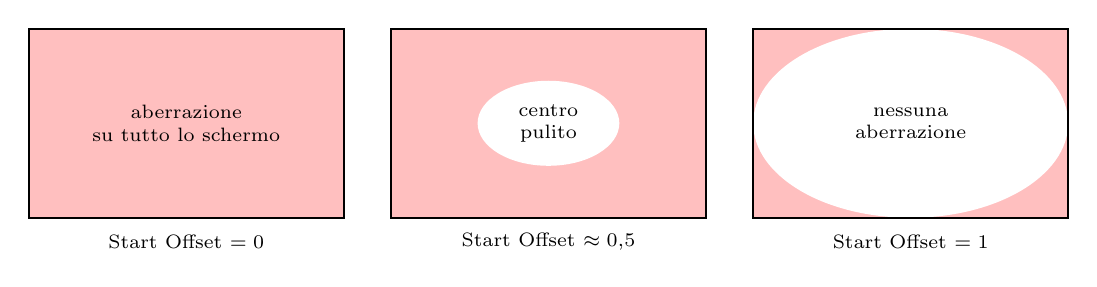
\begin{tikzpicture}[font=\scriptsize, x=1cm, y=1cm]
  \foreach \xs/\r/\lab in {0/0.0/{Start Offset $=0$}, 4.6/0.9/{Start Offset $\approx 0{,}5$}, 9.2/2.0/{Start Offset $=1$}} {
    \begin{scope}[xshift=\xs cm]
      \begin{scope}
        \clip (0,0) rectangle (4,2.4);
        \fill[red!25] (0,0) rectangle (4,2.4);
        \fill[white] (2,1.2) ellipse ({\r} and {\r*0.6});
      \end{scope}
      \draw[thick] (0,0) rectangle (4,2.4);
      \node at (2,-0.3) {\lab};
    \end{scope}
  }
  \node[align=center] at (2,1.2) {aberrazione\\su tutto lo schermo};
  \node[align=center] at (6.6,1.2) {centro\\pulito};
  \node[align=center] at (11.2,1.2) {nessuna\\aberrazione};
\end{tikzpicture}
\caption{Lo Start Offset della Chromatic Aberration: dal centro dello schermo fino al valore
impostato l'immagine resta pulita, oltre compare la separazione dei canali. A 1 l'effetto
sparisce. Ricostruzione schematica.}
\label{ue16:fig:chromatic}
\end{figure}

\paragraph{Approfondimento: aberrazione e accessibilità.} L'aberrazione cromatica imita un
difetto degli obiettivi reali, che non fanno convergere nello stesso punto le diverse
lunghezze d'onda: per questo è più forte ai bordi. Il consiglio del docente coincide con una
pratica diffusa dell'accessibilità: effetti come aberrazione, motion blur, vignettatura forte e
\emph{film grain} affaticano la vista o danno nausea a una parte dei giocatori, e molti giochi
offrono un'opzione per disattivarli. In Unreal si può farlo modificando a runtime le proprietà
del post process (per esempio il \emph{Post Process Settings} di una camera o di un volume da
Blueprint) oppure, per un picco di breve durata come la flashbang, animando l'intensità con una
\emph{Timeline}, lo strumento visto nelle prime lezioni del corso (funzionamento generale
dell'engine). Totten, nel capitolo 5, ricorda che l'horror lavora sull'incertezza percettiva
(l'ombra, la nebbia): l'aberrazione dell'esempio lovecraftiano è la versione
``sullo schermo'' della stessa strategia.

% ---------------------------------------------------------------------
\section{Il Lens Flare}
\label{ue16:sec:flare}

\paragraph{Che cos'è.} ``Questa è un'altra molto comune, molto vista'': ``forse è il tipo di
post-process con cui siamo più familiari'', perché si vede spesso anche nelle immagini delle
fotocamere. È la ``scomposizione dello spettro della luce'': dentro il volume la luce viene
scomposta, e si vedono ``gli esagoni che si creano''. Si può usare ``per diecimila motivi'':
per esempio quando il personaggio è appena uscito all'aperto dopo essere stato al chiuso, e la
scomposizione ``ci accoglie e ci dà un'idea di quanto effettivamente il sole sia forte'', o una
luce in generale.

\paragraph{I parametri.}
\begin{itemize}
  \item \textbf{Intensity}: quanto è forte. ``Se non ricordo male'' è influenzato anche dal
        \textbf{bloom}: ed ``esatto'', aumentando l'intensità del bloom il lens flare diventa
        più sfumato.
  \item \textbf{Tint}: il colore del flare, ``magari prendiamo questo flare violaceo''; si
        può anche modificare a mano il riferimento dei canali RGB.
  \item \textbf{Bokeh Size} (``poke size'': ``sono ignorante su come si pronuncia''): la
        grandezza di ``non lo so neanche come chiamarli, dei cristalli, degli esagoni della
        scomposizione della luce'', per un effetto più o meno scomposto (il docente toglie il
        blu per farlo vedere meglio).
  \item \textbf{Threshold}: ``funziona sempre nello stesso modo'', la soglia minima di
        luminosità per avere l'effetto.
  \item \textbf{Bokeh Shape}: ``devo essere onesto, non ho mai trovato un'utilità a questa
        cosa'', ma si può cambiare la forma dei cristalli con una \textbf{texture}. Quella di
        default si chiama, nella trascrizione, ``Presize default all''; cambiandola si hanno
        cerchi, pentagoni, ``qualsiasi texture abbiamo'': l'icona di un bersaglio, ``un'immaginina
        con delle stelline''. Le texture troppo dettagliate non rendono (``non si nota
        effettivamente il dettaglio''), ma per una questione di forma funzionano; la texture
        porta con sé anche il colore.
  \item \textbf{Tints}: per personalizzare ``al 100\%'' il flare, si può modificare ``ogni
        singolo cristallino'': ce n'è uno viola, uno blu, uno verde, e si decide quali colori
        dello spettro ``risultano maggiormente''. Sono numerati da 0 a 7 (la trascrizione elenca
        ``0, 1, 2, 3, 4, 5, 7'').
\end{itemize}
``Il lens flare lo teniamo, che insomma è piacevole averlo.''

\paragraph{Approfondimento: un difetto che diventa linguaggio.} Il lens flare è un riflesso
interno fra le lenti di un obiettivo, e i suoi esagoni hanno la forma del diaframma; in
Unreal Engine~5 il lens flare del post process è un effetto \emph{image-based}, calcolato a
partire dalle zone più brillanti dell'immagine (per questo dipende dal bloom e dalla soglia),
e la \emph{Bokeh Shape} è appunto la sagoma del diaframma simulato. Nel cinema e nei giochi il
flare comunica ``guardi verso una luce forte'' e, spesso, ``stai guardando attraverso una
camera'': usato ovunque, indebolisce l'idea di una visione in prima persona; usato al momento
giusto, come l'uscita all'aperto del docente, è un segnale di passaggio. Funzionamento generale
dell'engine.

% ---------------------------------------------------------------------
\section{La Depth of Field}
\label{ue16:sec:dof}

\paragraph{Mettere a fuoco.} ``Un'altra cosa molto importante che possiamo utilizzare nel
momento in cui andiamo a fare un render di un'immagine, ma anche quando dobbiamo gestire le
distanze'', è la \textbf{Depth of Field} (la profondità di campo). Permette ``una serie di
modifiche di messa a fuoco'': si modifica la \textbf{distanza focale}, cioè a quale distanza si
mette a fuoco. Nella prova c'è ``una leggera sfocatura'', e più in là ``qualcosa di meno messo a
fuoco, ma comunque non visibilissimo'': ``mettiamo che il nostro personaggio sia vagamente
miope, insomma, vedrà in questo modo qui''.

\paragraph{Gli altri parametri.} Il docente ricorda altri parametri che permettono di
determinare ``la distanza a cui vediamo il blur e l'intensità del blur'': ``quale sia la forza
della sfocatura e da quale distanza venga effettivamente attivata''. Ma ``ricordo funzionasse
in maniera diversa'': ``credo che sulla 4 funzioni in maniera diversa''. Promette di
controllare durante la pausa e di riferire le eventuali modifiche; dopo la pausa, però, la
trascrizione non riporta più nulla sulla depth of field.

\paragraph{Approfondimento: la profondità di campo in Unreal Engine~5.} La differenza che il
docente ricorda c'è davvero. In Unreal Engine~4 esistevano più metodi (\emph{Gaussian},
\emph{Bokeh}, \emph{Circle}), ciascuno con parametri propri come le regioni di transizione
vicina e lontana; in Unreal Engine~5 su PC e console resta di fatto un solo metodo, il
\emph{Cinematic} DOF, i cui parametri principali sono la \emph{Focal Distance} (la distanza
di messa a fuoco, in centimetri), l'\emph{Aperture} o \emph{f-stop} della camera (più è basso,
più la profondità di campo è stretta) e la dimensione del sensore; sono presenti anche
\emph{Depth Blur km for 50\%} e \emph{Depth Blur Radius}, che aggiungono una sfocatura di
distanza indipendente dalla messa a fuoco. Il \emph{Mobile Depth of Field} che il docente vede
nella lista della Camera Actor è la versione semplificata per dispositivi mobili, con distanze
di transizione esplicite, ed è probabilmente il modello di funzionamento che ricordava. Sulla
Camera Actor (\emph{Cine Camera Actor}) la messa a fuoco si regola dalle \emph{Focus Settings},
anche in modo automatico seguendo un actor (funzionamento generale dell'engine). In un gioco
la profondità di campo è utile soprattutto per i menu, i dialoghi e le schermate, dove guida lo
sguardo verso il soggetto: è la stessa funzione che Totten, nel capitolo 7, attribuisce alla
cinematografia, ``attirare l'attenzione del giocatore'' sugli elementi che il designer vuole
fargli vedere.

% ---------------------------------------------------------------------
\section{Il Color Grading}
\label{ue16:sec:grading}

\paragraph{La cosa più famosa.} ``Forse la cosa più famosa per cui è conosciuta e utilizzata
la post-produzione'' è la \textbf{color correction}: applicare all'immagine ``un nuovo stile, un
nuovo tipo di colore'' con una serie di parametri. Il docente richiude tutte le sezioni per
vederle una per una.

\paragraph{Temperature.} ``Di base, il color grading parte dalla \textbf{temperatura}'': una
scena più calda o più fredda, da un estremo all'altro, con ``questa renderizzazione più
giallastra'' o ``completamente sbiancata e bluastra''. Poi la \textbf{tinta} (\emph{Tint}), per
spingere la scena verso il magenta o verso il verde.

\paragraph{Global, Shadows, Midtones, Highlights.} Oltre alla temperatura ci sono i parametri
``che ci permettono di fare una customizzazione più completa'': \textbf{Global},
\textbf{Shadows}, \textbf{Midtones} (``mittons'') e \textbf{Highlights}. Sono la possibilità
di fare color correction su tutta la scena (Global), solo sugli scuri, ``nelle parti più buie,
nelle ombre'' (Shadows), ``nei grigi, nei medi'' (Midtones) e ``nelle luci, nelle parti più
illuminate'' (Highlights) (figura~\ref{ue16:fig:grading}).

\paragraph{Cinque sottoparametri.} ``Funzionano tutti allo stesso modo'': ognuno ha la stessa
lista di \textbf{Saturation}, \textbf{Contrast}, \textbf{Gamma}, \textbf{Gain} e
\textbf{Offset}, da attivare con la spunta ed espandere con la freccia. Con la saturazione si
decide quanto la scena sia satura o desaturata, con lo slider sotto. (A questo punto la
trascrizione si perde per diverse righe in un blocco ripetuto senza senso; quando riprende, il
docente sta parlando del \textbf{contrasto}.) Con il contrasto si gioca sulla differenza ``fra
le luci e le ombre'': la si può accentuare o appiattire, ``una sorta di maschera di contrasto
del colore''. ``Stessa cosa gamma e gain'': moltiplicano la color correction della scena, e si
alzano o abbassano per modificare il colore.

\begin{figure}[htbp]
\centering
\begin{tikzpicture}[font=\scriptsize, x=1cm, y=1cm]
  \shade[left color=black, right color=white] (0,0) rectangle (12,0.7);
  \draw[thick] (0,0) rectangle (12,0.7);
  \draw[thick] (0,1.0) -- (4,1.0);
  \node at (2,1.3) {\textbf{Shadows}: ombre};
  \node at (6,1.3) {\textbf{Midtones}: grigi, medi};
  \node at (10,1.3) {\textbf{Highlights}: luci};
  \draw[thick] (4,0) -- (4,1.1); \draw[thick] (8,0) -- (8,1.1);
  \draw[thick, {Stealth[length=1.6mm]}-{Stealth[length=1.6mm]}] (0,1.8) -- (12,1.8) node[midway, above] {\textbf{Global}: tutta la scena};
  \node[align=center, draw, rounded corners=2pt, fill=gray!10, inner sep=4pt] at (6,-0.9)
    {in ognuna: Saturation $\cdot$ Contrast $\cdot$ Gamma $\cdot$ Gain $\cdot$ Offset};
  \node[align=center, draw, rounded corners=2pt, fill=orange!10, inner sep=4pt] at (6,-1.8)
    {prima, per tutta l'immagine: Temperature (caldo / freddo) e Tint (magenta / verde)};
\end{tikzpicture}
\caption{Le zone del Color Grading. Global agisce su tutta l'immagine, Shadows, Midtones e
Highlights sulle zone scure, medie e chiare; ciascuna ha gli stessi cinque sottoparametri.
I confini fra le zone sono sfumati e regolabili. Ricostruzione schematica.}
\label{ue16:fig:grading}
\end{figure}

\paragraph{Uno strumento avanzato.} ``Il post-process è un elemento molto molto avanzato'':
non perché sia difficile da usare, ``ma nel senso che è difficile ottenere esattamente il
risultato che volete''. È un oggetto con cui ``dovete sperimentare, mettervi là, fare
esperienza'' di come funziona e di quali possibilità ha. ``Se dovessimo esplorarlo al 100\%
ci vorrebbe molto di più di una lezione, e probabilmente non sarei neanche la persona adatta.''
Il docente ha mostrato le lenti ``che potreste utilizzare di più'' per creare un certo
\emph{mood} e un certo tipo di scena; si ferma qui per parlare di altre cose ``ugualmente
importanti'', ``più basilari forse, meno avanzate''. Chi vuole può partire da questa base:
mettere in scena il proprio post process e ``smontarlo un pochino''.

\paragraph{Prima le luci, poi il post process.} La post produzione ``influisce grandemente
sulla luce'': a seconda del tipo di luce in scena si avranno effetti diversi. L'ordine giusto:
prima si costruisce l'illuminazione, ``come abbiamo visto con i light actor qualche lezione
fa'', e solo quando le luci sono posizionate si fa questo lavoro. ``Capisco che è stato molto
brutale e molto rapido'', ma ``più che mostrarvi gli elementi di base e incitarvi a provare a
sperimentare'' non c'è tempo. ``Oggi purtroppo corriamo un po'.''

\paragraph{Approfondimento: colore e significato.} Il color grading di Unreal segue il
modello dei programmi di correzione colore del cinema: Saturation, Contrast, Gamma, Gain e
Offset sono i classici controlli di \emph{lift-gamma-gain} applicati per zone, e i confini
fra Shadows, Midtones e Highlights si regolano con \emph{Shadows Max} e \emph{Highlights Min};
per un controllo totale si può usare una \emph{Color Grading LUT}, una tabella di colori
preparata in un programma esterno (funzionamento generale dell'engine). Totten, nel capitolo 4
(``Basic Color Theory''), fornisce il vocabolario per scegliere: i colori \emph{analoghi}
(tre colori vicini sulla ruota, come blu, blu-viola e viola) creano un'atmosfera armonica e,
in quel caso, ``un senso cupo o freddo''; rosso, rosso-arancio e arancio danno una sensazione
calda; i \emph{complementari} (opposti sulla ruota) creano contrasto. È esattamente il
``posto lugubre'' del docente, caricato di verdi, blu e viola. L'esempio di Totten è
\emph{Bioshock Infinite}: una cappella dominata dal blu in cui le uscite sulla strada
principale sono segnate da elementi complementari, una luce arancione o un fedele in tunica
bianca, mentre i passaggi secondari restano in tinte analoghe. Il color grading regola il
colore dominante; il contrasto che guida il giocatore va poi costruito con le luci e gli
oggetti.

% ---------------------------------------------------------------------
\section{La domanda sull'effetto in due toni}
\label{ue16:sec:duetoni}

\paragraph{La domanda.} Prima di passare al packaging arriva una domanda in chat: ``si possono
applicare effetti di luce più estremi, magari su altri programmi?'' Per esempio ``rendere il
livello in due toni'', ``solo rosso e nero'', per ottenere ``un effetto tipo
\textbf{Limbo}''. ``Sì, si può fare, ma anche già soltanto all'interno di Unreal, utilizzando
un post process volume.''

\paragraph{La zanzara e il cannone.} Il docente sposta però la questione: non è tanto ``se
Unreal lo può fare oppure no'', ma ``per fare quella cosa, è davvero necessario utilizzare
Unreal?'' Se l'idea è creare qualcosa di esteticamente molto semplice, in bianco e nero, si
può forse realizzarlo con altri engine. ``Teniamo sempre a mente che Unreal è un engine pesante
che fa le cose in maniera pesante.'' Se si vuole rifare Limbo, ``che magari è anche in 2D'' e
quindi più semplice, e lo si fa in Unreal, ``stiamo sparando a una zanzara con un cannone'':
``la zanzara l'ammazziamo, però smontiamo pure quello che c'è dietro''. Quanto agli ``altri
programmi'': se si fa un'immagine in Unreal, uno screenshot di un ambiente, e la si modifica
``in post'' con un programma di fotoritocco, ``sì, lo posso fare''.

\paragraph{Mallory.} Lo studente cita un gioco, ``Mallory'' (``Mellori'' più avanti; il nome
esatto non è ricostruibile dalla trascrizione), un titolo per Switch fatto in Unreal, e
condivide dei link. Il docente non lo conosce: ``poi me lo guardo durante la pausa''. In ogni
caso, ``se è fatto in Unreal si può fare tranquillamente'': l'idea stessa del Post Process
Volume è avere un oggetto in scena che permette di passare da un tipo di post produzione a un
altro o di controllarla meglio; ``una volta che mi impratichisco con lo strumento posso fare
un po' quello che mi pare''. Serve però anche gestire bene l'illuminazione: ci si costruisce
l'illuminazione ``come è gestita in quel titolo'' e poi la si modifica a posteriori. (Il
seguito, dopo la pausa, è nella sezione~\ref{ue16:sec:pausa}.)

\paragraph{Approfondimento: scegliere l'engine.} La metafora del cannone tocca un tema di
produzione: il costo di un engine non è solo la licenza, ma il peso dei progetti, i tempi di
compilazione degli shader e del packaging (che il docente sperimenterà di lì a poco) e le
macchine richieste ai giocatori, come ha scoperto lo studente con il portatile che ``non
reggeva''. Per un gioco 2D stilizzato un engine più leggero è spesso la scelta più efficiente;
Unreal ha comunque strumenti 2D (\emph{Paper2D}, gli sprite e i flipbook citati nella lezione
precedente). Un effetto ``in due toni'' in Unreal si ottiene con un \emph{Post Process
Material}: un materiale con dominio \emph{Post Process}, assegnato nei \emph{Rendering
Features} del volume (\emph{Post Process Materials}), che legge il colore della scena e lo
riduce a due colori secondo una soglia di luminosità (funzionamento generale dell'engine).
Totten, nel capitolo 4, usa proprio \emph{Limbo} come esempio di linguaggio visivo: il gioco
gioca il suo stile a silhouette contro le convenzioni del giocatore, come nel puzzle della
pressa in cui il ``pulsante'' rialzato non è il vero meccanismo. Lo stile in due toni, lì, non
è un filtro sopra il gioco: è parte delle regole con cui il giocatore legge lo spazio.

% ---------------------------------------------------------------------
\section{Il packaging: che cos'è e dove si avvia}
\label{ue16:sec:packaging}

\paragraph{Che cos'è.} ``Il packaging è un processo che viene fatto principalmente da Unreal
Engine, in realtà, per cui noi dobbiamo andare a curare soltanto alcune impostazioni.'' È ciò
che ``ci consente di andare a creare un \textbf{eseguibile} con quello che noi abbiamo
all'interno dell'editor''.

\paragraph{Platforms.} Il packaging si avvia dal pulsante \textbf{Platforms} della barra degli
strumenti. Scendendo si vedono ``tutte le varie piattaforme per cui potremmo sviluppare
qualcosa'': \textbf{Android}, \textbf{iOS}, \textbf{Linux}, \textbf{Mac}, \textbf{Windows}.
Accanto ad alcune c'è ``sempre questo segnale di attenzione'': il docente è su Windows, e il
progetto ``non è gestito o pensato'' per funzionare anche sugli altri sistemi. Nella voce
\textbf{Windows} ci sono il \textbf{Package Project}, ``il pulsantone che io premo se voglio far
partire questo processo'', e la scelta della \textbf{configurazione}. ``Queste sono pochissime
impostazioni, e non sono neanche lontanamente tutte quelle che ci servono'': le altre sono nei
\textbf{Project Settings}, la ``macro sezione di setting e di impostazioni per tutto il nostro
progetto'' già vista con Igor (figura~\ref{ue16:fig:packaging}).

\paragraph{Il plugin di Fab.} Un'altra finestra che può servire è quella dei \textbf{Plugins},
che permette di attivare e disattivare i plugin. ``Da quello che so, il plugin di
\textbf{Fab} dà dei problemi con il packaging'': quindi, prima di impacchettare, lo si
disattiva. ``Non so se è stato risolto. Potrebbe essere stato risolto, dovrei informarmi.''

% ---------------------------------------------------------------------
\section{Le impostazioni del progetto}
\label{ue16:sec:impostazioni}

\paragraph{Maps \& Modes.} Nei Project Settings, nella pagina \textbf{Maps \& Modes}, ``oltre
alla Game Mode'', ci sono le \textbf{Default Maps}: \textbf{Editor Startup Map} e
\textbf{Game Default Map}.
\begin{itemize}
  \item L'\textbf{Editor Startup Map} è la mappa con cui si apre l'editor: se la si cambia,
        ``ogni volta che io aprirò questo progetto lui mi partirà da quell'altra mappa'', e per
        tornare al livello di prima bisognerà riaprire a mano la Third Person Map.
  \item La \textbf{Game Default Map} è ``allo stesso modo la mappa di partenza che avremo
        all'interno del nostro eseguibile''. Se il gioco ha un menu che porta alla mappa di
        gioco, non si mette la Third Person Map: ``di solito quello che si fa è mettere un
        \textbf{menu principale}'', o una schermata che, dopo aver cliccato qualche pulsante,
        porta alle mappe che si vogliono giocare.
\end{itemize}
Sono due impostazioni importanti: ``se mai vi capiterà di dire: oddio, dove è andata la mia
mappa, perché si è aperto così, dove sono finito, cosa è successo''; oppure ``per quale motivo
ho fatto il packaging e non mi fa partire da dove dico io'': è la Game Default Map da
modificare. (Il docente scorre altre voci della pagina, ``ma questa non è necessaria'', senza
nominarle.)

\paragraph{Supported Platforms.} Un'altra pagina è quella delle \textbf{Supported Platforms}.
Di default è impostata su \textbf{All Platforms}; togliendo la spunta e lasciando solo ciò che
interessa si può avere, per esempio, soltanto \textbf{Windows} come piattaforma per il
packaging, ``perché il nostro progetto magari non supporta tutti gli altri sistemi
operativi''.

\paragraph{La pagina Packaging.} ``Ultima cosa, ma la più importante'': c'è una pagina tutta
dedicata al \textbf{packaging}. ``Sono un sacco di informazioni, un sacco di parametri'', ma
``la cosa positiva è che la maggior parte di questi parametri sta bene come sta'': non servono
``modifiche assurde''. Alcune voci si vedono subito, altre solo aprendo gli
\textbf{Advanced}. Le prime: \textbf{Build}, ``va bene così'' (l'opzione ``if project has code
or running a locally built editor'', che lascia decidere all'engine se compilare); poi la
\textbf{Build Configuration}.

% ---------------------------------------------------------------------
\section{Le configurazioni di build}
\label{ue16:sec:build}

\paragraph{Cinque configurazioni, tre disponibili.} La \textbf{Build Configuration} decide
``che tipo di configurazione avrà il nostro eseguibile'': \textbf{Debug}, \textbf{DebugGame},
\textbf{Development}, \textbf{Test} e \textbf{Shipping}. ``Per la build che abbiamo scelto''
ne sono attive soltanto tre (le stesse che si ritrovano poi nel menu Platforms: DebugGame,
Development e Shipping). Le differenze (tabella~\ref{ue16:tab:build}):
\begin{itemize}
  \item \textbf{Debug} e \textbf{DebugGame} ``sono modalità di debug'': un eseguibile in cui
        c'è ancora una \textbf{console di comandi} per inserire comandi, fare aggiustamenti,
        ``vedere le linee, vedere quello che sta succedendo, vedere dei text che vengono
        printati''. ``È una versione super di test.''
  \item \textbf{Development} è ``la configurazione di default di Unreal''. Rimuove la maggior
        parte della struttura di debug, aumenta un po' l'ottimizzazione della build, ``ma
        mantiene comunque alcuni strumenti che possono essere utilizzati per il testing''. ``Se
        debug è un eseguibile che può essere di uso a un \textbf{programmatore}, development può
        essere di uso a un \textbf{designer}'': si può ancora modificare qualcosa e usare degli
        input, ma serve soprattutto per testare e poi ritoccare in engine.
  \item \textbf{Shipping} è la modalità ``per la distribuzione'': ``il progetto finito, il
        gioco che le masse giocheranno, si spera le masse''. È ``la versione più ottimizzata
        possibile della build'', ``la build da vendita, praticamente''.
\end{itemize}

\paragraph{Shipping non ottimizza da solo.} ``Aspettate: questo non vuol dire che lui vi
ottimizzi le cose in automatico.'' L'ottimizzazione ``è tutto un discorso a parte, che va fatto
separatamente'': far sì che non ci siano troppe linee di codice, che non ci siano texture a
qualità troppo alta o non utilizzate, eccetera. Shipping ``vuol dire semplicemente che lui va a
togliere tutta una serie di strumenti che non servono più''.

\begin{table}[htbp]
\centering
\small
\begin{tabular}{@{}p{2.3cm}p{5.6cm}p{3.0cm}p{3.1cm}@{}}
\toprule
\textbf{Configurazione} & \textbf{Che cosa contiene (lezione)} & \textbf{Per chi} &
\textbf{Nota} \\
\midrule
Debug & console di comandi, linee, testi stampati: ``versione super di test'' &
programmatore & richiede un progetto con codice C++ \\
DebugGame & come sopra, debug del codice di gioco & programmatore & disponibile \\
Development & default di Unreal; meno debug, un po' più ottimizzata, alcuni strumenti di test
& designer, tester & disponibile; console attiva \\
Test & vicina a Shipping, con qualche strumento di profilazione & QA & richiede codice C++ \\
Shipping & la versione finale, senza strumenti di sviluppo & i giocatori & disponibile; non
ottimizza da sola \\
\bottomrule
\end{tabular}
\caption{Le cinque configurazioni di build. Nel progetto del docente ne sono attive tre; la
colonna ``Nota'' integra con il funzionamento generale dell'engine.}
\label{ue16:tab:build}
\end{table}

\paragraph{Le lingue.} Aprendo gli Advanced si trovano le \textbf{lingue} del packaging
(\emph{Localizations to Package}): ``possiamo andare a selezionare che tipo di lingue dovranno
essere utilizzate''. ``Di default c'è solo l'inglese.'' Se si è localizzato qualcosa, per
esempio perché ci sono già impostazioni e parametri che fanno riferimento a certe lingue, qui
si scelgono quelle da includere.

\paragraph{Approfondimento: le configurazioni secondo Romero e Sewell.} Romero e Sewell, nel
capitolo 12 (``Building and Publishing''), descrivono lo stesso percorso: \emph{Platforms}
$\rightarrow$ piattaforma $\rightarrow$ \emph{Package Project}, la scelta della cartella, la
finestra che avvisa che l'engine sta impacchettando e, in caso di problemi, ``i dettagli
dell'errore nella finestra dell'output log''. Prima, nei \emph{Project Settings}: la pagina
\emph{Description} (nome, miniatura, descrizione del progetto), la pagina \emph{Maps \& Modes}
(``spesso dovrete designare una mappa dedicata al menu principale come prima mappa da
caricare'', e assicurarsi che sia lei a gestire quale mappa si carica dopo) e la pagina della
piattaforma, dove per Windows si cambiano lo \emph{splash screen} e l'\emph{icona}
dell'eseguibile. Sulle configurazioni il libro precisa che nei progetti \emph{solo
Blueprint} le opzioni principali sono \textbf{Development}, che contiene informazioni di debug
utili a trovare errori, e \textbf{Shipping}, ``più pulita'', da usare per la versione da
distribuire; Debug e Test richiedono un progetto con codice C++ (ed è per questo che nel
progetto del docente sono spente). Il libro nomina anche la \emph{Staging Directory}, la
cartella in cui viene salvata la build, l'opzione \emph{For Distribution}, richiesta per
pubblicare su App Store o Google Play, e lo \emph{Zip Project} del menu File, che comprime i
file essenziali del progetto per passarlo a un'altra persona. Una nota importante dello stesso
capitolo: Unreal Engine~5 può creare build Windows solo da Windows e build macOS solo da macOS;
è il ``segnale di attenzione'' che il docente vede accanto alle altre piattaforme.

% ---------------------------------------------------------------------
\section{Le mappe e le cartelle da cucinare}
\label{ue16:sec:cook}

\paragraph{Cook only maps.} ``Fare il packaging di base vuol dire che lui prende tutto il
progetto e lo rende pronto per essere un eseguibile'', con un certo metodo di compressione.
Spuntando \textbf{Cook only maps} (``hook only maps'' nella trascrizione), invece, il
packaging usa ``unicamente le mappe'': si può dirgli di usare soltanto la Third Person Map, e
lui ``si vede cosa c'è dentro'', mette nel pacchetto ``tutto quello che serve per far funzionare''
quella mappa ``e non mette il resto delle cose''.

\paragraph{List of maps to include.} Insieme a Cook only maps serve la voce \textbf{List of maps
to include in a packaged build}. Si aggiunge un elemento, si clicca sui tre puntini e si cerca
la mappa: ``volete level 1, level 2, menu? Magari vi serve il menu''. Nel caso della prova
serve soltanto la Third Person Map (il file \texttt{.umap}): ``non serve andare a inserire anche
il build data'' (il file \texttt{\_BuiltData}) ``o lo \texttt{.uasset}''. Si possono aggiungere
altre mappe, copiarle, eliminarle.

\paragraph{Directories to never cook.} ``Un'altra cosa che ci torna utile'' è
\textbf{Directories to never cook}: le cartelle che non devono mai finire nel pacchetto. Si
aggiunge un elemento (``un index zero'') e si sceglie la cartella. Gli esempi:
\begin{itemize}
  \item ``nulla di \emph{GameApps}'' (il nome della cartella, nella trascrizione, è ``game
        apps'') ``deve finire dentro il packaging'';
  \item una cartella con ``tutta una serie di modelli 3D molto fighi'' che non si è riusciti a
        inserire e che magari si vogliono usare in un \textbf{DLC} più avanti.
\end{itemize}
I motivi sono due. Il primo è il \textbf{data mining}, ``diventato super popolare adesso'': i
file messi nel gioco ``possono essere ritrovati da chi va a scavare''. Il secondo: sono comunque
cose ``che vanno ad essere cucinate e vengono comunque inserite all'interno della build''.
Togliere le cartelle che non servono ``ci fa risparmiare giga'': un progetto più piccolo e più
semplice da gestire (tabella~\ref{ue16:tab:packaging}).

\begin{table}[htbp]
\centering
\small
\begin{tabular}{@{}p{4.6cm}p{2.8cm}p{6.6cm}@{}}
\toprule
\textbf{Impostazione} & \textbf{Dove} & \textbf{A che cosa serve} \\
\midrule
Package Project, configurazione & Platforms $\rightarrow$ Windows & avviare il packaging;
scegliere DebugGame, Development, Shipping o le impostazioni del progetto \\
Plugin di Fab & Edit $\rightarrow$ Plugins & disattivarlo prima del packaging (problemi
noti, forse risolti) \\
Editor Startup Map & Maps \& Modes & la mappa con cui si apre l'editor \\
Game Default Map & Maps \& Modes & la prima mappa dell'eseguibile: di solito il menu \\
Supported Platforms & Project Settings & limitare le piattaforme (per esempio solo Windows) \\
Build & Packaging & lasciare il default \\
Build Configuration & Packaging & Debug, DebugGame, Development, Test, Shipping \\
Localizations to Package & Packaging (Advanced) & le lingue incluse; default inglese \\
Cook only maps & Packaging (Advanced) & impacchettare solo ciò che serve alle mappe elencate \\
List of maps to include & Packaging (Advanced) & le mappe (\texttt{.umap}) da includere \\
Directories to never cook & Packaging (Advanced) & cartelle escluse: asset scartati, DLC,
spazio \\
Show Output Log & finestra del packaging & seguire il processo e trovare gli errori in rosso \\
\bottomrule
\end{tabular}
\caption{Le impostazioni del packaging viste a lezione, nell'ordine in cui il docente le
mostra.}
\label{ue16:tab:packaging}
\end{table}

\paragraph{Approfondimento: che cosa vuol dire ``cucinare''.} Il \emph{cooking} è la fase in
cui l'engine converte gli asset dal formato dell'editor a quello ottimizzato per la
piattaforma di destinazione: compila gli shader, comprime le texture, elimina i dati che
servono solo all'editor. Il packaging vero e proprio raccoglie poi gli asset cucinati in
archivi (\emph{.pak}, o \emph{IoStore} in Unreal Engine~5) accanto all'eseguibile. Con Cook
only maps disattivato l'engine cucina di norma tutto il contenuto del progetto, compresi gli
asset mai usati; con l'opzione attiva segue le \emph{reference} a partire dalle mappe
elencate. Un'avvertenza: un asset caricato solo per nome, a runtime (per esempio con un
percorso scritto in una stringa), non è una reference visibile al cook e rischia di restare
fuori; per questi casi esistono le voci \emph{Additional Asset Directories to Cook}. Anche
\emph{Directories to never cook} va usata con attenzione: se un asset escluso è referenziato
da una mappa inclusa, il cook segnala un errore o il gioco lo perde (funzionamento generale
dell'engine). Totten, nel capitolo 2, parla di \emph{modular design} e di ``schedule'' dei
pezzi di un livello: sapere fin dalla pre-produzione quali pezzi servono rende più facile
anche sapere, alla fine, che cosa lasciare fuori.

% ---------------------------------------------------------------------
\section{L'avvio del packaging e l'Output Log}
\label{ue16:sec:avvio}

\paragraph{Dove salvare.} Per avviare si torna al menu Platforms: lì si vedono le
configurazioni (``debug'', \textbf{Development} e \textbf{Shipping}, ``perché sono le tre
possibili''), oppure \emph{Use Project Setting}, cioè quelle della pagina Packaging. Il docente
sceglie \textbf{Development}. Con \textbf{Package Project} si apre una finestra che chiede dove
creare il pacchetto; il docente sceglie il desktop, e parte il processo, accompagnato da un
``suonino''.

\paragraph{La prima volta è lenta.} ``Fare un packaging la prima volta è molto lento'', anche
se è solo di una mappa. ``Dopo il primo packaging diventa tutto molto più veloce.'' Mentre
lavora (``parte \emph{Cancel}, chiaramente'', per interromperlo) si può aprire lo
\textbf{Show Output Log}: lì si vede tutto quello che sta succedendo. Scorrendolo (``con la
rotella del mio mouse che è rotta è tremendo'') si controlla se va tutto bene, se ci sono
errori o ``piccoli problemi'', o cose che creano problemi al packaging. In quel momento
l'engine sta facendo ``la compilazione degli shader''.

\paragraph{La scritta rossa.} ``Arriverà un punto in cui magari c'è una scritta rossa.'' La
scritta rossa ``vuol dire che c'è un problema che gli impedisce di fare il packaging''. Si legge
che cosa dice, si risolve quel problema, e si riprova.

\paragraph{Che cosa esce.} Se il processo finisce, nella cartella scelta si crea una cartella
che, ``se non gli viene dato un nome'', si chiama \textbf{Windows No Editor} (in Unreal
Engine~5 è semplicemente \emph{Windows}; \emph{WindowsNoEditor} era il nome di Unreal
Engine~4). Dentro c'è l'\textbf{eseguibile}: avviandolo parte il progetto, che in questo caso
sarebbe soltanto la Third Person Map, ``perché è l'unica mappa che gli abbiamo detto di
cucinare''. Il personaggio spawna sul \textbf{Player Start} e può andare in giro: ``non c'è un
obiettivo, non c'è una fine, non c'è nulla''.

\paragraph{I confini della mappa.} ``Chiaramente, per un packaging, non dovrebbero esserci
posti in cui puoi buttarti di sotto nel nulla, come il bordo della mappa''; né posti ``in cui
io non voglio che i giocatori vadano''. Nessuna domanda sul packaging. Siccome ci vorrà ``un
po' troppo tempo'', il docente anticipa la pausa, ``in modo che forse durante la pausa lui
finisca di calcolare'' e si possa vedere che cosa genera. Dopo la pausa: ``un paio di altri
attori'' utili quando si fa un livello, il Blueprint delle \textbf{spline}, ``che potete
utilizzare per un sacco di elementi diversi'', e, ``se ci avanza un po' di tempo'', le
\textbf{decal}, ``un altro strumento di decoro, di arredo'' per aggiungere dettagli in giro per
la mappa. ``Facciamo un 15 minuti di stop. Ci rivediamo alle 5 e mezza.''

\begin{figure}[htbp]
\centering
\begin{tikzpicture}[font=\scriptsize, x=1cm, y=1cm,
  ue16step/.style={draw, thick, rounded corners=2pt, fill=white, align=center, text width=2.6cm, minimum height=1.1cm, inner sep=3pt},
  ue16arr/.style={-{Stealth[length=1.8mm]}, thick}]
  \node[ue16step, fill=gray!10] (a) at (0,0) {Plugins:\\disattivare Fab};
  \node[ue16step, fill=blue!8] (b) at (3.3,0) {Maps \& Modes:\\Game Default Map\\(il menu)};
  \node[ue16step, fill=blue!8] (c) at (6.6,0) {Packaging:\\configurazione,\\lingue, mappe,\\cartelle escluse};
  \node[ue16step, fill=orange!12] (d) at (9.9,0) {Platforms $\rightarrow$\\Windows $\rightarrow$\\Package Project};
  \node[ue16step, fill=red!8] (e) at (9.9,-2.2) {Output Log:\\shader, cook;\\scritte rosse?};
  \node[ue16step, fill=green!12] (f) at (6.6,-2.2) {cartella \emph{Windows}\\con l'eseguibile};
  \node[ue16step, fill=green!12] (g) at (3.3,-2.2) {ritestare il gioco\\impacchettato};
  \node[ue16step, fill=green!12] (h) at (0,-2.2) {caricare (itch.io,\\Drive) e link\\su Discord};
  \draw[ue16arr] (a) -- (b); \draw[ue16arr] (b) -- (c); \draw[ue16arr] (c) -- (d);
  \draw[ue16arr] (d) -- (e); \draw[ue16arr] (e) -- (f); \draw[ue16arr] (f) -- (g);
  \draw[ue16arr] (g) -- (h);
  \draw[ue16arr, red!70!black] (e.east) -- ++(0.6,0) |- node[pos=0.25, right, align=left] {errore:\\risolvere\\e ripartire} (d.east);
\end{tikzpicture}
\caption{Il percorso del packaging come emerge dalla lezione, fino al consiglio finale di
ritestare il gioco impacchettato e condividerlo. Ricostruzione schematica.}
\label{ue16:fig:packaging}
\end{figure}

% ---------------------------------------------------------------------
\section{La pausa e Mallory}
\label{ue16:sec:pausa}

\paragraph{Il packaging non finisce.} Durante la pausa la trascrizione contiene soltanto il
blocco ripetuto già visto, che non appartiene alla lezione. Alla ripresa: ``purtroppo noi ci
siamo, ma Unreal ancora no, ancora non ho finito col packaging''. Il docente lo interrompe,
``perché sennò mi impedisce di fare altre robe'': ``non pensavo ci volesse così tanto tempo''.
Il risultato del packaging, quindi, non viene mostrato.

\paragraph{Mallory, visto.} Il docente ha guardato il gioco segnalato prima. ``Sembra molto
carino'': non l'ha potuto giocare, ma dal video ``sembra un platform simpatico con un bell'ambiente''.
Non gli è sembrato che ci sia ``un eccessivo utilizzo del post-process''. Quello che fanno
``sicuramente'' è cambiare il modo in cui vengono renderizzate luci e ombre: ``ci sono delle parti
con le ombre che sono molto rossastre rispetto alla luce, che magari è una luce più neutra'',
``una piccola vignettatura'' e ``un effetto di sfocatura messa davanti alla camera''. Lo
studente ha in mente anche altri titoli; il docente osserva che il genere platform ``ora come ora
è messo in mano agli indipendenti'': ``non ci sono più grossi titoloni che fanno quel tipo di
roba''. È giusto cercare ``cose carine fatte da persone in giro'', su Twitch o fra i piccoli
titoli su Steam. ``Purtroppo non è proprio il mio genere'', a parte ``i vecchi classiconi PS1,
PS2''.

\paragraph{Come rifare quell'effetto.} Le indicazioni del docente:
\begin{itemize}
  \item una \textbf{Dirt Mask}, come effetto di camera: una texture sovrapposta alla lente. Fra
        le texture del progetto non ce n'è una adatta; una ``un po' più fitta'' dà già ``questa
        specie di effetto statico, tra virgolette, sulla camera'', da gestire poi con i colori
        corretti (quella provata rende la Dirt Mask rossa: ``se riesci a fartela di effetto
        statico perfetto, potrebbe non essere male'');
  \item negli \textbf{Image Effects}, una piccola \textbf{vignettatura} (\emph{Vignette
        Intensity}), che ``va a scurire lo schermo'' nelle parti esterne e dà ``già di base'' un
        mood un po' più scuro;
  \item il resto ``è tutta \textbf{color correction}'': modificare i colori delle ombre per
        avvicinarli a quelli delle luci, desaturare un po' la scena (``c'è fondamentalmente una
        scala di grigio e in più c'è il rosso, barra rosa'') e mettere ``un accento sul rosso''
        dove c'è il rosso.
\end{itemize}

\paragraph{Monument Valley.} Mallory ricorda al docente, per la struttura dei livelli ``molto
geometrici, molto quadratosi'', i \textbf{Monument Valley}: ``non sono dei platform, sono dei
puzzle game misto opera estetica''. Si basano sull'\textbf{illusione ottica}: il personaggio
``cammina su un corridoio e poi improvvisamente inizia a camminare sulla parete e poi passa
dietro la scena'', e bisogna ruotare il livello per capire dove sta andando. ``Faccio fatica a
descriverli, però cercali, sono molto carini.'' Poi si torna al programma: ``post process,
rapidamente e bruttamente, ma lo abbiamo visto''.

\paragraph{Approfondimento: accentare un colore.} L'``accento sul rosso'' in una scena
desaturata è un'applicazione diretta del contrasto di Totten (capitolo 4): un elemento di un
colore diverso dal dominante attira l'attenzione, e se il colore è sempre lo stesso diventa un
segnale che il giocatore impara a leggere. In Unreal non c'è un controllo per ``desaturare
tutto tranne il rosso'' nel color grading standard: lo si ottiene con un Post Process Material
o, più semplicemente, desaturando con il post process e dando agli oggetti rossi materiali con
un po' di \emph{emissive}, così che restino saturi anche dopo la correzione. La vignettatura si
regola con \emph{Vignette Intensity} negli \emph{Image Effects}; la Dirt Mask nella sezione
\emph{Lens}, con \emph{Dirt Mask Texture}, \emph{Intensity} e \emph{Tint}, ed è visibile solo
dove c'è bloom (funzionamento generale dell'engine). Totten, nel capitolo 4, nota anche come
le associazioni dei colori passino nei giochi: rosso e verde per la salute, blu per la magia.

% ---------------------------------------------------------------------
\section{Le spline: che cosa sono}
\label{ue16:sec:spline}

\paragraph{Una linea.} Il docente ha preparato due Blueprint ``al volo prima di cominciare la
lezione''. Prima, però, ``che cos'è una spline?'' È un \textbf{component} che si può aggiungere
ai Blueprint, ma ``in realtà è proprio un tipo di oggetto'' con una funzione ben specifica, che
si usa anche per modificare il funzionamento del \textbf{landscape} (le \emph{landscape
spline}). Il docente crea un Blueprint di prova con un \textbf{Spline Component}; il tooltip
dice che è ``una spline shape che può essere usata per altri scopi, tipo animare oggetti''.
``È una linea, fondamentalmente.''

\paragraph{Punti e tangenti.} Messa in scena, la spline ``non è nient'altro che una linea'' che
si può allungare, curvare e arricchire di punti (figura~\ref{ue16:fig:spline}):
\begin{itemize}
  \item all'inizio ha \textbf{due punti}, l'inizio e la fine;
  \item cliccando sul punto finale compaiono altri due punti, la \textbf{tangente}; spostandola,
        la spline si curva;
  \item per creare \textbf{nuovi punti} si fa come quando si copia un oggetto: sulla freccia
        del gizmo, \textbf{Alt} premuto, si trascina, ``e ho fatto una copia''; ogni punto
        nuovo curva la linea, si può alzare, spostare, fino a costruire ``una figura, una
        struttura'';
  \item con il tasto destro, \textbf{Delete Spline Point} elimina un punto (la spline si
        riempie da sola fra i punti rimasti, ``lui autofilla'') e \textbf{Add Spline Point
        Here} ne aggiunge uno.
\end{itemize}

\begin{figure}[htbp]
\centering
\begin{tikzpicture}[font=\scriptsize, x=1cm, y=1cm]
  \draw[very thick, blue!70!black] (0,0) .. controls (2,0) and (2.5,2) .. (4.5,2)
                                   .. controls (6.5,2) and (6.5,0) .. (8.5,0.3)
                                   .. controls (10,0.5) and (10.5,1.6) .. (11.5,1.8);
  \foreach \p/\n in {(0,0)/0, (4.5,2)/1, (8.5,0.3)/2, (11.5,1.8)/3} {
    \fill[white, draw=black, thick] \p circle (3pt);
    \node[below=4pt] at \p {punto \n};
  }
  % tangente sul punto 1
  \draw[thick, red!70!black, {Stealth[length=1.5mm]}-{Stealth[length=1.5mm]}] (2.9,2) -- (6.1,2);
  \fill[red!70!black] (2.9,2) circle (2pt); \fill[red!70!black] (6.1,2) circle (2pt);
  \node[above, red!70!black] at (4.5,2.1) {tangente: lunghezza e verso curvano la linea};
  \node[align=left, anchor=west] at (0,-1.1) {Alt + trascinamento su un punto: nuovo punto \quad
    tasto destro: Add Spline Point Here, Delete Spline Point};
  \node[align=left, anchor=west] at (0,-1.6) {segmenti = punti $-$ 1 (qui 4 punti, 3 segmenti: indici da 0 a 2)};
\end{tikzpicture}
\caption{Una spline con quattro punti. Ogni punto ha una posizione e una tangente; i segmenti
sono uno in meno dei punti. Ricostruzione schematica.}
\label{ue16:fig:spline}
\end{figure}

% ---------------------------------------------------------------------
\section{A che cosa servono le spline}
\label{ue16:sec:usi}

\paragraph{Il muro di spine.} ``Immaginate di poter piazzare un oggetto lungo questa linea, o
di poter modellare un oggetto lungo questa linea.'' La storia che il docente racconta gli è
successa ``quando stavo in Accademia'', quando aveva cominciato a ``smanettare con questo
strumentino''. Bisogna creare un \textbf{muro di spine}, come nella \emph{Bella addormentata
nel bosco}, ``tutte le spine attorno al castello''. Due strade:
\begin{itemize}
  \item andare dall'``amico grafico'' e chiedergli ``un muro di spine fatto così, così e così'':
        una mesh ``non particolarmente impegnativa'', ma che richiede tempo e che, se va
        modificata, deve tornare in un software di modellazione come \textbf{Blender} o
        \textbf{Maya};
  \item ``una roba un po' più intelligente'': farsi creare soltanto un \textbf{cilindro di
        spine} e \emph{replicarlo} lungo una spline, così che la mesh ``viene ricreata e viene
        modificata sulla base della spline'', seguendone l'andamento.
\end{itemize}

\paragraph{Altri usi.} ``Al di là di questa cosa'', la struttura serve per molte cose: una
\textbf{pista} per un gioco di macchine (``vi create un blueprint di spline con la strada''); un
\textbf{muro} più stondato nel blockout o nella gym, per esempio ``che sale a spirale verso
l'alto'', quando ``non avete nulla che ve lo fa fare in maniera comoda''. Il docente lo mostra
``in due forme, in due versioni'': una ``più semplice e più brutta'', l'altra ``un po' più
funzionale''. I Blueprint si chiamano \textbf{Spline by Length} e \textbf{Spline by Point}.

\paragraph{La mesh del tubo.} Per la prova usa un tubo, ``un oggetto molto semplice'' che è
anche nel progetto degli studenti: \textbf{SM\_PipeSplineBody} (``Sm pipe spline body''). Il
docente prima dice che ``non è fatto benissimo per essere un oggetto da spline'', poi si
corregge: ``ho detto una cazzata, l'avevo vista in maniera veloce prima''. Funziona bene
perché è \textbf{segmentato}: ha i suoi triangoli e ``questa spezzatura in orizzontale'', è
\textbf{modulare} (``cilindro, cilindro, cilindro''). Questo permette al Blueprint di
replicarlo ``senza andarlo a spezzare'', perché la struttura del tubo viene replicata cilindro
per cilindro. Nella prima versione, allungando la spline il cilindro si allunga; piegandola,
si piega ``però si spezza'', perché è fatta ``in una maniera meno ottimale''; nella seconda ``si
spacca'' ancora, ma ``dovrebbe notarsi di meno''. La differenza (figura~\ref{ue16:fig:pointlength}):
``il primo blueprint, by point, \emph{stretcha} l'oggetto; questo invece ricrea l'oggetto per
lunghezza, quindi è un pochino più fedele''.

\begin{figure}[htbp]
\centering
\begin{tikzpicture}[font=\scriptsize, x=1cm, y=1cm]
  % by point
  \node[anchor=west] at (0,2.9) {\textbf{Spline by Point}: una mesh per ogni segmento, stirata fino al punto successivo};
  \foreach \a/\b/\c in {0/4.2/blue!20, 4.2/6.2/green!20, 6.2/12/orange!20} {
    \draw[thick, fill=\c] (\a,1.6) rectangle (\b,2.4);
  }
  \foreach \x in {0,4.2,6.2,12} \fill[black] (\x,2.0) circle (2.2pt);
  \node at (2.1,2.0) {stirata}; \node at (5.2,2.0) {schiacciata}; \node at (9.1,2.0) {molto stirata};
  % by length
  \node[anchor=west] at (0,1.0) {\textbf{Spline by Length}: una mesh ogni \emph{Mesh Length}, sempre proporzionata};
  \foreach \i in {0,...,5} {
    \draw[thick, fill=blue!20] ({\i*2},-0.2) rectangle ({\i*2+2},0.6);
  }
  \foreach \x in {0,12} \fill[black] (\x,0.2) circle (2.2pt);
  \draw[{Stealth[length=1.4mm]}-{Stealth[length=1.4mm]}] (0,-0.45) -- (2,-0.45) node[midway, below] {Mesh Length (250)};
  \node[align=center] at (9,-0.7) {anche con due soli punti: tanti pezzi quanti\\ne stanno nella lunghezza della spline};
\end{tikzpicture}
\caption{Le due versioni del Blueprint su una spline dritta. Per punto, il numero di mesh è
uno in meno dei punti e ciascuna si deforma fino al punto successivo; per lunghezza, il numero
di mesh dipende dalla lunghezza della spline divisa per quella della mesh. Ricostruzione
schematica.}
\label{ue16:fig:pointlength}
\end{figure}

% ---------------------------------------------------------------------
\section{Il Blueprint per punto}
\label{ue16:sec:bypoint}

\paragraph{La struttura.} Nel \textbf{Spline by Point} la viewport contiene la spline e
``un oggetto che poi gli abbiamo attaccato con un nodo''; l'Event Graph è vuoto, e tutto è nel
\textbf{Construction Script}. ``È una struttura abbastanza semplice'', usabile ``tranquillamente''
per un lavoro di blockout, ``di prototipazione''. Alcune cose il docente le fa ``un po' più
veloce, perché probabilmente le avete già viste anche con Igor''. Il grafo
(figura~\ref{ue16:fig:grafopoint}):
\begin{enumerate}
  \item un \textbf{For Loop}, ``perché dobbiamo loopare un oggetto''. Il \emph{First Index} è
        \textbf{0}, ``la base dell'indice''. Il \emph{Last Index} viene dal numero di punti della
        spline, preso trascinando la spline nel grafo e usando \textbf{Get Number of Spline
        Points}; al numero si \textbf{sottrae 2}. Il motivo detto a lezione: ``sono i due punti
        che abbiamo già di base, l'inizio e la fine'', che ``non ci interessano per il
        calcolo'' (vedi l'approfondimento più sotto per la ragione esatta);
  \item dal corpo del loop, \textbf{Add Spline Mesh Component}, con ``tutta una serie di
        parametri'': soprattutto la \textbf{Static Mesh} da usare (qui SM\_PipeSplineBody), i
        materiali, \emph{Start Position}, \emph{Start Tangent}, \emph{End Position}, \emph{End
        Tangent} e il \textbf{Forward Axis};
  \item \textbf{Set Start and End}, che dà al componente l'inizio e la fine come punti di
        riferimento;
  \item \textbf{Attach Component to Component}, che attacca il componente creato al Blueprint,
        con il \textbf{Default Scene Root} come \emph{parent};
  \item due nodi \textbf{Get Location and Tangent at Spline Point}, con la spline come target:
        il primo con l'indice del loop (posizione e tangente di partenza), il secondo con
        l'indice \textbf{più 1} (``il punto successivo''), per la fine. ``In questo modo lui, fra
        punti, va a creare una replica del nostro oggetto.''
\end{enumerate}

\begin{figure}[htbp]
\centering
\begin{tikzpicture}[font=\scriptsize, x=1cm, y=1cm,
  ue16node/.style={draw, thick, rounded corners=2pt, fill=white, align=center, minimum height=0.6cm, inner sep=3pt},
  ue16fn/.style={ue16node, fill=yellow!15},
  ue16ex/.style={ue16node, fill=blue!10},
  ue16arr/.style={-{Stealth[length=1.6mm]}, thick},
  ue16data/.style={-{Stealth[length=1.4mm]}, thin, dashed}]
  \node[ue16ex] (cs) at (0,0) {Construction\\Script};
  \node[ue16ex] (loop) at (2.6,0) {For Loop\\First 0};
  \node[ue16fn] (num) at (2.6,-1.8) {Get Number of\\Spline Points $-$ 2};
  \node[ue16ex] (add) at (5.6,0) {Add Spline Mesh\\Component\\(Mesh, Forward Axis)};
  \node[ue16ex] (sse) at (8.9,0) {Set Start\\and End};
  \node[ue16ex] (att) at (11.8,0) {Attach Component\\to Component\\(parent: Root)};
  \node[ue16fn] (g1) at (6.2,-2.0) {Get Location and Tangent\\at Spline Point (Index)};
  \node[ue16fn] (g2) at (9.9,-2.0) {Get Location and Tangent\\at Spline Point (Index + 1)};
  \draw[ue16arr] (cs) -- (loop); \draw[ue16arr] (loop) -- node[above] {Body} (add);
  \draw[ue16arr] (add) -- (sse); \draw[ue16arr] (sse) -- (att);
  \draw[ue16data] (num) -- node[left] {Last Index} (loop);
  \draw[ue16data] (loop.south east) -- (g1.north west);
  \draw[ue16data] (g1.north) -- node[left, pos=0.4] {Start Pos., Tangent} (sse.south west);
  \draw[ue16data] (g2.north) -- node[right, pos=0.4] {End Pos., Tangent} (sse.south east);
\end{tikzpicture}
\caption{Il Construction Script del Blueprint \emph{Spline by Point}. Le frecce continue
sono il flusso di esecuzione, quelle tratteggiate i dati. Ricostruzione dai nodi nominati a
lezione.}
\label{ue16:fig:grafopoint}
\end{figure}

\paragraph{Il Forward Axis.} Il docente cambia la mesh con un muro modulare (cerca
``modulare'' nel Content), compila, salva, e il risultato non è quello voluto: ``lo sta
replicando'', ma non come si vorrebbe. Il motivo è il \textbf{Forward Axis}: ``qual è l'asse
frontale dell'oggetto, qual è l'asse allineato con la spline''. Per il tubo era rimasto su
\textbf{X}, ed era giusto: aprendo la mesh, il gizmo mostra che il tubo è allineato con l'asse
X (``Z sono verticali, l'asse delle Y va in questa direzione''), e il tubo deve allungarsi
proprio lungo X. Per il muro il docente prova \textbf{Y} (``presumo''), ottiene un muro da
abbassare e si confonde (``aspetta, la stessa Y, sono confuso''); alla fine il muro funziona con
l'asse \textbf{Z}, ``forse per come era stato costruito''. ``Questo è probabilmente anche il fatto
che lui non è fatto per fare questa roba.''

\paragraph{Lo stretch.} Con il muro si possono fare ``le pareti di una stanza'', ruotare,
modificare; ``tuttavia, ogni volta che io lo modifico, il muro si \emph{stretcha}''. Il muro
``non la sta prendendo benissimo'', perché non è pensato per essere modellato così: servono
mesh adatte. Il docente prova con un \textbf{cubo}: ``l'effetto non è gradevolissimo perché viene
stretchato'', ma permette già ``una specie di blockout più o meno preciso''. ``Chiaro questo
discorso?'' Nessuna domanda. Il Blueprint costruisce la spline ``sulla base del numero di punti''
e la si rialza perché i pezzi siano tutti allo stesso livello.

% ---------------------------------------------------------------------
\section{Il Blueprint per lunghezza}
\label{ue16:sec:bylength}

\paragraph{La differenza, vista.} ``Cosa succede se andiamo invece a strutturare questa cosa
per lunghezza, per segmenti?'' In teoria si ha ``un po' più di controllo''. Il docente mette le
due versioni una accanto all'altra con il muro di prima (asse Z), ``soltanto dritte per dritte
avanti'', senza curve. Nella versione \textbf{by point} ogni nuovo punto genera una nuova mesh,
ma ``questa mesh può anche essere stretchata'': allungando, si allunga. Nella versione
\textbf{by length} ``la mesh sarà sempre proporzionata'': tirando la spline, ``anche se abbiamo
soltanto due punti, il muro rimane replicato in maniera corretta''. Il muro ``si spacca'' nelle
curve, ``perché non è pensato per fare le curve in questo modo''.

\paragraph{Attenzione ai poligoni.} ``State attenti a come utilizzate questa cosa, perché state
andando a generare un sacco di mesh'': ``state aggiungendo un sacco di poligoni''.

\paragraph{Il grafo.} ``La struttura finale è la stessa dello spline by point'': For Loop,
Add Spline Mesh Component, Set Start and End, Attach Component to Component. Cambia come si
calcolano l'indice e i punti (figura~\ref{ue16:fig:grafolength}):
\begin{enumerate}
  \item una variabile \textbf{float} con la lunghezza su cui replicare l'oggetto: ``ogni tot di
        quella lunghezza, replica l'oggetto''. Il docente l'aveva chiamata \emph{SplineLength},
        e durante la spiegazione la rinomina \textbf{MeshLength}, ``che ha più senso''. Il suo
        valore deve essere uguale al lato della mesh che si ``stretcha''. Era a 186, e il muro
        risultava ``più piccolo di come dovrebbe essere''; la mesh del muro ha una
        \emph{Approx Size} di \textbf{71 $\times$ 250 $\times$ 250}, ``quindi, essendo un
        quadrato, a noi serve 250''. Con 250 il muro torna proporzionato. (Il docente toglie
        anche tre nodi rimasti dalla versione precedente, ``che non ci servono più'');
  \item \textbf{Get Spline Length} dalla spline: la lunghezza della linea, $x$. La si
        \textbf{divide} per MeshLength: ``in quante componenti verrebbe suddivisa la spline per
        mesh''. ``Sappiamo che la nostra mesh è lunga 10, la nostra spline è lunga 100: ci saranno
        10 pezzi.'' Il risultato va nel \emph{Last Index} del loop, passando per un
        \textbf{Truncate}, ``messo come nodo automatico'' per convertire da float a integer;
  \item al posto di Get Location and Tangent at Spline Point, due coppie di nodi:
        \textbf{Get Location at Distance Along Spline} e \textbf{Get Tangent at Distance Along
        Spline} (``a noi serve la location o la tangente a un punto di distanza lungo la
        spline''). La \textbf{distanza} di partenza è l'indice moltiplicato per MeshLength; quella
        di arrivo è l'indice \textbf{più 1}, moltiplicato per MeshLength;
  \item un \textbf{Clamp} sulla tangente, con massimo la lunghezza della mesh. La tangente
        ``cresce sulla base della distanza dal punto successivo'' e ``ruota la struttura'':
        senza clamp, ``per questo calcolo cresce all'infinito'';
  \item tutto si ricollega a Set Start and End: \emph{Start Position}, \emph{Start Tangent},
        \emph{End Position}, \emph{End Tangent}. ``Questo ci permette di aggiornare e
        modificare la mesh sulla base della distanza, quindi sulla base di quanto è lunga la
        spline.''
\end{enumerate}

\begin{figure}[htbp]
\centering
\begin{tikzpicture}[font=\scriptsize, x=1cm, y=1cm,
  ue16node/.style={draw, thick, rounded corners=2pt, fill=white, align=center, minimum height=0.6cm, inner sep=3pt},
  ue16fn/.style={ue16node, fill=yellow!15},
  ue16par/.style={ue16node, fill=green!10},
  ue16ex/.style={ue16node, fill=blue!10},
  ue16data/.style={-{Stealth[length=1.4mm]}, thin}]
  \node[ue16fn] (len) at (0,0.7) {Get Spline\\Length};
  \node[ue16par] (ml) at (0,-0.7) {MeshLength\\(float, 250)};
  \node[ue16node] (div) at (2.5,0) {Divide};
  \node[ue16node] (tr) at (4.3,0) {Truncate};
  \node[ue16ex] (loop) at (6.5,0) {For Loop\\0 -- Last Index};
  \node[ue16node] (m1) at (9.4,1.2) {Index $\times$ MeshLength};
  \node[ue16node] (m2) at (9.4,-1.2) {(Index + 1) $\times$ MeshLength};
  \node[ue16fn] (gs) at (9.4,2.9) {Get Location / Tangent at Distance Along Spline\\(inizio del pezzo)};
  \node[ue16fn] (ge) at (8.6,-2.9) {Get Location / Tangent at Distance Along Spline\\(fine del pezzo)};
  \node[ue16node] (cl) at (13.6,0) {Clamp delle\\tangenti\\(max MeshLength)};
  \node[ue16ex] (sse) at (13.6,-2.9) {Set Start\\and End};
  \draw[ue16data] (len) -- (div); \draw[ue16data] (ml) -- (div);
  \draw[ue16data] (div) -- (tr); \draw[ue16data] (tr) -- (loop);
  \draw[ue16data] (loop) |- (m1); \draw[ue16data] (loop) |- (m2);
  \draw[ue16data] (m1) -- node[right] {distanza} (gs); \draw[ue16data] (m2.south) -- node[right] {distanza} (m2.south |- ge.north);
  \draw[ue16data] (gs.east) -| node[pos=0.75, right, align=left] {posizione\\e tangente} (cl.north);
  \draw[ue16data] (ge.east) -- node[above, align=center] {posizione,\\tangente} (sse.west);
  \draw[ue16data] (cl.south) -- node[right, align=left] {Start Position,\\Start/End Tangent} (sse.north);
\end{tikzpicture}
\caption{La parte di calcolo del Blueprint \emph{Spline by Length}. Il numero di ripetizioni
è la lunghezza della spline divisa per quella della mesh; ogni pezzo va dalla distanza
$i \cdot L$ alla distanza $(i+1) \cdot L$ lungo la spline, con le tangenti (di inizio e di
fine) limitate dal Clamp; lo schema semplifica i fili. Add Spline Mesh Component e Attach Component to Component restano come nella
figura~\ref{ue16:fig:grafopoint}. Ricostruzione dai nodi nominati a lezione.}
\label{ue16:fig:grafolength}
\end{figure}

\paragraph{World e Local.} ``Un'altra cosa'': come è messo il gizmo. Tirando un punto ``in
avanti'' se ne crea un altro, ma magari si vorrebbe continuare nella direzione della spline e
non si può, ``perché siamo allineati col mondo''. Passando all'allineamento \textbf{locale}, al
punto, ``posso tranquillamente prendere e tirare dritto''. ``Potete alternare fra utilizzare
l'allineamento al mondo e l'allineamento all'oggetto.''

\paragraph{Che cosa ci si costruisce.} ``Un'infinità di cose'': qualcosa che va in salita e
poi in discesa, una \textbf{duna} (``luna'' nella trascrizione), delle curve; una
\textbf{strada}, usando ``non un muro ma un piano'' come mesh. Torna molto utile per il blockout
e, in generale, ``come asset per costruire tutta una serie di cose''. Eliminando dei punti, la
spline si aggiorna in automatico.

\paragraph{Approfondimento: la versione di Romero e Sewell.} Romero e Sewell, nel capitolo 19
(``Procedural Generation''), costruiscono un Blueprint quasi identico, \emph{BP\_SplinePlacement},
con due differenze istruttive. La prima: non deformano mesh, ma aggiungono istanze di un
\emph{Instanced Static Mesh Component} lungo la spline, con \emph{Get Location at Distance Along
Spline} e \emph{Get Rotation at Distance Along Spline} (coordinate \emph{Local}); il numero di
istanze è calcolato in una macro, \emph{CalculateNumberOfInstances}, dividendo la lunghezza
della spline per la variabile \emph{SpaceBetweenInstances} e arrotondando per difetto con
\emph{Floor} (per numeri positivi è lo stesso risultato del Truncate del docente). Il libro
avverte che una divisione per zero dà errore e suggerisce \emph{Safe Divide}: vale anche per
MeshLength, se qualcuno la lascia a 0. La seconda: nella sezione successiva presentano lo
\emph{Spline Mesh Component}, che ``deforma una Static Mesh lungo una spline di due punti'' con
\emph{Set Start and End}, e osservano che si potrebbe modificare l'esempio per creare ``tubi
curvi nel livello'', ma che ``il calcolo delle tangenti per le istanze della spline richiederebbe
concetti matematici che vanno oltre lo scopo del libro''. È proprio il passo che il docente fa con
il Clamp. Due precisazioni tecniche, dal funzionamento generale dell'engine. Nella versione per
punto, il ``meno 2'' è corretto per una ragione leggermente diversa da quella detta: con $n$
punti ci sono $n-1$ segmenti, e poiché il For Loop include l'ultimo indice e ogni iterazione usa
anche il punto $i+1$, l'ultimo indice valido è $n-2$. Nella versione per lunghezza, invece, il
risultato del Truncate andrebbe a sua volta diminuito di 1 (o il loop fermato a
$\lfloor\text{lunghezza}/L\rfloor - 1$): così com'è, l'ultima iterazione chiede una distanza oltre
la fine della spline, che i nodi \emph{at Distance} riportano all'ultimo punto, generando un pezzo
schiacciato o di troppo. Infine, la tangente ``che cresce'' non cresce davvero all'infinito: la
tangente di una spline in un punto è proporzionale alla distanza dal punto vicino, e su segmenti
lunghi diventa molto più lunga della mesh, che si torce; il Clamp (in pratica un \emph{Clamp
Vector Size}) la riporta a una scala coerente con il pezzo.

% ---------------------------------------------------------------------
\section{Le domande: ottimizzazione e amico grafico}
\label{ue16:sec:domandespline}

\paragraph{Quanto pesa?} ``Quanto impatta sull'ottimizzazione del gioco fare questa cosa,
piuttosto che usare ogni volta la mesh?'' ``È pesantino, ma dipende da quello che state
facendo.'' Lo si usa perché la mesh da sola ``non si curva'': la spline la si modella sul
momento. Ma ``se dovete fare un muro dritto, tanto vale che mettete più volte la mesh'', si fa
molto prima (e una mesh si può comunque allungare). La differenza sta nelle chiamate: con il
muro dritto ``abbiamo una singola mesh che viene spawnata una singola volta'', o tre o quattro
mesh piazzate; con la spline ``un grosso numero di mesh che vengono spawnate tutte in un unico
actor'', un oggetto ``molto denso di poligoni''. Il consiglio: usarla ``soltanto in momenti
speciali'', e in modo molto comodo per la \textbf{prototipazione}, soprattutto con un cubo o un
oggetto ``che non ha tanti dettagli''.

\paragraph{Ciò che pesa davvero: i ricalcoli e i cavi.} ``Una volta che è piazzato, è pesante,
ma fino a un certo punto.'' Quello che pesa tanto è ``il fatto di dover calcolare le
modifiche''. L'esperienza del docente: le prime volte l'aveva usata per i \textbf{cavi}, ``molto
comodi per guidare il giocatore in una direzione''. Si immagini una \textbf{pedana} collegata a
una \textbf{luce} che si accende. Se la luce è davanti, lo si vede subito; se si accende
nell'altra stanza, il giocatore non lo sa. ``Ma se ho un cavo che da qui è collegato e fa tutto
il giro e arriva fino all'altra stanza, io posso seguire il cavo per capire logicamente dove si
accenderà la luce.'' Il cavo ``non serve a niente a livello funzionale'': serve a dare
\textbf{guidance} al giocatore. Ma il docente si era ``fatto un po' prendere la mano'', e al
momento di calcolare le luci, con tantissimi punti sulla spline, era diventato problematico.
Cinque punti, come nella prova, ``non pesano granché''; ``se voi ne fate trenta, diventa un
problema'': ``difficile e faticoso per lui andare a calcolare''. Con oggetti pensati per la
spline, come il muro di spine, ``mi è convenuto farlo in quel modo piuttosto che farlo come
oggetto fisico'': ``un piccolo sacrificio di ottimizzazione per una comodità''. ``Scegliete voi
come, quando e dove usarlo.''

\paragraph{L'amico grafico.} Arriva un altro messaggio, da uno studente che si presenta come
``quel famoso amico grafico'': conviene fare i rovi sempre con una mesh diversa? ``Dipende molto
dalle esigenze.'' Se servono rovi da mettere in giro ogni tanto, anche come foliage, ``come cosa
principalmente estetica'', ci si fanno tre o quattro tipi di rovi e li si piazza: ``a te converrà
sempre fare le mesh''. Le spline ``sono più \emph{tips and tricks} da designer che cose da
grafico''.

\paragraph{Il torrente.} Un motivo per cui un grafico potrebbe usare una spline: concentrarsi
sulla creazione di \textbf{ambienti}, livelli ``esteticamente belli''. ``In questo livello mi
servirebbe un fiume, un torrente.'' Serve un piano e un \textbf{materiale d'acqua}; se il
torrente deve cambiare intensità più volte, il modo più comodo è una spline. Il docente lo mostra
con il muro: un punto in alto, uno un po' più in basso, ``immagina che sopra questo muro ci sia un
piano d'acqua''. Ci si può creare in Unreal un materiale ``che si calcola la \textbf{pendenza} in
tempo reale e cambia la texture'' di conseguenza: dove scende l'acqua scorre rapida, dove è in
piano scorre placida. ``Ti sei creato una struttura modulare'' che si riusa per tante cose.
Finché si lavora come grafico in Blender, Maya o ZBrush, ``fuori dallo sviluppo in engine'', si
farà sempre tutta la mesh; ``questo tipo di modularizzazione diventa utile nel momento in cui si
passa in engine'': ``mi posso fare una regola che funziona un po' per tutto, e la uso dove mi
serve, piuttosto che dover andare a correggere tutto quanto manualmente''. (``Scusatemi: se mi
fate una domanda divento prolisso, però voglio essere chiaro.'')

\paragraph{La pista.} La pista, al grafico, conviene farla in Blender, ``una pista precisa in
cui sai già quale sarà il percorso della macchina''. Ma poi in engine il designer scopre che una
curva non funziona: ``ti schianti sempre, non riesci mai ad andare abbastanza veloce''; la si
vorrebbe fare in \textbf{derapata}, ma è troppo stretta. Se la pista è un pezzo unico, bisogna
ritrovare il file, modificarlo, riesportarlo e reimportarlo. Se invece è fatta di \emph{tiling},
di curve e rettilinei specifici, la si piazza e la si modifica in engine con una spline, senza
tutto quel processo. ``È più una roba da designer, da ottimizzatore, che da grafico.'' C'è anche
un rovescio: con un oggetto fatto così il grafico ``inizia ad avere un po' meno potere su come
uscirà fuori'', perché sta creando uno \textbf{strumento} che altri useranno ``per creare quello
che gli va''. Nessun'altra domanda. Le spline servono ``per i tubi, per un percorso, per dei
muri'', e anche nel landscape.

\paragraph{Approfondimento: guidare con le linee, costruire con i moduli.} Il cavo che porta
alla luce dell'altra stanza è un esempio da manuale di quello che Totten chiama comunicazione
visiva. Nel capitolo 3 riprende da Kevin Lynch i \emph{paths}, le linee lungo cui le persone si
muovono e che organizzano la mappa mentale di uno spazio; nel capitolo 4 osserva che nei giochi
in prima persona si attira lo sguardo del giocatore con elementi visivi come ``linee, colori in
contrasto o illuminazione'', e nel capitolo 7, a proposito della cinematografia, ripete che è
fondamentale portare l'attenzione del giocatore sugli elementi che il designer vuole che veda.
Un cavo che collega causa ed effetto insegna anche una regola del mondo (``le pedane alimentano
qualcosa''), che il giocatore riutilizzerà. Quanto ai moduli: nel capitolo 2 Totten descrive il
\emph{modular design} dell'architettura (componenti prefabbricati come finestre, porte, impianti)
e il suo equivalente nei livelli, un metodo di costruzione ``tipo LEGO'' invece di costruire su
misura ogni ambiente; l'esempio è il gioco mobile \emph{SWARM!}, i cui livelli non organici erano
fatti di tessere modulari elencate in una tabella dei pezzi. La pista ``a tessere più spline'' del
docente è la stessa idea applicata in engine. Infine, il peso: ogni Spline Mesh Component è un
componente a sé, con il proprio costo di rendering, e la deformazione si ricalcola nel
Construction Script a ogni modifica in editor; con molti punti, o con luci da ricostruire, il
costo si sente. Per elementi ripetuti senza deformazione, l'alternativa leggera è quella di
Romero e Sewell, le \emph{Instanced Static Mesh} (funzionamento generale dell'engine).

% ---------------------------------------------------------------------
\section{Le decal: che cosa sono}
\label{ue16:sec:decal}

\paragraph{Un actor estetico.} ``Un'ultima cosa che andiamo a vedere, e torniamo più sulla parte
estetica, sono le \textbf{decal}.'' ``È un tipo di actor estetico'' (il docente all'inizio non lo
trova, poi sì): lo si applica sulle cose, e una texture appare sulle superfici che ci entrano in
contatto. Gli usi:
\begin{itemize}
  \item dei \textbf{graffiti} in una scena;
  \item delle \textbf{crepe} sui muri;
  \item delle \textbf{impronte} sulla sabbia (``magari invece di essere così, ce l'abbiamo
        così'');
  \item le \textbf{linee a terra}, ``quelle di quando ci sono gli omicidi'';
  \item chiamate da un \textbf{Blueprint}, per dipingere \textbf{fori di proiettile} sui muri:
        se il \emph{line trace} non colpisce un nemico ma un muro, genera una decal a forma di
        foro;
  \item gli \textbf{schizzi di sangue} su un muro dopo che un nemico è stato colpito.
\end{itemize}
``Anche qui, se ci sono domande, in qualsiasi momento fermatevi.''

\paragraph{Dove si trova e i parametri.} Il \textbf{Decal Actor} è nel Place Actors, sotto
\textbf{Visual Effects}, ``giù in fondo''. Nei Details (tabella~\ref{ue16:tab:decal}):
\begin{itemize}
  \item il \textbf{Decal Material};
  \item un \textbf{ordine} (\emph{Sort Order}), perché si possono mettere più decal una sopra
        l'altra e bisogna decidere quale sta sopra;
  \item diversi parametri per decidere ``se e quando la decal dovrà andare in \textbf{fade}'':
        ``posiziono qualcosa che piano piano scompare, tipo una macchia di sangue sul muro che
        piano piano viene lavata'';
  \item la \textbf{dimensione} (\emph{Decal Size}), che si può cambiare anche con la scala
        dell'actor;
  \item il \textbf{Decal Color}, che ``dovrebbe permetterci di modificare'' il colore, ma qui non
        fa nulla: ``si basa su un nodo presente all'interno del materiale'';
  \item le solite opzioni di visibilità, come \emph{Visible} e \emph{Actor Hidden in Game}.
\end{itemize}
``Faremo delle decal molto semplici, giusto per vedere un po' come funzionano.''

% ---------------------------------------------------------------------
\section{L'area di proiezione e Receives Decals}
\label{ue16:sec:proiezione}

\paragraph{Il box.} ``Potreste aver notato un piccolo problema della decal'': l'area del suo
box ``indica tutto ciò su cui questa decal verrà applicata''. La decal va proiettata in una
direzione, ``verso il muro''; il docente vuole applicarla ``su questo muro, solo sul muro''. Ma,
``diciamo che sono una persona disattenta'', il box tocca anche le pareti vicine: ``così è
presente su tutti e tre i muri''. ``La decal va a proiettare il proprio materiale su tutte le
facce che ci sono all'interno della sua area''; se fosse più larga, finirebbe anche sul
pavimento (figura~\ref{ue16:fig:decal}). Bisogna stare attenti a dove compenetra. (Nel mostrarlo
il docente imposta un parametro a ``0:50'' e lo descrive come ``il parametro per determinare
quanto fada a distanza dal centro della decal'': il nome non è ricostruibile dalla
trascrizione.)

\paragraph{Receives Decals.} Il modo per evitarlo: ``in \textbf{Rendering} ogni mesh ha
\textbf{Receives Decals}''. Si decide così quali oggetti ricevono le decal e quali no:
togliendo la spunta a un muro, lì la decal non viene stampata; rimettendola, ritorna.

\paragraph{Il robottino.} ``A che problema può portare, secondo me? Vediamo se qualcuno ci
arriva.'' Nessuno risponde, e il docente lo mostra: passando dentro il box, anche il
\textbf{personaggio}, ``il nostro robottino'', si ritrova la decal addosso. ``Scegliete voi a
vostra discrezione se volete che il robottino diventi così oppure no. È una cosa tremenda,
orribile.'' Per evitarlo, come per le mesh, si apre il \textbf{character} e nelle impostazioni
di Rendering si toglie \textbf{Receives Decals}. Secondo il docente la cosa ``si può modificare
anche dai materiali'' degli oggetti su cui le decal vengono applicate (la lezione non lo
mostra). E un box ``un po' più piccolo'' limita già di per sé i problemi.

\begin{figure}[htbp]
\centering
\begin{tikzpicture}[font=\scriptsize, x=1cm, y=1cm]
  % pianta: muri a U
  \fill[gray!35] (0,0) rectangle (0.4,4); \fill[gray!35] (0,3.6) rectangle (6,4); \fill[gray!35] (5.6,0) rectangle (6,4);
  \node[rotate=90] at (-0.3,2) {muro sinistro};
  \node at (3,4.3) {muro di fondo};
  \node[rotate=-90] at (6.3,2) {muro destro};
  % box della decal grande
  \draw[thick, dashed, red!70!black] (0.1,2.6) rectangle (5.9,3.9);
  \fill[red!40, opacity=0.7] (0.4,2.6) rectangle (0.55,3.6);
  \fill[red!40, opacity=0.7] (0.4,3.45) rectangle (5.6,3.6);
  \fill[red!40, opacity=0.7] (5.45,2.6) rectangle (5.6,3.6);
  \node[align=center, red!70!black] at (3,2.2) {box troppo largo:\\la decal finisce su tre muri};
  \draw[-{Stealth[length=1.5mm]}, thick, red!70!black] (3,2.75) -- (3,3.4);
  % personaggio
  \draw[thick, fill=blue!20] (4.4,3.0) circle (0.22);
  \node[anchor=west, align=left] at (6.6,3.1) {anche il personaggio dentro il box la riceve:\\togliere \emph{Receives Decals} nel suo Rendering};
  % box corretto
  \begin{scope}[xshift=9.0cm, yshift=-0.2cm]
    \fill[gray!35] (0,0.2) rectangle (0.4,2.2); \fill[gray!35] (0,1.8) rectangle (4,2.2); \fill[gray!35] (3.6,0.2) rectangle (4,2.2);
    \draw[thick, dashed, green!50!black] (1.2,1.4) rectangle (2.8,2.1);
    \fill[green!50!black, opacity=0.6] (1.2,1.65) rectangle (2.8,1.8);
    \node[align=center, green!40!black] at (2,0.8) {box piccolo e allineato:\\solo il muro di fondo};
  \end{scope}
\end{tikzpicture}
\caption{L'area di proiezione di una decal, vista dall'alto. Tutto ciò che sta dentro il box
riceve il materiale, comprese le pareti laterali e il personaggio; un box più piccolo e la
casella Receives Decals risolvono il problema. Ricostruzione schematica.}
\label{ue16:fig:decal}
\end{figure}

% ---------------------------------------------------------------------
\section{Il materiale di una decal}
\label{ue16:sec:materialedecal}

\paragraph{Un materiale normale non entra.} Nella prova c'è ``questo libro graffito'' (forse un
graffito già pronto), ma una decal ``non sarà sempre un muro di mattoni'': dipende dal materiale.
Per creare un materiale da decal serve qualcosa di specifico: prendendo un materiale normale e
mettendolo nel Decal Material, ``questa cosa non è compatibile''. Aprendo il materiale si capisce
perché: nel \textbf{Material Domain} è impostata una superficie (\emph{Surface}), ``ma noi non
stiamo creando una superficie, stiamo creando una decal'' (``una decalculina'').

\paragraph{Deferred Decal e Translucent.} Si imposta il dominio a \textbf{Deferred Decal}:
``gli attributi del materiale descriveranno una deferred decal e saranno mappati sul decal
buffer'' (il tooltip). Subito il materiale dà un \textbf{errore}: con Deferred Decal il
\textbf{Blend Mode} può essere soltanto \textbf{Translucent}, \textbf{Alpha Composite} o
\textbf{Modulate}; e non ci sono più pin ``oltre al World Position Offset''. Nel Blend Mode si
mette uno di quelli: ``quello che utilizzeremo sempre sarà il Translucent''. L'errore sparisce e
tornano i pin.

\paragraph{La texture e l'opacità.} Si può collegare un colore, o una \textbf{texture}. Il
docente prova un paio di texture (``stavolta non gli piace granché''), poi una che funziona:
``eccoci qua! Abbiamo il nostro robottino''. È una decal a forma di robot, messa ``al
contrario'' e poi raddrizzata; si sistemano le proporzioni (un valore a 1) e la
\textbf{size}. ``Qui non abbiamo fatto niente, abbiamo semplicemente collegato la texture.''
Domanda agli studenti: ``perché abbiamo collegato l'\textbf{alfa} all'\textbf{opacity}? Cos'è
cambiato?'' La risposta: l'opacity serve a determinare ``dove sono i punti di trasparenza''. Un
graffito ``non sarà mica tutto il quadrato della texture'': ha dei punti trasparenti, e
l'alfa li indica (figura~\ref{ue16:fig:materialedecal}).

\paragraph{Metallic, Specular, Roughness.} Modificando \textbf{Metallic}, \textbf{Specular} e
\textbf{Roughness}, il robottino ``percepisce la luce'' in modo diverso dal resto della parete.
Molto metallico, moderatamente speculare e poco rough: ``il robottino è diventato uno
\textbf{specchio} a forma di robot'', che riflette tutto ciò che c'è dall'altro lato; conserva
un accenno del blu che aveva, ma i parametri hanno reso la trasparenza ``molto più forte rispetto
al colore''. Con la roughness a 1 si ha invece un robottino ``più compatto, molto ruvido'', che
non riflette la luce. Volendo, si può \textbf{moltiplicare} il colore per renderlo diverso o più
brillante. ``Ci possiamo fare un po' quello che vogliamo.'' Poi si torna al robottino vecchio,
``perché non mi dispiace, era simpatico''.

\paragraph{La Normal.} Aggiunta in coda alla lezione: se si collega una \textbf{normal}, la decal
``sovrascrive la normal che c'è sull'oggetto'' su cui è posizionata. ``Se prima era piatto,
adesso il robottino diventa un robottino di roccia'', che riflette la luce in quel modo perché lo
si è reso anche molto metallico. Il docente prova anche a ridurne l'effetto con dei valori
(``0,0'', ``0,444'', ``0,333''), che la trascrizione non permette di ricostruire.

\begin{figure}[htbp]
\centering
\begin{tikzpicture}[font=\scriptsize, x=1cm, y=1cm,
  ue16node/.style={draw, thick, rounded corners=2pt, fill=white, align=center, minimum height=0.6cm, inner sep=3pt},
  ue16data/.style={-{Stealth[length=1.4mm]}, thin}]
  \node[ue16node, fill=yellow!15] (rgb) at (0,1.2) {Texture Sample (robottino): RGB};
  \node[ue16node, fill=yellow!15] (a) at (0,-0.6) {Texture Sample (robottino): A};
  \node[ue16node, fill=green!10] (met) at (0,0.3) {costanti: Metallic, Specular, Roughness};
  \node[ue16node, fill=green!10] (nor) at (0,-1.5) {normal map (facoltativa)};
  \node[ue16node, fill=gray!15, minimum width=3.2cm, minimum height=3.9cm] (mat) at (6.2,-0.15) {};
  \node[anchor=north, align=center] at (mat.north) {\textbf{M\_Decal}};
  \node[ue16node] (pbc) at (6.2,1.2) {Base Color};
  \node[ue16node] (pm) at (6.2,0.3) {Metallic / Specular / Roughness};
  \node[ue16node] (po) at (6.2,-0.6) {Opacity};
  \node[ue16node] (pn) at (6.2,-1.5) {Normal};
  \draw[ue16data] (rgb) -- (pbc); \draw[ue16data] (met) -- (pm);
  \draw[ue16data] (a) -- (po); \draw[ue16data] (nor) -- (pn);
  \node[anchor=west, align=left, draw, rounded corners=2pt, fill=white, inner sep=4pt] at (8.3,-0.15)
    {Material Domain: \textbf{Deferred Decal}\\Blend Mode: \textbf{Translucent}\\(ammessi anche Alpha Composite\\e Modulate)\\[3pt]A $\rightarrow$ Opacity: dove la\\decal è trasparente};
\end{tikzpicture}
\caption{Il materiale di decal costruito a lezione: dominio Deferred Decal, Blend Mode
Translucent, colore della texture nel Base Color e alfa nell'Opacity; Metallic, Specular,
Roughness e Normal cambiano come la decal riceve la luce. Ricostruzione schematica.}
\label{ue16:fig:materialedecal}
\end{figure}

% ---------------------------------------------------------------------
\section{I nodi delle decal e il fade}
\label{ue16:sec:nodidecal}

\paragraph{I nodi dedicati.} ``Queste decal avranno dei nodi per loro'': cercando \emph{decal}
nel materiale compaiono voci come \emph{Decals}, \emph{DBuffer Texture}, \emph{Static Mesh} e
funzioni dedicate. Il \textbf{DBuffer} ``è una roba un po' più avanzata che non vorrei toccare
oggi, onestamente'': ``se vi interessa, la approfondite per conto vostro''. I nodi che il docente
usa:
\begin{itemize}
  \item \textbf{Decal Color}: ``è l'altro nodo che vi dicevo'', quello che permette di cambiare il
        colore della decal dai Details dell'actor. Va collegato da qualche parte nel materiale.
        Serve anche per \textbf{passare informazioni}, per esempio fra le decal e il
        \textbf{Niagara}: colpisco un nemico con la spada, genero un effetto Niagara, uno
        spruzzo di sangue fatto di particelle; se una particella colpisce un oggetto, su
        quell'oggetto genero una decal, e voglio ``mantenere lo stesso esatto colore del sangue''
        fra la decal e il VFX;
  \item \textbf{Decal Lifetime Opacity}: permette di gestire ``l'opacità \emph{over time}''.
        Dopo qualche tentativo (``aspetta, se non sbaglio era così''), il docente imposta
        nell'actor una durata (``10'') e la decal, ``piano piano, svanisce'': ``abbiamo settato
        praticamente un counter''. Per il robottino serve a poco, ma con questo nodo si gestisce
        ``quanto cambia over time l'opacità dell'oggetto''.
\end{itemize}

\paragraph{Una macchia che si allarga.} ``Invece di fare queste cose stupide'', un'idea più
interessante: ``vi ricordate il discorso del bianco e del nero, l'uno e lo zero?'' Si prende una
mappa in bianco e nero, per esempio un \textbf{noise}, la si usa come alfa, le si dà un colore
(``tipo un sangue'') e un fade gestito nel tempo: ``in questo modo possiamo dare alla decal un
colore, un posto in cui viene applicata e un fade''. Con un \textbf{parametro} si potrebbe
regolare la velocità, e far crescere o ridurre la macchia in base al \emph{lifetime}, ``più o
meno grande, o più o meno dettagliata''. Qui la prova non riesce (``non mi ricordo benissimo come
si fa'', ``la chiudiamo con un fail''), e la trascrizione di questo passaggio è in buona parte
illeggibile. Il principio, però, resta: ``c'è un modo per cui io posso impostare una texture che
funga da alfa e, con un parametro, modificare la grandezza dell'opacità sulla base del lifetime''.
(Il docente si accorge poi di aver salvato il materiale nel posto sbagliato: ``ho sperato fosse
un mio fail per questa cosa, era per altro''.)

\begin{table}[htbp]
\centering
\small
\begin{tabular}{@{}p{4.4cm}p{9.6cm}@{}}
\toprule
\textbf{Parametro o nodo} & \textbf{Che cosa fa} \\
\midrule
Decal Material & il materiale proiettato; deve avere dominio Deferred Decal \\
Sort Order & l'ordine fra decal sovrapposte \\
Fade (Fade Start Delay, Fade Duration, Fade Screen Size) & scomparsa nel tempo o con la
distanza (nomi dall'engine; a lezione ``i parametri del fade'') \\
Decal Size, scala & le dimensioni del box di proiezione \\
Decal Color & colore dall'actor; funziona solo con il nodo Decal Color nel materiale \\
Visible, Actor Hidden in Game & visibilità in editor e in gioco \\
Receives Decals (Rendering delle mesh) & se un oggetto riceve le decal; da togliere al
personaggio \\
Material Domain: Deferred Decal & trasforma il materiale in materiale da decal \\
Blend Mode: Translucent & obbligatorio fra Translucent, Alpha Composite, Modulate \\
Alfa della texture $\rightarrow$ Opacity & le parti trasparenti della decal \\
Metallic, Specular, Roughness, Normal & come la decal riceve la luce; la normal sovrascrive
quella della superficie \\
Decal Lifetime Opacity & opacità che cala durante il fade \\
DBuffer & tecnica avanzata, non trattata \\
\bottomrule
\end{tabular}
\caption{I parametri del Decal Actor e del materiale da decal visti a lezione.}
\label{ue16:tab:decal}
\end{table}

\paragraph{Approfondimento: decal da Blueprint e narrazione ambientale.} I fori di proiettile
del docente si fanno con i nodi \emph{Spawn Decal at Location} o \emph{Spawn Decal Attached}:
si passa il materiale, la dimensione, la posizione e una rotazione ricavata dalla normale della
superficie colpita, e una \emph{Life Span} dopo cui la decal sparisce. Posizione e normale
arrivano dalla \emph{Hit Result} di un line trace: Romero e Sewell, nel capitolo 14 (``Math and
Trace Nodes''), elencano fra le sue variabili proprio l'\emph{Impact Point} e l'\emph{Impact
Normal}, ``il vettore normale perpendicolare alla superficie colpita''. Le decal \emph{deferred}
non si proiettano sulle superfici traslucide, e le \emph{DBuffer decal} (da attivare nei
Project Settings) sono la variante che si applica prima dell'illuminazione e funziona meglio con
le luci statiche; il colore e la durata si possono passare anche a runtime con un
\emph{Dynamic Material Instance} (funzionamento generale dell'engine). Sul piano del design,
Totten, nel capitolo 7 (``Storytelling in Gamespace''), descrive gli \emph{embedded narrative
spaces}: spazi che raccontano lasciando ``tracce dell'uso da parte di personaggi o di eventi
accaduti in precedenza''. In \emph{Portal} il personaggio del Rat Man lascia contenitori di cibo
e graffiti fuori dalle camere di test; in \emph{Left 4 Dead} i rifugi sono coperti dalle scritte
dei sopravvissuti passati prima. Graffiti, crepe, impronte, sangue e le linee a terra
``degli omicidi'' sono esattamente queste tracce: le decal sono lo strumento più economico per
scriverle sui muri.

% ---------------------------------------------------------------------
\section{Il progetto estivo e i saluti}
\label{ue16:sec:chiusura}

\paragraph{Delle linee guida?} ``Ci sono delle domande?'' Il docente propone una ``cosina'' da
fare ``quando avete tempo libero, quando volete'': servono delle linee guida, o ognuno preferisce
sperimentare? In chat: ``qualche linea guida aiuterebbe, almeno per me, giusto per essere sicuri
di implementare tutto quello che abbiamo fatto nel corso''. ``Tutto quello che abbiamo fatto nel
corso non vi so dire'', ma ecco le indicazioni (``io dico quello che sarebbe figo avere; poi voi
fate quello che riuscite'', a seconda del tempo e di quanto ci si ``intoppa''):
\begin{itemize}
  \item \textbf{un livello}, ``più che un gioco'': un \textbf{puzzle platform};
  \item dentro, \textbf{gli oggetti fatti con Igor}: le piattaforme, i collezionabili, ``magari
        le torrette come nemici'', le porte, ``eccetera''; ``almeno un oggetto'' di ciascuno, e
        ``un unico livello'', non diversi livelli ognuno con una meccanica;
  \item un \textbf{menu}, visto che si è visto ``un minimo la UI'', e il \textbf{packaging} che
        parte dal \textbf{main menu}; dal menu si va in \textbf{due livelli}: il livello giocabile
        e la \textbf{gym}, quella vista ``qualche lezione fa con me'', in cui si testa il
        character e si annota ``quanto salta, quanto corre, la velocità di movimento'', magari con
        degli esperimenti di salti;
  \item il livello vero e proprio può essere in \textbf{blockout}, o con ``un minimo di
        customizzazione'': l'estetica prende tanto tempo, quindi anche solo un blockout con uno
        sfondo e un landscape un po' più curato va bene.
\end{itemize}

\paragraph{Gli asset a disposizione.} Chi vuole curare l'estetica ha, nel progetto, la parte
\textbf{StackOBot} (``StackObot''): \textbf{Foliage}, con le mesh viste nella lezione del
foliage; \textbf{Landscape}, con il landscape abbozzato; \textbf{Modular}, \textbf{Props} e
\textbf{Rocks}, con oggetti da piazzare. Con i pezzi modulari si possono costruire ``le zone con
una muratura che effettivamente abbia un senso''. Le \textbf{spline} servono per fare in fretta
``zone morbide, bombate, non spigolose'', con i tubi, i muri, le travi, o per fare percorsi con
oggetti come le ventole del pacchetto. ``L'estetico è un \textbf{plus}'': luci, messa in scena e
post process sono stati ``piccoli accenni''. Il consiglio: riguardare le lezioni perse, usare
``quello che attira la vostra attenzione'' e non per forza tutto; ma gli oggetti fatti con Igor
vanno messi, ``perché sono componenti di gameplay, che quindi costituiscono il livello''.

\paragraph{Prima di condividere.} Quando si è soddisfatti: ``buildatevi le \textbf{luci}, fate
il \textbf{packaging}, ve lo caricate da qualche parte e poi ci mandate il link sul
\textbf{Discord}'', così che i docenti e gli altri ragazzi possano provarlo. E ``provatelo, il
packaging'': a volte impacchettando cambia qualcosa, ``non come funziona il gioco, però ci sono
magari delle \textbf{collisioni} che prima funzionavano bene e adesso non funzionano granché''.
Quindi si ritesta il gioco dopo averlo impacchettato. ``Non mi aspetto un gioco di un'ora'': ``un
livello di 5 minuti va benissimo'', purché ``molto carino, molto ispirato, molto simpatico'' e
che metta in mostra ciò che si è fatto. Per qualsiasi aiuto, Discord.

\paragraph{Una scadenza?} ``Posso chiedere entro quanto dobbiamo consegnare il progetto?''
``Realisticamente parlando, io non ho il potere per dirti consegnamelo entro tot'': c'è agosto,
ognuno va in vacanza in periodi diversi, una scadenza che va bene a uno non va bene a Giulia. Il
suggerimento: farlo ``prima che cominci l'anno'' in accademia (``con AIP'', ``di Ive'' nella
trascrizione; con ogni probabilità la sigla dell'accademia, non ricostruibile con certezza),
perché poi bisogna concentrarsi sulle lezioni: ``noi siamo un corso estivo''. E soprattutto:
``\textbf{non è un compito}. Io non vi sto chiedendo di fare questa cosa: vi sto dicendo, se
volete farlo''. Lo scopo è ricevere \textbf{feedback}: ``dare e ricevere feedback è una delle
parti fondamentali di chi lavora in questo ambiente''.

\paragraph{I saluti.} ``Spero sia sicuro, in realtà, che da diverse persone di voi usciranno
delle cose carine. Vediamo quante cose carine escono fuori.'' ``Buon proseguimento d'estate e buon
inizio di corsi, poi, quando cominceranno. Ciao a tutti. Buona serata.''

\paragraph{Approfondimento: la gym, il livello e il ciclo di test.} Il progetto proposto
ripercorre in piccolo le fasi dell'inizio della lezione: la gym è la pre-produzione (le misure
del personaggio, che determinano distanze e altezze del livello), il blockout con le meccaniche
di Igor è la produzione, luci e post process sono la post-produzione, e il packaging con il
nuovo test è la consegna. Totten, nel capitolo 2, insiste sul \emph{whiteblocking} e sul
\emph{playtesting} iterativo: costruire con forme semplici, far giocare, correggere, e solo poi
vestire il livello. Già nell'introduzione definisce il playtesting come la valutazione di un
livello ``facendolo giocare molte volte per verificarne il funzionamento esperienziale e
tecnico'': il controllo tecnico vale anche per la build impacchettata, che non è identica alla
sessione in editor. Fra le
differenze tipiche, oltre alle collisioni citate dal docente: asset caricati per nome e lasciati
fuori dal cook, la mappa di partenza sbagliata (la Game Default Map) e l'illuminazione non
ricostruita, se il progetto usa luci statiche (funzionamento generale dell'engine). Romero e
Sewell chiudono il capitolo 12 con un invito simile a quello del docente: aprire la cartella,
lanciare l'eseguibile e giocare al proprio gioco ``nella sua forma finale'', perché ``fare anche
giochi semplici non è un'impresa facile''.

% ---------------------------------------------------------------------
\begin{table}[htbp]
\centering
\small
\begin{tabular}{@{}p{3.0cm}p{6.0cm}p{5.0cm}@{}}
\toprule
\textbf{Lente} & \textbf{Parametri visti} & \textbf{Uso suggerito a lezione} \\
\midrule
Bloom & Intensity; Threshold ($-1$ = nessuna soglia); Method Standard o Convolution
(pesante) & luce afosa, estiva; riflessi; bloom solo dalle luci forti \\
Exposure & compensazione, minimo e massimo, velocità & leggibilità delle zone buie (hangar
PvP); abbagliamento entrando e uscendo \\
Chromatic Aberration & Intensity; Start Offset (1 = nessun effetto) & momenti narrativi:
flashbang, follia lovecraftiana; mai a lungo \\
Lens Flare & Intensity (legata al bloom), Tint, Bokeh Size, Threshold, Bokeh Shape
(texture), Tints 0--7 & sole forte all'uscita all'aperto \\
Depth of Field & distanza focale; distanza e intensità del blur & render, schermate,
personaggio ``miope'' \\
Color Grading & Temperature, Tint; Global, Shadows, Midtones, Highlights con Saturation,
Contrast, Gamma, Gain, Offset & stile e mood: toni freddi per un posto lugubre \\
Dirt Mask, Vignette & texture sulla lente; vignettatura negli Image Effects & effetto
``statico'' e mood più scuro (Mallory) \\
\bottomrule
\end{tabular}
\caption{Le lenti del post process mostrate a lezione.}
\label{ue16:tab:lenti}
\end{table}

\begin{table}[htbp]
\centering
\small
\begin{tabular}{@{}p{5.0cm}p{3.6cm}p{5.4cm}@{}}
\toprule
\textbf{Nodo o elemento} & \textbf{Versione} & \textbf{Ruolo} \\
\midrule
Spline Component & entrambe & la linea: punti, tangenti \\
For Loop & entrambe & una iterazione per pezzo \\
Get Number of Spline Points $-$ 2 & per punto & ultimo indice del loop \\
Get Spline Length / MeshLength, Truncate & per lunghezza & quanti pezzi ci stanno \\
MeshLength (float, 250) & per lunghezza & lato della mesh lungo la spline \\
Add Spline Mesh Component & entrambe & crea il pezzo; Static Mesh e Forward Axis \\
Forward Axis & entrambe & X per il tubo, Z per il muro di prova \\
Get Location and Tangent at Spline Point & per punto & inizio (indice) e fine
(indice + 1) \\
Get Location / Tangent at Distance Along Spline & per lunghezza & inizio a
$i \cdot L$, fine a $(i+1) \cdot L$ \\
Clamp della tangente & per lunghezza & impedisce torsioni con tangenti troppo lunghe \\
Set Start and End & entrambe & deforma il pezzo fra i due estremi \\
Attach Component to Component & entrambe & attacca il pezzo al Default Scene Root \\
Alt + trascinamento, Add / Delete Spline Point & editor & aggiungere e togliere punti \\
Gizmo World / Local & editor & continuare dritto lungo la spline \\
\bottomrule
\end{tabular}
\caption{I nodi e i comandi dei due Blueprint delle spline.}
\label{ue16:tab:spline}
\end{table}

\begin{table}[htbp]
\centering
\small
\begin{tabular}{@{}p{5.4cm}p{8.6cm}@{}}
\toprule
\textbf{Sintomo} & \textbf{Causa e rimedio} \\
\midrule
Effetti del post process confusi & due volumi attivi si sommano: tenere neutro quello della
scena di default, una cosa alla volta \\
Il post process non si vede & la camera è fuori dal volume: entrarci, o Infinite Extent
(Unbound) \\
Bloom ovunque & Threshold a $-1$: alzare la soglia \\
Zone troppo buie in una mappa PvP & Exposure: compensazione e limiti; la leggibilità prima
dell'estetica \\
Aberrazione fastidiosa & usarla a picchi, nei momenti narrativi; Start Offset per pulire il
centro \\
Texture della Bokeh Shape senza dettaglio & le texture dettagliate non rendono: usare forme
semplici \\
Depth of Field diversa da Unreal~4 & in Unreal~5 il metodo è cambiato (Cinematic DOF) \\
Il gioco impacchettato parte dalla mappa sbagliata & Game Default Map in Maps \& Modes \\
L'editor si apre su un'altra mappa & Editor Startup Map \\
Problemi di packaging con il plugin di Fab & disattivarlo prima di impacchettare \\
Piattaforme con il segnale di attenzione & progetto non pensato per quei sistemi: Supported
Platforms \\
Pacchetto troppo grande, asset scartati inclusi & Cook only maps, List of maps to include,
Directories to never cook \\
Scritta rossa nell'Output Log & errore che blocca il packaging: leggerlo, risolverlo,
ripartire \\
Il primo packaging non finisce & la prima volta è molto lenta (shader): lasciarlo lavorare \\
Il giocatore cade dal bordo della mappa & chiudere i confini prima di distribuire \\
Collisioni diverse dopo il packaging & ritestare il gioco impacchettato \\
Mesh sulla spline stretchata & usare la versione per lunghezza \\
Mesh orientata male sulla spline & cambiare il Forward Axis (X, Y o Z secondo la mesh) \\
Pezzi della spline troppo piccoli o grandi & MeshLength diverso dal lato della mesh (186
invece di 250) \\
Mesh che si torce nelle curve & Clamp della tangente; mesh segmentate e modulari \\
Non si riesce a tirare dritto un punto & gizmo allineato al mondo: passare al locale \\
Spline pesante & troppi punti o troppe mesh: usarla per blockout e casi speciali \\
Decal su più muri & box troppo grande: ridurlo, togliere Receives Decals \\
Decal sul personaggio & Receives Decals spento nel Rendering del character \\
Materiale non accettato dalla decal & Material Domain: Deferred Decal \\
Errore del Blend Mode nella decal & Translucent (o Alpha Composite, Modulate) \\
Decal quadrata e opaca & collegare l'alfa all'Opacity \\
Decal Color non ha effetto & manca il nodo Decal Color nel materiale \\
\bottomrule
\end{tabular}
\caption{I problemi incontrati o anticipati durante la lezione, con la causa e il rimedio.}
\label{ue16:tab:errori}
\end{table}

\begin{table}[htbp]
\centering
\small
\begin{tabular}{@{}p{4.8cm}p{9.2cm}@{}}
\toprule
\textbf{Punto} & \textbf{Che cosa dice la lezione, e la precisazione} \\
\midrule
I post process ``si sommano'' & si mescolano per priorità e Blend Weight, proprietà per
proprietà \\
Post Process Volume in Visual Effects & a UE15 era in Volumes: in Unreal~5 è in entrambe le
categorie \\
Threshold come ``intensità della luce'' & confronta la luminosità dei pixel dopo
l'esposizione, non l'intensità della sorgente \\
Exposure ``visibilità delle ombre'' & è l'esposizione automatica della scena; per le sole
ombre c'è la Local Exposure \\
``Un antico turiano'' & frase storpiata; con ogni probabilità un Grande Antico lovecraftiano \\
``Presize default all'' & nome della texture di default della Bokeh Shape, non ricostruibile \\
Tints ``0, 1, 2, 3, 4, 5, 7'' & con ogni probabilità da 0 a 7, otto elementi \\
Depth of Field ``diversa sulla 4'' & vero: in Unreal~5 resta il Cinematic DOF; il seguito
promesso non c'è nella trascrizione \\
Color Grading, Saturation e Contrast & un tratto della trascrizione è illeggibile \\
``Mallory'', ``Mellori'' & titolo non ricostruibile con certezza \\
Cartella ``Windows No Editor'' & nome di Unreal~4; in Unreal~5 la cartella è \emph{Windows} \\
Debug con la console, Development ``per designer'' & anche Development ha la console; Debug e
Test richiedono codice C++ \\
``Nulla di game apps'' & nome della cartella non ricostruibile \\
Plugin di Fab e packaging & detto ``da quello che so'': forse risolto \\
Il packaging finito & interrotto dopo la pausa: il risultato non viene mostrato \\
``Meno 2'' perché inizio e fine ``non interessano'' & il motivo vero: $n$ punti danno $n-1$
segmenti, e il loop usa $i$ e $i+1$ \\
Truncate come ultimo indice & andrebbe diminuito di 1, o genera un pezzo in più \\
Tangente che ``cresce all'infinito'' & cresce con la distanza dal punto successivo \\
Forward Axis del muro: Y, poi Z & dipende da come è modellata la mesh \\
SplineLength rinominata MeshLength & è la lunghezza della mesh, non della spline \\
``Luna'' & con ogni probabilità ``duna'' \\
Parametro della decal a ``0:50'' & nome non ricostruibile \\
Receives Decals ``anche dai materiali'' & non mostrato; il controllo certo è sul componente \\
``Libro graffito'' & con ogni probabilità un graffito già presente nel progetto \\
La macchia che si allarga & prova non riuscita, passaggio in gran parte illeggibile \\
``ICE'' & con ogni probabilità itch.io \\
``L'anno con AIP'', ``di Ive'' & sigla dell'accademia, non ricostruibile con certezza \\
\bottomrule
\end{tabular}
\caption{Le imprecisioni e i punti incerti della lezione, raccolti in un'unica tabella.}
\label{ue16:tab:imprecisioni}
\end{table}

\begin{table}[htbp]
\centering
\footnotesize
\begin{tabular}{@{}p{5.8cm}p{8.2cm}@{}}
\toprule
\textbf{Strumento, nodo o impostazione} & \textbf{Che cosa fa} \\
\midrule
Post Process Volume & lenti della camera applicate dentro il volume \\
Infinite Extent (Unbound) & il volume vale in tutto il livello \\
Camera Actor, lenti della camera & post process solo per ciò che la camera inquadra \\
Bloom, Exposure, Chromatic Aberration, Lens Flare, Depth of Field, Color Grading & le lenti
principali (tabella~\ref{ue16:tab:lenti}) \\
Dirt Mask, Vignette & sporco sulla lente, bordi scuri \\
Platforms, Package Project & avviare il packaging \\
Plugins & attivare e disattivare plugin (Fab) \\
Project Settings: Maps \& Modes, Supported Platforms, Packaging & le impostazioni del
packaging (tabella~\ref{ue16:tab:packaging}) \\
Build Configuration & Debug, DebugGame, Development, Test, Shipping
(tabella~\ref{ue16:tab:build}) \\
Cook only maps, List of maps to include, Directories to never cook & che cosa finisce nel
pacchetto \\
Show Output Log & seguire il packaging e trovarne gli errori \\
Spline Component, punti e tangenti & una linea modificabile in editor \\
Spline by Point, Spline by Length & due Blueprint per deformare o replicare mesh lungo una
spline (tabella~\ref{ue16:tab:spline}) \\
Spline Mesh Component, Set Start and End & mesh deformata fra due estremi \\
Decal Actor & proietta un materiale sulle superfici del suo box \\
Receives Decals & se una mesh riceve le decal \\
Material Domain Deferred Decal, Blend Mode Translucent & il materiale da decal \\
Decal Color, Decal Lifetime Opacity, DBuffer & i nodi delle decal
(tabella~\ref{ue16:tab:decal}) \\
StackOBot: Foliage, Landscape, Modular, Props, Rocks & gli asset per il progetto estivo \\
\bottomrule
\end{tabular}
\caption{Gli strumenti, i nodi e le impostazioni della sedicesima lezione.}
\label{ue16:tab:strumenti}
\end{table}

% ---------------------------------------------------------------------
\section*{Punti chiave del capitolo}
\addcontentsline{toc}{section}{Punti chiave del capitolo}

\begin{itemize}
  \item Il \textbf{post process} appartiene alla \textbf{post-produzione}, con musica,
        doppiaggio, effetti speciali e juiciness: si applica a una scena già costruita e
        \textbf{già illuminata}. Prima le luci, poi il post process.
  \item Il \textbf{Post Process Volume} cambia come la camera vede la scena solo quando la
        camera è \textbf{dentro}; con \textbf{Infinite Extent (Unbound)} vale ovunque. I
        volumi attivi si combinano: quello della scena di default va lasciato neutro.
  \item Una \textbf{Camera Actor} ha le stesse lenti, ma le applica solo a ciò che inquadra:
        utile per inquadrature e speed level design.
  \item I volumi servono per le \textbf{transizioni}: entrando in un edificio meno luce, meno
        bloom, un'altra tinta; più volumi in fila rendono il passaggio morbido (Rainbow Six
        Siege).
  \item \textbf{Bloom}: Intensity per la luminosità, \textbf{Threshold} per limitarlo alle
        luci più forti ($-1$ = nessuna soglia), Method \textbf{Standard} (Convolution è troppo
        pesante per un gioco).
  \item \textbf{Exposure}: rende visibili le zone in ombra; costa in estetica, ma la
        \textbf{leggibilità} viene prima della bellezza.
  \item \textbf{Chromatic Aberration}: separa i canali, soprattutto ai bordi; affatica la vista,
        quindi solo a picchi e nei \textbf{momenti narrativi}. Lo \textbf{Start Offset} pulisce
        il centro (1 = nessun effetto).
  \item \textbf{Lens Flare}: la scomposizione della luce, legata al bloom; Tint, Bokeh Size,
        Threshold, Bokeh Shape con una texture, Tints per ogni elemento.
  \item \textbf{Depth of Field}: distanza di messa a fuoco e sfocatura; in Unreal~5 funziona
        diversamente da Unreal~4.
  \item \textbf{Color Grading}: Temperature e Tint, poi Global, Shadows, Midtones e
        Highlights, ognuno con Saturation, Contrast, Gamma, Gain e Offset. Si impara solo
        sperimentando.
  \item Unreal è un engine pesante: per un gioco 2D in due toni si spara ``a una zanzara con un
        cannone''. Quel tipo di effetto si fa comunque con il post process.
  \item Il \textbf{packaging} trasforma il progetto in un \textbf{eseguibile}: Platforms
        $\rightarrow$ Windows $\rightarrow$ Package Project, dopo aver sistemato i Project
        Settings e, forse, disattivato il plugin di Fab.
  \item La \textbf{Game Default Map} è la prima mappa del gioco impacchettato (di solito il
        menu); l'\textbf{Editor Startup Map} quella con cui si apre l'editor.
  \item Configurazioni: \textbf{Debug}/\textbf{DebugGame} per i programmatori,
        \textbf{Development} (default) per testare, \textbf{Shipping} per distribuire.
        Shipping toglie gli strumenti, \textbf{non ottimizza} da sola.
  \item \textbf{Cook only maps} con la \textbf{List of maps to include} impacchetta solo ciò che
        serve; \textbf{Directories to never cook} esclude le cartelle inutili, contro il data
        mining e per risparmiare spazio.
  \item Il primo packaging è lento; nell'\textbf{Output Log} le scritte rosse sono gli errori da
        risolvere. Poi si ritesta il gioco impacchettato.
  \item Una \textbf{spline} è una linea di punti e tangenti; Alt per aggiungere punti, tasto
        destro per aggiungerli o toglierli.
  \item Con \textbf{Add Spline Mesh Component}, \textbf{Set Start and End} e \textbf{Attach
        Component to Component} si deformano mesh lungo la spline: \textbf{per punto} (un pezzo
        per segmento, stretchato) o \textbf{per lunghezza} (un pezzo ogni MeshLength, sempre
        proporzionato, con la tangente limitata da un Clamp). Il \textbf{Forward Axis} dipende
        dalla mesh.
  \item Le spline servono per blockout, piste, strade, muri curvi, tubi, cavi che
        \textbf{guidano} il giocatore, torrenti; ma generano molte mesh e pesano con molti punti.
        Sono strumenti da designer: il grafico, di norma, fa le mesh.
  \item Una \textbf{decal} proietta un materiale su tutto ciò che sta nel suo box: graffiti,
        crepe, impronte, fori di proiettile, sangue. \textbf{Receives Decals} decide chi la
        riceve (va tolto al personaggio).
  \item Il materiale da decal ha dominio \textbf{Deferred Decal} e Blend Mode
        \textbf{Translucent}; l'alfa nell'\textbf{Opacity}; Metallic, Specular, Roughness e
        Normal cambiano la luce. \textbf{Decal Color} e \textbf{Decal Lifetime Opacity} portano
        colore e fade dall'actor.
  \item Progetto estivo facoltativo: un livello puzzle platform con gli oggetti fatti con Igor,
        un menu, la gym, packaging, ritest e link su Discord. ``Non è un compito'': è un modo per
        ricevere feedback.
\end{itemize}

%
%  Tutte le etichette di questo capitolo hanno il prefisso "ue16:"
%  (ue16:cap:..., ue16:sec:..., ue16:fig:..., ue16:tab:...), e tutti gli
%  stili TikZ hanno il prefisso "ue16" (ue16node, ue16arr, ...) per non
%  collidere con chiavi native di TikZ né con quelli delle lezioni
%  precedenti. Il capitolo è autonomo: non contiene \ref verso altri
%  capitoli (i rimandi alle lezioni precedenti sono a parole). Le figure
%  sono ricostruzioni schematiche di quanto mostrato e detto a lezione
%  (lo schermo condiviso non è nella trascrizione), non copie delle
%  schermate del docente. Dove la trascrizione è troppo rovinata per
%  ricostruire un dettaglio, il capitolo lo dice invece di inventarlo.
% =====================================================================

\chapter[Post process, packaging, spline e decal]{Il post process, il packaging, le
spline e le decal}
\label{ue16:cap:ultima}

Questa è la \textbf{sedicesima} e \textbf{ultima lezione} del corso breve di
\textbf{introduzione a Unreal Engine}, la quarta delle ultime quattro dedicate al
\textbf{level design}. La lezione precedente si era chiusa sul \textbf{Post Process Volume}
appena aperto, con due sole lenti nominate, e con una promessa: ``la prossima lezione,
sicuramente, vi parlo al volo del \textbf{packaging}'', per poter fare ``un eseguibile che
può essere passato e può essere giocato anche dagli altri''. Oggi si mantiene la promessa e
si aggiunge qualcosa: il post process visto lente per lente, il packaging, e due tipi di
actor utili a chi costruisce livelli, le \textbf{spline} e le \textbf{decal}.

Il docente, come nelle tre lezioni precedenti, non dice mai il proprio nome. Tutto fa pensare
che sia lo stesso: riparte ``da dove ci eravamo lasciati la volta scorsa'', riassume il
landscape, l'automaterial e il Foliage Mode, cita la gym ``che avevamo visto qualche lezione
fa con me'' e parla di Igor come di un collega (``a me e Igor''). Il docente è quindi, con
ogni probabilità, \textbf{Davide}, lo stesso che aveva tenuto la terza lezione del corso su
texture, materiali e mesh; resta una deduzione del capitolo, e nel resto del testo è
semplicemente ``il docente''.

Per sua stessa ammissione è una lezione ``altamente improvvisata''. Il piano originale era
un'\textbf{esercitazione}: gli studenti avrebbero costruito un livello con le meccaniche
fatte con Igor, sotto i suoi occhi. Ma alcuni non c'erano, altri avevano problemi con il PC
(``surriscaldamento, cose varie''), e il docente non voleva ``passare una lezione a fare io un
livello per conto mio con nessun altro che lavora in background''. Ne esce una lezione
``di ripiego'' che mette in fila ``cose veloci che gli posso far fare senza avere bisogno di
altre 15 lezioni'': ``se il piano non è particolarmente coerente'', avverte, è per questo.
La giornata ha due metà. Nella prima, il \textbf{post process}: dove si colloca nella
produzione, come funziona il volume, e le lenti principali (Bloom, Exposure, Chromatic
Aberration, Lens Flare, Depth of Field, Color Grading); poi il \textbf{packaging}, con le
impostazioni che contano davvero. Nella seconda, dopo una pausa anticipata, le
\textbf{spline} (in due Blueprint, ``per punto'' e ``per lunghezza''), le \textbf{decal} e,
in chiusura, il \textbf{progetto estivo} facoltativo.

Tre avvertenze di lettura, come per le lezioni precedenti. La prima: la trascrizione è
automatica e storpia moltissimi nomi. \textbf{Unreal} è ``Real'', ``un Real'', ``Anria'' e
``RIA''; il \textbf{Place Actors} è ``la finestra PlayStation''; il \emph{depth of field} è
``la depth of field.nl'' e ``la TechField''; la \textbf{Chromatic Aberration} è ``grammatica
beration'', ``grammatic aberration'' e ``Padma recuperation''; la \textbf{Dirt Mask} è ``the
mask''; il \textbf{Bokeh} è ``poke''; i \emph{midtones} sono ``mittons''; la
\textbf{Third Person Map} è ``Person Map'', ``terzo map'', ``terperson map'' e ``in per
person U map''; il \textbf{Cook only maps} è ``hook only maps''; le \textbf{decal} sono
``DECALL'', ``DEGAL'', ``TEGAL'', ``regal'', ``VEGAL'', ``Deca'' e ``Tegelblock''; il
\emph{Deferred Decal} è ``defrade decal'' e ``Deferr e DeCal''; il \textbf{DBuffer} è
``debuffer''; il \textbf{Niagara} è ``UFX, mia gara''; \emph{stretch} è ``strecciare'',
``streccia'', ``sterciata''; il \emph{gizmo} è anche ``ghitmo''; \emph{itch.io} è con ogni
probabilità ``ICE''. Dove la ricostruzione è sicura il capitolo usa la forma corretta; dove
non lo è riporta la forma della trascrizione e lo dice. La seconda: in alcuni punti il
riconoscimento vocale produce testo estraneo alla lezione. In apertura ci sono frasi su
``preprint'' e ``postprint per l'open access'', sulla ``VQR'' e sulla ``situazione in cui la
vediamo domani''; poco dopo un ``prego, signora Presidente'' seguito da decine di
``scusatemi''; più avanti frasi su una ``valutazione di impatto ambientale'' e sui ``nostri
laboratori'', un ``LinkedIn mi ha mandato un preprint'' ripetuto, un blocco di
``raccomandazioni che sono state eseguite'', uno sulla ``dottrina sul mercato del lavoro''; e
durante la pausa torna, ripetuto decine di volte, il blocco già visto nelle lezioni
precedenti (``grazie a tutti per l'attenzione che ci ha spiegato'', ``qual è la risposta che
ci può essere?''). Non appartengono alla lezione e sono stati ignorati. La terza: lo schermo
condiviso non è nella trascrizione. Il capitolo ricostruisce i passaggi da ciò che il docente
dice mentre clicca, completa i nomi esatti di strumenti, parametri e nodi di Unreal
Engine~5, distingue le prove dalle conclusioni e dichiara i punti in cui la trascrizione
lascia un buco.

\paragraph{Come leggere questo capitolo.} Il capitolo segue l'ordine della lezione. Le
figure ricostruiscono le tre fasi della produzione, il Post Process Volume e la transizione
fra interno ed esterno, la soglia del Bloom, lo Start Offset della Chromatic Aberration, le
quattro zone del Color Grading, il percorso del packaging, i punti e le tangenti di una
spline, la differenza fra le due versioni del Blueprint e i loro grafi, e l'area di
proiezione di una decal con il suo materiale. Le tabelle riassumono le lenti del post
process, le configurazioni di build, le impostazioni del packaging, i nodi delle spline, i
parametri delle decal, i problemi incontrati, le imprecisioni e gli strumenti visti. Qua e
là, dei paragrafi di \textbf{approfondimento} collegano la lezione al libro di Marcos Romero
e Brenden Sewell, \emph{Blueprints Visual Scripting for Unreal Engine 5}, il testo di
riferimento per questa parte del libro, al libro di Christopher W.\ Totten, \emph{An
Architectural Approach to Level Design}, per i temi di design, e a nozioni tecniche generali
su Unreal Engine~5; sono segnalati come tali e non fanno parte della lezione. Il libro di
Romero e Sewell tratta il packaging e le spline, ma non i parametri del post process né le
decal: gli approfondimenti tecnici su questi due argomenti si basano sul funzionamento
generale dell'engine, e lo dicono.

Il percorso del capitolo:
\begin{enumerate}
  \item l'\textbf{apertura}: la lezione improvvisata e i progetti estivi
        (sezione~\ref{ue16:sec:apertura}), e il \textbf{riepilogo}
        (sezione~\ref{ue16:sec:riepilogo});
  \item la \textbf{post produzione} nel ciclo di sviluppo
        (sezione~\ref{ue16:sec:produzione});
  \item il \textbf{Post Process Volume} e la \textbf{Camera Actor}
        (sezione~\ref{ue16:sec:volume}), le \textbf{transizioni} e l'\textbf{Infinite
        Extent} (sezione~\ref{ue16:sec:transizioni});
  \item le lenti: \textbf{Bloom} (sezione~\ref{ue16:sec:bloom}), \textbf{Exposure}
        (sezione~\ref{ue16:sec:exposure}), \textbf{Chromatic Aberration}
        (sezione~\ref{ue16:sec:chromatic}), \textbf{Lens Flare}
        (sezione~\ref{ue16:sec:flare}), \textbf{Depth of Field}
        (sezione~\ref{ue16:sec:dof}) e \textbf{Color Grading}
        (sezione~\ref{ue16:sec:grading});
  \item la domanda sull'effetto \textbf{in due toni} (sezione~\ref{ue16:sec:duetoni});
  \item il \textbf{packaging}: che cos'è e dove si avvia (sezione~\ref{ue16:sec:packaging}),
        le \textbf{impostazioni} (sezione~\ref{ue16:sec:impostazioni}), le
        \textbf{configurazioni di build} (sezione~\ref{ue16:sec:build}), le mappe e le
        cartelle (sezione~\ref{ue16:sec:cook}) e l'avvio con l'\textbf{Output Log}
        (sezione~\ref{ue16:sec:avvio});
  \item la \textbf{pausa} e Mallory (sezione~\ref{ue16:sec:pausa});
  \item le \textbf{spline}: che cosa sono (sezione~\ref{ue16:sec:spline}), a che cosa
        servono (sezione~\ref{ue16:sec:usi}), il Blueprint \textbf{per punto}
        (sezione~\ref{ue16:sec:bypoint}) e quello \textbf{per lunghezza}
        (sezione~\ref{ue16:sec:bylength}), le domande sull'\textbf{ottimizzazione} e
        sull'\textbf{amico grafico} (sezione~\ref{ue16:sec:domandespline});
  \item le \textbf{decal}: che cosa sono (sezione~\ref{ue16:sec:decal}), dove si
        proiettano (sezione~\ref{ue16:sec:proiezione}), il loro \textbf{materiale}
        (sezione~\ref{ue16:sec:materialedecal}) e i loro nodi
        (sezione~\ref{ue16:sec:nodidecal});
  \item il \textbf{progetto estivo} e i saluti (sezione~\ref{ue16:sec:chiusura}).
\end{enumerate}

% ---------------------------------------------------------------------
\section{L'apertura: una lezione improvvisata}
\label{ue16:sec:apertura}

\paragraph{Pochi pochini.} ``Oggi mi sa che saremo pochini pochini'': già la volta scorsa
qualcuno aveva avvisato che sarebbe mancato. Poi arrivano \textbf{Tommaso} e \textbf{Guido}.
Il docente chiede se siano riusciti a ``smanettare un po''' durante il fine settimana con le
cose viste. Uno studente è stato tre giorni a Napoli, da venerdì: voleva portare il
portatile, ``però il mio portatile non reggeva'' l'engine, ed è tornato tardi (``tipo alle 11
a casa''). ``Va bene, nessun problema'': era solo un'occasione per provare e per raccogliere
le domande, ``non vi ho neanche dato un esercizio vero e proprio''. Si aspettano ``i soliti
minutini'' per chi arriva.

\paragraph{Perché si cambia programma.} Come ultima lezione al docente ``sarebbe piaciuto''
fare una specie di \textbf{esercitazione}: ognuno si mette lì e usa le cose viste,
``utilizzando il blueprint che avete fatto anche con Igor'', per creare un livello. Ma per
alcuni era problematico: chi non c'era, chi aveva problemi ``di surriscaldamento, cose
varie''. Per non ritrovarsi a costruire un livello da solo ``con nessun altro che lavora in
background'', ripiega su ``alcune cose che possono, secondo me, tornarvi utili'':
\begin{itemize}
  \item un funzionamento base, ``in maniera abbastanza generale'', del \textbf{post process}:
        il Post Process Volume, la post produzione;
  \item ``sicuramente'' come funziona il \textbf{packaging} di un progetto;
  \item ``per riempire un pochino il tempo'', un paio di tipi di actor ``interessanti'' per
        la creazione di livelli: le \textbf{spline}, ``in maniera molto basilare'', e i
        \textbf{decal actor}.
\end{itemize}
``Cercherò di condensare le cose un po' insieme, quindi buttarvi lì quante più info
possibili.'' Il piano non è ``particolarmente coerente'' perché è un ripiego: ``quali sono
delle cose veloci che gli posso far fare senza avere bisogno di altre 15 lezioni? Perché poi
effettivamente questa è l'ultima lezione che facciamo''.

\paragraph{Perché il packaging conta.} Il packaging ``è il modo in cui prendiamo il nostro
gioco, lo tiriamo fuori dall'editor e lo rendiamo un gioco a sé stante vero e proprio'': un
\textbf{eseguibile} effettivo. Il docente lo ha detto più volte: gli piacerebbe che durante
l'estate, ``a tempo perso, senza nessuno che vi bacchetta, e se ne avete voglia'', gli
studenti usassero ``tutti gli strumenti'' che ormai hanno per fare dei piccoli livelli,
impacchettarli, caricarli da qualche parte e mettere il link su \textbf{Discord}. Così
potrebbero provarli prima di tutto ``io e Igor'', dando dei feedback a chi li vuole, e poi gli
altri: per mostrare che persone partite ``con relativamente poche basi, poca esperienza'' in
un corso come questo possono fare cose ``che già sono interessanti, sono già una base''.

\paragraph{itch.io o dove si vuole.} Una studentessa, \textbf{Giulia}, chiede se si possano
caricare su ``ICE'' (con ogni probabilità \textbf{itch.io}, la piattaforma per giochi
indipendenti). ``Potete fare quello che volete. Sono cose vostre, sono produzioni vostre'',
fatte fuori dal corso, ``ancora meglio rispetto a come era l'esercitazione'': non c'è
``neanche una supervisione mia effettiva''. ``Io sarei contento se ce le fate provare'', ma
chi vuole caricarle su itch.io lo faccia tranquillamente; e se per Igor fosse più comodo
provarle lì, ``non è un problema: basta un link''. Poi il docente condivide lo schermo e
passa su Unreal, ``che sicuramente mi darà problemi con il mouse come l'altra volta''; e
infatti: ``mi dimentico sempre poi di andare a controllare come mai'' succeda.

% ---------------------------------------------------------------------
\section{Il riepilogo della lezione precedente}
\label{ue16:sec:riepilogo}

Il docente riassume ciò che si è visto (la trascrizione, in questo punto, è interrotta da un
lungo blocco estraneo):
\begin{itemize}
  \item il \textbf{Landscape Mode}: come si crea un landscape, il \emph{painting},
        ``eccetera, eccetera'';
  \item un \textbf{materiale} che permettesse di dipingere direttamente sul landscape;
  \item un materiale che si ``autogestisce'', l'\textbf{automaterial}: si modifica ``in
        maniera procedurale sulla base di come andiamo a modificare il landscape'', così che
        a ogni modifica ``lui va automaticamente a cambiare il materiale che c'è sopra'';
  \item la modalità, cioè il \textbf{Foliage Mode}, che permette di ``dipingere
        effettivamente attivamente'' degli asset in scena, riempiendo l'ambiente con gli
        oggetti voluti ``secondo dei criteri che avevamo scelto per i vari oggetti''.
\end{itemize}
``Ci eravamo lasciati su un punto, ovvero iniziare a parlare del post-process, quindi della
post-produzione.''

% ---------------------------------------------------------------------
\section{La post produzione nel ciclo di sviluppo}
\label{ue16:sec:produzione}

\paragraph{Nessun fotografo.} ``Qualcuno di voi è già confidente? Sa già come funziona la
post-produzione, per esempio, di un'immagine? C'è qualche fotografo fra di noi, che ne sa
sicuramente più di me?'' Nessuno. ``Ok, quindi per me meno ansia da prestazione'': si fa un
discorso generale.

\paragraph{Le tre fasi.} Quando si sviluppa un gioco ci sono \textbf{pre-produzione},
\textbf{produzione} e \textbf{post-produzione} (figura~\ref{ue16:fig:fasi}):
\begin{itemize}
  \item nella \textbf{pre-produzione} c'è ``tutta la fase di documentazione, tutta la fase in
        cui capiamo cosa vogliamo andare a sviluppare e iniziamo a definire il lavoro'';
  \item nella \textbf{produzione} si creano e si implementano ``tutte le cose che abbiamo
        deciso che vogliamo implementare'': i livelli, le meccaniche, i modelli 3D;
  \item nella \textbf{post-produzione} si \emph{rifinisce} il progetto. Ci rientrano ``tutta
        una serie di fattori'': la \textbf{musica} e il \textbf{doppiaggio}, la creazione e
        l'implementazione degli \textbf{effetti speciali}, la \textbf{juiciness} (``quanto il
        gioco sia soddisfacente da giocare''), e, ``oltre a queste cose'', la rifinitura delle
        scene con il \textbf{post process}.
\end{itemize}
Rifinire con il post process vuol dire ``modificare in post'' la scena con gli strumenti che
Unreal mette a disposizione: cambiare il modo in cui funziona la luce, il modo in cui è
gestito il \emph{color coding} dell'ambiente, ``eccetera''.

\begin{figure}[htbp]
\centering
\begin{tikzpicture}[font=\scriptsize, x=1cm, y=1cm,
  ue16box/.style={draw, thick, rounded corners=3pt, align=left, text width=4.1cm, inner sep=5pt, anchor=north},
  ue16arr/.style={-{Stealth[length=1.8mm]}, thick}]
  \node[ue16box, fill=blue!8] (pre) at (0,0) {\textbf{Pre-produzione}\\[2pt]
    documentazione; capire che cosa si vuole sviluppare; definire il lavoro};
  \node[ue16box, fill=green!10] (pro) at (4.9,0) {\textbf{Produzione}\\[2pt]
    livelli, meccaniche, modelli 3D: creare e implementare ciò che si è deciso};
  \node[ue16box, fill=orange!12] (post) at (9.8,0) {\textbf{Post-produzione}\\[2pt]
    musica e doppiaggio; effetti speciali; juiciness;\\
    \textbf{post process}: luce, colore, lenti};
  \draw[ue16arr] (pre.east |- 0,-0.55) -- (pro.west |- 0,-0.55);
  \draw[ue16arr] (pro.east |- 0,-0.55) -- (post.west |- 0,-0.55);
\end{tikzpicture}
\caption{Le tre fasi dello sviluppo come le riassume il docente. Il post process appartiene
alla post-produzione: si applica a scena costruita e illuminata. Ricostruzione schematica.}
\label{ue16:fig:fasi}
\end{figure}

\paragraph{Approfondimento: post produzione e juiciness.} Nel linguaggio del game design la
\emph{juiciness} (il ``succo'') è l'insieme dei riscontri audiovisivi sproporzionati rispetto
all'azione che li provoca: scosse della camera, particelle, suoni, rallentamenti di un
istante. Il docente la colloca in post-produzione perché, come la musica e il post process,
si aggiunge sopra un gioco che già funziona: un buon post process non salva un livello
illeggibile, ma può rendere memorabile un livello che funziona. Nella pratica le fasi si
sovrappongono: l'illuminazione e il post process si abbozzano già durante il blockout, per
capire il \emph{mood}, e si rifiniscono alla fine. In Unreal Engine~5 il post process è
un passaggio del rendering che lavora sull'immagine già calcolata: per questo il docente dice
che modifica come le cose appaiono, non come sono (funzionamento generale dell'engine).

% ---------------------------------------------------------------------
\section{Il Post Process Volume e la Camera Actor}
\label{ue16:sec:volume}

\paragraph{Dove si trova.} Nel \textbf{Place Actors} (``la finestra PlayStation'', nella
trascrizione) c'è un oggetto che si chiama \textbf{Post Process Volume}: ``lo trovate nella
parte di \textbf{Visual Effects}, o in generale se cercate \emph{post process}''. Lo si
trascina in scena. (Nella lezione precedente il docente lo aveva preso dalla categoria
\emph{Volumes}: in Unreal Engine~5 compare in entrambe.)

\paragraph{Quello che c'è già.} In scena ce n'è già uno, ``ma non è un problema'': ``tutte le
scene di default di Unreal vengono create con una luce, un post process, eccetera''. Quello
esistente ``al momento è stato impostato in modo che non influenzi nulla''. Perché è
importante che non faccia niente? ``Perché i post process si \textbf{sommano} fra di loro'':
se si mettessero effetti in entrambi, ``quando li andiamo a sovrapporre, poi è
confusionario''. ``Facciamo una cosa alla volta.''

\paragraph{Un volume come gli altri.} Quello appena messo è un \textbf{volume}: ``come i
blocking volume, come i trigger volume, e quindi come tutti gli altri volumi, ha effetto nel
momento in cui qualcosa compenetra con il volume''. Gli effetti aggiunti saranno visibili
``soltanto nel momento in cui siamo all'interno del volume'': se la camera è fuori non si
vedono cambiamenti; quando ``con la telecamera mi trovo all'interno del volume'', cambia il
modo in cui la scena viene visualizzata.

\paragraph{La Camera Actor.} ``Altro modo in cui possiamo andare a vedere e aggiustare la
post-produzione è con un \textbf{camera actor}'', già vista la volta scorsa: un actor che
``inquadra sempre determinate zone''. Serve per i cambi di inquadratura, oppure per fare uno
``speed level'' (lo \emph{speed level design} della lezione precedente): ``un livello che non è
pensato per essere giocato, ma che è soltanto pensato per essere visualizzato'', da usare come
materiale pubblicitario o come schermata di gioco. Anche la camera permette di fare post
produzione, perché ``ha la possibilità di andare a modificare le \textbf{lenti}''. Nei suoi
Details ci sono diverse lenti di post process: \emph{Mobile Depth of Field}, \emph{Bloom},
\emph{Exposure}, \emph{Chromatic Aberration}, \emph{Dirt Mask} (``the mask''),
\emph{Camera}, \emph{Local Exposure}, \emph{Lens Flare}, ``eccetera''. ``Sono gli stessi
parametri che abbiamo all'interno del post process volume.''

\paragraph{La differenza.} Il Post Process Volume ``è un oggetto di scena'' che si può
mettere nel livello e usare in diversi modi. La telecamera, invece, applica la post
produzione ``unicamente su quello che la camera inquadra'': si potrebbe modificare ``il modo
in cui la temperatura viene vista all'interno della scena dalla telecamera, ma non dal resto
del livello''. ``Quindi è un po' più limitante, è un po' più preciso'', e serve ``magari per
altre cose'', per esempio un effetto ``più cinematico''. La Camera Actor ``tanto alla fine è
relativamente poco rilevante per quello che vogliamo fare noi'': si passa al volume.

% ---------------------------------------------------------------------
\section{Le transizioni e l'Infinite Extent}
\label{ue16:sec:transizioni}

\paragraph{Entrare in una casa.} Il volume torna più utile perché si può usare per le
\textbf{transizioni}. Si immagini un edificio: dentro c'è il volume, fuori no. Quando il
personaggio entra ed esce, cambia la visualizzazione della scena: entrando in una casa ``la
luce diventa immediatamente meno forte, il bloom viene ridotto e c'è magari un filtro di
colore diverso rispetto all'esterno''. Se si vuole entrare ``in un posto lugubre'', si carica
l'ambiente di \textbf{toni freddi}, ``fra il verde, il blu, il viola'', per dare un certo
effetto. E si possono anche ``concatenare più di un post process per avere una transizione
che sia più morbida'' (figura~\ref{ue16:fig:transizione}).

\paragraph{Rainbow Six Siege.} L'esempio del docente: \emph{Rainbow Six Siege} (``Rimbo
Six'' nella trascrizione), ``all'inizio, quando era appena stato pubblicato, aveva un
fortissimo effetto di differenza di luce e di ombra''. Uscendo dall'edificio della mappa
``c'era subito un forte effetto di bloom e un glare molto, molto forte della luce che un po' ti
accecava''; entrando, ``c'era un forte buio che poi piano piano andava attenuandosi''. ``Quello
è tutta opera di un post process.''

\begin{figure}[htbp]
\centering
\begin{tikzpicture}[font=\scriptsize, x=1cm, y=1cm,
  ue16arr/.style={-{Stealth[length=1.8mm]}, thick}]
  % esterno
  \fill[yellow!12] (-0.4,-0.5) rectangle (13.4,3.7);
  \node[anchor=north west, align=left] at (-0.3,3.65) {\textbf{esterno}: nessun volume\\(o il volume \emph{Unbound} del livello)};
  % volume di soglia
  \draw[thick, dashed, fill=orange!12] (5.0,0.2) rectangle (7.2,2.8);
  \node[align=center] at (6.1,1.5) {volume\\di soglia:\\bloom ridotto\\a metà};
  % casa
  \draw[very thick, fill=blue!10] (7.2,0.2) rectangle (12.8,2.8);
  \node[align=center] at (10.0,1.5) {\textbf{Post Process Volume della casa}\\luce meno forte, bloom ridotto,\\toni freddi (verde, blu, viola)};
  % camera path
  \draw[ue16arr, red!70!black] (0.6,0.0) -- (12.4,0.0) node[pos=0.02, above right] {percorso della camera};
  \foreach \x in {1.2,6.1,10.0} \fill[red!70!black] (\x,0) circle (2pt);
  \node[align=center] at (2.6,1.5) {qui la camera vede\\la scena ``normale''};
\end{tikzpicture}
\caption{Una transizione fra esterno e interno. Il volume della casa cambia luce, bloom e
colori solo quando la camera vi entra; un secondo volume ``di soglia'' con effetti
intermedi rende il passaggio più morbido, come suggerisce il docente concatenando più post
process. Ricostruzione schematica.}
\label{ue16:fig:transizione}
\end{figure}

\paragraph{Infinite Extent (Unbound).} Il funzionamento ``non è limitato solo a quello che c'è
all'interno del volume''. Altrimenti, per applicare un effetto a tutto il mondo di gioco,
bisognerebbe rendere il volume ``molto molto grande'' e coprire tutta la mappa, ``che è scomodo
e controintuitivo''. Nei Details si cerca \emph{infinite} e si trova \textbf{Infinite Extent
(Unbound)}: ``come spiega anche il cartellino che esce fuori'' (il tooltip), spuntarla fa sì
che il volume copra ``tutta l'area del livello''. Da quel momento, ovunque sia la camera, gli
effetti del post process sono attivi su tutta la mappa. ``Per comodità d'uso'' il docente la
toglie, così da vedere gli effetti entrando e uscendo dal volume.

\paragraph{Approfondimento: Blend Radius, priorità e un volume per livello.} Le transizioni
morbide che il docente ottiene concatenando volumi si possono ottenere anche con un solo
volume: il parametro \emph{Blend Radius} definisce una fascia attorno al bordo in cui
l'effetto entra gradualmente, e il \emph{Blend Weight} (da 0 a 1) la sua intensità
complessiva. Quando la camera è dentro più volumi, Unreal li applica in ordine di
\emph{Priority} e mescola, proprietà per proprietà, solo i valori la cui casella è spuntata:
è per questo che il volume della scena di default ``non fa nulla'' finché non si spunta
qualcosa. Lo schema abituale è un volume \emph{Unbound} a priorità bassa per l'aspetto
generale del livello e volumi locali a priorità più alta per le stanze speciali. L'effetto di
``abbagliamento'' all'uscita da un edificio è in gran parte dovuto all'\emph{esposizione
automatica} (\emph{eye adaptation}), che si vede più avanti. Romero e Sewell, nel capitolo 9,
ricordano che allargando l'area di gioco il \emph{PostProcessVolume} e il
\emph{LightmassImportanceVolume} vanno scalati fino a coprire la nuova area, perché ``sono
usati per l'illuminazione e gli effetti''; il resto è funzionamento generale dell'engine.
Totten, nel capitolo 5, dedica ampio spazio al passaggio fra spazi aperti e protetti
(\emph{prospect} e \emph{refuge}) e al loro contrasto come fonte di emozione: il cambio di
luce all'ingresso di un edificio ne è la traduzione visiva.

% ---------------------------------------------------------------------
\section{Il Bloom}
\label{ue16:sec:bloom}

\paragraph{Che cos'è.} Si parte da ``un effettino di cui abbiamo già parlato la volta scorsa
per andare a creare i god shaft'': il \textbf{Bloom}. ``È un effetto che ci permette di
aumentare la brillantezza della luce e la forza dei riflessi che la luce ha sugli oggetti
metallici, speculari o riflettenti in generale.''

\paragraph{Intensity.} Spuntati i due parametri, alzare l'\textbf{Intensity} ha un effetto
``molto forte'': ``una luminosità quasi afosa'' che rimanda subito ``a una scena estiva o a un
momento della giornata particolarmente illuminato, particolarmente intenso''. Il parametro si
aggiusta per decidere quanto forte si vuole la cosa. In teoria il bloom dovrebbe anche
``sfocare le fonti di luce'' e aumentare i riflessi sugli oggetti: il docente cerca un oggetto
adatto e lo trova nella \textbf{torretta}, il cui riflesso ``diventa immediatamente più
brillante''. ``Più il materiale è pensato per questo tipo di effetto, migliore è il
risultato.''

\paragraph{Threshold.} Il parametro sotto, il \textbf{Threshold}, ``è una soglia'': quanto deve
essere forte ``l'intensità della luce'', in questo caso della directional (che il docente
ritrova dopo un attimo: ``l'avevo spostata la volta scorsa''), per attivare il bloom. La
directional ha intensità \textbf{3}. L'esempio: in una stanza ci sono tre luci, di intensità 3,
10 e 50, e si vuole il bloom ``soltanto per la luce da 50''. Il threshold serve proprio a
questo. ``Di default è a \textbf{meno 1}, perché vuol dire che non c'è una soglia.'' Alzandolo,
``smette di esserci l'effetto di bloom non appena ci avviciniamo all'intensità della luce''
(figura~\ref{ue16:fig:bloom}). È utile per un bloom che deriva soltanto da alcune fonti di
luce.

\paragraph{Method.} Il \textbf{Method} ``è un discorso di calcolo''. \textbf{Standard} ``è
quello che utilizzeremo la maggior parte delle volte''. \textbf{Convolution} è ``molto, molto
pesante'': va usato solo se si fa ``veramente soltanto qualcosa di cinematografico''; per lo
sviluppo di un videogioco è una formula di calcolo troppo costosa.

\begin{figure}[htbp]
\centering
\begin{tikzpicture}[font=\scriptsize, x=1cm, y=1cm]
  \draw[-{Stealth[length=1.6mm]}, thick] (0,0) -- (11,0) node[below left] {intensità della sorgente};
  \foreach \x/\v in {1.2/3, 3.6/10, 9.0/50} {
    \fill[yellow!70!orange] (\x,0.9) circle (0.25);
    \node at (\x,0.35) {\v};
  }
  \draw[thick, red!70!black] (6.0,-0.3) -- (6.0,2.4) node[above] {Threshold (es.\ 20)};
  \draw[thick] (0.1,1.6) -- (5.9,1.6);
  \node at (3.0,1.9) {sotto la soglia: niente bloom};
  \node at (8.6,1.9) {sopra: bloom};
  \fill[yellow!40, opacity=0.6] (9.0,0.9) circle (0.7);
  \fill[yellow!70!orange] (9.0,0.9) circle (0.25);
  \node[align=left, anchor=west] at (0,-0.75) {Threshold $=-1$ (default): nessuna soglia, tutte le sorgenti contribuiscono al bloom.};
\end{tikzpicture}
\caption{Il Threshold del Bloom con l'esempio del docente: tre luci di intensità 3, 10 e 50
e una soglia che lascia il bloom solo alla più forte. Il valore 20 è solo illustrativo.
Ricostruzione schematica.}
\label{ue16:fig:bloom}
\end{figure}

\paragraph{Approfondimento: che cosa misura la soglia.} Nell'engine il Threshold del Bloom
non confronta direttamente l'\emph{intensità} delle luci, ma la \emph{luminanza} dei pixel
dell'immagine già illuminata, dopo l'esposizione: a superare la soglia sono i punti più
brillanti dello schermo, che spesso sono le sorgenti più forti ma anche i loro riflessi su
superfici lucide. In pratica la regola del docente funziona, con questa precisazione:
cambiando l'esposizione cambia anche ciò che supera la soglia. Il metodo \emph{Convolution}
usa una texture (il \emph{kernel}) per simulare la diffusione reale di un obiettivo, con
raggi e aloni realistici; costa molto di più del metodo Standard, che somma alcune versioni
sfocate dell'immagine. Funzionamento generale dell'engine; Romero e Sewell, nel capitolo 12,
indicano proprio il bloom e il motion blur come esempi dei filtri di \emph{Post Processing}
da ridurre nelle \emph{Engine Scalability Settings} se le prestazioni sono basse.

% ---------------------------------------------------------------------
\section{L'Exposure}
\label{ue16:sec:exposure}

\paragraph{Che cosa fa.} L'\textbf{Exposure} ``ci permette fondamentalmente di andare a
determinare quanta visibilità hanno le ombre, anzi quanta visibilità ha la scena nonostante
sia in ombra''. Per spiegarlo il docente prepara un esempio con delle immagini (``così almeno
senza bisogno di farlo direttamente in scena'').

\paragraph{L'hangar.} Si immagini un \textbf{hangar}, come nell'immagine a sinistra: una zona
che, realisticamente, dovrebbe essere molto scura. In una \textbf{mappa PvP}, in cui i
giocatori ``devono spararsi a vicenda'', questo eccesso d'ombra crea un problema: i giocatori
hanno difficoltà a individuarsi, e gli scontri a fuoco diventano ``molto frustranti'', perché
qualcuno può mettersi ``acquattato'' (``accecate'', nella trascrizione) in un angolo e restare
``completamente invisibile''. Il parametro permette di simulare ``un'adeguazione dell'occhio
alle ombre'': la zona che dovrebbe essere scura appare ``come se fosse mezzo illuminata'', con
meno contrasto.

\paragraph{La leggibilità prima di tutto.} ``Questo chiaramente a livello di espressività e a
livello di stile crea dei problemi'', perché riduce la bellezza estetica della scena.
``Tuttavia viene utilizzato principalmente per una questione di \textbf{leggibilità}: se il mio
giocatore non sa dove si trova o dove si trovano gli avversari o cosa sta succedendo, la
bellezza della scena conta fino a un certo punto.'' La regola: ``preferire sempre la
leggibilità alla componente di estetica''.

\paragraph{I parametri.} Modificando i parametri di \textbf{compensazione}, i valori
\textbf{minimi e massimi} e la \textbf{velocità}, si determina ``quanto viene compensata
l'oscurità, quanto velocemente la camera si abitua, e quanto varia la gestione dell'ombra''.

\paragraph{Approfondimento: l'esposizione automatica.} In Unreal Engine~5 la sezione
\emph{Exposure} controlla l'\emph{eye adaptation}, l'adattamento automatico dell'occhio
virtuale alla luminosità media della scena. I parametri che il docente nomina sono, con ogni
probabilità, \emph{Exposure Compensation} (uno spostamento costante, in stop, verso il chiaro
o lo scuro), \emph{Min EV100} e \emph{Max EV100} (i limiti entro cui l'esposizione può
adattarsi: se coincidono, l'esposizione è fissa) e \emph{Speed Up} e \emph{Speed Down} (quanto
in fretta l'occhio si abitua passando dal buio alla luce e viceversa). L'effetto di Rainbow Six
Siege nasce da qui: un intervallo ampio fra minimo e massimo e una velocità bassa danno
l'abbagliamento all'uscita e il buio che si attenua all'ingresso. In una mappa competitiva si
fa spesso il contrario, restringendo l'intervallo perché nessuna zona diventi troppo scura;
esiste anche la \emph{Local Exposure}, che schiarisce le ombre senza bruciare le zone chiare
(funzionamento generale dell'engine). Totten, nel capitolo 3, riprende da Kevin Lynch il
concetto di \emph{legibility}: la qualità di uno spazio che chi lo attraversa riesce a
leggere e a ricordare, e che dovremmo cercare anche negli spazi di gioco. Nel capitolo 4
aggiunge che il \emph{contrasto} (un oggetto chiaro fra oggetti scuri, un colore
complementare a quello dominante) è il modo principale per chiamare l'attenzione del
giocatore: un'esposizione che appiattisce tutto toglie anche questo strumento, ed è il prezzo
che il docente accetta in nome della leggibilità.

% ---------------------------------------------------------------------
\section{La Chromatic Aberration}
\label{ue16:sec:chromatic}

\paragraph{Che cosa fa.} La \textbf{Chromatic Aberration} è ``un effetto molto semplice, molto
d'impatto, che va gestito in maniera morbida''. ``Faccio prima a farvelo vedere'': è un effetto
di sfocatura che ``va a suddividere i canali del colore'', il blu, il verde e il rosso, che
vengono ``attivamente suddivisi'', soprattutto ``nelle parti laterali della scena''. Crea
``un effetto di confusione, di straniamento''.

\paragraph{Con moderazione.} ``Se è visto dal giocatore per troppo tempo, può dare problemi,
può essere fastidioso alla vista'' (``occhio, che fa male agli occhi'', aveva detto la volta
scorsa). Di solito lo si usa ``in momenti di acuto'': l'intensità viene portata al massimo e
poi ridotta di nuovo. Quando usarlo? Gli studenti propongono: ``quando il personaggio è
vicino alla morte'', o in generale quando sta vivendo ``qualcosa di scomodo''. Il docente
precisa: meglio usarlo ``principalmente \emph{non} in momenti di gameplay'' (non ``il mio
personaggio ha pochi HP, allora aumenta l'intensità''), ma in \textbf{momenti narrativi} in
cui bisogna mostrare che il personaggio è in uno stato di \emph{stun} o di confusione. Gli
esempi:
\begin{itemize}
  \item ``sono stato colpito da una \textbf{flashbang}'': insieme alla luce si crea una
        sfocatura e una distorsione;
  \item ``sto osservando'' un'entità antica (``un antico turiano'' nella trascrizione, con
        ogni probabilità un Grande Antico), ``una roba \textbf{lovecraftiana}, per cui la mia
        sanità mentale inizia a sfasarsi completamente'', e la vista ``va a strapparsi in
        questo modo''.
\end{itemize}
Nella scena di prova è ``meno impattante di come potrebbe essere'': con un'illuminazione più
curata ``trasmette subito un messaggio''.

\paragraph{Start Offset.} L'effetto si compensa con lo \textbf{Start Offset}: ``va a creare un
offset dal centro dello schermo fino ai lati'', cioè decide ``da quanta distanza dal centro''
si applica l'aberrazione. Alzandolo piano piano, ``la scena inizia ad essere sempre più chiara
al centro'' finché l'aberrazione resta solo ai lati e poi sparisce: ``a uno, l'offset è tutto
lo schermo'', e non si vede più nulla. Diminuendolo, si vede l'immagine distorcersi piano piano
anche, per esempio, in basso a destra. Si può così avere ``il pieno controllo del centro della
mia visuale'' e l'estremizzazione dei colori solo sui lati (figura~\ref{ue16:fig:chromatic}).
(Nel frattempo il docente si accorge di aver appoggiato qualcosa sul tavolo che interferiva:
``mi ero dimenticato che l'avevo messo sul tavolo''.)

\begin{figure}[htbp]
\centering
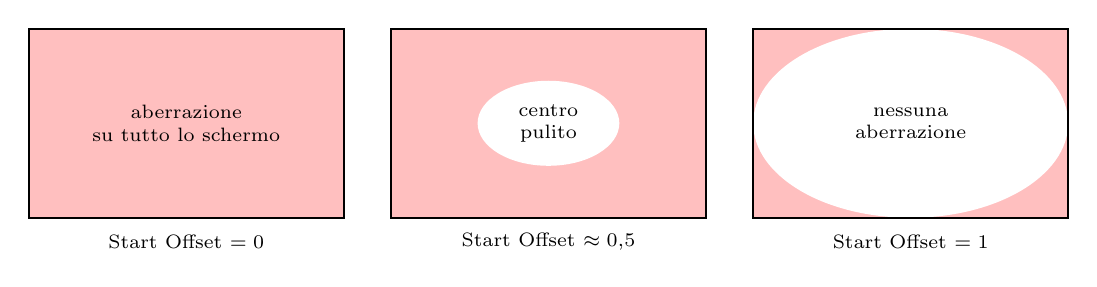
\begin{tikzpicture}[font=\scriptsize, x=1cm, y=1cm]
  \foreach \xs/\r/\lab in {0/0.0/{Start Offset $=0$}, 4.6/0.9/{Start Offset $\approx 0{,}5$}, 9.2/2.0/{Start Offset $=1$}} {
    \begin{scope}[xshift=\xs cm]
      \begin{scope}
        \clip (0,0) rectangle (4,2.4);
        \fill[red!25] (0,0) rectangle (4,2.4);
        \fill[white] (2,1.2) ellipse ({\r} and {\r*0.6});
      \end{scope}
      \draw[thick] (0,0) rectangle (4,2.4);
      \node at (2,-0.3) {\lab};
    \end{scope}
  }
  \node[align=center] at (2,1.2) {aberrazione\\su tutto lo schermo};
  \node[align=center] at (6.6,1.2) {centro\\pulito};
  \node[align=center] at (11.2,1.2) {nessuna\\aberrazione};
\end{tikzpicture}
\caption{Lo Start Offset della Chromatic Aberration: dal centro dello schermo fino al valore
impostato l'immagine resta pulita, oltre compare la separazione dei canali. A 1 l'effetto
sparisce. Ricostruzione schematica.}
\label{ue16:fig:chromatic}
\end{figure}

\paragraph{Approfondimento: aberrazione e accessibilità.} L'aberrazione cromatica imita un
difetto degli obiettivi reali, che non fanno convergere nello stesso punto le diverse
lunghezze d'onda: per questo è più forte ai bordi. Il consiglio del docente coincide con una
pratica diffusa dell'accessibilità: effetti come aberrazione, motion blur, vignettatura forte e
\emph{film grain} affaticano la vista o danno nausea a una parte dei giocatori, e molti giochi
offrono un'opzione per disattivarli. In Unreal si può farlo modificando a runtime le proprietà
del post process (per esempio il \emph{Post Process Settings} di una camera o di un volume da
Blueprint) oppure, per un picco di breve durata come la flashbang, animando l'intensità con una
\emph{Timeline}, lo strumento visto nelle prime lezioni del corso (funzionamento generale
dell'engine). Totten, nel capitolo 5, ricorda che l'horror lavora sull'incertezza percettiva
(l'ombra, la nebbia): l'aberrazione dell'esempio lovecraftiano è la versione
``sullo schermo'' della stessa strategia.

% ---------------------------------------------------------------------
\section{Il Lens Flare}
\label{ue16:sec:flare}

\paragraph{Che cos'è.} ``Questa è un'altra molto comune, molto vista'': ``forse è il tipo di
post-process con cui siamo più familiari'', perché si vede spesso anche nelle immagini delle
fotocamere. È la ``scomposizione dello spettro della luce'': dentro il volume la luce viene
scomposta, e si vedono ``gli esagoni che si creano''. Si può usare ``per diecimila motivi'':
per esempio quando il personaggio è appena uscito all'aperto dopo essere stato al chiuso, e la
scomposizione ``ci accoglie e ci dà un'idea di quanto effettivamente il sole sia forte'', o una
luce in generale.

\paragraph{I parametri.}
\begin{itemize}
  \item \textbf{Intensity}: quanto è forte. ``Se non ricordo male'' è influenzato anche dal
        \textbf{bloom}: ed ``esatto'', aumentando l'intensità del bloom il lens flare diventa
        più sfumato.
  \item \textbf{Tint}: il colore del flare, ``magari prendiamo questo flare violaceo''; si
        può anche modificare a mano il riferimento dei canali RGB.
  \item \textbf{Bokeh Size} (``poke size'': ``sono ignorante su come si pronuncia''): la
        grandezza di ``non lo so neanche come chiamarli, dei cristalli, degli esagoni della
        scomposizione della luce'', per un effetto più o meno scomposto (il docente toglie il
        blu per farlo vedere meglio).
  \item \textbf{Threshold}: ``funziona sempre nello stesso modo'', la soglia minima di
        luminosità per avere l'effetto.
  \item \textbf{Bokeh Shape}: ``devo essere onesto, non ho mai trovato un'utilità a questa
        cosa'', ma si può cambiare la forma dei cristalli con una \textbf{texture}. Quella di
        default si chiama, nella trascrizione, ``Presize default all''; cambiandola si hanno
        cerchi, pentagoni, ``qualsiasi texture abbiamo'': l'icona di un bersaglio, ``un'immaginina
        con delle stelline''. Le texture troppo dettagliate non rendono (``non si nota
        effettivamente il dettaglio''), ma per una questione di forma funzionano; la texture
        porta con sé anche il colore.
  \item \textbf{Tints}: per personalizzare ``al 100\%'' il flare, si può modificare ``ogni
        singolo cristallino'': ce n'è uno viola, uno blu, uno verde, e si decide quali colori
        dello spettro ``risultano maggiormente''. Sono numerati da 0 a 7 (la trascrizione elenca
        ``0, 1, 2, 3, 4, 5, 7'').
\end{itemize}
``Il lens flare lo teniamo, che insomma è piacevole averlo.''

\paragraph{Approfondimento: un difetto che diventa linguaggio.} Il lens flare è un riflesso
interno fra le lenti di un obiettivo, e i suoi esagoni hanno la forma del diaframma; in
Unreal Engine~5 il lens flare del post process è un effetto \emph{image-based}, calcolato a
partire dalle zone più brillanti dell'immagine (per questo dipende dal bloom e dalla soglia),
e la \emph{Bokeh Shape} è appunto la sagoma del diaframma simulato. Nel cinema e nei giochi il
flare comunica ``guardi verso una luce forte'' e, spesso, ``stai guardando attraverso una
camera'': usato ovunque, indebolisce l'idea di una visione in prima persona; usato al momento
giusto, come l'uscita all'aperto del docente, è un segnale di passaggio. Funzionamento generale
dell'engine.

% ---------------------------------------------------------------------
\section{La Depth of Field}
\label{ue16:sec:dof}

\paragraph{Mettere a fuoco.} ``Un'altra cosa molto importante che possiamo utilizzare nel
momento in cui andiamo a fare un render di un'immagine, ma anche quando dobbiamo gestire le
distanze'', è la \textbf{Depth of Field} (la profondità di campo). Permette ``una serie di
modifiche di messa a fuoco'': si modifica la \textbf{distanza focale}, cioè a quale distanza si
mette a fuoco. Nella prova c'è ``una leggera sfocatura'', e più in là ``qualcosa di meno messo a
fuoco, ma comunque non visibilissimo'': ``mettiamo che il nostro personaggio sia vagamente
miope, insomma, vedrà in questo modo qui''.

\paragraph{Gli altri parametri.} Il docente ricorda altri parametri che permettono di
determinare ``la distanza a cui vediamo il blur e l'intensità del blur'': ``quale sia la forza
della sfocatura e da quale distanza venga effettivamente attivata''. Ma ``ricordo funzionasse
in maniera diversa'': ``credo che sulla 4 funzioni in maniera diversa''. Promette di
controllare durante la pausa e di riferire le eventuali modifiche; dopo la pausa, però, la
trascrizione non riporta più nulla sulla depth of field.

\paragraph{Approfondimento: la profondità di campo in Unreal Engine~5.} La differenza che il
docente ricorda c'è davvero. In Unreal Engine~4 esistevano più metodi (\emph{Gaussian},
\emph{Bokeh}, \emph{Circle}), ciascuno con parametri propri come le regioni di transizione
vicina e lontana; in Unreal Engine~5 su PC e console resta di fatto un solo metodo, il
\emph{Cinematic} DOF, i cui parametri principali sono la \emph{Focal Distance} (la distanza
di messa a fuoco, in centimetri), l'\emph{Aperture} o \emph{f-stop} della camera (più è basso,
più la profondità di campo è stretta) e la dimensione del sensore; sono presenti anche
\emph{Depth Blur km for 50\%} e \emph{Depth Blur Radius}, che aggiungono una sfocatura di
distanza indipendente dalla messa a fuoco. Il \emph{Mobile Depth of Field} che il docente vede
nella lista della Camera Actor è la versione semplificata per dispositivi mobili, con distanze
di transizione esplicite, ed è probabilmente il modello di funzionamento che ricordava. Sulla
Camera Actor (\emph{Cine Camera Actor}) la messa a fuoco si regola dalle \emph{Focus Settings},
anche in modo automatico seguendo un actor (funzionamento generale dell'engine). In un gioco
la profondità di campo è utile soprattutto per i menu, i dialoghi e le schermate, dove guida lo
sguardo verso il soggetto: è la stessa funzione che Totten, nel capitolo 7, attribuisce alla
cinematografia, ``attirare l'attenzione del giocatore'' sugli elementi che il designer vuole
fargli vedere.

% ---------------------------------------------------------------------
\section{Il Color Grading}
\label{ue16:sec:grading}

\paragraph{La cosa più famosa.} ``Forse la cosa più famosa per cui è conosciuta e utilizzata
la post-produzione'' è la \textbf{color correction}: applicare all'immagine ``un nuovo stile, un
nuovo tipo di colore'' con una serie di parametri. Il docente richiude tutte le sezioni per
vederle una per una.

\paragraph{Temperature.} ``Di base, il color grading parte dalla \textbf{temperatura}'': una
scena più calda o più fredda, da un estremo all'altro, con ``questa renderizzazione più
giallastra'' o ``completamente sbiancata e bluastra''. Poi la \textbf{tinta} (\emph{Tint}), per
spingere la scena verso il magenta o verso il verde.

\paragraph{Global, Shadows, Midtones, Highlights.} Oltre alla temperatura ci sono i parametri
``che ci permettono di fare una customizzazione più completa'': \textbf{Global},
\textbf{Shadows}, \textbf{Midtones} (``mittons'') e \textbf{Highlights}. Sono la possibilità
di fare color correction su tutta la scena (Global), solo sugli scuri, ``nelle parti più buie,
nelle ombre'' (Shadows), ``nei grigi, nei medi'' (Midtones) e ``nelle luci, nelle parti più
illuminate'' (Highlights) (figura~\ref{ue16:fig:grading}).

\paragraph{Cinque sottoparametri.} ``Funzionano tutti allo stesso modo'': ognuno ha la stessa
lista di \textbf{Saturation}, \textbf{Contrast}, \textbf{Gamma}, \textbf{Gain} e
\textbf{Offset}, da attivare con la spunta ed espandere con la freccia. Con la saturazione si
decide quanto la scena sia satura o desaturata, con lo slider sotto. (A questo punto la
trascrizione si perde per diverse righe in un blocco ripetuto senza senso; quando riprende, il
docente sta parlando del \textbf{contrasto}.) Con il contrasto si gioca sulla differenza ``fra
le luci e le ombre'': la si può accentuare o appiattire, ``una sorta di maschera di contrasto
del colore''. ``Stessa cosa gamma e gain'': moltiplicano la color correction della scena, e si
alzano o abbassano per modificare il colore.

\begin{figure}[htbp]
\centering
\begin{tikzpicture}[font=\scriptsize, x=1cm, y=1cm]
  \shade[left color=black, right color=white] (0,0) rectangle (12,0.7);
  \draw[thick] (0,0) rectangle (12,0.7);
  \draw[thick] (0,1.0) -- (4,1.0);
  \node at (2,1.3) {\textbf{Shadows}: ombre};
  \node at (6,1.3) {\textbf{Midtones}: grigi, medi};
  \node at (10,1.3) {\textbf{Highlights}: luci};
  \draw[thick] (4,0) -- (4,1.1); \draw[thick] (8,0) -- (8,1.1);
  \draw[thick, {Stealth[length=1.6mm]}-{Stealth[length=1.6mm]}] (0,1.8) -- (12,1.8) node[midway, above] {\textbf{Global}: tutta la scena};
  \node[align=center, draw, rounded corners=2pt, fill=gray!10, inner sep=4pt] at (6,-0.9)
    {in ognuna: Saturation $\cdot$ Contrast $\cdot$ Gamma $\cdot$ Gain $\cdot$ Offset};
  \node[align=center, draw, rounded corners=2pt, fill=orange!10, inner sep=4pt] at (6,-1.8)
    {prima, per tutta l'immagine: Temperature (caldo / freddo) e Tint (magenta / verde)};
\end{tikzpicture}
\caption{Le zone del Color Grading. Global agisce su tutta l'immagine, Shadows, Midtones e
Highlights sulle zone scure, medie e chiare; ciascuna ha gli stessi cinque sottoparametri.
I confini fra le zone sono sfumati e regolabili. Ricostruzione schematica.}
\label{ue16:fig:grading}
\end{figure}

\paragraph{Uno strumento avanzato.} ``Il post-process è un elemento molto molto avanzato'':
non perché sia difficile da usare, ``ma nel senso che è difficile ottenere esattamente il
risultato che volete''. È un oggetto con cui ``dovete sperimentare, mettervi là, fare
esperienza'' di come funziona e di quali possibilità ha. ``Se dovessimo esplorarlo al 100\%
ci vorrebbe molto di più di una lezione, e probabilmente non sarei neanche la persona adatta.''
Il docente ha mostrato le lenti ``che potreste utilizzare di più'' per creare un certo
\emph{mood} e un certo tipo di scena; si ferma qui per parlare di altre cose ``ugualmente
importanti'', ``più basilari forse, meno avanzate''. Chi vuole può partire da questa base:
mettere in scena il proprio post process e ``smontarlo un pochino''.

\paragraph{Prima le luci, poi il post process.} La post produzione ``influisce grandemente
sulla luce'': a seconda del tipo di luce in scena si avranno effetti diversi. L'ordine giusto:
prima si costruisce l'illuminazione, ``come abbiamo visto con i light actor qualche lezione
fa'', e solo quando le luci sono posizionate si fa questo lavoro. ``Capisco che è stato molto
brutale e molto rapido'', ma ``più che mostrarvi gli elementi di base e incitarvi a provare a
sperimentare'' non c'è tempo. ``Oggi purtroppo corriamo un po'.''

\paragraph{Approfondimento: colore e significato.} Il color grading di Unreal segue il
modello dei programmi di correzione colore del cinema: Saturation, Contrast, Gamma, Gain e
Offset sono i classici controlli di \emph{lift-gamma-gain} applicati per zone, e i confini
fra Shadows, Midtones e Highlights si regolano con \emph{Shadows Max} e \emph{Highlights Min};
per un controllo totale si può usare una \emph{Color Grading LUT}, una tabella di colori
preparata in un programma esterno (funzionamento generale dell'engine). Totten, nel capitolo 4
(``Basic Color Theory''), fornisce il vocabolario per scegliere: i colori \emph{analoghi}
(tre colori vicini sulla ruota, come blu, blu-viola e viola) creano un'atmosfera armonica e,
in quel caso, ``un senso cupo o freddo''; rosso, rosso-arancio e arancio danno una sensazione
calda; i \emph{complementari} (opposti sulla ruota) creano contrasto. È esattamente il
``posto lugubre'' del docente, caricato di verdi, blu e viola. L'esempio di Totten è
\emph{Bioshock Infinite}: una cappella dominata dal blu in cui le uscite sulla strada
principale sono segnate da elementi complementari, una luce arancione o un fedele in tunica
bianca, mentre i passaggi secondari restano in tinte analoghe. Il color grading regola il
colore dominante; il contrasto che guida il giocatore va poi costruito con le luci e gli
oggetti.

% ---------------------------------------------------------------------
\section{La domanda sull'effetto in due toni}
\label{ue16:sec:duetoni}

\paragraph{La domanda.} Prima di passare al packaging arriva una domanda in chat: ``si possono
applicare effetti di luce più estremi, magari su altri programmi?'' Per esempio ``rendere il
livello in due toni'', ``solo rosso e nero'', per ottenere ``un effetto tipo
\textbf{Limbo}''. ``Sì, si può fare, ma anche già soltanto all'interno di Unreal, utilizzando
un post process volume.''

\paragraph{La zanzara e il cannone.} Il docente sposta però la questione: non è tanto ``se
Unreal lo può fare oppure no'', ma ``per fare quella cosa, è davvero necessario utilizzare
Unreal?'' Se l'idea è creare qualcosa di esteticamente molto semplice, in bianco e nero, si
può forse realizzarlo con altri engine. ``Teniamo sempre a mente che Unreal è un engine pesante
che fa le cose in maniera pesante.'' Se si vuole rifare Limbo, ``che magari è anche in 2D'' e
quindi più semplice, e lo si fa in Unreal, ``stiamo sparando a una zanzara con un cannone'':
``la zanzara l'ammazziamo, però smontiamo pure quello che c'è dietro''. Quanto agli ``altri
programmi'': se si fa un'immagine in Unreal, uno screenshot di un ambiente, e la si modifica
``in post'' con un programma di fotoritocco, ``sì, lo posso fare''.

\paragraph{Mallory.} Lo studente cita un gioco, ``Mallory'' (``Mellori'' più avanti; il nome
esatto non è ricostruibile dalla trascrizione), un titolo per Switch fatto in Unreal, e
condivide dei link. Il docente non lo conosce: ``poi me lo guardo durante la pausa''. In ogni
caso, ``se è fatto in Unreal si può fare tranquillamente'': l'idea stessa del Post Process
Volume è avere un oggetto in scena che permette di passare da un tipo di post produzione a un
altro o di controllarla meglio; ``una volta che mi impratichisco con lo strumento posso fare
un po' quello che mi pare''. Serve però anche gestire bene l'illuminazione: ci si costruisce
l'illuminazione ``come è gestita in quel titolo'' e poi la si modifica a posteriori. (Il
seguito, dopo la pausa, è nella sezione~\ref{ue16:sec:pausa}.)

\paragraph{Approfondimento: scegliere l'engine.} La metafora del cannone tocca un tema di
produzione: il costo di un engine non è solo la licenza, ma il peso dei progetti, i tempi di
compilazione degli shader e del packaging (che il docente sperimenterà di lì a poco) e le
macchine richieste ai giocatori, come ha scoperto lo studente con il portatile che ``non
reggeva''. Per un gioco 2D stilizzato un engine più leggero è spesso la scelta più efficiente;
Unreal ha comunque strumenti 2D (\emph{Paper2D}, gli sprite e i flipbook citati nella lezione
precedente). Un effetto ``in due toni'' in Unreal si ottiene con un \emph{Post Process
Material}: un materiale con dominio \emph{Post Process}, assegnato nei \emph{Rendering
Features} del volume (\emph{Post Process Materials}), che legge il colore della scena e lo
riduce a due colori secondo una soglia di luminosità (funzionamento generale dell'engine).
Totten, nel capitolo 4, usa proprio \emph{Limbo} come esempio di linguaggio visivo: il gioco
gioca il suo stile a silhouette contro le convenzioni del giocatore, come nel puzzle della
pressa in cui il ``pulsante'' rialzato non è il vero meccanismo. Lo stile in due toni, lì, non
è un filtro sopra il gioco: è parte delle regole con cui il giocatore legge lo spazio.

% ---------------------------------------------------------------------
\section{Il packaging: che cos'è e dove si avvia}
\label{ue16:sec:packaging}

\paragraph{Che cos'è.} ``Il packaging è un processo che viene fatto principalmente da Unreal
Engine, in realtà, per cui noi dobbiamo andare a curare soltanto alcune impostazioni.'' È ciò
che ``ci consente di andare a creare un \textbf{eseguibile} con quello che noi abbiamo
all'interno dell'editor''.

\paragraph{Platforms.} Il packaging si avvia dal pulsante \textbf{Platforms} della barra degli
strumenti. Scendendo si vedono ``tutte le varie piattaforme per cui potremmo sviluppare
qualcosa'': \textbf{Android}, \textbf{iOS}, \textbf{Linux}, \textbf{Mac}, \textbf{Windows}.
Accanto ad alcune c'è ``sempre questo segnale di attenzione'': il docente è su Windows, e il
progetto ``non è gestito o pensato'' per funzionare anche sugli altri sistemi. Nella voce
\textbf{Windows} ci sono il \textbf{Package Project}, ``il pulsantone che io premo se voglio far
partire questo processo'', e la scelta della \textbf{configurazione}. ``Queste sono pochissime
impostazioni, e non sono neanche lontanamente tutte quelle che ci servono'': le altre sono nei
\textbf{Project Settings}, la ``macro sezione di setting e di impostazioni per tutto il nostro
progetto'' già vista con Igor (figura~\ref{ue16:fig:packaging}).

\paragraph{Il plugin di Fab.} Un'altra finestra che può servire è quella dei \textbf{Plugins},
che permette di attivare e disattivare i plugin. ``Da quello che so, il plugin di
\textbf{Fab} dà dei problemi con il packaging'': quindi, prima di impacchettare, lo si
disattiva. ``Non so se è stato risolto. Potrebbe essere stato risolto, dovrei informarmi.''

% ---------------------------------------------------------------------
\section{Le impostazioni del progetto}
\label{ue16:sec:impostazioni}

\paragraph{Maps \& Modes.} Nei Project Settings, nella pagina \textbf{Maps \& Modes}, ``oltre
alla Game Mode'', ci sono le \textbf{Default Maps}: \textbf{Editor Startup Map} e
\textbf{Game Default Map}.
\begin{itemize}
  \item L'\textbf{Editor Startup Map} è la mappa con cui si apre l'editor: se la si cambia,
        ``ogni volta che io aprirò questo progetto lui mi partirà da quell'altra mappa'', e per
        tornare al livello di prima bisognerà riaprire a mano la Third Person Map.
  \item La \textbf{Game Default Map} è ``allo stesso modo la mappa di partenza che avremo
        all'interno del nostro eseguibile''. Se il gioco ha un menu che porta alla mappa di
        gioco, non si mette la Third Person Map: ``di solito quello che si fa è mettere un
        \textbf{menu principale}'', o una schermata che, dopo aver cliccato qualche pulsante,
        porta alle mappe che si vogliono giocare.
\end{itemize}
Sono due impostazioni importanti: ``se mai vi capiterà di dire: oddio, dove è andata la mia
mappa, perché si è aperto così, dove sono finito, cosa è successo''; oppure ``per quale motivo
ho fatto il packaging e non mi fa partire da dove dico io'': è la Game Default Map da
modificare. (Il docente scorre altre voci della pagina, ``ma questa non è necessaria'', senza
nominarle.)

\paragraph{Supported Platforms.} Un'altra pagina è quella delle \textbf{Supported Platforms}.
Di default è impostata su \textbf{All Platforms}; togliendo la spunta e lasciando solo ciò che
interessa si può avere, per esempio, soltanto \textbf{Windows} come piattaforma per il
packaging, ``perché il nostro progetto magari non supporta tutti gli altri sistemi
operativi''.

\paragraph{La pagina Packaging.} ``Ultima cosa, ma la più importante'': c'è una pagina tutta
dedicata al \textbf{packaging}. ``Sono un sacco di informazioni, un sacco di parametri'', ma
``la cosa positiva è che la maggior parte di questi parametri sta bene come sta'': non servono
``modifiche assurde''. Alcune voci si vedono subito, altre solo aprendo gli
\textbf{Advanced}. Le prime: \textbf{Build}, ``va bene così'' (l'opzione ``if project has code
or running a locally built editor'', che lascia decidere all'engine se compilare); poi la
\textbf{Build Configuration}.

% ---------------------------------------------------------------------
\section{Le configurazioni di build}
\label{ue16:sec:build}

\paragraph{Cinque configurazioni, tre disponibili.} La \textbf{Build Configuration} decide
``che tipo di configurazione avrà il nostro eseguibile'': \textbf{Debug}, \textbf{DebugGame},
\textbf{Development}, \textbf{Test} e \textbf{Shipping}. ``Per la build che abbiamo scelto''
ne sono attive soltanto tre (le stesse che si ritrovano poi nel menu Platforms: DebugGame,
Development e Shipping). Le differenze (tabella~\ref{ue16:tab:build}):
\begin{itemize}
  \item \textbf{Debug} e \textbf{DebugGame} ``sono modalità di debug'': un eseguibile in cui
        c'è ancora una \textbf{console di comandi} per inserire comandi, fare aggiustamenti,
        ``vedere le linee, vedere quello che sta succedendo, vedere dei text che vengono
        printati''. ``È una versione super di test.''
  \item \textbf{Development} è ``la configurazione di default di Unreal''. Rimuove la maggior
        parte della struttura di debug, aumenta un po' l'ottimizzazione della build, ``ma
        mantiene comunque alcuni strumenti che possono essere utilizzati per il testing''. ``Se
        debug è un eseguibile che può essere di uso a un \textbf{programmatore}, development può
        essere di uso a un \textbf{designer}'': si può ancora modificare qualcosa e usare degli
        input, ma serve soprattutto per testare e poi ritoccare in engine.
  \item \textbf{Shipping} è la modalità ``per la distribuzione'': ``il progetto finito, il
        gioco che le masse giocheranno, si spera le masse''. È ``la versione più ottimizzata
        possibile della build'', ``la build da vendita, praticamente''.
\end{itemize}

\paragraph{Shipping non ottimizza da solo.} ``Aspettate: questo non vuol dire che lui vi
ottimizzi le cose in automatico.'' L'ottimizzazione ``è tutto un discorso a parte, che va fatto
separatamente'': far sì che non ci siano troppe linee di codice, che non ci siano texture a
qualità troppo alta o non utilizzate, eccetera. Shipping ``vuol dire semplicemente che lui va a
togliere tutta una serie di strumenti che non servono più''.

\begin{table}[htbp]
\centering
\small
\begin{tabular}{@{}p{2.3cm}p{5.6cm}p{3.0cm}p{3.1cm}@{}}
\toprule
\textbf{Configurazione} & \textbf{Che cosa contiene (lezione)} & \textbf{Per chi} &
\textbf{Nota} \\
\midrule
Debug & console di comandi, linee, testi stampati: ``versione super di test'' &
programmatore & richiede un progetto con codice C++ \\
DebugGame & come sopra, debug del codice di gioco & programmatore & disponibile \\
Development & default di Unreal; meno debug, un po' più ottimizzata, alcuni strumenti di test
& designer, tester & disponibile; console attiva \\
Test & vicina a Shipping, con qualche strumento di profilazione & QA & richiede codice C++ \\
Shipping & la versione finale, senza strumenti di sviluppo & i giocatori & disponibile; non
ottimizza da sola \\
\bottomrule
\end{tabular}
\caption{Le cinque configurazioni di build. Nel progetto del docente ne sono attive tre; la
colonna ``Nota'' integra con il funzionamento generale dell'engine.}
\label{ue16:tab:build}
\end{table}

\paragraph{Le lingue.} Aprendo gli Advanced si trovano le \textbf{lingue} del packaging
(\emph{Localizations to Package}): ``possiamo andare a selezionare che tipo di lingue dovranno
essere utilizzate''. ``Di default c'è solo l'inglese.'' Se si è localizzato qualcosa, per
esempio perché ci sono già impostazioni e parametri che fanno riferimento a certe lingue, qui
si scelgono quelle da includere.

\paragraph{Approfondimento: le configurazioni secondo Romero e Sewell.} Romero e Sewell, nel
capitolo 12 (``Building and Publishing''), descrivono lo stesso percorso: \emph{Platforms}
$\rightarrow$ piattaforma $\rightarrow$ \emph{Package Project}, la scelta della cartella, la
finestra che avvisa che l'engine sta impacchettando e, in caso di problemi, ``i dettagli
dell'errore nella finestra dell'output log''. Prima, nei \emph{Project Settings}: la pagina
\emph{Description} (nome, miniatura, descrizione del progetto), la pagina \emph{Maps \& Modes}
(``spesso dovrete designare una mappa dedicata al menu principale come prima mappa da
caricare'', e assicurarsi che sia lei a gestire quale mappa si carica dopo) e la pagina della
piattaforma, dove per Windows si cambiano lo \emph{splash screen} e l'\emph{icona}
dell'eseguibile. Sulle configurazioni il libro precisa che nei progetti \emph{solo
Blueprint} le opzioni principali sono \textbf{Development}, che contiene informazioni di debug
utili a trovare errori, e \textbf{Shipping}, ``più pulita'', da usare per la versione da
distribuire; Debug e Test richiedono un progetto con codice C++ (ed è per questo che nel
progetto del docente sono spente). Il libro nomina anche la \emph{Staging Directory}, la
cartella in cui viene salvata la build, l'opzione \emph{For Distribution}, richiesta per
pubblicare su App Store o Google Play, e lo \emph{Zip Project} del menu File, che comprime i
file essenziali del progetto per passarlo a un'altra persona. Una nota importante dello stesso
capitolo: Unreal Engine~5 può creare build Windows solo da Windows e build macOS solo da macOS;
è il ``segnale di attenzione'' che il docente vede accanto alle altre piattaforme.

% ---------------------------------------------------------------------
\section{Le mappe e le cartelle da cucinare}
\label{ue16:sec:cook}

\paragraph{Cook only maps.} ``Fare il packaging di base vuol dire che lui prende tutto il
progetto e lo rende pronto per essere un eseguibile'', con un certo metodo di compressione.
Spuntando \textbf{Cook only maps} (``hook only maps'' nella trascrizione), invece, il
packaging usa ``unicamente le mappe'': si può dirgli di usare soltanto la Third Person Map, e
lui ``si vede cosa c'è dentro'', mette nel pacchetto ``tutto quello che serve per far funzionare''
quella mappa ``e non mette il resto delle cose''.

\paragraph{List of maps to include.} Insieme a Cook only maps serve la voce \textbf{List of maps
to include in a packaged build}. Si aggiunge un elemento, si clicca sui tre puntini e si cerca
la mappa: ``volete level 1, level 2, menu? Magari vi serve il menu''. Nel caso della prova
serve soltanto la Third Person Map (il file \texttt{.umap}): ``non serve andare a inserire anche
il build data'' (il file \texttt{\_BuiltData}) ``o lo \texttt{.uasset}''. Si possono aggiungere
altre mappe, copiarle, eliminarle.

\paragraph{Directories to never cook.} ``Un'altra cosa che ci torna utile'' è
\textbf{Directories to never cook}: le cartelle che non devono mai finire nel pacchetto. Si
aggiunge un elemento (``un index zero'') e si sceglie la cartella. Gli esempi:
\begin{itemize}
  \item ``nulla di \emph{GameApps}'' (il nome della cartella, nella trascrizione, è ``game
        apps'') ``deve finire dentro il packaging'';
  \item una cartella con ``tutta una serie di modelli 3D molto fighi'' che non si è riusciti a
        inserire e che magari si vogliono usare in un \textbf{DLC} più avanti.
\end{itemize}
I motivi sono due. Il primo è il \textbf{data mining}, ``diventato super popolare adesso'': i
file messi nel gioco ``possono essere ritrovati da chi va a scavare''. Il secondo: sono comunque
cose ``che vanno ad essere cucinate e vengono comunque inserite all'interno della build''.
Togliere le cartelle che non servono ``ci fa risparmiare giga'': un progetto più piccolo e più
semplice da gestire (tabella~\ref{ue16:tab:packaging}).

\begin{table}[htbp]
\centering
\small
\begin{tabular}{@{}p{4.6cm}p{2.8cm}p{6.6cm}@{}}
\toprule
\textbf{Impostazione} & \textbf{Dove} & \textbf{A che cosa serve} \\
\midrule
Package Project, configurazione & Platforms $\rightarrow$ Windows & avviare il packaging;
scegliere DebugGame, Development, Shipping o le impostazioni del progetto \\
Plugin di Fab & Edit $\rightarrow$ Plugins & disattivarlo prima del packaging (problemi
noti, forse risolti) \\
Editor Startup Map & Maps \& Modes & la mappa con cui si apre l'editor \\
Game Default Map & Maps \& Modes & la prima mappa dell'eseguibile: di solito il menu \\
Supported Platforms & Project Settings & limitare le piattaforme (per esempio solo Windows) \\
Build & Packaging & lasciare il default \\
Build Configuration & Packaging & Debug, DebugGame, Development, Test, Shipping \\
Localizations to Package & Packaging (Advanced) & le lingue incluse; default inglese \\
Cook only maps & Packaging (Advanced) & impacchettare solo ciò che serve alle mappe elencate \\
List of maps to include & Packaging (Advanced) & le mappe (\texttt{.umap}) da includere \\
Directories to never cook & Packaging (Advanced) & cartelle escluse: asset scartati, DLC,
spazio \\
Show Output Log & finestra del packaging & seguire il processo e trovare gli errori in rosso \\
\bottomrule
\end{tabular}
\caption{Le impostazioni del packaging viste a lezione, nell'ordine in cui il docente le
mostra.}
\label{ue16:tab:packaging}
\end{table}

\paragraph{Approfondimento: che cosa vuol dire ``cucinare''.} Il \emph{cooking} è la fase in
cui l'engine converte gli asset dal formato dell'editor a quello ottimizzato per la
piattaforma di destinazione: compila gli shader, comprime le texture, elimina i dati che
servono solo all'editor. Il packaging vero e proprio raccoglie poi gli asset cucinati in
archivi (\emph{.pak}, o \emph{IoStore} in Unreal Engine~5) accanto all'eseguibile. Con Cook
only maps disattivato l'engine cucina di norma tutto il contenuto del progetto, compresi gli
asset mai usati; con l'opzione attiva segue le \emph{reference} a partire dalle mappe
elencate. Un'avvertenza: un asset caricato solo per nome, a runtime (per esempio con un
percorso scritto in una stringa), non è una reference visibile al cook e rischia di restare
fuori; per questi casi esistono le voci \emph{Additional Asset Directories to Cook}. Anche
\emph{Directories to never cook} va usata con attenzione: se un asset escluso è referenziato
da una mappa inclusa, il cook segnala un errore o il gioco lo perde (funzionamento generale
dell'engine). Totten, nel capitolo 2, parla di \emph{modular design} e di ``schedule'' dei
pezzi di un livello: sapere fin dalla pre-produzione quali pezzi servono rende più facile
anche sapere, alla fine, che cosa lasciare fuori.

% ---------------------------------------------------------------------
\section{L'avvio del packaging e l'Output Log}
\label{ue16:sec:avvio}

\paragraph{Dove salvare.} Per avviare si torna al menu Platforms: lì si vedono le
configurazioni (``debug'', \textbf{Development} e \textbf{Shipping}, ``perché sono le tre
possibili''), oppure \emph{Use Project Setting}, cioè quelle della pagina Packaging. Il docente
sceglie \textbf{Development}. Con \textbf{Package Project} si apre una finestra che chiede dove
creare il pacchetto; il docente sceglie il desktop, e parte il processo, accompagnato da un
``suonino''.

\paragraph{La prima volta è lenta.} ``Fare un packaging la prima volta è molto lento'', anche
se è solo di una mappa. ``Dopo il primo packaging diventa tutto molto più veloce.'' Mentre
lavora (``parte \emph{Cancel}, chiaramente'', per interromperlo) si può aprire lo
\textbf{Show Output Log}: lì si vede tutto quello che sta succedendo. Scorrendolo (``con la
rotella del mio mouse che è rotta è tremendo'') si controlla se va tutto bene, se ci sono
errori o ``piccoli problemi'', o cose che creano problemi al packaging. In quel momento
l'engine sta facendo ``la compilazione degli shader''.

\paragraph{La scritta rossa.} ``Arriverà un punto in cui magari c'è una scritta rossa.'' La
scritta rossa ``vuol dire che c'è un problema che gli impedisce di fare il packaging''. Si legge
che cosa dice, si risolve quel problema, e si riprova.

\paragraph{Che cosa esce.} Se il processo finisce, nella cartella scelta si crea una cartella
che, ``se non gli viene dato un nome'', si chiama \textbf{Windows No Editor} (in Unreal
Engine~5 è semplicemente \emph{Windows}; \emph{WindowsNoEditor} era il nome di Unreal
Engine~4). Dentro c'è l'\textbf{eseguibile}: avviandolo parte il progetto, che in questo caso
sarebbe soltanto la Third Person Map, ``perché è l'unica mappa che gli abbiamo detto di
cucinare''. Il personaggio spawna sul \textbf{Player Start} e può andare in giro: ``non c'è un
obiettivo, non c'è una fine, non c'è nulla''.

\paragraph{I confini della mappa.} ``Chiaramente, per un packaging, non dovrebbero esserci
posti in cui puoi buttarti di sotto nel nulla, come il bordo della mappa''; né posti ``in cui
io non voglio che i giocatori vadano''. Nessuna domanda sul packaging. Siccome ci vorrà ``un
po' troppo tempo'', il docente anticipa la pausa, ``in modo che forse durante la pausa lui
finisca di calcolare'' e si possa vedere che cosa genera. Dopo la pausa: ``un paio di altri
attori'' utili quando si fa un livello, il Blueprint delle \textbf{spline}, ``che potete
utilizzare per un sacco di elementi diversi'', e, ``se ci avanza un po' di tempo'', le
\textbf{decal}, ``un altro strumento di decoro, di arredo'' per aggiungere dettagli in giro per
la mappa. ``Facciamo un 15 minuti di stop. Ci rivediamo alle 5 e mezza.''

\begin{figure}[htbp]
\centering
\begin{tikzpicture}[font=\scriptsize, x=1cm, y=1cm,
  ue16step/.style={draw, thick, rounded corners=2pt, fill=white, align=center, text width=2.6cm, minimum height=1.1cm, inner sep=3pt},
  ue16arr/.style={-{Stealth[length=1.8mm]}, thick}]
  \node[ue16step, fill=gray!10] (a) at (0,0) {Plugins:\\disattivare Fab};
  \node[ue16step, fill=blue!8] (b) at (3.3,0) {Maps \& Modes:\\Game Default Map\\(il menu)};
  \node[ue16step, fill=blue!8] (c) at (6.6,0) {Packaging:\\configurazione,\\lingue, mappe,\\cartelle escluse};
  \node[ue16step, fill=orange!12] (d) at (9.9,0) {Platforms $\rightarrow$\\Windows $\rightarrow$\\Package Project};
  \node[ue16step, fill=red!8] (e) at (9.9,-2.2) {Output Log:\\shader, cook;\\scritte rosse?};
  \node[ue16step, fill=green!12] (f) at (6.6,-2.2) {cartella \emph{Windows}\\con l'eseguibile};
  \node[ue16step, fill=green!12] (g) at (3.3,-2.2) {ritestare il gioco\\impacchettato};
  \node[ue16step, fill=green!12] (h) at (0,-2.2) {caricare (itch.io,\\Drive) e link\\su Discord};
  \draw[ue16arr] (a) -- (b); \draw[ue16arr] (b) -- (c); \draw[ue16arr] (c) -- (d);
  \draw[ue16arr] (d) -- (e); \draw[ue16arr] (e) -- (f); \draw[ue16arr] (f) -- (g);
  \draw[ue16arr] (g) -- (h);
  \draw[ue16arr, red!70!black] (e.east) -- ++(0.6,0) |- node[pos=0.25, right, align=left] {errore:\\risolvere\\e ripartire} (d.east);
\end{tikzpicture}
\caption{Il percorso del packaging come emerge dalla lezione, fino al consiglio finale di
ritestare il gioco impacchettato e condividerlo. Ricostruzione schematica.}
\label{ue16:fig:packaging}
\end{figure}

% ---------------------------------------------------------------------
\section{La pausa e Mallory}
\label{ue16:sec:pausa}

\paragraph{Il packaging non finisce.} Durante la pausa la trascrizione contiene soltanto il
blocco ripetuto già visto, che non appartiene alla lezione. Alla ripresa: ``purtroppo noi ci
siamo, ma Unreal ancora no, ancora non ho finito col packaging''. Il docente lo interrompe,
``perché sennò mi impedisce di fare altre robe'': ``non pensavo ci volesse così tanto tempo''.
Il risultato del packaging, quindi, non viene mostrato.

\paragraph{Mallory, visto.} Il docente ha guardato il gioco segnalato prima. ``Sembra molto
carino'': non l'ha potuto giocare, ma dal video ``sembra un platform simpatico con un bell'ambiente''.
Non gli è sembrato che ci sia ``un eccessivo utilizzo del post-process''. Quello che fanno
``sicuramente'' è cambiare il modo in cui vengono renderizzate luci e ombre: ``ci sono delle parti
con le ombre che sono molto rossastre rispetto alla luce, che magari è una luce più neutra'',
``una piccola vignettatura'' e ``un effetto di sfocatura messa davanti alla camera''. Lo
studente ha in mente anche altri titoli; il docente osserva che il genere platform ``ora come ora
è messo in mano agli indipendenti'': ``non ci sono più grossi titoloni che fanno quel tipo di
roba''. È giusto cercare ``cose carine fatte da persone in giro'', su Twitch o fra i piccoli
titoli su Steam. ``Purtroppo non è proprio il mio genere'', a parte ``i vecchi classiconi PS1,
PS2''.

\paragraph{Come rifare quell'effetto.} Le indicazioni del docente:
\begin{itemize}
  \item una \textbf{Dirt Mask}, come effetto di camera: una texture sovrapposta alla lente. Fra
        le texture del progetto non ce n'è una adatta; una ``un po' più fitta'' dà già ``questa
        specie di effetto statico, tra virgolette, sulla camera'', da gestire poi con i colori
        corretti (quella provata rende la Dirt Mask rossa: ``se riesci a fartela di effetto
        statico perfetto, potrebbe non essere male'');
  \item negli \textbf{Image Effects}, una piccola \textbf{vignettatura} (\emph{Vignette
        Intensity}), che ``va a scurire lo schermo'' nelle parti esterne e dà ``già di base'' un
        mood un po' più scuro;
  \item il resto ``è tutta \textbf{color correction}'': modificare i colori delle ombre per
        avvicinarli a quelli delle luci, desaturare un po' la scena (``c'è fondamentalmente una
        scala di grigio e in più c'è il rosso, barra rosa'') e mettere ``un accento sul rosso''
        dove c'è il rosso.
\end{itemize}

\paragraph{Monument Valley.} Mallory ricorda al docente, per la struttura dei livelli ``molto
geometrici, molto quadratosi'', i \textbf{Monument Valley}: ``non sono dei platform, sono dei
puzzle game misto opera estetica''. Si basano sull'\textbf{illusione ottica}: il personaggio
``cammina su un corridoio e poi improvvisamente inizia a camminare sulla parete e poi passa
dietro la scena'', e bisogna ruotare il livello per capire dove sta andando. ``Faccio fatica a
descriverli, però cercali, sono molto carini.'' Poi si torna al programma: ``post process,
rapidamente e bruttamente, ma lo abbiamo visto''.

\paragraph{Approfondimento: accentare un colore.} L'``accento sul rosso'' in una scena
desaturata è un'applicazione diretta del contrasto di Totten (capitolo 4): un elemento di un
colore diverso dal dominante attira l'attenzione, e se il colore è sempre lo stesso diventa un
segnale che il giocatore impara a leggere. In Unreal non c'è un controllo per ``desaturare
tutto tranne il rosso'' nel color grading standard: lo si ottiene con un Post Process Material
o, più semplicemente, desaturando con il post process e dando agli oggetti rossi materiali con
un po' di \emph{emissive}, così che restino saturi anche dopo la correzione. La vignettatura si
regola con \emph{Vignette Intensity} negli \emph{Image Effects}; la Dirt Mask nella sezione
\emph{Lens}, con \emph{Dirt Mask Texture}, \emph{Intensity} e \emph{Tint}, ed è visibile solo
dove c'è bloom (funzionamento generale dell'engine). Totten, nel capitolo 4, nota anche come
le associazioni dei colori passino nei giochi: rosso e verde per la salute, blu per la magia.

% ---------------------------------------------------------------------
\section{Le spline: che cosa sono}
\label{ue16:sec:spline}

\paragraph{Una linea.} Il docente ha preparato due Blueprint ``al volo prima di cominciare la
lezione''. Prima, però, ``che cos'è una spline?'' È un \textbf{component} che si può aggiungere
ai Blueprint, ma ``in realtà è proprio un tipo di oggetto'' con una funzione ben specifica, che
si usa anche per modificare il funzionamento del \textbf{landscape} (le \emph{landscape
spline}). Il docente crea un Blueprint di prova con un \textbf{Spline Component}; il tooltip
dice che è ``una spline shape che può essere usata per altri scopi, tipo animare oggetti''.
``È una linea, fondamentalmente.''

\paragraph{Punti e tangenti.} Messa in scena, la spline ``non è nient'altro che una linea'' che
si può allungare, curvare e arricchire di punti (figura~\ref{ue16:fig:spline}):
\begin{itemize}
  \item all'inizio ha \textbf{due punti}, l'inizio e la fine;
  \item cliccando sul punto finale compaiono altri due punti, la \textbf{tangente}; spostandola,
        la spline si curva;
  \item per creare \textbf{nuovi punti} si fa come quando si copia un oggetto: sulla freccia
        del gizmo, \textbf{Alt} premuto, si trascina, ``e ho fatto una copia''; ogni punto
        nuovo curva la linea, si può alzare, spostare, fino a costruire ``una figura, una
        struttura'';
  \item con il tasto destro, \textbf{Delete Spline Point} elimina un punto (la spline si
        riempie da sola fra i punti rimasti, ``lui autofilla'') e \textbf{Add Spline Point
        Here} ne aggiunge uno.
\end{itemize}

\begin{figure}[htbp]
\centering
\begin{tikzpicture}[font=\scriptsize, x=1cm, y=1cm]
  \draw[very thick, blue!70!black] (0,0) .. controls (2,0) and (2.5,2) .. (4.5,2)
                                   .. controls (6.5,2) and (6.5,0) .. (8.5,0.3)
                                   .. controls (10,0.5) and (10.5,1.6) .. (11.5,1.8);
  \foreach \p/\n in {(0,0)/0, (4.5,2)/1, (8.5,0.3)/2, (11.5,1.8)/3} {
    \fill[white, draw=black, thick] \p circle (3pt);
    \node[below=4pt] at \p {punto \n};
  }
  % tangente sul punto 1
  \draw[thick, red!70!black, {Stealth[length=1.5mm]}-{Stealth[length=1.5mm]}] (2.9,2) -- (6.1,2);
  \fill[red!70!black] (2.9,2) circle (2pt); \fill[red!70!black] (6.1,2) circle (2pt);
  \node[above, red!70!black] at (4.5,2.1) {tangente: lunghezza e verso curvano la linea};
  \node[align=left, anchor=west] at (0,-1.1) {Alt + trascinamento su un punto: nuovo punto \quad
    tasto destro: Add Spline Point Here, Delete Spline Point};
  \node[align=left, anchor=west] at (0,-1.6) {segmenti = punti $-$ 1 (qui 4 punti, 3 segmenti: indici da 0 a 2)};
\end{tikzpicture}
\caption{Una spline con quattro punti. Ogni punto ha una posizione e una tangente; i segmenti
sono uno in meno dei punti. Ricostruzione schematica.}
\label{ue16:fig:spline}
\end{figure}

% ---------------------------------------------------------------------
\section{A che cosa servono le spline}
\label{ue16:sec:usi}

\paragraph{Il muro di spine.} ``Immaginate di poter piazzare un oggetto lungo questa linea, o
di poter modellare un oggetto lungo questa linea.'' La storia che il docente racconta gli è
successa ``quando stavo in Accademia'', quando aveva cominciato a ``smanettare con questo
strumentino''. Bisogna creare un \textbf{muro di spine}, come nella \emph{Bella addormentata
nel bosco}, ``tutte le spine attorno al castello''. Due strade:
\begin{itemize}
  \item andare dall'``amico grafico'' e chiedergli ``un muro di spine fatto così, così e così'':
        una mesh ``non particolarmente impegnativa'', ma che richiede tempo e che, se va
        modificata, deve tornare in un software di modellazione come \textbf{Blender} o
        \textbf{Maya};
  \item ``una roba un po' più intelligente'': farsi creare soltanto un \textbf{cilindro di
        spine} e \emph{replicarlo} lungo una spline, così che la mesh ``viene ricreata e viene
        modificata sulla base della spline'', seguendone l'andamento.
\end{itemize}

\paragraph{Altri usi.} ``Al di là di questa cosa'', la struttura serve per molte cose: una
\textbf{pista} per un gioco di macchine (``vi create un blueprint di spline con la strada''); un
\textbf{muro} più stondato nel blockout o nella gym, per esempio ``che sale a spirale verso
l'alto'', quando ``non avete nulla che ve lo fa fare in maniera comoda''. Il docente lo mostra
``in due forme, in due versioni'': una ``più semplice e più brutta'', l'altra ``un po' più
funzionale''. I Blueprint si chiamano \textbf{Spline by Length} e \textbf{Spline by Point}.

\paragraph{La mesh del tubo.} Per la prova usa un tubo, ``un oggetto molto semplice'' che è
anche nel progetto degli studenti: \textbf{SM\_PipeSplineBody} (``Sm pipe spline body''). Il
docente prima dice che ``non è fatto benissimo per essere un oggetto da spline'', poi si
corregge: ``ho detto una cazzata, l'avevo vista in maniera veloce prima''. Funziona bene
perché è \textbf{segmentato}: ha i suoi triangoli e ``questa spezzatura in orizzontale'', è
\textbf{modulare} (``cilindro, cilindro, cilindro''). Questo permette al Blueprint di
replicarlo ``senza andarlo a spezzare'', perché la struttura del tubo viene replicata cilindro
per cilindro. Nella prima versione, allungando la spline il cilindro si allunga; piegandola,
si piega ``però si spezza'', perché è fatta ``in una maniera meno ottimale''; nella seconda ``si
spacca'' ancora, ma ``dovrebbe notarsi di meno''. La differenza (figura~\ref{ue16:fig:pointlength}):
``il primo blueprint, by point, \emph{stretcha} l'oggetto; questo invece ricrea l'oggetto per
lunghezza, quindi è un pochino più fedele''.

\begin{figure}[htbp]
\centering
\begin{tikzpicture}[font=\scriptsize, x=1cm, y=1cm]
  % by point
  \node[anchor=west] at (0,2.9) {\textbf{Spline by Point}: una mesh per ogni segmento, stirata fino al punto successivo};
  \foreach \a/\b/\c in {0/4.2/blue!20, 4.2/6.2/green!20, 6.2/12/orange!20} {
    \draw[thick, fill=\c] (\a,1.6) rectangle (\b,2.4);
  }
  \foreach \x in {0,4.2,6.2,12} \fill[black] (\x,2.0) circle (2.2pt);
  \node at (2.1,2.0) {stirata}; \node at (5.2,2.0) {schiacciata}; \node at (9.1,2.0) {molto stirata};
  % by length
  \node[anchor=west] at (0,1.0) {\textbf{Spline by Length}: una mesh ogni \emph{Mesh Length}, sempre proporzionata};
  \foreach \i in {0,...,5} {
    \draw[thick, fill=blue!20] ({\i*2},-0.2) rectangle ({\i*2+2},0.6);
  }
  \foreach \x in {0,12} \fill[black] (\x,0.2) circle (2.2pt);
  \draw[{Stealth[length=1.4mm]}-{Stealth[length=1.4mm]}] (0,-0.45) -- (2,-0.45) node[midway, below] {Mesh Length (250)};
  \node[align=center] at (9,-0.7) {anche con due soli punti: tanti pezzi quanti\\ne stanno nella lunghezza della spline};
\end{tikzpicture}
\caption{Le due versioni del Blueprint su una spline dritta. Per punto, il numero di mesh è
uno in meno dei punti e ciascuna si deforma fino al punto successivo; per lunghezza, il numero
di mesh dipende dalla lunghezza della spline divisa per quella della mesh. Ricostruzione
schematica.}
\label{ue16:fig:pointlength}
\end{figure}

% ---------------------------------------------------------------------
\section{Il Blueprint per punto}
\label{ue16:sec:bypoint}

\paragraph{La struttura.} Nel \textbf{Spline by Point} la viewport contiene la spline e
``un oggetto che poi gli abbiamo attaccato con un nodo''; l'Event Graph è vuoto, e tutto è nel
\textbf{Construction Script}. ``È una struttura abbastanza semplice'', usabile ``tranquillamente''
per un lavoro di blockout, ``di prototipazione''. Alcune cose il docente le fa ``un po' più
veloce, perché probabilmente le avete già viste anche con Igor''. Il grafo
(figura~\ref{ue16:fig:grafopoint}):
\begin{enumerate}
  \item un \textbf{For Loop}, ``perché dobbiamo loopare un oggetto''. Il \emph{First Index} è
        \textbf{0}, ``la base dell'indice''. Il \emph{Last Index} viene dal numero di punti della
        spline, preso trascinando la spline nel grafo e usando \textbf{Get Number of Spline
        Points}; al numero si \textbf{sottrae 2}. Il motivo detto a lezione: ``sono i due punti
        che abbiamo già di base, l'inizio e la fine'', che ``non ci interessano per il
        calcolo'' (vedi l'approfondimento più sotto per la ragione esatta);
  \item dal corpo del loop, \textbf{Add Spline Mesh Component}, con ``tutta una serie di
        parametri'': soprattutto la \textbf{Static Mesh} da usare (qui SM\_PipeSplineBody), i
        materiali, \emph{Start Position}, \emph{Start Tangent}, \emph{End Position}, \emph{End
        Tangent} e il \textbf{Forward Axis};
  \item \textbf{Set Start and End}, che dà al componente l'inizio e la fine come punti di
        riferimento;
  \item \textbf{Attach Component to Component}, che attacca il componente creato al Blueprint,
        con il \textbf{Default Scene Root} come \emph{parent};
  \item due nodi \textbf{Get Location and Tangent at Spline Point}, con la spline come target:
        il primo con l'indice del loop (posizione e tangente di partenza), il secondo con
        l'indice \textbf{più 1} (``il punto successivo''), per la fine. ``In questo modo lui, fra
        punti, va a creare una replica del nostro oggetto.''
\end{enumerate}

\begin{figure}[htbp]
\centering
\begin{tikzpicture}[font=\scriptsize, x=1cm, y=1cm,
  ue16node/.style={draw, thick, rounded corners=2pt, fill=white, align=center, minimum height=0.6cm, inner sep=3pt},
  ue16fn/.style={ue16node, fill=yellow!15},
  ue16ex/.style={ue16node, fill=blue!10},
  ue16arr/.style={-{Stealth[length=1.6mm]}, thick},
  ue16data/.style={-{Stealth[length=1.4mm]}, thin, dashed}]
  \node[ue16ex] (cs) at (0,0) {Construction\\Script};
  \node[ue16ex] (loop) at (2.6,0) {For Loop\\First 0};
  \node[ue16fn] (num) at (2.6,-1.8) {Get Number of\\Spline Points $-$ 2};
  \node[ue16ex] (add) at (5.6,0) {Add Spline Mesh\\Component\\(Mesh, Forward Axis)};
  \node[ue16ex] (sse) at (8.9,0) {Set Start\\and End};
  \node[ue16ex] (att) at (11.8,0) {Attach Component\\to Component\\(parent: Root)};
  \node[ue16fn] (g1) at (6.2,-2.0) {Get Location and Tangent\\at Spline Point (Index)};
  \node[ue16fn] (g2) at (9.9,-2.0) {Get Location and Tangent\\at Spline Point (Index + 1)};
  \draw[ue16arr] (cs) -- (loop); \draw[ue16arr] (loop) -- node[above] {Body} (add);
  \draw[ue16arr] (add) -- (sse); \draw[ue16arr] (sse) -- (att);
  \draw[ue16data] (num) -- node[left] {Last Index} (loop);
  \draw[ue16data] (loop.south east) -- (g1.north west);
  \draw[ue16data] (g1.north) -- node[left, pos=0.4] {Start Pos., Tangent} (sse.south west);
  \draw[ue16data] (g2.north) -- node[right, pos=0.4] {End Pos., Tangent} (sse.south east);
\end{tikzpicture}
\caption{Il Construction Script del Blueprint \emph{Spline by Point}. Le frecce continue
sono il flusso di esecuzione, quelle tratteggiate i dati. Ricostruzione dai nodi nominati a
lezione.}
\label{ue16:fig:grafopoint}
\end{figure}

\paragraph{Il Forward Axis.} Il docente cambia la mesh con un muro modulare (cerca
``modulare'' nel Content), compila, salva, e il risultato non è quello voluto: ``lo sta
replicando'', ma non come si vorrebbe. Il motivo è il \textbf{Forward Axis}: ``qual è l'asse
frontale dell'oggetto, qual è l'asse allineato con la spline''. Per il tubo era rimasto su
\textbf{X}, ed era giusto: aprendo la mesh, il gizmo mostra che il tubo è allineato con l'asse
X (``Z sono verticali, l'asse delle Y va in questa direzione''), e il tubo deve allungarsi
proprio lungo X. Per il muro il docente prova \textbf{Y} (``presumo''), ottiene un muro da
abbassare e si confonde (``aspetta, la stessa Y, sono confuso''); alla fine il muro funziona con
l'asse \textbf{Z}, ``forse per come era stato costruito''. ``Questo è probabilmente anche il fatto
che lui non è fatto per fare questa roba.''

\paragraph{Lo stretch.} Con il muro si possono fare ``le pareti di una stanza'', ruotare,
modificare; ``tuttavia, ogni volta che io lo modifico, il muro si \emph{stretcha}''. Il muro
``non la sta prendendo benissimo'', perché non è pensato per essere modellato così: servono
mesh adatte. Il docente prova con un \textbf{cubo}: ``l'effetto non è gradevolissimo perché viene
stretchato'', ma permette già ``una specie di blockout più o meno preciso''. ``Chiaro questo
discorso?'' Nessuna domanda. Il Blueprint costruisce la spline ``sulla base del numero di punti''
e la si rialza perché i pezzi siano tutti allo stesso livello.

% ---------------------------------------------------------------------
\section{Il Blueprint per lunghezza}
\label{ue16:sec:bylength}

\paragraph{La differenza, vista.} ``Cosa succede se andiamo invece a strutturare questa cosa
per lunghezza, per segmenti?'' In teoria si ha ``un po' più di controllo''. Il docente mette le
due versioni una accanto all'altra con il muro di prima (asse Z), ``soltanto dritte per dritte
avanti'', senza curve. Nella versione \textbf{by point} ogni nuovo punto genera una nuova mesh,
ma ``questa mesh può anche essere stretchata'': allungando, si allunga. Nella versione
\textbf{by length} ``la mesh sarà sempre proporzionata'': tirando la spline, ``anche se abbiamo
soltanto due punti, il muro rimane replicato in maniera corretta''. Il muro ``si spacca'' nelle
curve, ``perché non è pensato per fare le curve in questo modo''.

\paragraph{Attenzione ai poligoni.} ``State attenti a come utilizzate questa cosa, perché state
andando a generare un sacco di mesh'': ``state aggiungendo un sacco di poligoni''.

\paragraph{Il grafo.} ``La struttura finale è la stessa dello spline by point'': For Loop,
Add Spline Mesh Component, Set Start and End, Attach Component to Component. Cambia come si
calcolano l'indice e i punti (figura~\ref{ue16:fig:grafolength}):
\begin{enumerate}
  \item una variabile \textbf{float} con la lunghezza su cui replicare l'oggetto: ``ogni tot di
        quella lunghezza, replica l'oggetto''. Il docente l'aveva chiamata \emph{SplineLength},
        e durante la spiegazione la rinomina \textbf{MeshLength}, ``che ha più senso''. Il suo
        valore deve essere uguale al lato della mesh che si ``stretcha''. Era a 186, e il muro
        risultava ``più piccolo di come dovrebbe essere''; la mesh del muro ha una
        \emph{Approx Size} di \textbf{71 $\times$ 250 $\times$ 250}, ``quindi, essendo un
        quadrato, a noi serve 250''. Con 250 il muro torna proporzionato. (Il docente toglie
        anche tre nodi rimasti dalla versione precedente, ``che non ci servono più'');
  \item \textbf{Get Spline Length} dalla spline: la lunghezza della linea, $x$. La si
        \textbf{divide} per MeshLength: ``in quante componenti verrebbe suddivisa la spline per
        mesh''. ``Sappiamo che la nostra mesh è lunga 10, la nostra spline è lunga 100: ci saranno
        10 pezzi.'' Il risultato va nel \emph{Last Index} del loop, passando per un
        \textbf{Truncate}, ``messo come nodo automatico'' per convertire da float a integer;
  \item al posto di Get Location and Tangent at Spline Point, due coppie di nodi:
        \textbf{Get Location at Distance Along Spline} e \textbf{Get Tangent at Distance Along
        Spline} (``a noi serve la location o la tangente a un punto di distanza lungo la
        spline''). La \textbf{distanza} di partenza è l'indice moltiplicato per MeshLength; quella
        di arrivo è l'indice \textbf{più 1}, moltiplicato per MeshLength;
  \item un \textbf{Clamp} sulla tangente, con massimo la lunghezza della mesh. La tangente
        ``cresce sulla base della distanza dal punto successivo'' e ``ruota la struttura'':
        senza clamp, ``per questo calcolo cresce all'infinito'';
  \item tutto si ricollega a Set Start and End: \emph{Start Position}, \emph{Start Tangent},
        \emph{End Position}, \emph{End Tangent}. ``Questo ci permette di aggiornare e
        modificare la mesh sulla base della distanza, quindi sulla base di quanto è lunga la
        spline.''
\end{enumerate}

\begin{figure}[htbp]
\centering
\begin{tikzpicture}[font=\scriptsize, x=1cm, y=1cm,
  ue16node/.style={draw, thick, rounded corners=2pt, fill=white, align=center, minimum height=0.6cm, inner sep=3pt},
  ue16fn/.style={ue16node, fill=yellow!15},
  ue16par/.style={ue16node, fill=green!10},
  ue16ex/.style={ue16node, fill=blue!10},
  ue16data/.style={-{Stealth[length=1.4mm]}, thin}]
  \node[ue16fn] (len) at (0,0.7) {Get Spline\\Length};
  \node[ue16par] (ml) at (0,-0.7) {MeshLength\\(float, 250)};
  \node[ue16node] (div) at (2.5,0) {Divide};
  \node[ue16node] (tr) at (4.3,0) {Truncate};
  \node[ue16ex] (loop) at (6.5,0) {For Loop\\0 -- Last Index};
  \node[ue16node] (m1) at (9.4,1.2) {Index $\times$ MeshLength};
  \node[ue16node] (m2) at (9.4,-1.2) {(Index + 1) $\times$ MeshLength};
  \node[ue16fn] (gs) at (9.4,2.9) {Get Location / Tangent at Distance Along Spline\\(inizio del pezzo)};
  \node[ue16fn] (ge) at (8.6,-2.9) {Get Location / Tangent at Distance Along Spline\\(fine del pezzo)};
  \node[ue16node] (cl) at (13.6,0) {Clamp delle\\tangenti\\(max MeshLength)};
  \node[ue16ex] (sse) at (13.6,-2.9) {Set Start\\and End};
  \draw[ue16data] (len) -- (div); \draw[ue16data] (ml) -- (div);
  \draw[ue16data] (div) -- (tr); \draw[ue16data] (tr) -- (loop);
  \draw[ue16data] (loop) |- (m1); \draw[ue16data] (loop) |- (m2);
  \draw[ue16data] (m1) -- node[right] {distanza} (gs); \draw[ue16data] (m2.south) -- node[right] {distanza} (m2.south |- ge.north);
  \draw[ue16data] (gs.east) -| node[pos=0.75, right, align=left] {posizione\\e tangente} (cl.north);
  \draw[ue16data] (ge.east) -- node[above, align=center] {posizione,\\tangente} (sse.west);
  \draw[ue16data] (cl.south) -- node[right, align=left] {Start Position,\\Start/End Tangent} (sse.north);
\end{tikzpicture}
\caption{La parte di calcolo del Blueprint \emph{Spline by Length}. Il numero di ripetizioni
è la lunghezza della spline divisa per quella della mesh; ogni pezzo va dalla distanza
$i \cdot L$ alla distanza $(i+1) \cdot L$ lungo la spline, con le tangenti (di inizio e di
fine) limitate dal Clamp; lo schema semplifica i fili. Add Spline Mesh Component e Attach Component to Component restano come nella
figura~\ref{ue16:fig:grafopoint}. Ricostruzione dai nodi nominati a lezione.}
\label{ue16:fig:grafolength}
\end{figure}

\paragraph{World e Local.} ``Un'altra cosa'': come è messo il gizmo. Tirando un punto ``in
avanti'' se ne crea un altro, ma magari si vorrebbe continuare nella direzione della spline e
non si può, ``perché siamo allineati col mondo''. Passando all'allineamento \textbf{locale}, al
punto, ``posso tranquillamente prendere e tirare dritto''. ``Potete alternare fra utilizzare
l'allineamento al mondo e l'allineamento all'oggetto.''

\paragraph{Che cosa ci si costruisce.} ``Un'infinità di cose'': qualcosa che va in salita e
poi in discesa, una \textbf{duna} (``luna'' nella trascrizione), delle curve; una
\textbf{strada}, usando ``non un muro ma un piano'' come mesh. Torna molto utile per il blockout
e, in generale, ``come asset per costruire tutta una serie di cose''. Eliminando dei punti, la
spline si aggiorna in automatico.

\paragraph{Approfondimento: la versione di Romero e Sewell.} Romero e Sewell, nel capitolo 19
(``Procedural Generation''), costruiscono un Blueprint quasi identico, \emph{BP\_SplinePlacement},
con due differenze istruttive. La prima: non deformano mesh, ma aggiungono istanze di un
\emph{Instanced Static Mesh Component} lungo la spline, con \emph{Get Location at Distance Along
Spline} e \emph{Get Rotation at Distance Along Spline} (coordinate \emph{Local}); il numero di
istanze è calcolato in una macro, \emph{CalculateNumberOfInstances}, dividendo la lunghezza
della spline per la variabile \emph{SpaceBetweenInstances} e arrotondando per difetto con
\emph{Floor} (per numeri positivi è lo stesso risultato del Truncate del docente). Il libro
avverte che una divisione per zero dà errore e suggerisce \emph{Safe Divide}: vale anche per
MeshLength, se qualcuno la lascia a 0. La seconda: nella sezione successiva presentano lo
\emph{Spline Mesh Component}, che ``deforma una Static Mesh lungo una spline di due punti'' con
\emph{Set Start and End}, e osservano che si potrebbe modificare l'esempio per creare ``tubi
curvi nel livello'', ma che ``il calcolo delle tangenti per le istanze della spline richiederebbe
concetti matematici che vanno oltre lo scopo del libro''. È proprio il passo che il docente fa con
il Clamp. Due precisazioni tecniche, dal funzionamento generale dell'engine. Nella versione per
punto, il ``meno 2'' è corretto per una ragione leggermente diversa da quella detta: con $n$
punti ci sono $n-1$ segmenti, e poiché il For Loop include l'ultimo indice e ogni iterazione usa
anche il punto $i+1$, l'ultimo indice valido è $n-2$. Nella versione per lunghezza, invece, il
risultato del Truncate andrebbe a sua volta diminuito di 1 (o il loop fermato a
$\lfloor\text{lunghezza}/L\rfloor - 1$): così com'è, l'ultima iterazione chiede una distanza oltre
la fine della spline, che i nodi \emph{at Distance} riportano all'ultimo punto, generando un pezzo
schiacciato o di troppo. Infine, la tangente ``che cresce'' non cresce davvero all'infinito: la
tangente di una spline in un punto è proporzionale alla distanza dal punto vicino, e su segmenti
lunghi diventa molto più lunga della mesh, che si torce; il Clamp (in pratica un \emph{Clamp
Vector Size}) la riporta a una scala coerente con il pezzo.

% ---------------------------------------------------------------------
\section{Le domande: ottimizzazione e amico grafico}
\label{ue16:sec:domandespline}

\paragraph{Quanto pesa?} ``Quanto impatta sull'ottimizzazione del gioco fare questa cosa,
piuttosto che usare ogni volta la mesh?'' ``È pesantino, ma dipende da quello che state
facendo.'' Lo si usa perché la mesh da sola ``non si curva'': la spline la si modella sul
momento. Ma ``se dovete fare un muro dritto, tanto vale che mettete più volte la mesh'', si fa
molto prima (e una mesh si può comunque allungare). La differenza sta nelle chiamate: con il
muro dritto ``abbiamo una singola mesh che viene spawnata una singola volta'', o tre o quattro
mesh piazzate; con la spline ``un grosso numero di mesh che vengono spawnate tutte in un unico
actor'', un oggetto ``molto denso di poligoni''. Il consiglio: usarla ``soltanto in momenti
speciali'', e in modo molto comodo per la \textbf{prototipazione}, soprattutto con un cubo o un
oggetto ``che non ha tanti dettagli''.

\paragraph{Ciò che pesa davvero: i ricalcoli e i cavi.} ``Una volta che è piazzato, è pesante,
ma fino a un certo punto.'' Quello che pesa tanto è ``il fatto di dover calcolare le
modifiche''. L'esperienza del docente: le prime volte l'aveva usata per i \textbf{cavi}, ``molto
comodi per guidare il giocatore in una direzione''. Si immagini una \textbf{pedana} collegata a
una \textbf{luce} che si accende. Se la luce è davanti, lo si vede subito; se si accende
nell'altra stanza, il giocatore non lo sa. ``Ma se ho un cavo che da qui è collegato e fa tutto
il giro e arriva fino all'altra stanza, io posso seguire il cavo per capire logicamente dove si
accenderà la luce.'' Il cavo ``non serve a niente a livello funzionale'': serve a dare
\textbf{guidance} al giocatore. Ma il docente si era ``fatto un po' prendere la mano'', e al
momento di calcolare le luci, con tantissimi punti sulla spline, era diventato problematico.
Cinque punti, come nella prova, ``non pesano granché''; ``se voi ne fate trenta, diventa un
problema'': ``difficile e faticoso per lui andare a calcolare''. Con oggetti pensati per la
spline, come il muro di spine, ``mi è convenuto farlo in quel modo piuttosto che farlo come
oggetto fisico'': ``un piccolo sacrificio di ottimizzazione per una comodità''. ``Scegliete voi
come, quando e dove usarlo.''

\paragraph{L'amico grafico.} Arriva un altro messaggio, da uno studente che si presenta come
``quel famoso amico grafico'': conviene fare i rovi sempre con una mesh diversa? ``Dipende molto
dalle esigenze.'' Se servono rovi da mettere in giro ogni tanto, anche come foliage, ``come cosa
principalmente estetica'', ci si fanno tre o quattro tipi di rovi e li si piazza: ``a te converrà
sempre fare le mesh''. Le spline ``sono più \emph{tips and tricks} da designer che cose da
grafico''.

\paragraph{Il torrente.} Un motivo per cui un grafico potrebbe usare una spline: concentrarsi
sulla creazione di \textbf{ambienti}, livelli ``esteticamente belli''. ``In questo livello mi
servirebbe un fiume, un torrente.'' Serve un piano e un \textbf{materiale d'acqua}; se il
torrente deve cambiare intensità più volte, il modo più comodo è una spline. Il docente lo mostra
con il muro: un punto in alto, uno un po' più in basso, ``immagina che sopra questo muro ci sia un
piano d'acqua''. Ci si può creare in Unreal un materiale ``che si calcola la \textbf{pendenza} in
tempo reale e cambia la texture'' di conseguenza: dove scende l'acqua scorre rapida, dove è in
piano scorre placida. ``Ti sei creato una struttura modulare'' che si riusa per tante cose.
Finché si lavora come grafico in Blender, Maya o ZBrush, ``fuori dallo sviluppo in engine'', si
farà sempre tutta la mesh; ``questo tipo di modularizzazione diventa utile nel momento in cui si
passa in engine'': ``mi posso fare una regola che funziona un po' per tutto, e la uso dove mi
serve, piuttosto che dover andare a correggere tutto quanto manualmente''. (``Scusatemi: se mi
fate una domanda divento prolisso, però voglio essere chiaro.'')

\paragraph{La pista.} La pista, al grafico, conviene farla in Blender, ``una pista precisa in
cui sai già quale sarà il percorso della macchina''. Ma poi in engine il designer scopre che una
curva non funziona: ``ti schianti sempre, non riesci mai ad andare abbastanza veloce''; la si
vorrebbe fare in \textbf{derapata}, ma è troppo stretta. Se la pista è un pezzo unico, bisogna
ritrovare il file, modificarlo, riesportarlo e reimportarlo. Se invece è fatta di \emph{tiling},
di curve e rettilinei specifici, la si piazza e la si modifica in engine con una spline, senza
tutto quel processo. ``È più una roba da designer, da ottimizzatore, che da grafico.'' C'è anche
un rovescio: con un oggetto fatto così il grafico ``inizia ad avere un po' meno potere su come
uscirà fuori'', perché sta creando uno \textbf{strumento} che altri useranno ``per creare quello
che gli va''. Nessun'altra domanda. Le spline servono ``per i tubi, per un percorso, per dei
muri'', e anche nel landscape.

\paragraph{Approfondimento: guidare con le linee, costruire con i moduli.} Il cavo che porta
alla luce dell'altra stanza è un esempio da manuale di quello che Totten chiama comunicazione
visiva. Nel capitolo 3 riprende da Kevin Lynch i \emph{paths}, le linee lungo cui le persone si
muovono e che organizzano la mappa mentale di uno spazio; nel capitolo 4 osserva che nei giochi
in prima persona si attira lo sguardo del giocatore con elementi visivi come ``linee, colori in
contrasto o illuminazione'', e nel capitolo 7, a proposito della cinematografia, ripete che è
fondamentale portare l'attenzione del giocatore sugli elementi che il designer vuole che veda.
Un cavo che collega causa ed effetto insegna anche una regola del mondo (``le pedane alimentano
qualcosa''), che il giocatore riutilizzerà. Quanto ai moduli: nel capitolo 2 Totten descrive il
\emph{modular design} dell'architettura (componenti prefabbricati come finestre, porte, impianti)
e il suo equivalente nei livelli, un metodo di costruzione ``tipo LEGO'' invece di costruire su
misura ogni ambiente; l'esempio è il gioco mobile \emph{SWARM!}, i cui livelli non organici erano
fatti di tessere modulari elencate in una tabella dei pezzi. La pista ``a tessere più spline'' del
docente è la stessa idea applicata in engine. Infine, il peso: ogni Spline Mesh Component è un
componente a sé, con il proprio costo di rendering, e la deformazione si ricalcola nel
Construction Script a ogni modifica in editor; con molti punti, o con luci da ricostruire, il
costo si sente. Per elementi ripetuti senza deformazione, l'alternativa leggera è quella di
Romero e Sewell, le \emph{Instanced Static Mesh} (funzionamento generale dell'engine).

% ---------------------------------------------------------------------
\section{Le decal: che cosa sono}
\label{ue16:sec:decal}

\paragraph{Un actor estetico.} ``Un'ultima cosa che andiamo a vedere, e torniamo più sulla parte
estetica, sono le \textbf{decal}.'' ``È un tipo di actor estetico'' (il docente all'inizio non lo
trova, poi sì): lo si applica sulle cose, e una texture appare sulle superfici che ci entrano in
contatto. Gli usi:
\begin{itemize}
  \item dei \textbf{graffiti} in una scena;
  \item delle \textbf{crepe} sui muri;
  \item delle \textbf{impronte} sulla sabbia (``magari invece di essere così, ce l'abbiamo
        così'');
  \item le \textbf{linee a terra}, ``quelle di quando ci sono gli omicidi'';
  \item chiamate da un \textbf{Blueprint}, per dipingere \textbf{fori di proiettile} sui muri:
        se il \emph{line trace} non colpisce un nemico ma un muro, genera una decal a forma di
        foro;
  \item gli \textbf{schizzi di sangue} su un muro dopo che un nemico è stato colpito.
\end{itemize}
``Anche qui, se ci sono domande, in qualsiasi momento fermatevi.''

\paragraph{Dove si trova e i parametri.} Il \textbf{Decal Actor} è nel Place Actors, sotto
\textbf{Visual Effects}, ``giù in fondo''. Nei Details (tabella~\ref{ue16:tab:decal}):
\begin{itemize}
  \item il \textbf{Decal Material};
  \item un \textbf{ordine} (\emph{Sort Order}), perché si possono mettere più decal una sopra
        l'altra e bisogna decidere quale sta sopra;
  \item diversi parametri per decidere ``se e quando la decal dovrà andare in \textbf{fade}'':
        ``posiziono qualcosa che piano piano scompare, tipo una macchia di sangue sul muro che
        piano piano viene lavata'';
  \item la \textbf{dimensione} (\emph{Decal Size}), che si può cambiare anche con la scala
        dell'actor;
  \item il \textbf{Decal Color}, che ``dovrebbe permetterci di modificare'' il colore, ma qui non
        fa nulla: ``si basa su un nodo presente all'interno del materiale'';
  \item le solite opzioni di visibilità, come \emph{Visible} e \emph{Actor Hidden in Game}.
\end{itemize}
``Faremo delle decal molto semplici, giusto per vedere un po' come funzionano.''

% ---------------------------------------------------------------------
\section{L'area di proiezione e Receives Decals}
\label{ue16:sec:proiezione}

\paragraph{Il box.} ``Potreste aver notato un piccolo problema della decal'': l'area del suo
box ``indica tutto ciò su cui questa decal verrà applicata''. La decal va proiettata in una
direzione, ``verso il muro''; il docente vuole applicarla ``su questo muro, solo sul muro''. Ma,
``diciamo che sono una persona disattenta'', il box tocca anche le pareti vicine: ``così è
presente su tutti e tre i muri''. ``La decal va a proiettare il proprio materiale su tutte le
facce che ci sono all'interno della sua area''; se fosse più larga, finirebbe anche sul
pavimento (figura~\ref{ue16:fig:decal}). Bisogna stare attenti a dove compenetra. (Nel mostrarlo
il docente imposta un parametro a ``0:50'' e lo descrive come ``il parametro per determinare
quanto fada a distanza dal centro della decal'': il nome non è ricostruibile dalla
trascrizione.)

\paragraph{Receives Decals.} Il modo per evitarlo: ``in \textbf{Rendering} ogni mesh ha
\textbf{Receives Decals}''. Si decide così quali oggetti ricevono le decal e quali no:
togliendo la spunta a un muro, lì la decal non viene stampata; rimettendola, ritorna.

\paragraph{Il robottino.} ``A che problema può portare, secondo me? Vediamo se qualcuno ci
arriva.'' Nessuno risponde, e il docente lo mostra: passando dentro il box, anche il
\textbf{personaggio}, ``il nostro robottino'', si ritrova la decal addosso. ``Scegliete voi a
vostra discrezione se volete che il robottino diventi così oppure no. È una cosa tremenda,
orribile.'' Per evitarlo, come per le mesh, si apre il \textbf{character} e nelle impostazioni
di Rendering si toglie \textbf{Receives Decals}. Secondo il docente la cosa ``si può modificare
anche dai materiali'' degli oggetti su cui le decal vengono applicate (la lezione non lo
mostra). E un box ``un po' più piccolo'' limita già di per sé i problemi.

\begin{figure}[htbp]
\centering
\begin{tikzpicture}[font=\scriptsize, x=1cm, y=1cm]
  % pianta: muri a U
  \fill[gray!35] (0,0) rectangle (0.4,4); \fill[gray!35] (0,3.6) rectangle (6,4); \fill[gray!35] (5.6,0) rectangle (6,4);
  \node[rotate=90] at (-0.3,2) {muro sinistro};
  \node at (3,4.3) {muro di fondo};
  \node[rotate=-90] at (6.3,2) {muro destro};
  % box della decal grande
  \draw[thick, dashed, red!70!black] (0.1,2.6) rectangle (5.9,3.9);
  \fill[red!40, opacity=0.7] (0.4,2.6) rectangle (0.55,3.6);
  \fill[red!40, opacity=0.7] (0.4,3.45) rectangle (5.6,3.6);
  \fill[red!40, opacity=0.7] (5.45,2.6) rectangle (5.6,3.6);
  \node[align=center, red!70!black] at (3,2.2) {box troppo largo:\\la decal finisce su tre muri};
  \draw[-{Stealth[length=1.5mm]}, thick, red!70!black] (3,2.75) -- (3,3.4);
  % personaggio
  \draw[thick, fill=blue!20] (4.4,3.0) circle (0.22);
  \node[anchor=west, align=left] at (6.6,3.1) {anche il personaggio dentro il box la riceve:\\togliere \emph{Receives Decals} nel suo Rendering};
  % box corretto
  \begin{scope}[xshift=9.0cm, yshift=-0.2cm]
    \fill[gray!35] (0,0.2) rectangle (0.4,2.2); \fill[gray!35] (0,1.8) rectangle (4,2.2); \fill[gray!35] (3.6,0.2) rectangle (4,2.2);
    \draw[thick, dashed, green!50!black] (1.2,1.4) rectangle (2.8,2.1);
    \fill[green!50!black, opacity=0.6] (1.2,1.65) rectangle (2.8,1.8);
    \node[align=center, green!40!black] at (2,0.8) {box piccolo e allineato:\\solo il muro di fondo};
  \end{scope}
\end{tikzpicture}
\caption{L'area di proiezione di una decal, vista dall'alto. Tutto ciò che sta dentro il box
riceve il materiale, comprese le pareti laterali e il personaggio; un box più piccolo e la
casella Receives Decals risolvono il problema. Ricostruzione schematica.}
\label{ue16:fig:decal}
\end{figure}

% ---------------------------------------------------------------------
\section{Il materiale di una decal}
\label{ue16:sec:materialedecal}

\paragraph{Un materiale normale non entra.} Nella prova c'è ``questo libro graffito'' (forse un
graffito già pronto), ma una decal ``non sarà sempre un muro di mattoni'': dipende dal materiale.
Per creare un materiale da decal serve qualcosa di specifico: prendendo un materiale normale e
mettendolo nel Decal Material, ``questa cosa non è compatibile''. Aprendo il materiale si capisce
perché: nel \textbf{Material Domain} è impostata una superficie (\emph{Surface}), ``ma noi non
stiamo creando una superficie, stiamo creando una decal'' (``una decalculina'').

\paragraph{Deferred Decal e Translucent.} Si imposta il dominio a \textbf{Deferred Decal}:
``gli attributi del materiale descriveranno una deferred decal e saranno mappati sul decal
buffer'' (il tooltip). Subito il materiale dà un \textbf{errore}: con Deferred Decal il
\textbf{Blend Mode} può essere soltanto \textbf{Translucent}, \textbf{Alpha Composite} o
\textbf{Modulate}; e non ci sono più pin ``oltre al World Position Offset''. Nel Blend Mode si
mette uno di quelli: ``quello che utilizzeremo sempre sarà il Translucent''. L'errore sparisce e
tornano i pin.

\paragraph{La texture e l'opacità.} Si può collegare un colore, o una \textbf{texture}. Il
docente prova un paio di texture (``stavolta non gli piace granché''), poi una che funziona:
``eccoci qua! Abbiamo il nostro robottino''. È una decal a forma di robot, messa ``al
contrario'' e poi raddrizzata; si sistemano le proporzioni (un valore a 1) e la
\textbf{size}. ``Qui non abbiamo fatto niente, abbiamo semplicemente collegato la texture.''
Domanda agli studenti: ``perché abbiamo collegato l'\textbf{alfa} all'\textbf{opacity}? Cos'è
cambiato?'' La risposta: l'opacity serve a determinare ``dove sono i punti di trasparenza''. Un
graffito ``non sarà mica tutto il quadrato della texture'': ha dei punti trasparenti, e
l'alfa li indica (figura~\ref{ue16:fig:materialedecal}).

\paragraph{Metallic, Specular, Roughness.} Modificando \textbf{Metallic}, \textbf{Specular} e
\textbf{Roughness}, il robottino ``percepisce la luce'' in modo diverso dal resto della parete.
Molto metallico, moderatamente speculare e poco rough: ``il robottino è diventato uno
\textbf{specchio} a forma di robot'', che riflette tutto ciò che c'è dall'altro lato; conserva
un accenno del blu che aveva, ma i parametri hanno reso la trasparenza ``molto più forte rispetto
al colore''. Con la roughness a 1 si ha invece un robottino ``più compatto, molto ruvido'', che
non riflette la luce. Volendo, si può \textbf{moltiplicare} il colore per renderlo diverso o più
brillante. ``Ci possiamo fare un po' quello che vogliamo.'' Poi si torna al robottino vecchio,
``perché non mi dispiace, era simpatico''.

\paragraph{La Normal.} Aggiunta in coda alla lezione: se si collega una \textbf{normal}, la decal
``sovrascrive la normal che c'è sull'oggetto'' su cui è posizionata. ``Se prima era piatto,
adesso il robottino diventa un robottino di roccia'', che riflette la luce in quel modo perché lo
si è reso anche molto metallico. Il docente prova anche a ridurne l'effetto con dei valori
(``0,0'', ``0,444'', ``0,333''), che la trascrizione non permette di ricostruire.

\begin{figure}[htbp]
\centering
\begin{tikzpicture}[font=\scriptsize, x=1cm, y=1cm,
  ue16node/.style={draw, thick, rounded corners=2pt, fill=white, align=center, minimum height=0.6cm, inner sep=3pt},
  ue16data/.style={-{Stealth[length=1.4mm]}, thin}]
  \node[ue16node, fill=yellow!15] (rgb) at (0,1.2) {Texture Sample (robottino): RGB};
  \node[ue16node, fill=yellow!15] (a) at (0,-0.6) {Texture Sample (robottino): A};
  \node[ue16node, fill=green!10] (met) at (0,0.3) {costanti: Metallic, Specular, Roughness};
  \node[ue16node, fill=green!10] (nor) at (0,-1.5) {normal map (facoltativa)};
  \node[ue16node, fill=gray!15, minimum width=3.2cm, minimum height=3.9cm] (mat) at (6.2,-0.15) {};
  \node[anchor=north, align=center] at (mat.north) {\textbf{M\_Decal}};
  \node[ue16node] (pbc) at (6.2,1.2) {Base Color};
  \node[ue16node] (pm) at (6.2,0.3) {Metallic / Specular / Roughness};
  \node[ue16node] (po) at (6.2,-0.6) {Opacity};
  \node[ue16node] (pn) at (6.2,-1.5) {Normal};
  \draw[ue16data] (rgb) -- (pbc); \draw[ue16data] (met) -- (pm);
  \draw[ue16data] (a) -- (po); \draw[ue16data] (nor) -- (pn);
  \node[anchor=west, align=left, draw, rounded corners=2pt, fill=white, inner sep=4pt] at (8.3,-0.15)
    {Material Domain: \textbf{Deferred Decal}\\Blend Mode: \textbf{Translucent}\\(ammessi anche Alpha Composite\\e Modulate)\\[3pt]A $\rightarrow$ Opacity: dove la\\decal è trasparente};
\end{tikzpicture}
\caption{Il materiale di decal costruito a lezione: dominio Deferred Decal, Blend Mode
Translucent, colore della texture nel Base Color e alfa nell'Opacity; Metallic, Specular,
Roughness e Normal cambiano come la decal riceve la luce. Ricostruzione schematica.}
\label{ue16:fig:materialedecal}
\end{figure}

% ---------------------------------------------------------------------
\section{I nodi delle decal e il fade}
\label{ue16:sec:nodidecal}

\paragraph{I nodi dedicati.} ``Queste decal avranno dei nodi per loro'': cercando \emph{decal}
nel materiale compaiono voci come \emph{Decals}, \emph{DBuffer Texture}, \emph{Static Mesh} e
funzioni dedicate. Il \textbf{DBuffer} ``è una roba un po' più avanzata che non vorrei toccare
oggi, onestamente'': ``se vi interessa, la approfondite per conto vostro''. I nodi che il docente
usa:
\begin{itemize}
  \item \textbf{Decal Color}: ``è l'altro nodo che vi dicevo'', quello che permette di cambiare il
        colore della decal dai Details dell'actor. Va collegato da qualche parte nel materiale.
        Serve anche per \textbf{passare informazioni}, per esempio fra le decal e il
        \textbf{Niagara}: colpisco un nemico con la spada, genero un effetto Niagara, uno
        spruzzo di sangue fatto di particelle; se una particella colpisce un oggetto, su
        quell'oggetto genero una decal, e voglio ``mantenere lo stesso esatto colore del sangue''
        fra la decal e il VFX;
  \item \textbf{Decal Lifetime Opacity}: permette di gestire ``l'opacità \emph{over time}''.
        Dopo qualche tentativo (``aspetta, se non sbaglio era così''), il docente imposta
        nell'actor una durata (``10'') e la decal, ``piano piano, svanisce'': ``abbiamo settato
        praticamente un counter''. Per il robottino serve a poco, ma con questo nodo si gestisce
        ``quanto cambia over time l'opacità dell'oggetto''.
\end{itemize}

\paragraph{Una macchia che si allarga.} ``Invece di fare queste cose stupide'', un'idea più
interessante: ``vi ricordate il discorso del bianco e del nero, l'uno e lo zero?'' Si prende una
mappa in bianco e nero, per esempio un \textbf{noise}, la si usa come alfa, le si dà un colore
(``tipo un sangue'') e un fade gestito nel tempo: ``in questo modo possiamo dare alla decal un
colore, un posto in cui viene applicata e un fade''. Con un \textbf{parametro} si potrebbe
regolare la velocità, e far crescere o ridurre la macchia in base al \emph{lifetime}, ``più o
meno grande, o più o meno dettagliata''. Qui la prova non riesce (``non mi ricordo benissimo come
si fa'', ``la chiudiamo con un fail''), e la trascrizione di questo passaggio è in buona parte
illeggibile. Il principio, però, resta: ``c'è un modo per cui io posso impostare una texture che
funga da alfa e, con un parametro, modificare la grandezza dell'opacità sulla base del lifetime''.
(Il docente si accorge poi di aver salvato il materiale nel posto sbagliato: ``ho sperato fosse
un mio fail per questa cosa, era per altro''.)

\begin{table}[htbp]
\centering
\small
\begin{tabular}{@{}p{4.4cm}p{9.6cm}@{}}
\toprule
\textbf{Parametro o nodo} & \textbf{Che cosa fa} \\
\midrule
Decal Material & il materiale proiettato; deve avere dominio Deferred Decal \\
Sort Order & l'ordine fra decal sovrapposte \\
Fade (Fade Start Delay, Fade Duration, Fade Screen Size) & scomparsa nel tempo o con la
distanza (nomi dall'engine; a lezione ``i parametri del fade'') \\
Decal Size, scala & le dimensioni del box di proiezione \\
Decal Color & colore dall'actor; funziona solo con il nodo Decal Color nel materiale \\
Visible, Actor Hidden in Game & visibilità in editor e in gioco \\
Receives Decals (Rendering delle mesh) & se un oggetto riceve le decal; da togliere al
personaggio \\
Material Domain: Deferred Decal & trasforma il materiale in materiale da decal \\
Blend Mode: Translucent & obbligatorio fra Translucent, Alpha Composite, Modulate \\
Alfa della texture $\rightarrow$ Opacity & le parti trasparenti della decal \\
Metallic, Specular, Roughness, Normal & come la decal riceve la luce; la normal sovrascrive
quella della superficie \\
Decal Lifetime Opacity & opacità che cala durante il fade \\
DBuffer & tecnica avanzata, non trattata \\
\bottomrule
\end{tabular}
\caption{I parametri del Decal Actor e del materiale da decal visti a lezione.}
\label{ue16:tab:decal}
\end{table}

\paragraph{Approfondimento: decal da Blueprint e narrazione ambientale.} I fori di proiettile
del docente si fanno con i nodi \emph{Spawn Decal at Location} o \emph{Spawn Decal Attached}:
si passa il materiale, la dimensione, la posizione e una rotazione ricavata dalla normale della
superficie colpita, e una \emph{Life Span} dopo cui la decal sparisce. Posizione e normale
arrivano dalla \emph{Hit Result} di un line trace: Romero e Sewell, nel capitolo 14 (``Math and
Trace Nodes''), elencano fra le sue variabili proprio l'\emph{Impact Point} e l'\emph{Impact
Normal}, ``il vettore normale perpendicolare alla superficie colpita''. Le decal \emph{deferred}
non si proiettano sulle superfici traslucide, e le \emph{DBuffer decal} (da attivare nei
Project Settings) sono la variante che si applica prima dell'illuminazione e funziona meglio con
le luci statiche; il colore e la durata si possono passare anche a runtime con un
\emph{Dynamic Material Instance} (funzionamento generale dell'engine). Sul piano del design,
Totten, nel capitolo 7 (``Storytelling in Gamespace''), descrive gli \emph{embedded narrative
spaces}: spazi che raccontano lasciando ``tracce dell'uso da parte di personaggi o di eventi
accaduti in precedenza''. In \emph{Portal} il personaggio del Rat Man lascia contenitori di cibo
e graffiti fuori dalle camere di test; in \emph{Left 4 Dead} i rifugi sono coperti dalle scritte
dei sopravvissuti passati prima. Graffiti, crepe, impronte, sangue e le linee a terra
``degli omicidi'' sono esattamente queste tracce: le decal sono lo strumento più economico per
scriverle sui muri.

% ---------------------------------------------------------------------
\section{Il progetto estivo e i saluti}
\label{ue16:sec:chiusura}

\paragraph{Delle linee guida?} ``Ci sono delle domande?'' Il docente propone una ``cosina'' da
fare ``quando avete tempo libero, quando volete'': servono delle linee guida, o ognuno preferisce
sperimentare? In chat: ``qualche linea guida aiuterebbe, almeno per me, giusto per essere sicuri
di implementare tutto quello che abbiamo fatto nel corso''. ``Tutto quello che abbiamo fatto nel
corso non vi so dire'', ma ecco le indicazioni (``io dico quello che sarebbe figo avere; poi voi
fate quello che riuscite'', a seconda del tempo e di quanto ci si ``intoppa''):
\begin{itemize}
  \item \textbf{un livello}, ``più che un gioco'': un \textbf{puzzle platform};
  \item dentro, \textbf{gli oggetti fatti con Igor}: le piattaforme, i collezionabili, ``magari
        le torrette come nemici'', le porte, ``eccetera''; ``almeno un oggetto'' di ciascuno, e
        ``un unico livello'', non diversi livelli ognuno con una meccanica;
  \item un \textbf{menu}, visto che si è visto ``un minimo la UI'', e il \textbf{packaging} che
        parte dal \textbf{main menu}; dal menu si va in \textbf{due livelli}: il livello giocabile
        e la \textbf{gym}, quella vista ``qualche lezione fa con me'', in cui si testa il
        character e si annota ``quanto salta, quanto corre, la velocità di movimento'', magari con
        degli esperimenti di salti;
  \item il livello vero e proprio può essere in \textbf{blockout}, o con ``un minimo di
        customizzazione'': l'estetica prende tanto tempo, quindi anche solo un blockout con uno
        sfondo e un landscape un po' più curato va bene.
\end{itemize}

\paragraph{Gli asset a disposizione.} Chi vuole curare l'estetica ha, nel progetto, la parte
\textbf{StackOBot} (``StackObot''): \textbf{Foliage}, con le mesh viste nella lezione del
foliage; \textbf{Landscape}, con il landscape abbozzato; \textbf{Modular}, \textbf{Props} e
\textbf{Rocks}, con oggetti da piazzare. Con i pezzi modulari si possono costruire ``le zone con
una muratura che effettivamente abbia un senso''. Le \textbf{spline} servono per fare in fretta
``zone morbide, bombate, non spigolose'', con i tubi, i muri, le travi, o per fare percorsi con
oggetti come le ventole del pacchetto. ``L'estetico è un \textbf{plus}'': luci, messa in scena e
post process sono stati ``piccoli accenni''. Il consiglio: riguardare le lezioni perse, usare
``quello che attira la vostra attenzione'' e non per forza tutto; ma gli oggetti fatti con Igor
vanno messi, ``perché sono componenti di gameplay, che quindi costituiscono il livello''.

\paragraph{Prima di condividere.} Quando si è soddisfatti: ``buildatevi le \textbf{luci}, fate
il \textbf{packaging}, ve lo caricate da qualche parte e poi ci mandate il link sul
\textbf{Discord}'', così che i docenti e gli altri ragazzi possano provarlo. E ``provatelo, il
packaging'': a volte impacchettando cambia qualcosa, ``non come funziona il gioco, però ci sono
magari delle \textbf{collisioni} che prima funzionavano bene e adesso non funzionano granché''.
Quindi si ritesta il gioco dopo averlo impacchettato. ``Non mi aspetto un gioco di un'ora'': ``un
livello di 5 minuti va benissimo'', purché ``molto carino, molto ispirato, molto simpatico'' e
che metta in mostra ciò che si è fatto. Per qualsiasi aiuto, Discord.

\paragraph{Una scadenza?} ``Posso chiedere entro quanto dobbiamo consegnare il progetto?''
``Realisticamente parlando, io non ho il potere per dirti consegnamelo entro tot'': c'è agosto,
ognuno va in vacanza in periodi diversi, una scadenza che va bene a uno non va bene a Giulia. Il
suggerimento: farlo ``prima che cominci l'anno'' in accademia (``con AIP'', ``di Ive'' nella
trascrizione; con ogni probabilità la sigla dell'accademia, non ricostruibile con certezza),
perché poi bisogna concentrarsi sulle lezioni: ``noi siamo un corso estivo''. E soprattutto:
``\textbf{non è un compito}. Io non vi sto chiedendo di fare questa cosa: vi sto dicendo, se
volete farlo''. Lo scopo è ricevere \textbf{feedback}: ``dare e ricevere feedback è una delle
parti fondamentali di chi lavora in questo ambiente''.

\paragraph{I saluti.} ``Spero sia sicuro, in realtà, che da diverse persone di voi usciranno
delle cose carine. Vediamo quante cose carine escono fuori.'' ``Buon proseguimento d'estate e buon
inizio di corsi, poi, quando cominceranno. Ciao a tutti. Buona serata.''

\paragraph{Approfondimento: la gym, il livello e il ciclo di test.} Il progetto proposto
ripercorre in piccolo le fasi dell'inizio della lezione: la gym è la pre-produzione (le misure
del personaggio, che determinano distanze e altezze del livello), il blockout con le meccaniche
di Igor è la produzione, luci e post process sono la post-produzione, e il packaging con il
nuovo test è la consegna. Totten, nel capitolo 2, insiste sul \emph{whiteblocking} e sul
\emph{playtesting} iterativo: costruire con forme semplici, far giocare, correggere, e solo poi
vestire il livello. Già nell'introduzione definisce il playtesting come la valutazione di un
livello ``facendolo giocare molte volte per verificarne il funzionamento esperienziale e
tecnico'': il controllo tecnico vale anche per la build impacchettata, che non è identica alla
sessione in editor. Fra le
differenze tipiche, oltre alle collisioni citate dal docente: asset caricati per nome e lasciati
fuori dal cook, la mappa di partenza sbagliata (la Game Default Map) e l'illuminazione non
ricostruita, se il progetto usa luci statiche (funzionamento generale dell'engine). Romero e
Sewell chiudono il capitolo 12 con un invito simile a quello del docente: aprire la cartella,
lanciare l'eseguibile e giocare al proprio gioco ``nella sua forma finale'', perché ``fare anche
giochi semplici non è un'impresa facile''.

% ---------------------------------------------------------------------
\begin{table}[htbp]
\centering
\small
\begin{tabular}{@{}p{3.0cm}p{6.0cm}p{5.0cm}@{}}
\toprule
\textbf{Lente} & \textbf{Parametri visti} & \textbf{Uso suggerito a lezione} \\
\midrule
Bloom & Intensity; Threshold ($-1$ = nessuna soglia); Method Standard o Convolution
(pesante) & luce afosa, estiva; riflessi; bloom solo dalle luci forti \\
Exposure & compensazione, minimo e massimo, velocità & leggibilità delle zone buie (hangar
PvP); abbagliamento entrando e uscendo \\
Chromatic Aberration & Intensity; Start Offset (1 = nessun effetto) & momenti narrativi:
flashbang, follia lovecraftiana; mai a lungo \\
Lens Flare & Intensity (legata al bloom), Tint, Bokeh Size, Threshold, Bokeh Shape
(texture), Tints 0--7 & sole forte all'uscita all'aperto \\
Depth of Field & distanza focale; distanza e intensità del blur & render, schermate,
personaggio ``miope'' \\
Color Grading & Temperature, Tint; Global, Shadows, Midtones, Highlights con Saturation,
Contrast, Gamma, Gain, Offset & stile e mood: toni freddi per un posto lugubre \\
Dirt Mask, Vignette & texture sulla lente; vignettatura negli Image Effects & effetto
``statico'' e mood più scuro (Mallory) \\
\bottomrule
\end{tabular}
\caption{Le lenti del post process mostrate a lezione.}
\label{ue16:tab:lenti}
\end{table}

\begin{table}[htbp]
\centering
\small
\begin{tabular}{@{}p{5.0cm}p{3.6cm}p{5.4cm}@{}}
\toprule
\textbf{Nodo o elemento} & \textbf{Versione} & \textbf{Ruolo} \\
\midrule
Spline Component & entrambe & la linea: punti, tangenti \\
For Loop & entrambe & una iterazione per pezzo \\
Get Number of Spline Points $-$ 2 & per punto & ultimo indice del loop \\
Get Spline Length / MeshLength, Truncate & per lunghezza & quanti pezzi ci stanno \\
MeshLength (float, 250) & per lunghezza & lato della mesh lungo la spline \\
Add Spline Mesh Component & entrambe & crea il pezzo; Static Mesh e Forward Axis \\
Forward Axis & entrambe & X per il tubo, Z per il muro di prova \\
Get Location and Tangent at Spline Point & per punto & inizio (indice) e fine
(indice + 1) \\
Get Location / Tangent at Distance Along Spline & per lunghezza & inizio a
$i \cdot L$, fine a $(i+1) \cdot L$ \\
Clamp della tangente & per lunghezza & impedisce torsioni con tangenti troppo lunghe \\
Set Start and End & entrambe & deforma il pezzo fra i due estremi \\
Attach Component to Component & entrambe & attacca il pezzo al Default Scene Root \\
Alt + trascinamento, Add / Delete Spline Point & editor & aggiungere e togliere punti \\
Gizmo World / Local & editor & continuare dritto lungo la spline \\
\bottomrule
\end{tabular}
\caption{I nodi e i comandi dei due Blueprint delle spline.}
\label{ue16:tab:spline}
\end{table}

\begin{table}[htbp]
\centering
\small
\begin{tabular}{@{}p{5.4cm}p{8.6cm}@{}}
\toprule
\textbf{Sintomo} & \textbf{Causa e rimedio} \\
\midrule
Effetti del post process confusi & due volumi attivi si sommano: tenere neutro quello della
scena di default, una cosa alla volta \\
Il post process non si vede & la camera è fuori dal volume: entrarci, o Infinite Extent
(Unbound) \\
Bloom ovunque & Threshold a $-1$: alzare la soglia \\
Zone troppo buie in una mappa PvP & Exposure: compensazione e limiti; la leggibilità prima
dell'estetica \\
Aberrazione fastidiosa & usarla a picchi, nei momenti narrativi; Start Offset per pulire il
centro \\
Texture della Bokeh Shape senza dettaglio & le texture dettagliate non rendono: usare forme
semplici \\
Depth of Field diversa da Unreal~4 & in Unreal~5 il metodo è cambiato (Cinematic DOF) \\
Il gioco impacchettato parte dalla mappa sbagliata & Game Default Map in Maps \& Modes \\
L'editor si apre su un'altra mappa & Editor Startup Map \\
Problemi di packaging con il plugin di Fab & disattivarlo prima di impacchettare \\
Piattaforme con il segnale di attenzione & progetto non pensato per quei sistemi: Supported
Platforms \\
Pacchetto troppo grande, asset scartati inclusi & Cook only maps, List of maps to include,
Directories to never cook \\
Scritta rossa nell'Output Log & errore che blocca il packaging: leggerlo, risolverlo,
ripartire \\
Il primo packaging non finisce & la prima volta è molto lenta (shader): lasciarlo lavorare \\
Il giocatore cade dal bordo della mappa & chiudere i confini prima di distribuire \\
Collisioni diverse dopo il packaging & ritestare il gioco impacchettato \\
Mesh sulla spline stretchata & usare la versione per lunghezza \\
Mesh orientata male sulla spline & cambiare il Forward Axis (X, Y o Z secondo la mesh) \\
Pezzi della spline troppo piccoli o grandi & MeshLength diverso dal lato della mesh (186
invece di 250) \\
Mesh che si torce nelle curve & Clamp della tangente; mesh segmentate e modulari \\
Non si riesce a tirare dritto un punto & gizmo allineato al mondo: passare al locale \\
Spline pesante & troppi punti o troppe mesh: usarla per blockout e casi speciali \\
Decal su più muri & box troppo grande: ridurlo, togliere Receives Decals \\
Decal sul personaggio & Receives Decals spento nel Rendering del character \\
Materiale non accettato dalla decal & Material Domain: Deferred Decal \\
Errore del Blend Mode nella decal & Translucent (o Alpha Composite, Modulate) \\
Decal quadrata e opaca & collegare l'alfa all'Opacity \\
Decal Color non ha effetto & manca il nodo Decal Color nel materiale \\
\bottomrule
\end{tabular}
\caption{I problemi incontrati o anticipati durante la lezione, con la causa e il rimedio.}
\label{ue16:tab:errori}
\end{table}

\begin{table}[htbp]
\centering
\small
\begin{tabular}{@{}p{4.8cm}p{9.2cm}@{}}
\toprule
\textbf{Punto} & \textbf{Che cosa dice la lezione, e la precisazione} \\
\midrule
I post process ``si sommano'' & si mescolano per priorità e Blend Weight, proprietà per
proprietà \\
Post Process Volume in Visual Effects & a UE15 era in Volumes: in Unreal~5 è in entrambe le
categorie \\
Threshold come ``intensità della luce'' & confronta la luminosità dei pixel dopo
l'esposizione, non l'intensità della sorgente \\
Exposure ``visibilità delle ombre'' & è l'esposizione automatica della scena; per le sole
ombre c'è la Local Exposure \\
``Un antico turiano'' & frase storpiata; con ogni probabilità un Grande Antico lovecraftiano \\
``Presize default all'' & nome della texture di default della Bokeh Shape, non ricostruibile \\
Tints ``0, 1, 2, 3, 4, 5, 7'' & con ogni probabilità da 0 a 7, otto elementi \\
Depth of Field ``diversa sulla 4'' & vero: in Unreal~5 resta il Cinematic DOF; il seguito
promesso non c'è nella trascrizione \\
Color Grading, Saturation e Contrast & un tratto della trascrizione è illeggibile \\
``Mallory'', ``Mellori'' & titolo non ricostruibile con certezza \\
Cartella ``Windows No Editor'' & nome di Unreal~4; in Unreal~5 la cartella è \emph{Windows} \\
Debug con la console, Development ``per designer'' & anche Development ha la console; Debug e
Test richiedono codice C++ \\
``Nulla di game apps'' & nome della cartella non ricostruibile \\
Plugin di Fab e packaging & detto ``da quello che so'': forse risolto \\
Il packaging finito & interrotto dopo la pausa: il risultato non viene mostrato \\
``Meno 2'' perché inizio e fine ``non interessano'' & il motivo vero: $n$ punti danno $n-1$
segmenti, e il loop usa $i$ e $i+1$ \\
Truncate come ultimo indice & andrebbe diminuito di 1, o genera un pezzo in più \\
Tangente che ``cresce all'infinito'' & cresce con la distanza dal punto successivo \\
Forward Axis del muro: Y, poi Z & dipende da come è modellata la mesh \\
SplineLength rinominata MeshLength & è la lunghezza della mesh, non della spline \\
``Luna'' & con ogni probabilità ``duna'' \\
Parametro della decal a ``0:50'' & nome non ricostruibile \\
Receives Decals ``anche dai materiali'' & non mostrato; il controllo certo è sul componente \\
``Libro graffito'' & con ogni probabilità un graffito già presente nel progetto \\
La macchia che si allarga & prova non riuscita, passaggio in gran parte illeggibile \\
``ICE'' & con ogni probabilità itch.io \\
``L'anno con AIP'', ``di Ive'' & sigla dell'accademia, non ricostruibile con certezza \\
\bottomrule
\end{tabular}
\caption{Le imprecisioni e i punti incerti della lezione, raccolti in un'unica tabella.}
\label{ue16:tab:imprecisioni}
\end{table}

\begin{table}[htbp]
\centering
\footnotesize
\begin{tabular}{@{}p{5.8cm}p{8.2cm}@{}}
\toprule
\textbf{Strumento, nodo o impostazione} & \textbf{Che cosa fa} \\
\midrule
Post Process Volume & lenti della camera applicate dentro il volume \\
Infinite Extent (Unbound) & il volume vale in tutto il livello \\
Camera Actor, lenti della camera & post process solo per ciò che la camera inquadra \\
Bloom, Exposure, Chromatic Aberration, Lens Flare, Depth of Field, Color Grading & le lenti
principali (tabella~\ref{ue16:tab:lenti}) \\
Dirt Mask, Vignette & sporco sulla lente, bordi scuri \\
Platforms, Package Project & avviare il packaging \\
Plugins & attivare e disattivare plugin (Fab) \\
Project Settings: Maps \& Modes, Supported Platforms, Packaging & le impostazioni del
packaging (tabella~\ref{ue16:tab:packaging}) \\
Build Configuration & Debug, DebugGame, Development, Test, Shipping
(tabella~\ref{ue16:tab:build}) \\
Cook only maps, List of maps to include, Directories to never cook & che cosa finisce nel
pacchetto \\
Show Output Log & seguire il packaging e trovarne gli errori \\
Spline Component, punti e tangenti & una linea modificabile in editor \\
Spline by Point, Spline by Length & due Blueprint per deformare o replicare mesh lungo una
spline (tabella~\ref{ue16:tab:spline}) \\
Spline Mesh Component, Set Start and End & mesh deformata fra due estremi \\
Decal Actor & proietta un materiale sulle superfici del suo box \\
Receives Decals & se una mesh riceve le decal \\
Material Domain Deferred Decal, Blend Mode Translucent & il materiale da decal \\
Decal Color, Decal Lifetime Opacity, DBuffer & i nodi delle decal
(tabella~\ref{ue16:tab:decal}) \\
StackOBot: Foliage, Landscape, Modular, Props, Rocks & gli asset per il progetto estivo \\
\bottomrule
\end{tabular}
\caption{Gli strumenti, i nodi e le impostazioni della sedicesima lezione.}
\label{ue16:tab:strumenti}
\end{table}

% ---------------------------------------------------------------------
\section*{Punti chiave del capitolo}
\addcontentsline{toc}{section}{Punti chiave del capitolo}

\begin{itemize}
  \item Il \textbf{post process} appartiene alla \textbf{post-produzione}, con musica,
        doppiaggio, effetti speciali e juiciness: si applica a una scena già costruita e
        \textbf{già illuminata}. Prima le luci, poi il post process.
  \item Il \textbf{Post Process Volume} cambia come la camera vede la scena solo quando la
        camera è \textbf{dentro}; con \textbf{Infinite Extent (Unbound)} vale ovunque. I
        volumi attivi si combinano: quello della scena di default va lasciato neutro.
  \item Una \textbf{Camera Actor} ha le stesse lenti, ma le applica solo a ciò che inquadra:
        utile per inquadrature e speed level design.
  \item I volumi servono per le \textbf{transizioni}: entrando in un edificio meno luce, meno
        bloom, un'altra tinta; più volumi in fila rendono il passaggio morbido (Rainbow Six
        Siege).
  \item \textbf{Bloom}: Intensity per la luminosità, \textbf{Threshold} per limitarlo alle
        luci più forti ($-1$ = nessuna soglia), Method \textbf{Standard} (Convolution è troppo
        pesante per un gioco).
  \item \textbf{Exposure}: rende visibili le zone in ombra; costa in estetica, ma la
        \textbf{leggibilità} viene prima della bellezza.
  \item \textbf{Chromatic Aberration}: separa i canali, soprattutto ai bordi; affatica la vista,
        quindi solo a picchi e nei \textbf{momenti narrativi}. Lo \textbf{Start Offset} pulisce
        il centro (1 = nessun effetto).
  \item \textbf{Lens Flare}: la scomposizione della luce, legata al bloom; Tint, Bokeh Size,
        Threshold, Bokeh Shape con una texture, Tints per ogni elemento.
  \item \textbf{Depth of Field}: distanza di messa a fuoco e sfocatura; in Unreal~5 funziona
        diversamente da Unreal~4.
  \item \textbf{Color Grading}: Temperature e Tint, poi Global, Shadows, Midtones e
        Highlights, ognuno con Saturation, Contrast, Gamma, Gain e Offset. Si impara solo
        sperimentando.
  \item Unreal è un engine pesante: per un gioco 2D in due toni si spara ``a una zanzara con un
        cannone''. Quel tipo di effetto si fa comunque con il post process.
  \item Il \textbf{packaging} trasforma il progetto in un \textbf{eseguibile}: Platforms
        $\rightarrow$ Windows $\rightarrow$ Package Project, dopo aver sistemato i Project
        Settings e, forse, disattivato il plugin di Fab.
  \item La \textbf{Game Default Map} è la prima mappa del gioco impacchettato (di solito il
        menu); l'\textbf{Editor Startup Map} quella con cui si apre l'editor.
  \item Configurazioni: \textbf{Debug}/\textbf{DebugGame} per i programmatori,
        \textbf{Development} (default) per testare, \textbf{Shipping} per distribuire.
        Shipping toglie gli strumenti, \textbf{non ottimizza} da sola.
  \item \textbf{Cook only maps} con la \textbf{List of maps to include} impacchetta solo ciò che
        serve; \textbf{Directories to never cook} esclude le cartelle inutili, contro il data
        mining e per risparmiare spazio.
  \item Il primo packaging è lento; nell'\textbf{Output Log} le scritte rosse sono gli errori da
        risolvere. Poi si ritesta il gioco impacchettato.
  \item Una \textbf{spline} è una linea di punti e tangenti; Alt per aggiungere punti, tasto
        destro per aggiungerli o toglierli.
  \item Con \textbf{Add Spline Mesh Component}, \textbf{Set Start and End} e \textbf{Attach
        Component to Component} si deformano mesh lungo la spline: \textbf{per punto} (un pezzo
        per segmento, stretchato) o \textbf{per lunghezza} (un pezzo ogni MeshLength, sempre
        proporzionato, con la tangente limitata da un Clamp). Il \textbf{Forward Axis} dipende
        dalla mesh.
  \item Le spline servono per blockout, piste, strade, muri curvi, tubi, cavi che
        \textbf{guidano} il giocatore, torrenti; ma generano molte mesh e pesano con molti punti.
        Sono strumenti da designer: il grafico, di norma, fa le mesh.
  \item Una \textbf{decal} proietta un materiale su tutto ciò che sta nel suo box: graffiti,
        crepe, impronte, fori di proiettile, sangue. \textbf{Receives Decals} decide chi la
        riceve (va tolto al personaggio).
  \item Il materiale da decal ha dominio \textbf{Deferred Decal} e Blend Mode
        \textbf{Translucent}; l'alfa nell'\textbf{Opacity}; Metallic, Specular, Roughness e
        Normal cambiano la luce. \textbf{Decal Color} e \textbf{Decal Lifetime Opacity} portano
        colore e fade dall'actor.
  \item Progetto estivo facoltativo: un livello puzzle platform con gli oggetti fatti con Igor,
        un menu, la gym, packaging, ritest e link su Discord. ``Non è un compito'': è un modo per
        ricevere feedback.
\end{itemize}

%
%  Tutte le etichette di questo capitolo hanno il prefisso "ue16:"
%  (ue16:cap:..., ue16:sec:..., ue16:fig:..., ue16:tab:...), e tutti gli
%  stili TikZ hanno il prefisso "ue16" (ue16node, ue16arr, ...) per non
%  collidere con chiavi native di TikZ né con quelli delle lezioni
%  precedenti. Il capitolo è autonomo: non contiene \ref verso altri
%  capitoli (i rimandi alle lezioni precedenti sono a parole). Le figure
%  sono ricostruzioni schematiche di quanto mostrato e detto a lezione
%  (lo schermo condiviso non è nella trascrizione), non copie delle
%  schermate del docente. Dove la trascrizione è troppo rovinata per
%  ricostruire un dettaglio, il capitolo lo dice invece di inventarlo.
% =====================================================================

\chapter[Post process, packaging, spline e decal]{Il post process, il packaging, le
spline e le decal}
\label{ue16:cap:ultima}

Questa è la \textbf{sedicesima} e \textbf{ultima lezione} del corso breve di
\textbf{introduzione a Unreal Engine}, la quarta delle ultime quattro dedicate al
\textbf{level design}. La lezione precedente si era chiusa sul \textbf{Post Process Volume}
appena aperto, con due sole lenti nominate, e con una promessa: ``la prossima lezione,
sicuramente, vi parlo al volo del \textbf{packaging}'', per poter fare ``un eseguibile che
può essere passato e può essere giocato anche dagli altri''. Oggi si mantiene la promessa e
si aggiunge qualcosa: il post process visto lente per lente, il packaging, e due tipi di
actor utili a chi costruisce livelli, le \textbf{spline} e le \textbf{decal}.

Il docente, come nelle tre lezioni precedenti, non dice mai il proprio nome. Tutto fa pensare
che sia lo stesso: riparte ``da dove ci eravamo lasciati la volta scorsa'', riassume il
landscape, l'automaterial e il Foliage Mode, cita la gym ``che avevamo visto qualche lezione
fa con me'' e parla di Igor come di un collega (``a me e Igor''). Il docente è quindi, con
ogni probabilità, \textbf{Davide}, lo stesso che aveva tenuto la terza lezione del corso su
texture, materiali e mesh; resta una deduzione del capitolo, e nel resto del testo è
semplicemente ``il docente''.

Per sua stessa ammissione è una lezione ``altamente improvvisata''. Il piano originale era
un'\textbf{esercitazione}: gli studenti avrebbero costruito un livello con le meccaniche
fatte con Igor, sotto i suoi occhi. Ma alcuni non c'erano, altri avevano problemi con il PC
(``surriscaldamento, cose varie''), e il docente non voleva ``passare una lezione a fare io un
livello per conto mio con nessun altro che lavora in background''. Ne esce una lezione
``di ripiego'' che mette in fila ``cose veloci che gli posso far fare senza avere bisogno di
altre 15 lezioni'': ``se il piano non è particolarmente coerente'', avverte, è per questo.
La giornata ha due metà. Nella prima, il \textbf{post process}: dove si colloca nella
produzione, come funziona il volume, e le lenti principali (Bloom, Exposure, Chromatic
Aberration, Lens Flare, Depth of Field, Color Grading); poi il \textbf{packaging}, con le
impostazioni che contano davvero. Nella seconda, dopo una pausa anticipata, le
\textbf{spline} (in due Blueprint, ``per punto'' e ``per lunghezza''), le \textbf{decal} e,
in chiusura, il \textbf{progetto estivo} facoltativo.

Tre avvertenze di lettura, come per le lezioni precedenti. La prima: la trascrizione è
automatica e storpia moltissimi nomi. \textbf{Unreal} è ``Real'', ``un Real'', ``Anria'' e
``RIA''; il \textbf{Place Actors} è ``la finestra PlayStation''; il \emph{depth of field} è
``la depth of field.nl'' e ``la TechField''; la \textbf{Chromatic Aberration} è ``grammatica
beration'', ``grammatic aberration'' e ``Padma recuperation''; la \textbf{Dirt Mask} è ``the
mask''; il \textbf{Bokeh} è ``poke''; i \emph{midtones} sono ``mittons''; la
\textbf{Third Person Map} è ``Person Map'', ``terzo map'', ``terperson map'' e ``in per
person U map''; il \textbf{Cook only maps} è ``hook only maps''; le \textbf{decal} sono
``DECALL'', ``DEGAL'', ``TEGAL'', ``regal'', ``VEGAL'', ``Deca'' e ``Tegelblock''; il
\emph{Deferred Decal} è ``defrade decal'' e ``Deferr e DeCal''; il \textbf{DBuffer} è
``debuffer''; il \textbf{Niagara} è ``UFX, mia gara''; \emph{stretch} è ``strecciare'',
``streccia'', ``sterciata''; il \emph{gizmo} è anche ``ghitmo''; \emph{itch.io} è con ogni
probabilità ``ICE''. Dove la ricostruzione è sicura il capitolo usa la forma corretta; dove
non lo è riporta la forma della trascrizione e lo dice. La seconda: in alcuni punti il
riconoscimento vocale produce testo estraneo alla lezione. In apertura ci sono frasi su
``preprint'' e ``postprint per l'open access'', sulla ``VQR'' e sulla ``situazione in cui la
vediamo domani''; poco dopo un ``prego, signora Presidente'' seguito da decine di
``scusatemi''; più avanti frasi su una ``valutazione di impatto ambientale'' e sui ``nostri
laboratori'', un ``LinkedIn mi ha mandato un preprint'' ripetuto, un blocco di
``raccomandazioni che sono state eseguite'', uno sulla ``dottrina sul mercato del lavoro''; e
durante la pausa torna, ripetuto decine di volte, il blocco già visto nelle lezioni
precedenti (``grazie a tutti per l'attenzione che ci ha spiegato'', ``qual è la risposta che
ci può essere?''). Non appartengono alla lezione e sono stati ignorati. La terza: lo schermo
condiviso non è nella trascrizione. Il capitolo ricostruisce i passaggi da ciò che il docente
dice mentre clicca, completa i nomi esatti di strumenti, parametri e nodi di Unreal
Engine~5, distingue le prove dalle conclusioni e dichiara i punti in cui la trascrizione
lascia un buco.

\paragraph{Come leggere questo capitolo.} Il capitolo segue l'ordine della lezione. Le
figure ricostruiscono le tre fasi della produzione, il Post Process Volume e la transizione
fra interno ed esterno, la soglia del Bloom, lo Start Offset della Chromatic Aberration, le
quattro zone del Color Grading, il percorso del packaging, i punti e le tangenti di una
spline, la differenza fra le due versioni del Blueprint e i loro grafi, e l'area di
proiezione di una decal con il suo materiale. Le tabelle riassumono le lenti del post
process, le configurazioni di build, le impostazioni del packaging, i nodi delle spline, i
parametri delle decal, i problemi incontrati, le imprecisioni e gli strumenti visti. Qua e
là, dei paragrafi di \textbf{approfondimento} collegano la lezione al libro di Marcos Romero
e Brenden Sewell, \emph{Blueprints Visual Scripting for Unreal Engine 5}, il testo di
riferimento per questa parte del libro, al libro di Christopher W.\ Totten, \emph{An
Architectural Approach to Level Design}, per i temi di design, e a nozioni tecniche generali
su Unreal Engine~5; sono segnalati come tali e non fanno parte della lezione. Il libro di
Romero e Sewell tratta il packaging e le spline, ma non i parametri del post process né le
decal: gli approfondimenti tecnici su questi due argomenti si basano sul funzionamento
generale dell'engine, e lo dicono.

Il percorso del capitolo:
\begin{enumerate}
  \item l'\textbf{apertura}: la lezione improvvisata e i progetti estivi
        (sezione~\ref{ue16:sec:apertura}), e il \textbf{riepilogo}
        (sezione~\ref{ue16:sec:riepilogo});
  \item la \textbf{post produzione} nel ciclo di sviluppo
        (sezione~\ref{ue16:sec:produzione});
  \item il \textbf{Post Process Volume} e la \textbf{Camera Actor}
        (sezione~\ref{ue16:sec:volume}), le \textbf{transizioni} e l'\textbf{Infinite
        Extent} (sezione~\ref{ue16:sec:transizioni});
  \item le lenti: \textbf{Bloom} (sezione~\ref{ue16:sec:bloom}), \textbf{Exposure}
        (sezione~\ref{ue16:sec:exposure}), \textbf{Chromatic Aberration}
        (sezione~\ref{ue16:sec:chromatic}), \textbf{Lens Flare}
        (sezione~\ref{ue16:sec:flare}), \textbf{Depth of Field}
        (sezione~\ref{ue16:sec:dof}) e \textbf{Color Grading}
        (sezione~\ref{ue16:sec:grading});
  \item la domanda sull'effetto \textbf{in due toni} (sezione~\ref{ue16:sec:duetoni});
  \item il \textbf{packaging}: che cos'è e dove si avvia (sezione~\ref{ue16:sec:packaging}),
        le \textbf{impostazioni} (sezione~\ref{ue16:sec:impostazioni}), le
        \textbf{configurazioni di build} (sezione~\ref{ue16:sec:build}), le mappe e le
        cartelle (sezione~\ref{ue16:sec:cook}) e l'avvio con l'\textbf{Output Log}
        (sezione~\ref{ue16:sec:avvio});
  \item la \textbf{pausa} e Mallory (sezione~\ref{ue16:sec:pausa});
  \item le \textbf{spline}: che cosa sono (sezione~\ref{ue16:sec:spline}), a che cosa
        servono (sezione~\ref{ue16:sec:usi}), il Blueprint \textbf{per punto}
        (sezione~\ref{ue16:sec:bypoint}) e quello \textbf{per lunghezza}
        (sezione~\ref{ue16:sec:bylength}), le domande sull'\textbf{ottimizzazione} e
        sull'\textbf{amico grafico} (sezione~\ref{ue16:sec:domandespline});
  \item le \textbf{decal}: che cosa sono (sezione~\ref{ue16:sec:decal}), dove si
        proiettano (sezione~\ref{ue16:sec:proiezione}), il loro \textbf{materiale}
        (sezione~\ref{ue16:sec:materialedecal}) e i loro nodi
        (sezione~\ref{ue16:sec:nodidecal});
  \item il \textbf{progetto estivo} e i saluti (sezione~\ref{ue16:sec:chiusura}).
\end{enumerate}

% ---------------------------------------------------------------------
\section{L'apertura: una lezione improvvisata}
\label{ue16:sec:apertura}

\paragraph{Pochi pochini.} ``Oggi mi sa che saremo pochini pochini'': già la volta scorsa
qualcuno aveva avvisato che sarebbe mancato. Poi arrivano \textbf{Tommaso} e \textbf{Guido}.
Il docente chiede se siano riusciti a ``smanettare un po''' durante il fine settimana con le
cose viste. Uno studente è stato tre giorni a Napoli, da venerdì: voleva portare il
portatile, ``però il mio portatile non reggeva'' l'engine, ed è tornato tardi (``tipo alle 11
a casa''). ``Va bene, nessun problema'': era solo un'occasione per provare e per raccogliere
le domande, ``non vi ho neanche dato un esercizio vero e proprio''. Si aspettano ``i soliti
minutini'' per chi arriva.

\paragraph{Perché si cambia programma.} Come ultima lezione al docente ``sarebbe piaciuto''
fare una specie di \textbf{esercitazione}: ognuno si mette lì e usa le cose viste,
``utilizzando il blueprint che avete fatto anche con Igor'', per creare un livello. Ma per
alcuni era problematico: chi non c'era, chi aveva problemi ``di surriscaldamento, cose
varie''. Per non ritrovarsi a costruire un livello da solo ``con nessun altro che lavora in
background'', ripiega su ``alcune cose che possono, secondo me, tornarvi utili'':
\begin{itemize}
  \item un funzionamento base, ``in maniera abbastanza generale'', del \textbf{post process}:
        il Post Process Volume, la post produzione;
  \item ``sicuramente'' come funziona il \textbf{packaging} di un progetto;
  \item ``per riempire un pochino il tempo'', un paio di tipi di actor ``interessanti'' per
        la creazione di livelli: le \textbf{spline}, ``in maniera molto basilare'', e i
        \textbf{decal actor}.
\end{itemize}
``Cercherò di condensare le cose un po' insieme, quindi buttarvi lì quante più info
possibili.'' Il piano non è ``particolarmente coerente'' perché è un ripiego: ``quali sono
delle cose veloci che gli posso far fare senza avere bisogno di altre 15 lezioni? Perché poi
effettivamente questa è l'ultima lezione che facciamo''.

\paragraph{Perché il packaging conta.} Il packaging ``è il modo in cui prendiamo il nostro
gioco, lo tiriamo fuori dall'editor e lo rendiamo un gioco a sé stante vero e proprio'': un
\textbf{eseguibile} effettivo. Il docente lo ha detto più volte: gli piacerebbe che durante
l'estate, ``a tempo perso, senza nessuno che vi bacchetta, e se ne avete voglia'', gli
studenti usassero ``tutti gli strumenti'' che ormai hanno per fare dei piccoli livelli,
impacchettarli, caricarli da qualche parte e mettere il link su \textbf{Discord}. Così
potrebbero provarli prima di tutto ``io e Igor'', dando dei feedback a chi li vuole, e poi gli
altri: per mostrare che persone partite ``con relativamente poche basi, poca esperienza'' in
un corso come questo possono fare cose ``che già sono interessanti, sono già una base''.

\paragraph{itch.io o dove si vuole.} Una studentessa, \textbf{Giulia}, chiede se si possano
caricare su ``ICE'' (con ogni probabilità \textbf{itch.io}, la piattaforma per giochi
indipendenti). ``Potete fare quello che volete. Sono cose vostre, sono produzioni vostre'',
fatte fuori dal corso, ``ancora meglio rispetto a come era l'esercitazione'': non c'è
``neanche una supervisione mia effettiva''. ``Io sarei contento se ce le fate provare'', ma
chi vuole caricarle su itch.io lo faccia tranquillamente; e se per Igor fosse più comodo
provarle lì, ``non è un problema: basta un link''. Poi il docente condivide lo schermo e
passa su Unreal, ``che sicuramente mi darà problemi con il mouse come l'altra volta''; e
infatti: ``mi dimentico sempre poi di andare a controllare come mai'' succeda.

% ---------------------------------------------------------------------
\section{Il riepilogo della lezione precedente}
\label{ue16:sec:riepilogo}

Il docente riassume ciò che si è visto (la trascrizione, in questo punto, è interrotta da un
lungo blocco estraneo):
\begin{itemize}
  \item il \textbf{Landscape Mode}: come si crea un landscape, il \emph{painting},
        ``eccetera, eccetera'';
  \item un \textbf{materiale} che permettesse di dipingere direttamente sul landscape;
  \item un materiale che si ``autogestisce'', l'\textbf{automaterial}: si modifica ``in
        maniera procedurale sulla base di come andiamo a modificare il landscape'', così che
        a ogni modifica ``lui va automaticamente a cambiare il materiale che c'è sopra'';
  \item la modalità, cioè il \textbf{Foliage Mode}, che permette di ``dipingere
        effettivamente attivamente'' degli asset in scena, riempiendo l'ambiente con gli
        oggetti voluti ``secondo dei criteri che avevamo scelto per i vari oggetti''.
\end{itemize}
``Ci eravamo lasciati su un punto, ovvero iniziare a parlare del post-process, quindi della
post-produzione.''

% ---------------------------------------------------------------------
\section{La post produzione nel ciclo di sviluppo}
\label{ue16:sec:produzione}

\paragraph{Nessun fotografo.} ``Qualcuno di voi è già confidente? Sa già come funziona la
post-produzione, per esempio, di un'immagine? C'è qualche fotografo fra di noi, che ne sa
sicuramente più di me?'' Nessuno. ``Ok, quindi per me meno ansia da prestazione'': si fa un
discorso generale.

\paragraph{Le tre fasi.} Quando si sviluppa un gioco ci sono \textbf{pre-produzione},
\textbf{produzione} e \textbf{post-produzione} (figura~\ref{ue16:fig:fasi}):
\begin{itemize}
  \item nella \textbf{pre-produzione} c'è ``tutta la fase di documentazione, tutta la fase in
        cui capiamo cosa vogliamo andare a sviluppare e iniziamo a definire il lavoro'';
  \item nella \textbf{produzione} si creano e si implementano ``tutte le cose che abbiamo
        deciso che vogliamo implementare'': i livelli, le meccaniche, i modelli 3D;
  \item nella \textbf{post-produzione} si \emph{rifinisce} il progetto. Ci rientrano ``tutta
        una serie di fattori'': la \textbf{musica} e il \textbf{doppiaggio}, la creazione e
        l'implementazione degli \textbf{effetti speciali}, la \textbf{juiciness} (``quanto il
        gioco sia soddisfacente da giocare''), e, ``oltre a queste cose'', la rifinitura delle
        scene con il \textbf{post process}.
\end{itemize}
Rifinire con il post process vuol dire ``modificare in post'' la scena con gli strumenti che
Unreal mette a disposizione: cambiare il modo in cui funziona la luce, il modo in cui è
gestito il \emph{color coding} dell'ambiente, ``eccetera''.

\begin{figure}[htbp]
\centering
\begin{tikzpicture}[font=\scriptsize, x=1cm, y=1cm,
  ue16box/.style={draw, thick, rounded corners=3pt, align=left, text width=4.1cm, inner sep=5pt, anchor=north},
  ue16arr/.style={-{Stealth[length=1.8mm]}, thick}]
  \node[ue16box, fill=blue!8] (pre) at (0,0) {\textbf{Pre-produzione}\\[2pt]
    documentazione; capire che cosa si vuole sviluppare; definire il lavoro};
  \node[ue16box, fill=green!10] (pro) at (4.9,0) {\textbf{Produzione}\\[2pt]
    livelli, meccaniche, modelli 3D: creare e implementare ciò che si è deciso};
  \node[ue16box, fill=orange!12] (post) at (9.8,0) {\textbf{Post-produzione}\\[2pt]
    musica e doppiaggio; effetti speciali; juiciness;\\
    \textbf{post process}: luce, colore, lenti};
  \draw[ue16arr] (pre.east |- 0,-0.55) -- (pro.west |- 0,-0.55);
  \draw[ue16arr] (pro.east |- 0,-0.55) -- (post.west |- 0,-0.55);
\end{tikzpicture}
\caption{Le tre fasi dello sviluppo come le riassume il docente. Il post process appartiene
alla post-produzione: si applica a scena costruita e illuminata. Ricostruzione schematica.}
\label{ue16:fig:fasi}
\end{figure}

\paragraph{Approfondimento: post produzione e juiciness.} Nel linguaggio del game design la
\emph{juiciness} (il ``succo'') è l'insieme dei riscontri audiovisivi sproporzionati rispetto
all'azione che li provoca: scosse della camera, particelle, suoni, rallentamenti di un
istante. Il docente la colloca in post-produzione perché, come la musica e il post process,
si aggiunge sopra un gioco che già funziona: un buon post process non salva un livello
illeggibile, ma può rendere memorabile un livello che funziona. Nella pratica le fasi si
sovrappongono: l'illuminazione e il post process si abbozzano già durante il blockout, per
capire il \emph{mood}, e si rifiniscono alla fine. In Unreal Engine~5 il post process è
un passaggio del rendering che lavora sull'immagine già calcolata: per questo il docente dice
che modifica come le cose appaiono, non come sono (funzionamento generale dell'engine).

% ---------------------------------------------------------------------
\section{Il Post Process Volume e la Camera Actor}
\label{ue16:sec:volume}

\paragraph{Dove si trova.} Nel \textbf{Place Actors} (``la finestra PlayStation'', nella
trascrizione) c'è un oggetto che si chiama \textbf{Post Process Volume}: ``lo trovate nella
parte di \textbf{Visual Effects}, o in generale se cercate \emph{post process}''. Lo si
trascina in scena. (Nella lezione precedente il docente lo aveva preso dalla categoria
\emph{Volumes}: in Unreal Engine~5 compare in entrambe.)

\paragraph{Quello che c'è già.} In scena ce n'è già uno, ``ma non è un problema'': ``tutte le
scene di default di Unreal vengono create con una luce, un post process, eccetera''. Quello
esistente ``al momento è stato impostato in modo che non influenzi nulla''. Perché è
importante che non faccia niente? ``Perché i post process si \textbf{sommano} fra di loro'':
se si mettessero effetti in entrambi, ``quando li andiamo a sovrapporre, poi è
confusionario''. ``Facciamo una cosa alla volta.''

\paragraph{Un volume come gli altri.} Quello appena messo è un \textbf{volume}: ``come i
blocking volume, come i trigger volume, e quindi come tutti gli altri volumi, ha effetto nel
momento in cui qualcosa compenetra con il volume''. Gli effetti aggiunti saranno visibili
``soltanto nel momento in cui siamo all'interno del volume'': se la camera è fuori non si
vedono cambiamenti; quando ``con la telecamera mi trovo all'interno del volume'', cambia il
modo in cui la scena viene visualizzata.

\paragraph{La Camera Actor.} ``Altro modo in cui possiamo andare a vedere e aggiustare la
post-produzione è con un \textbf{camera actor}'', già vista la volta scorsa: un actor che
``inquadra sempre determinate zone''. Serve per i cambi di inquadratura, oppure per fare uno
``speed level'' (lo \emph{speed level design} della lezione precedente): ``un livello che non è
pensato per essere giocato, ma che è soltanto pensato per essere visualizzato'', da usare come
materiale pubblicitario o come schermata di gioco. Anche la camera permette di fare post
produzione, perché ``ha la possibilità di andare a modificare le \textbf{lenti}''. Nei suoi
Details ci sono diverse lenti di post process: \emph{Mobile Depth of Field}, \emph{Bloom},
\emph{Exposure}, \emph{Chromatic Aberration}, \emph{Dirt Mask} (``the mask''),
\emph{Camera}, \emph{Local Exposure}, \emph{Lens Flare}, ``eccetera''. ``Sono gli stessi
parametri che abbiamo all'interno del post process volume.''

\paragraph{La differenza.} Il Post Process Volume ``è un oggetto di scena'' che si può
mettere nel livello e usare in diversi modi. La telecamera, invece, applica la post
produzione ``unicamente su quello che la camera inquadra'': si potrebbe modificare ``il modo
in cui la temperatura viene vista all'interno della scena dalla telecamera, ma non dal resto
del livello''. ``Quindi è un po' più limitante, è un po' più preciso'', e serve ``magari per
altre cose'', per esempio un effetto ``più cinematico''. La Camera Actor ``tanto alla fine è
relativamente poco rilevante per quello che vogliamo fare noi'': si passa al volume.

% ---------------------------------------------------------------------
\section{Le transizioni e l'Infinite Extent}
\label{ue16:sec:transizioni}

\paragraph{Entrare in una casa.} Il volume torna più utile perché si può usare per le
\textbf{transizioni}. Si immagini un edificio: dentro c'è il volume, fuori no. Quando il
personaggio entra ed esce, cambia la visualizzazione della scena: entrando in una casa ``la
luce diventa immediatamente meno forte, il bloom viene ridotto e c'è magari un filtro di
colore diverso rispetto all'esterno''. Se si vuole entrare ``in un posto lugubre'', si carica
l'ambiente di \textbf{toni freddi}, ``fra il verde, il blu, il viola'', per dare un certo
effetto. E si possono anche ``concatenare più di un post process per avere una transizione
che sia più morbida'' (figura~\ref{ue16:fig:transizione}).

\paragraph{Rainbow Six Siege.} L'esempio del docente: \emph{Rainbow Six Siege} (``Rimbo
Six'' nella trascrizione), ``all'inizio, quando era appena stato pubblicato, aveva un
fortissimo effetto di differenza di luce e di ombra''. Uscendo dall'edificio della mappa
``c'era subito un forte effetto di bloom e un glare molto, molto forte della luce che un po' ti
accecava''; entrando, ``c'era un forte buio che poi piano piano andava attenuandosi''. ``Quello
è tutta opera di un post process.''

\begin{figure}[htbp]
\centering
\begin{tikzpicture}[font=\scriptsize, x=1cm, y=1cm,
  ue16arr/.style={-{Stealth[length=1.8mm]}, thick}]
  % esterno
  \fill[yellow!12] (-0.4,-0.5) rectangle (13.4,3.7);
  \node[anchor=north west, align=left] at (-0.3,3.65) {\textbf{esterno}: nessun volume\\(o il volume \emph{Unbound} del livello)};
  % volume di soglia
  \draw[thick, dashed, fill=orange!12] (5.0,0.2) rectangle (7.2,2.8);
  \node[align=center] at (6.1,1.5) {volume\\di soglia:\\bloom ridotto\\a metà};
  % casa
  \draw[very thick, fill=blue!10] (7.2,0.2) rectangle (12.8,2.8);
  \node[align=center] at (10.0,1.5) {\textbf{Post Process Volume della casa}\\luce meno forte, bloom ridotto,\\toni freddi (verde, blu, viola)};
  % camera path
  \draw[ue16arr, red!70!black] (0.6,0.0) -- (12.4,0.0) node[pos=0.02, above right] {percorso della camera};
  \foreach \x in {1.2,6.1,10.0} \fill[red!70!black] (\x,0) circle (2pt);
  \node[align=center] at (2.6,1.5) {qui la camera vede\\la scena ``normale''};
\end{tikzpicture}
\caption{Una transizione fra esterno e interno. Il volume della casa cambia luce, bloom e
colori solo quando la camera vi entra; un secondo volume ``di soglia'' con effetti
intermedi rende il passaggio più morbido, come suggerisce il docente concatenando più post
process. Ricostruzione schematica.}
\label{ue16:fig:transizione}
\end{figure}

\paragraph{Infinite Extent (Unbound).} Il funzionamento ``non è limitato solo a quello che c'è
all'interno del volume''. Altrimenti, per applicare un effetto a tutto il mondo di gioco,
bisognerebbe rendere il volume ``molto molto grande'' e coprire tutta la mappa, ``che è scomodo
e controintuitivo''. Nei Details si cerca \emph{infinite} e si trova \textbf{Infinite Extent
(Unbound)}: ``come spiega anche il cartellino che esce fuori'' (il tooltip), spuntarla fa sì
che il volume copra ``tutta l'area del livello''. Da quel momento, ovunque sia la camera, gli
effetti del post process sono attivi su tutta la mappa. ``Per comodità d'uso'' il docente la
toglie, così da vedere gli effetti entrando e uscendo dal volume.

\paragraph{Approfondimento: Blend Radius, priorità e un volume per livello.} Le transizioni
morbide che il docente ottiene concatenando volumi si possono ottenere anche con un solo
volume: il parametro \emph{Blend Radius} definisce una fascia attorno al bordo in cui
l'effetto entra gradualmente, e il \emph{Blend Weight} (da 0 a 1) la sua intensità
complessiva. Quando la camera è dentro più volumi, Unreal li applica in ordine di
\emph{Priority} e mescola, proprietà per proprietà, solo i valori la cui casella è spuntata:
è per questo che il volume della scena di default ``non fa nulla'' finché non si spunta
qualcosa. Lo schema abituale è un volume \emph{Unbound} a priorità bassa per l'aspetto
generale del livello e volumi locali a priorità più alta per le stanze speciali. L'effetto di
``abbagliamento'' all'uscita da un edificio è in gran parte dovuto all'\emph{esposizione
automatica} (\emph{eye adaptation}), che si vede più avanti. Romero e Sewell, nel capitolo 9,
ricordano che allargando l'area di gioco il \emph{PostProcessVolume} e il
\emph{LightmassImportanceVolume} vanno scalati fino a coprire la nuova area, perché ``sono
usati per l'illuminazione e gli effetti''; il resto è funzionamento generale dell'engine.
Totten, nel capitolo 5, dedica ampio spazio al passaggio fra spazi aperti e protetti
(\emph{prospect} e \emph{refuge}) e al loro contrasto come fonte di emozione: il cambio di
luce all'ingresso di un edificio ne è la traduzione visiva.

% ---------------------------------------------------------------------
\section{Il Bloom}
\label{ue16:sec:bloom}

\paragraph{Che cos'è.} Si parte da ``un effettino di cui abbiamo già parlato la volta scorsa
per andare a creare i god shaft'': il \textbf{Bloom}. ``È un effetto che ci permette di
aumentare la brillantezza della luce e la forza dei riflessi che la luce ha sugli oggetti
metallici, speculari o riflettenti in generale.''

\paragraph{Intensity.} Spuntati i due parametri, alzare l'\textbf{Intensity} ha un effetto
``molto forte'': ``una luminosità quasi afosa'' che rimanda subito ``a una scena estiva o a un
momento della giornata particolarmente illuminato, particolarmente intenso''. Il parametro si
aggiusta per decidere quanto forte si vuole la cosa. In teoria il bloom dovrebbe anche
``sfocare le fonti di luce'' e aumentare i riflessi sugli oggetti: il docente cerca un oggetto
adatto e lo trova nella \textbf{torretta}, il cui riflesso ``diventa immediatamente più
brillante''. ``Più il materiale è pensato per questo tipo di effetto, migliore è il
risultato.''

\paragraph{Threshold.} Il parametro sotto, il \textbf{Threshold}, ``è una soglia'': quanto deve
essere forte ``l'intensità della luce'', in questo caso della directional (che il docente
ritrova dopo un attimo: ``l'avevo spostata la volta scorsa''), per attivare il bloom. La
directional ha intensità \textbf{3}. L'esempio: in una stanza ci sono tre luci, di intensità 3,
10 e 50, e si vuole il bloom ``soltanto per la luce da 50''. Il threshold serve proprio a
questo. ``Di default è a \textbf{meno 1}, perché vuol dire che non c'è una soglia.'' Alzandolo,
``smette di esserci l'effetto di bloom non appena ci avviciniamo all'intensità della luce''
(figura~\ref{ue16:fig:bloom}). È utile per un bloom che deriva soltanto da alcune fonti di
luce.

\paragraph{Method.} Il \textbf{Method} ``è un discorso di calcolo''. \textbf{Standard} ``è
quello che utilizzeremo la maggior parte delle volte''. \textbf{Convolution} è ``molto, molto
pesante'': va usato solo se si fa ``veramente soltanto qualcosa di cinematografico''; per lo
sviluppo di un videogioco è una formula di calcolo troppo costosa.

\begin{figure}[htbp]
\centering
\begin{tikzpicture}[font=\scriptsize, x=1cm, y=1cm]
  \draw[-{Stealth[length=1.6mm]}, thick] (0,0) -- (11,0) node[below left] {intensità della sorgente};
  \foreach \x/\v in {1.2/3, 3.6/10, 9.0/50} {
    \fill[yellow!70!orange] (\x,0.9) circle (0.25);
    \node at (\x,0.35) {\v};
  }
  \draw[thick, red!70!black] (6.0,-0.3) -- (6.0,2.4) node[above] {Threshold (es.\ 20)};
  \draw[thick] (0.1,1.6) -- (5.9,1.6);
  \node at (3.0,1.9) {sotto la soglia: niente bloom};
  \node at (8.6,1.9) {sopra: bloom};
  \fill[yellow!40, opacity=0.6] (9.0,0.9) circle (0.7);
  \fill[yellow!70!orange] (9.0,0.9) circle (0.25);
  \node[align=left, anchor=west] at (0,-0.75) {Threshold $=-1$ (default): nessuna soglia, tutte le sorgenti contribuiscono al bloom.};
\end{tikzpicture}
\caption{Il Threshold del Bloom con l'esempio del docente: tre luci di intensità 3, 10 e 50
e una soglia che lascia il bloom solo alla più forte. Il valore 20 è solo illustrativo.
Ricostruzione schematica.}
\label{ue16:fig:bloom}
\end{figure}

\paragraph{Approfondimento: che cosa misura la soglia.} Nell'engine il Threshold del Bloom
non confronta direttamente l'\emph{intensità} delle luci, ma la \emph{luminanza} dei pixel
dell'immagine già illuminata, dopo l'esposizione: a superare la soglia sono i punti più
brillanti dello schermo, che spesso sono le sorgenti più forti ma anche i loro riflessi su
superfici lucide. In pratica la regola del docente funziona, con questa precisazione:
cambiando l'esposizione cambia anche ciò che supera la soglia. Il metodo \emph{Convolution}
usa una texture (il \emph{kernel}) per simulare la diffusione reale di un obiettivo, con
raggi e aloni realistici; costa molto di più del metodo Standard, che somma alcune versioni
sfocate dell'immagine. Funzionamento generale dell'engine; Romero e Sewell, nel capitolo 12,
indicano proprio il bloom e il motion blur come esempi dei filtri di \emph{Post Processing}
da ridurre nelle \emph{Engine Scalability Settings} se le prestazioni sono basse.

% ---------------------------------------------------------------------
\section{L'Exposure}
\label{ue16:sec:exposure}

\paragraph{Che cosa fa.} L'\textbf{Exposure} ``ci permette fondamentalmente di andare a
determinare quanta visibilità hanno le ombre, anzi quanta visibilità ha la scena nonostante
sia in ombra''. Per spiegarlo il docente prepara un esempio con delle immagini (``così almeno
senza bisogno di farlo direttamente in scena'').

\paragraph{L'hangar.} Si immagini un \textbf{hangar}, come nell'immagine a sinistra: una zona
che, realisticamente, dovrebbe essere molto scura. In una \textbf{mappa PvP}, in cui i
giocatori ``devono spararsi a vicenda'', questo eccesso d'ombra crea un problema: i giocatori
hanno difficoltà a individuarsi, e gli scontri a fuoco diventano ``molto frustranti'', perché
qualcuno può mettersi ``acquattato'' (``accecate'', nella trascrizione) in un angolo e restare
``completamente invisibile''. Il parametro permette di simulare ``un'adeguazione dell'occhio
alle ombre'': la zona che dovrebbe essere scura appare ``come se fosse mezzo illuminata'', con
meno contrasto.

\paragraph{La leggibilità prima di tutto.} ``Questo chiaramente a livello di espressività e a
livello di stile crea dei problemi'', perché riduce la bellezza estetica della scena.
``Tuttavia viene utilizzato principalmente per una questione di \textbf{leggibilità}: se il mio
giocatore non sa dove si trova o dove si trovano gli avversari o cosa sta succedendo, la
bellezza della scena conta fino a un certo punto.'' La regola: ``preferire sempre la
leggibilità alla componente di estetica''.

\paragraph{I parametri.} Modificando i parametri di \textbf{compensazione}, i valori
\textbf{minimi e massimi} e la \textbf{velocità}, si determina ``quanto viene compensata
l'oscurità, quanto velocemente la camera si abitua, e quanto varia la gestione dell'ombra''.

\paragraph{Approfondimento: l'esposizione automatica.} In Unreal Engine~5 la sezione
\emph{Exposure} controlla l'\emph{eye adaptation}, l'adattamento automatico dell'occhio
virtuale alla luminosità media della scena. I parametri che il docente nomina sono, con ogni
probabilità, \emph{Exposure Compensation} (uno spostamento costante, in stop, verso il chiaro
o lo scuro), \emph{Min EV100} e \emph{Max EV100} (i limiti entro cui l'esposizione può
adattarsi: se coincidono, l'esposizione è fissa) e \emph{Speed Up} e \emph{Speed Down} (quanto
in fretta l'occhio si abitua passando dal buio alla luce e viceversa). L'effetto di Rainbow Six
Siege nasce da qui: un intervallo ampio fra minimo e massimo e una velocità bassa danno
l'abbagliamento all'uscita e il buio che si attenua all'ingresso. In una mappa competitiva si
fa spesso il contrario, restringendo l'intervallo perché nessuna zona diventi troppo scura;
esiste anche la \emph{Local Exposure}, che schiarisce le ombre senza bruciare le zone chiare
(funzionamento generale dell'engine). Totten, nel capitolo 3, riprende da Kevin Lynch il
concetto di \emph{legibility}: la qualità di uno spazio che chi lo attraversa riesce a
leggere e a ricordare, e che dovremmo cercare anche negli spazi di gioco. Nel capitolo 4
aggiunge che il \emph{contrasto} (un oggetto chiaro fra oggetti scuri, un colore
complementare a quello dominante) è il modo principale per chiamare l'attenzione del
giocatore: un'esposizione che appiattisce tutto toglie anche questo strumento, ed è il prezzo
che il docente accetta in nome della leggibilità.

% ---------------------------------------------------------------------
\section{La Chromatic Aberration}
\label{ue16:sec:chromatic}

\paragraph{Che cosa fa.} La \textbf{Chromatic Aberration} è ``un effetto molto semplice, molto
d'impatto, che va gestito in maniera morbida''. ``Faccio prima a farvelo vedere'': è un effetto
di sfocatura che ``va a suddividere i canali del colore'', il blu, il verde e il rosso, che
vengono ``attivamente suddivisi'', soprattutto ``nelle parti laterali della scena''. Crea
``un effetto di confusione, di straniamento''.

\paragraph{Con moderazione.} ``Se è visto dal giocatore per troppo tempo, può dare problemi,
può essere fastidioso alla vista'' (``occhio, che fa male agli occhi'', aveva detto la volta
scorsa). Di solito lo si usa ``in momenti di acuto'': l'intensità viene portata al massimo e
poi ridotta di nuovo. Quando usarlo? Gli studenti propongono: ``quando il personaggio è
vicino alla morte'', o in generale quando sta vivendo ``qualcosa di scomodo''. Il docente
precisa: meglio usarlo ``principalmente \emph{non} in momenti di gameplay'' (non ``il mio
personaggio ha pochi HP, allora aumenta l'intensità''), ma in \textbf{momenti narrativi} in
cui bisogna mostrare che il personaggio è in uno stato di \emph{stun} o di confusione. Gli
esempi:
\begin{itemize}
  \item ``sono stato colpito da una \textbf{flashbang}'': insieme alla luce si crea una
        sfocatura e una distorsione;
  \item ``sto osservando'' un'entità antica (``un antico turiano'' nella trascrizione, con
        ogni probabilità un Grande Antico), ``una roba \textbf{lovecraftiana}, per cui la mia
        sanità mentale inizia a sfasarsi completamente'', e la vista ``va a strapparsi in
        questo modo''.
\end{itemize}
Nella scena di prova è ``meno impattante di come potrebbe essere'': con un'illuminazione più
curata ``trasmette subito un messaggio''.

\paragraph{Start Offset.} L'effetto si compensa con lo \textbf{Start Offset}: ``va a creare un
offset dal centro dello schermo fino ai lati'', cioè decide ``da quanta distanza dal centro''
si applica l'aberrazione. Alzandolo piano piano, ``la scena inizia ad essere sempre più chiara
al centro'' finché l'aberrazione resta solo ai lati e poi sparisce: ``a uno, l'offset è tutto
lo schermo'', e non si vede più nulla. Diminuendolo, si vede l'immagine distorcersi piano piano
anche, per esempio, in basso a destra. Si può così avere ``il pieno controllo del centro della
mia visuale'' e l'estremizzazione dei colori solo sui lati (figura~\ref{ue16:fig:chromatic}).
(Nel frattempo il docente si accorge di aver appoggiato qualcosa sul tavolo che interferiva:
``mi ero dimenticato che l'avevo messo sul tavolo''.)

\begin{figure}[htbp]
\centering
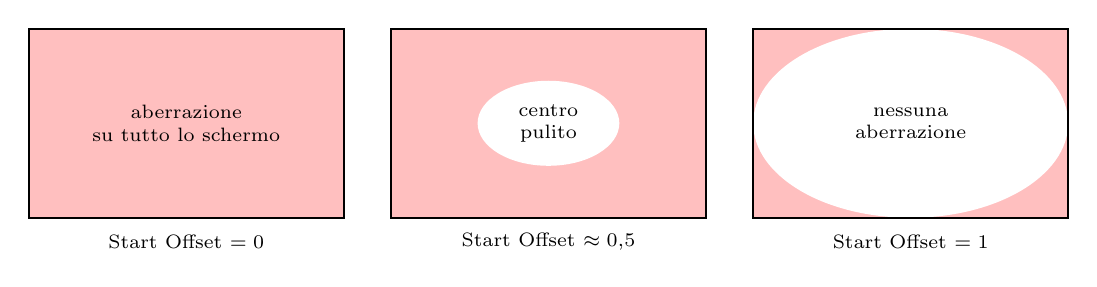
\begin{tikzpicture}[font=\scriptsize, x=1cm, y=1cm]
  \foreach \xs/\r/\lab in {0/0.0/{Start Offset $=0$}, 4.6/0.9/{Start Offset $\approx 0{,}5$}, 9.2/2.0/{Start Offset $=1$}} {
    \begin{scope}[xshift=\xs cm]
      \begin{scope}
        \clip (0,0) rectangle (4,2.4);
        \fill[red!25] (0,0) rectangle (4,2.4);
        \fill[white] (2,1.2) ellipse ({\r} and {\r*0.6});
      \end{scope}
      \draw[thick] (0,0) rectangle (4,2.4);
      \node at (2,-0.3) {\lab};
    \end{scope}
  }
  \node[align=center] at (2,1.2) {aberrazione\\su tutto lo schermo};
  \node[align=center] at (6.6,1.2) {centro\\pulito};
  \node[align=center] at (11.2,1.2) {nessuna\\aberrazione};
\end{tikzpicture}
\caption{Lo Start Offset della Chromatic Aberration: dal centro dello schermo fino al valore
impostato l'immagine resta pulita, oltre compare la separazione dei canali. A 1 l'effetto
sparisce. Ricostruzione schematica.}
\label{ue16:fig:chromatic}
\end{figure}

\paragraph{Approfondimento: aberrazione e accessibilità.} L'aberrazione cromatica imita un
difetto degli obiettivi reali, che non fanno convergere nello stesso punto le diverse
lunghezze d'onda: per questo è più forte ai bordi. Il consiglio del docente coincide con una
pratica diffusa dell'accessibilità: effetti come aberrazione, motion blur, vignettatura forte e
\emph{film grain} affaticano la vista o danno nausea a una parte dei giocatori, e molti giochi
offrono un'opzione per disattivarli. In Unreal si può farlo modificando a runtime le proprietà
del post process (per esempio il \emph{Post Process Settings} di una camera o di un volume da
Blueprint) oppure, per un picco di breve durata come la flashbang, animando l'intensità con una
\emph{Timeline}, lo strumento visto nelle prime lezioni del corso (funzionamento generale
dell'engine). Totten, nel capitolo 5, ricorda che l'horror lavora sull'incertezza percettiva
(l'ombra, la nebbia): l'aberrazione dell'esempio lovecraftiano è la versione
``sullo schermo'' della stessa strategia.

% ---------------------------------------------------------------------
\section{Il Lens Flare}
\label{ue16:sec:flare}

\paragraph{Che cos'è.} ``Questa è un'altra molto comune, molto vista'': ``forse è il tipo di
post-process con cui siamo più familiari'', perché si vede spesso anche nelle immagini delle
fotocamere. È la ``scomposizione dello spettro della luce'': dentro il volume la luce viene
scomposta, e si vedono ``gli esagoni che si creano''. Si può usare ``per diecimila motivi'':
per esempio quando il personaggio è appena uscito all'aperto dopo essere stato al chiuso, e la
scomposizione ``ci accoglie e ci dà un'idea di quanto effettivamente il sole sia forte'', o una
luce in generale.

\paragraph{I parametri.}
\begin{itemize}
  \item \textbf{Intensity}: quanto è forte. ``Se non ricordo male'' è influenzato anche dal
        \textbf{bloom}: ed ``esatto'', aumentando l'intensità del bloom il lens flare diventa
        più sfumato.
  \item \textbf{Tint}: il colore del flare, ``magari prendiamo questo flare violaceo''; si
        può anche modificare a mano il riferimento dei canali RGB.
  \item \textbf{Bokeh Size} (``poke size'': ``sono ignorante su come si pronuncia''): la
        grandezza di ``non lo so neanche come chiamarli, dei cristalli, degli esagoni della
        scomposizione della luce'', per un effetto più o meno scomposto (il docente toglie il
        blu per farlo vedere meglio).
  \item \textbf{Threshold}: ``funziona sempre nello stesso modo'', la soglia minima di
        luminosità per avere l'effetto.
  \item \textbf{Bokeh Shape}: ``devo essere onesto, non ho mai trovato un'utilità a questa
        cosa'', ma si può cambiare la forma dei cristalli con una \textbf{texture}. Quella di
        default si chiama, nella trascrizione, ``Presize default all''; cambiandola si hanno
        cerchi, pentagoni, ``qualsiasi texture abbiamo'': l'icona di un bersaglio, ``un'immaginina
        con delle stelline''. Le texture troppo dettagliate non rendono (``non si nota
        effettivamente il dettaglio''), ma per una questione di forma funzionano; la texture
        porta con sé anche il colore.
  \item \textbf{Tints}: per personalizzare ``al 100\%'' il flare, si può modificare ``ogni
        singolo cristallino'': ce n'è uno viola, uno blu, uno verde, e si decide quali colori
        dello spettro ``risultano maggiormente''. Sono numerati da 0 a 7 (la trascrizione elenca
        ``0, 1, 2, 3, 4, 5, 7'').
\end{itemize}
``Il lens flare lo teniamo, che insomma è piacevole averlo.''

\paragraph{Approfondimento: un difetto che diventa linguaggio.} Il lens flare è un riflesso
interno fra le lenti di un obiettivo, e i suoi esagoni hanno la forma del diaframma; in
Unreal Engine~5 il lens flare del post process è un effetto \emph{image-based}, calcolato a
partire dalle zone più brillanti dell'immagine (per questo dipende dal bloom e dalla soglia),
e la \emph{Bokeh Shape} è appunto la sagoma del diaframma simulato. Nel cinema e nei giochi il
flare comunica ``guardi verso una luce forte'' e, spesso, ``stai guardando attraverso una
camera'': usato ovunque, indebolisce l'idea di una visione in prima persona; usato al momento
giusto, come l'uscita all'aperto del docente, è un segnale di passaggio. Funzionamento generale
dell'engine.

% ---------------------------------------------------------------------
\section{La Depth of Field}
\label{ue16:sec:dof}

\paragraph{Mettere a fuoco.} ``Un'altra cosa molto importante che possiamo utilizzare nel
momento in cui andiamo a fare un render di un'immagine, ma anche quando dobbiamo gestire le
distanze'', è la \textbf{Depth of Field} (la profondità di campo). Permette ``una serie di
modifiche di messa a fuoco'': si modifica la \textbf{distanza focale}, cioè a quale distanza si
mette a fuoco. Nella prova c'è ``una leggera sfocatura'', e più in là ``qualcosa di meno messo a
fuoco, ma comunque non visibilissimo'': ``mettiamo che il nostro personaggio sia vagamente
miope, insomma, vedrà in questo modo qui''.

\paragraph{Gli altri parametri.} Il docente ricorda altri parametri che permettono di
determinare ``la distanza a cui vediamo il blur e l'intensità del blur'': ``quale sia la forza
della sfocatura e da quale distanza venga effettivamente attivata''. Ma ``ricordo funzionasse
in maniera diversa'': ``credo che sulla 4 funzioni in maniera diversa''. Promette di
controllare durante la pausa e di riferire le eventuali modifiche; dopo la pausa, però, la
trascrizione non riporta più nulla sulla depth of field.

\paragraph{Approfondimento: la profondità di campo in Unreal Engine~5.} La differenza che il
docente ricorda c'è davvero. In Unreal Engine~4 esistevano più metodi (\emph{Gaussian},
\emph{Bokeh}, \emph{Circle}), ciascuno con parametri propri come le regioni di transizione
vicina e lontana; in Unreal Engine~5 su PC e console resta di fatto un solo metodo, il
\emph{Cinematic} DOF, i cui parametri principali sono la \emph{Focal Distance} (la distanza
di messa a fuoco, in centimetri), l'\emph{Aperture} o \emph{f-stop} della camera (più è basso,
più la profondità di campo è stretta) e la dimensione del sensore; sono presenti anche
\emph{Depth Blur km for 50\%} e \emph{Depth Blur Radius}, che aggiungono una sfocatura di
distanza indipendente dalla messa a fuoco. Il \emph{Mobile Depth of Field} che il docente vede
nella lista della Camera Actor è la versione semplificata per dispositivi mobili, con distanze
di transizione esplicite, ed è probabilmente il modello di funzionamento che ricordava. Sulla
Camera Actor (\emph{Cine Camera Actor}) la messa a fuoco si regola dalle \emph{Focus Settings},
anche in modo automatico seguendo un actor (funzionamento generale dell'engine). In un gioco
la profondità di campo è utile soprattutto per i menu, i dialoghi e le schermate, dove guida lo
sguardo verso il soggetto: è la stessa funzione che Totten, nel capitolo 7, attribuisce alla
cinematografia, ``attirare l'attenzione del giocatore'' sugli elementi che il designer vuole
fargli vedere.

% ---------------------------------------------------------------------
\section{Il Color Grading}
\label{ue16:sec:grading}

\paragraph{La cosa più famosa.} ``Forse la cosa più famosa per cui è conosciuta e utilizzata
la post-produzione'' è la \textbf{color correction}: applicare all'immagine ``un nuovo stile, un
nuovo tipo di colore'' con una serie di parametri. Il docente richiude tutte le sezioni per
vederle una per una.

\paragraph{Temperature.} ``Di base, il color grading parte dalla \textbf{temperatura}'': una
scena più calda o più fredda, da un estremo all'altro, con ``questa renderizzazione più
giallastra'' o ``completamente sbiancata e bluastra''. Poi la \textbf{tinta} (\emph{Tint}), per
spingere la scena verso il magenta o verso il verde.

\paragraph{Global, Shadows, Midtones, Highlights.} Oltre alla temperatura ci sono i parametri
``che ci permettono di fare una customizzazione più completa'': \textbf{Global},
\textbf{Shadows}, \textbf{Midtones} (``mittons'') e \textbf{Highlights}. Sono la possibilità
di fare color correction su tutta la scena (Global), solo sugli scuri, ``nelle parti più buie,
nelle ombre'' (Shadows), ``nei grigi, nei medi'' (Midtones) e ``nelle luci, nelle parti più
illuminate'' (Highlights) (figura~\ref{ue16:fig:grading}).

\paragraph{Cinque sottoparametri.} ``Funzionano tutti allo stesso modo'': ognuno ha la stessa
lista di \textbf{Saturation}, \textbf{Contrast}, \textbf{Gamma}, \textbf{Gain} e
\textbf{Offset}, da attivare con la spunta ed espandere con la freccia. Con la saturazione si
decide quanto la scena sia satura o desaturata, con lo slider sotto. (A questo punto la
trascrizione si perde per diverse righe in un blocco ripetuto senza senso; quando riprende, il
docente sta parlando del \textbf{contrasto}.) Con il contrasto si gioca sulla differenza ``fra
le luci e le ombre'': la si può accentuare o appiattire, ``una sorta di maschera di contrasto
del colore''. ``Stessa cosa gamma e gain'': moltiplicano la color correction della scena, e si
alzano o abbassano per modificare il colore.

\begin{figure}[htbp]
\centering
\begin{tikzpicture}[font=\scriptsize, x=1cm, y=1cm]
  \shade[left color=black, right color=white] (0,0) rectangle (12,0.7);
  \draw[thick] (0,0) rectangle (12,0.7);
  \draw[thick] (0,1.0) -- (4,1.0);
  \node at (2,1.3) {\textbf{Shadows}: ombre};
  \node at (6,1.3) {\textbf{Midtones}: grigi, medi};
  \node at (10,1.3) {\textbf{Highlights}: luci};
  \draw[thick] (4,0) -- (4,1.1); \draw[thick] (8,0) -- (8,1.1);
  \draw[thick, {Stealth[length=1.6mm]}-{Stealth[length=1.6mm]}] (0,1.8) -- (12,1.8) node[midway, above] {\textbf{Global}: tutta la scena};
  \node[align=center, draw, rounded corners=2pt, fill=gray!10, inner sep=4pt] at (6,-0.9)
    {in ognuna: Saturation $\cdot$ Contrast $\cdot$ Gamma $\cdot$ Gain $\cdot$ Offset};
  \node[align=center, draw, rounded corners=2pt, fill=orange!10, inner sep=4pt] at (6,-1.8)
    {prima, per tutta l'immagine: Temperature (caldo / freddo) e Tint (magenta / verde)};
\end{tikzpicture}
\caption{Le zone del Color Grading. Global agisce su tutta l'immagine, Shadows, Midtones e
Highlights sulle zone scure, medie e chiare; ciascuna ha gli stessi cinque sottoparametri.
I confini fra le zone sono sfumati e regolabili. Ricostruzione schematica.}
\label{ue16:fig:grading}
\end{figure}

\paragraph{Uno strumento avanzato.} ``Il post-process è un elemento molto molto avanzato'':
non perché sia difficile da usare, ``ma nel senso che è difficile ottenere esattamente il
risultato che volete''. È un oggetto con cui ``dovete sperimentare, mettervi là, fare
esperienza'' di come funziona e di quali possibilità ha. ``Se dovessimo esplorarlo al 100\%
ci vorrebbe molto di più di una lezione, e probabilmente non sarei neanche la persona adatta.''
Il docente ha mostrato le lenti ``che potreste utilizzare di più'' per creare un certo
\emph{mood} e un certo tipo di scena; si ferma qui per parlare di altre cose ``ugualmente
importanti'', ``più basilari forse, meno avanzate''. Chi vuole può partire da questa base:
mettere in scena il proprio post process e ``smontarlo un pochino''.

\paragraph{Prima le luci, poi il post process.} La post produzione ``influisce grandemente
sulla luce'': a seconda del tipo di luce in scena si avranno effetti diversi. L'ordine giusto:
prima si costruisce l'illuminazione, ``come abbiamo visto con i light actor qualche lezione
fa'', e solo quando le luci sono posizionate si fa questo lavoro. ``Capisco che è stato molto
brutale e molto rapido'', ma ``più che mostrarvi gli elementi di base e incitarvi a provare a
sperimentare'' non c'è tempo. ``Oggi purtroppo corriamo un po'.''

\paragraph{Approfondimento: colore e significato.} Il color grading di Unreal segue il
modello dei programmi di correzione colore del cinema: Saturation, Contrast, Gamma, Gain e
Offset sono i classici controlli di \emph{lift-gamma-gain} applicati per zone, e i confini
fra Shadows, Midtones e Highlights si regolano con \emph{Shadows Max} e \emph{Highlights Min};
per un controllo totale si può usare una \emph{Color Grading LUT}, una tabella di colori
preparata in un programma esterno (funzionamento generale dell'engine). Totten, nel capitolo 4
(``Basic Color Theory''), fornisce il vocabolario per scegliere: i colori \emph{analoghi}
(tre colori vicini sulla ruota, come blu, blu-viola e viola) creano un'atmosfera armonica e,
in quel caso, ``un senso cupo o freddo''; rosso, rosso-arancio e arancio danno una sensazione
calda; i \emph{complementari} (opposti sulla ruota) creano contrasto. È esattamente il
``posto lugubre'' del docente, caricato di verdi, blu e viola. L'esempio di Totten è
\emph{Bioshock Infinite}: una cappella dominata dal blu in cui le uscite sulla strada
principale sono segnate da elementi complementari, una luce arancione o un fedele in tunica
bianca, mentre i passaggi secondari restano in tinte analoghe. Il color grading regola il
colore dominante; il contrasto che guida il giocatore va poi costruito con le luci e gli
oggetti.

% ---------------------------------------------------------------------
\section{La domanda sull'effetto in due toni}
\label{ue16:sec:duetoni}

\paragraph{La domanda.} Prima di passare al packaging arriva una domanda in chat: ``si possono
applicare effetti di luce più estremi, magari su altri programmi?'' Per esempio ``rendere il
livello in due toni'', ``solo rosso e nero'', per ottenere ``un effetto tipo
\textbf{Limbo}''. ``Sì, si può fare, ma anche già soltanto all'interno di Unreal, utilizzando
un post process volume.''

\paragraph{La zanzara e il cannone.} Il docente sposta però la questione: non è tanto ``se
Unreal lo può fare oppure no'', ma ``per fare quella cosa, è davvero necessario utilizzare
Unreal?'' Se l'idea è creare qualcosa di esteticamente molto semplice, in bianco e nero, si
può forse realizzarlo con altri engine. ``Teniamo sempre a mente che Unreal è un engine pesante
che fa le cose in maniera pesante.'' Se si vuole rifare Limbo, ``che magari è anche in 2D'' e
quindi più semplice, e lo si fa in Unreal, ``stiamo sparando a una zanzara con un cannone'':
``la zanzara l'ammazziamo, però smontiamo pure quello che c'è dietro''. Quanto agli ``altri
programmi'': se si fa un'immagine in Unreal, uno screenshot di un ambiente, e la si modifica
``in post'' con un programma di fotoritocco, ``sì, lo posso fare''.

\paragraph{Mallory.} Lo studente cita un gioco, ``Mallory'' (``Mellori'' più avanti; il nome
esatto non è ricostruibile dalla trascrizione), un titolo per Switch fatto in Unreal, e
condivide dei link. Il docente non lo conosce: ``poi me lo guardo durante la pausa''. In ogni
caso, ``se è fatto in Unreal si può fare tranquillamente'': l'idea stessa del Post Process
Volume è avere un oggetto in scena che permette di passare da un tipo di post produzione a un
altro o di controllarla meglio; ``una volta che mi impratichisco con lo strumento posso fare
un po' quello che mi pare''. Serve però anche gestire bene l'illuminazione: ci si costruisce
l'illuminazione ``come è gestita in quel titolo'' e poi la si modifica a posteriori. (Il
seguito, dopo la pausa, è nella sezione~\ref{ue16:sec:pausa}.)

\paragraph{Approfondimento: scegliere l'engine.} La metafora del cannone tocca un tema di
produzione: il costo di un engine non è solo la licenza, ma il peso dei progetti, i tempi di
compilazione degli shader e del packaging (che il docente sperimenterà di lì a poco) e le
macchine richieste ai giocatori, come ha scoperto lo studente con il portatile che ``non
reggeva''. Per un gioco 2D stilizzato un engine più leggero è spesso la scelta più efficiente;
Unreal ha comunque strumenti 2D (\emph{Paper2D}, gli sprite e i flipbook citati nella lezione
precedente). Un effetto ``in due toni'' in Unreal si ottiene con un \emph{Post Process
Material}: un materiale con dominio \emph{Post Process}, assegnato nei \emph{Rendering
Features} del volume (\emph{Post Process Materials}), che legge il colore della scena e lo
riduce a due colori secondo una soglia di luminosità (funzionamento generale dell'engine).
Totten, nel capitolo 4, usa proprio \emph{Limbo} come esempio di linguaggio visivo: il gioco
gioca il suo stile a silhouette contro le convenzioni del giocatore, come nel puzzle della
pressa in cui il ``pulsante'' rialzato non è il vero meccanismo. Lo stile in due toni, lì, non
è un filtro sopra il gioco: è parte delle regole con cui il giocatore legge lo spazio.

% ---------------------------------------------------------------------
\section{Il packaging: che cos'è e dove si avvia}
\label{ue16:sec:packaging}

\paragraph{Che cos'è.} ``Il packaging è un processo che viene fatto principalmente da Unreal
Engine, in realtà, per cui noi dobbiamo andare a curare soltanto alcune impostazioni.'' È ciò
che ``ci consente di andare a creare un \textbf{eseguibile} con quello che noi abbiamo
all'interno dell'editor''.

\paragraph{Platforms.} Il packaging si avvia dal pulsante \textbf{Platforms} della barra degli
strumenti. Scendendo si vedono ``tutte le varie piattaforme per cui potremmo sviluppare
qualcosa'': \textbf{Android}, \textbf{iOS}, \textbf{Linux}, \textbf{Mac}, \textbf{Windows}.
Accanto ad alcune c'è ``sempre questo segnale di attenzione'': il docente è su Windows, e il
progetto ``non è gestito o pensato'' per funzionare anche sugli altri sistemi. Nella voce
\textbf{Windows} ci sono il \textbf{Package Project}, ``il pulsantone che io premo se voglio far
partire questo processo'', e la scelta della \textbf{configurazione}. ``Queste sono pochissime
impostazioni, e non sono neanche lontanamente tutte quelle che ci servono'': le altre sono nei
\textbf{Project Settings}, la ``macro sezione di setting e di impostazioni per tutto il nostro
progetto'' già vista con Igor (figura~\ref{ue16:fig:packaging}).

\paragraph{Il plugin di Fab.} Un'altra finestra che può servire è quella dei \textbf{Plugins},
che permette di attivare e disattivare i plugin. ``Da quello che so, il plugin di
\textbf{Fab} dà dei problemi con il packaging'': quindi, prima di impacchettare, lo si
disattiva. ``Non so se è stato risolto. Potrebbe essere stato risolto, dovrei informarmi.''

% ---------------------------------------------------------------------
\section{Le impostazioni del progetto}
\label{ue16:sec:impostazioni}

\paragraph{Maps \& Modes.} Nei Project Settings, nella pagina \textbf{Maps \& Modes}, ``oltre
alla Game Mode'', ci sono le \textbf{Default Maps}: \textbf{Editor Startup Map} e
\textbf{Game Default Map}.
\begin{itemize}
  \item L'\textbf{Editor Startup Map} è la mappa con cui si apre l'editor: se la si cambia,
        ``ogni volta che io aprirò questo progetto lui mi partirà da quell'altra mappa'', e per
        tornare al livello di prima bisognerà riaprire a mano la Third Person Map.
  \item La \textbf{Game Default Map} è ``allo stesso modo la mappa di partenza che avremo
        all'interno del nostro eseguibile''. Se il gioco ha un menu che porta alla mappa di
        gioco, non si mette la Third Person Map: ``di solito quello che si fa è mettere un
        \textbf{menu principale}'', o una schermata che, dopo aver cliccato qualche pulsante,
        porta alle mappe che si vogliono giocare.
\end{itemize}
Sono due impostazioni importanti: ``se mai vi capiterà di dire: oddio, dove è andata la mia
mappa, perché si è aperto così, dove sono finito, cosa è successo''; oppure ``per quale motivo
ho fatto il packaging e non mi fa partire da dove dico io'': è la Game Default Map da
modificare. (Il docente scorre altre voci della pagina, ``ma questa non è necessaria'', senza
nominarle.)

\paragraph{Supported Platforms.} Un'altra pagina è quella delle \textbf{Supported Platforms}.
Di default è impostata su \textbf{All Platforms}; togliendo la spunta e lasciando solo ciò che
interessa si può avere, per esempio, soltanto \textbf{Windows} come piattaforma per il
packaging, ``perché il nostro progetto magari non supporta tutti gli altri sistemi
operativi''.

\paragraph{La pagina Packaging.} ``Ultima cosa, ma la più importante'': c'è una pagina tutta
dedicata al \textbf{packaging}. ``Sono un sacco di informazioni, un sacco di parametri'', ma
``la cosa positiva è che la maggior parte di questi parametri sta bene come sta'': non servono
``modifiche assurde''. Alcune voci si vedono subito, altre solo aprendo gli
\textbf{Advanced}. Le prime: \textbf{Build}, ``va bene così'' (l'opzione ``if project has code
or running a locally built editor'', che lascia decidere all'engine se compilare); poi la
\textbf{Build Configuration}.

% ---------------------------------------------------------------------
\section{Le configurazioni di build}
\label{ue16:sec:build}

\paragraph{Cinque configurazioni, tre disponibili.} La \textbf{Build Configuration} decide
``che tipo di configurazione avrà il nostro eseguibile'': \textbf{Debug}, \textbf{DebugGame},
\textbf{Development}, \textbf{Test} e \textbf{Shipping}. ``Per la build che abbiamo scelto''
ne sono attive soltanto tre (le stesse che si ritrovano poi nel menu Platforms: DebugGame,
Development e Shipping). Le differenze (tabella~\ref{ue16:tab:build}):
\begin{itemize}
  \item \textbf{Debug} e \textbf{DebugGame} ``sono modalità di debug'': un eseguibile in cui
        c'è ancora una \textbf{console di comandi} per inserire comandi, fare aggiustamenti,
        ``vedere le linee, vedere quello che sta succedendo, vedere dei text che vengono
        printati''. ``È una versione super di test.''
  \item \textbf{Development} è ``la configurazione di default di Unreal''. Rimuove la maggior
        parte della struttura di debug, aumenta un po' l'ottimizzazione della build, ``ma
        mantiene comunque alcuni strumenti che possono essere utilizzati per il testing''. ``Se
        debug è un eseguibile che può essere di uso a un \textbf{programmatore}, development può
        essere di uso a un \textbf{designer}'': si può ancora modificare qualcosa e usare degli
        input, ma serve soprattutto per testare e poi ritoccare in engine.
  \item \textbf{Shipping} è la modalità ``per la distribuzione'': ``il progetto finito, il
        gioco che le masse giocheranno, si spera le masse''. È ``la versione più ottimizzata
        possibile della build'', ``la build da vendita, praticamente''.
\end{itemize}

\paragraph{Shipping non ottimizza da solo.} ``Aspettate: questo non vuol dire che lui vi
ottimizzi le cose in automatico.'' L'ottimizzazione ``è tutto un discorso a parte, che va fatto
separatamente'': far sì che non ci siano troppe linee di codice, che non ci siano texture a
qualità troppo alta o non utilizzate, eccetera. Shipping ``vuol dire semplicemente che lui va a
togliere tutta una serie di strumenti che non servono più''.

\begin{table}[htbp]
\centering
\small
\begin{tabular}{@{}p{2.3cm}p{5.6cm}p{3.0cm}p{3.1cm}@{}}
\toprule
\textbf{Configurazione} & \textbf{Che cosa contiene (lezione)} & \textbf{Per chi} &
\textbf{Nota} \\
\midrule
Debug & console di comandi, linee, testi stampati: ``versione super di test'' &
programmatore & richiede un progetto con codice C++ \\
DebugGame & come sopra, debug del codice di gioco & programmatore & disponibile \\
Development & default di Unreal; meno debug, un po' più ottimizzata, alcuni strumenti di test
& designer, tester & disponibile; console attiva \\
Test & vicina a Shipping, con qualche strumento di profilazione & QA & richiede codice C++ \\
Shipping & la versione finale, senza strumenti di sviluppo & i giocatori & disponibile; non
ottimizza da sola \\
\bottomrule
\end{tabular}
\caption{Le cinque configurazioni di build. Nel progetto del docente ne sono attive tre; la
colonna ``Nota'' integra con il funzionamento generale dell'engine.}
\label{ue16:tab:build}
\end{table}

\paragraph{Le lingue.} Aprendo gli Advanced si trovano le \textbf{lingue} del packaging
(\emph{Localizations to Package}): ``possiamo andare a selezionare che tipo di lingue dovranno
essere utilizzate''. ``Di default c'è solo l'inglese.'' Se si è localizzato qualcosa, per
esempio perché ci sono già impostazioni e parametri che fanno riferimento a certe lingue, qui
si scelgono quelle da includere.

\paragraph{Approfondimento: le configurazioni secondo Romero e Sewell.} Romero e Sewell, nel
capitolo 12 (``Building and Publishing''), descrivono lo stesso percorso: \emph{Platforms}
$\rightarrow$ piattaforma $\rightarrow$ \emph{Package Project}, la scelta della cartella, la
finestra che avvisa che l'engine sta impacchettando e, in caso di problemi, ``i dettagli
dell'errore nella finestra dell'output log''. Prima, nei \emph{Project Settings}: la pagina
\emph{Description} (nome, miniatura, descrizione del progetto), la pagina \emph{Maps \& Modes}
(``spesso dovrete designare una mappa dedicata al menu principale come prima mappa da
caricare'', e assicurarsi che sia lei a gestire quale mappa si carica dopo) e la pagina della
piattaforma, dove per Windows si cambiano lo \emph{splash screen} e l'\emph{icona}
dell'eseguibile. Sulle configurazioni il libro precisa che nei progetti \emph{solo
Blueprint} le opzioni principali sono \textbf{Development}, che contiene informazioni di debug
utili a trovare errori, e \textbf{Shipping}, ``più pulita'', da usare per la versione da
distribuire; Debug e Test richiedono un progetto con codice C++ (ed è per questo che nel
progetto del docente sono spente). Il libro nomina anche la \emph{Staging Directory}, la
cartella in cui viene salvata la build, l'opzione \emph{For Distribution}, richiesta per
pubblicare su App Store o Google Play, e lo \emph{Zip Project} del menu File, che comprime i
file essenziali del progetto per passarlo a un'altra persona. Una nota importante dello stesso
capitolo: Unreal Engine~5 può creare build Windows solo da Windows e build macOS solo da macOS;
è il ``segnale di attenzione'' che il docente vede accanto alle altre piattaforme.

% ---------------------------------------------------------------------
\section{Le mappe e le cartelle da cucinare}
\label{ue16:sec:cook}

\paragraph{Cook only maps.} ``Fare il packaging di base vuol dire che lui prende tutto il
progetto e lo rende pronto per essere un eseguibile'', con un certo metodo di compressione.
Spuntando \textbf{Cook only maps} (``hook only maps'' nella trascrizione), invece, il
packaging usa ``unicamente le mappe'': si può dirgli di usare soltanto la Third Person Map, e
lui ``si vede cosa c'è dentro'', mette nel pacchetto ``tutto quello che serve per far funzionare''
quella mappa ``e non mette il resto delle cose''.

\paragraph{List of maps to include.} Insieme a Cook only maps serve la voce \textbf{List of maps
to include in a packaged build}. Si aggiunge un elemento, si clicca sui tre puntini e si cerca
la mappa: ``volete level 1, level 2, menu? Magari vi serve il menu''. Nel caso della prova
serve soltanto la Third Person Map (il file \texttt{.umap}): ``non serve andare a inserire anche
il build data'' (il file \texttt{\_BuiltData}) ``o lo \texttt{.uasset}''. Si possono aggiungere
altre mappe, copiarle, eliminarle.

\paragraph{Directories to never cook.} ``Un'altra cosa che ci torna utile'' è
\textbf{Directories to never cook}: le cartelle che non devono mai finire nel pacchetto. Si
aggiunge un elemento (``un index zero'') e si sceglie la cartella. Gli esempi:
\begin{itemize}
  \item ``nulla di \emph{GameApps}'' (il nome della cartella, nella trascrizione, è ``game
        apps'') ``deve finire dentro il packaging'';
  \item una cartella con ``tutta una serie di modelli 3D molto fighi'' che non si è riusciti a
        inserire e che magari si vogliono usare in un \textbf{DLC} più avanti.
\end{itemize}
I motivi sono due. Il primo è il \textbf{data mining}, ``diventato super popolare adesso'': i
file messi nel gioco ``possono essere ritrovati da chi va a scavare''. Il secondo: sono comunque
cose ``che vanno ad essere cucinate e vengono comunque inserite all'interno della build''.
Togliere le cartelle che non servono ``ci fa risparmiare giga'': un progetto più piccolo e più
semplice da gestire (tabella~\ref{ue16:tab:packaging}).

\begin{table}[htbp]
\centering
\small
\begin{tabular}{@{}p{4.6cm}p{2.8cm}p{6.6cm}@{}}
\toprule
\textbf{Impostazione} & \textbf{Dove} & \textbf{A che cosa serve} \\
\midrule
Package Project, configurazione & Platforms $\rightarrow$ Windows & avviare il packaging;
scegliere DebugGame, Development, Shipping o le impostazioni del progetto \\
Plugin di Fab & Edit $\rightarrow$ Plugins & disattivarlo prima del packaging (problemi
noti, forse risolti) \\
Editor Startup Map & Maps \& Modes & la mappa con cui si apre l'editor \\
Game Default Map & Maps \& Modes & la prima mappa dell'eseguibile: di solito il menu \\
Supported Platforms & Project Settings & limitare le piattaforme (per esempio solo Windows) \\
Build & Packaging & lasciare il default \\
Build Configuration & Packaging & Debug, DebugGame, Development, Test, Shipping \\
Localizations to Package & Packaging (Advanced) & le lingue incluse; default inglese \\
Cook only maps & Packaging (Advanced) & impacchettare solo ciò che serve alle mappe elencate \\
List of maps to include & Packaging (Advanced) & le mappe (\texttt{.umap}) da includere \\
Directories to never cook & Packaging (Advanced) & cartelle escluse: asset scartati, DLC,
spazio \\
Show Output Log & finestra del packaging & seguire il processo e trovare gli errori in rosso \\
\bottomrule
\end{tabular}
\caption{Le impostazioni del packaging viste a lezione, nell'ordine in cui il docente le
mostra.}
\label{ue16:tab:packaging}
\end{table}

\paragraph{Approfondimento: che cosa vuol dire ``cucinare''.} Il \emph{cooking} è la fase in
cui l'engine converte gli asset dal formato dell'editor a quello ottimizzato per la
piattaforma di destinazione: compila gli shader, comprime le texture, elimina i dati che
servono solo all'editor. Il packaging vero e proprio raccoglie poi gli asset cucinati in
archivi (\emph{.pak}, o \emph{IoStore} in Unreal Engine~5) accanto all'eseguibile. Con Cook
only maps disattivato l'engine cucina di norma tutto il contenuto del progetto, compresi gli
asset mai usati; con l'opzione attiva segue le \emph{reference} a partire dalle mappe
elencate. Un'avvertenza: un asset caricato solo per nome, a runtime (per esempio con un
percorso scritto in una stringa), non è una reference visibile al cook e rischia di restare
fuori; per questi casi esistono le voci \emph{Additional Asset Directories to Cook}. Anche
\emph{Directories to never cook} va usata con attenzione: se un asset escluso è referenziato
da una mappa inclusa, il cook segnala un errore o il gioco lo perde (funzionamento generale
dell'engine). Totten, nel capitolo 2, parla di \emph{modular design} e di ``schedule'' dei
pezzi di un livello: sapere fin dalla pre-produzione quali pezzi servono rende più facile
anche sapere, alla fine, che cosa lasciare fuori.

% ---------------------------------------------------------------------
\section{L'avvio del packaging e l'Output Log}
\label{ue16:sec:avvio}

\paragraph{Dove salvare.} Per avviare si torna al menu Platforms: lì si vedono le
configurazioni (``debug'', \textbf{Development} e \textbf{Shipping}, ``perché sono le tre
possibili''), oppure \emph{Use Project Setting}, cioè quelle della pagina Packaging. Il docente
sceglie \textbf{Development}. Con \textbf{Package Project} si apre una finestra che chiede dove
creare il pacchetto; il docente sceglie il desktop, e parte il processo, accompagnato da un
``suonino''.

\paragraph{La prima volta è lenta.} ``Fare un packaging la prima volta è molto lento'', anche
se è solo di una mappa. ``Dopo il primo packaging diventa tutto molto più veloce.'' Mentre
lavora (``parte \emph{Cancel}, chiaramente'', per interromperlo) si può aprire lo
\textbf{Show Output Log}: lì si vede tutto quello che sta succedendo. Scorrendolo (``con la
rotella del mio mouse che è rotta è tremendo'') si controlla se va tutto bene, se ci sono
errori o ``piccoli problemi'', o cose che creano problemi al packaging. In quel momento
l'engine sta facendo ``la compilazione degli shader''.

\paragraph{La scritta rossa.} ``Arriverà un punto in cui magari c'è una scritta rossa.'' La
scritta rossa ``vuol dire che c'è un problema che gli impedisce di fare il packaging''. Si legge
che cosa dice, si risolve quel problema, e si riprova.

\paragraph{Che cosa esce.} Se il processo finisce, nella cartella scelta si crea una cartella
che, ``se non gli viene dato un nome'', si chiama \textbf{Windows No Editor} (in Unreal
Engine~5 è semplicemente \emph{Windows}; \emph{WindowsNoEditor} era il nome di Unreal
Engine~4). Dentro c'è l'\textbf{eseguibile}: avviandolo parte il progetto, che in questo caso
sarebbe soltanto la Third Person Map, ``perché è l'unica mappa che gli abbiamo detto di
cucinare''. Il personaggio spawna sul \textbf{Player Start} e può andare in giro: ``non c'è un
obiettivo, non c'è una fine, non c'è nulla''.

\paragraph{I confini della mappa.} ``Chiaramente, per un packaging, non dovrebbero esserci
posti in cui puoi buttarti di sotto nel nulla, come il bordo della mappa''; né posti ``in cui
io non voglio che i giocatori vadano''. Nessuna domanda sul packaging. Siccome ci vorrà ``un
po' troppo tempo'', il docente anticipa la pausa, ``in modo che forse durante la pausa lui
finisca di calcolare'' e si possa vedere che cosa genera. Dopo la pausa: ``un paio di altri
attori'' utili quando si fa un livello, il Blueprint delle \textbf{spline}, ``che potete
utilizzare per un sacco di elementi diversi'', e, ``se ci avanza un po' di tempo'', le
\textbf{decal}, ``un altro strumento di decoro, di arredo'' per aggiungere dettagli in giro per
la mappa. ``Facciamo un 15 minuti di stop. Ci rivediamo alle 5 e mezza.''

\begin{figure}[htbp]
\centering
\begin{tikzpicture}[font=\scriptsize, x=1cm, y=1cm,
  ue16step/.style={draw, thick, rounded corners=2pt, fill=white, align=center, text width=2.6cm, minimum height=1.1cm, inner sep=3pt},
  ue16arr/.style={-{Stealth[length=1.8mm]}, thick}]
  \node[ue16step, fill=gray!10] (a) at (0,0) {Plugins:\\disattivare Fab};
  \node[ue16step, fill=blue!8] (b) at (3.3,0) {Maps \& Modes:\\Game Default Map\\(il menu)};
  \node[ue16step, fill=blue!8] (c) at (6.6,0) {Packaging:\\configurazione,\\lingue, mappe,\\cartelle escluse};
  \node[ue16step, fill=orange!12] (d) at (9.9,0) {Platforms $\rightarrow$\\Windows $\rightarrow$\\Package Project};
  \node[ue16step, fill=red!8] (e) at (9.9,-2.2) {Output Log:\\shader, cook;\\scritte rosse?};
  \node[ue16step, fill=green!12] (f) at (6.6,-2.2) {cartella \emph{Windows}\\con l'eseguibile};
  \node[ue16step, fill=green!12] (g) at (3.3,-2.2) {ritestare il gioco\\impacchettato};
  \node[ue16step, fill=green!12] (h) at (0,-2.2) {caricare (itch.io,\\Drive) e link\\su Discord};
  \draw[ue16arr] (a) -- (b); \draw[ue16arr] (b) -- (c); \draw[ue16arr] (c) -- (d);
  \draw[ue16arr] (d) -- (e); \draw[ue16arr] (e) -- (f); \draw[ue16arr] (f) -- (g);
  \draw[ue16arr] (g) -- (h);
  \draw[ue16arr, red!70!black] (e.east) -- ++(0.6,0) |- node[pos=0.25, right, align=left] {errore:\\risolvere\\e ripartire} (d.east);
\end{tikzpicture}
\caption{Il percorso del packaging come emerge dalla lezione, fino al consiglio finale di
ritestare il gioco impacchettato e condividerlo. Ricostruzione schematica.}
\label{ue16:fig:packaging}
\end{figure}

% ---------------------------------------------------------------------
\section{La pausa e Mallory}
\label{ue16:sec:pausa}

\paragraph{Il packaging non finisce.} Durante la pausa la trascrizione contiene soltanto il
blocco ripetuto già visto, che non appartiene alla lezione. Alla ripresa: ``purtroppo noi ci
siamo, ma Unreal ancora no, ancora non ho finito col packaging''. Il docente lo interrompe,
``perché sennò mi impedisce di fare altre robe'': ``non pensavo ci volesse così tanto tempo''.
Il risultato del packaging, quindi, non viene mostrato.

\paragraph{Mallory, visto.} Il docente ha guardato il gioco segnalato prima. ``Sembra molto
carino'': non l'ha potuto giocare, ma dal video ``sembra un platform simpatico con un bell'ambiente''.
Non gli è sembrato che ci sia ``un eccessivo utilizzo del post-process''. Quello che fanno
``sicuramente'' è cambiare il modo in cui vengono renderizzate luci e ombre: ``ci sono delle parti
con le ombre che sono molto rossastre rispetto alla luce, che magari è una luce più neutra'',
``una piccola vignettatura'' e ``un effetto di sfocatura messa davanti alla camera''. Lo
studente ha in mente anche altri titoli; il docente osserva che il genere platform ``ora come ora
è messo in mano agli indipendenti'': ``non ci sono più grossi titoloni che fanno quel tipo di
roba''. È giusto cercare ``cose carine fatte da persone in giro'', su Twitch o fra i piccoli
titoli su Steam. ``Purtroppo non è proprio il mio genere'', a parte ``i vecchi classiconi PS1,
PS2''.

\paragraph{Come rifare quell'effetto.} Le indicazioni del docente:
\begin{itemize}
  \item una \textbf{Dirt Mask}, come effetto di camera: una texture sovrapposta alla lente. Fra
        le texture del progetto non ce n'è una adatta; una ``un po' più fitta'' dà già ``questa
        specie di effetto statico, tra virgolette, sulla camera'', da gestire poi con i colori
        corretti (quella provata rende la Dirt Mask rossa: ``se riesci a fartela di effetto
        statico perfetto, potrebbe non essere male'');
  \item negli \textbf{Image Effects}, una piccola \textbf{vignettatura} (\emph{Vignette
        Intensity}), che ``va a scurire lo schermo'' nelle parti esterne e dà ``già di base'' un
        mood un po' più scuro;
  \item il resto ``è tutta \textbf{color correction}'': modificare i colori delle ombre per
        avvicinarli a quelli delle luci, desaturare un po' la scena (``c'è fondamentalmente una
        scala di grigio e in più c'è il rosso, barra rosa'') e mettere ``un accento sul rosso''
        dove c'è il rosso.
\end{itemize}

\paragraph{Monument Valley.} Mallory ricorda al docente, per la struttura dei livelli ``molto
geometrici, molto quadratosi'', i \textbf{Monument Valley}: ``non sono dei platform, sono dei
puzzle game misto opera estetica''. Si basano sull'\textbf{illusione ottica}: il personaggio
``cammina su un corridoio e poi improvvisamente inizia a camminare sulla parete e poi passa
dietro la scena'', e bisogna ruotare il livello per capire dove sta andando. ``Faccio fatica a
descriverli, però cercali, sono molto carini.'' Poi si torna al programma: ``post process,
rapidamente e bruttamente, ma lo abbiamo visto''.

\paragraph{Approfondimento: accentare un colore.} L'``accento sul rosso'' in una scena
desaturata è un'applicazione diretta del contrasto di Totten (capitolo 4): un elemento di un
colore diverso dal dominante attira l'attenzione, e se il colore è sempre lo stesso diventa un
segnale che il giocatore impara a leggere. In Unreal non c'è un controllo per ``desaturare
tutto tranne il rosso'' nel color grading standard: lo si ottiene con un Post Process Material
o, più semplicemente, desaturando con il post process e dando agli oggetti rossi materiali con
un po' di \emph{emissive}, così che restino saturi anche dopo la correzione. La vignettatura si
regola con \emph{Vignette Intensity} negli \emph{Image Effects}; la Dirt Mask nella sezione
\emph{Lens}, con \emph{Dirt Mask Texture}, \emph{Intensity} e \emph{Tint}, ed è visibile solo
dove c'è bloom (funzionamento generale dell'engine). Totten, nel capitolo 4, nota anche come
le associazioni dei colori passino nei giochi: rosso e verde per la salute, blu per la magia.

% ---------------------------------------------------------------------
\section{Le spline: che cosa sono}
\label{ue16:sec:spline}

\paragraph{Una linea.} Il docente ha preparato due Blueprint ``al volo prima di cominciare la
lezione''. Prima, però, ``che cos'è una spline?'' È un \textbf{component} che si può aggiungere
ai Blueprint, ma ``in realtà è proprio un tipo di oggetto'' con una funzione ben specifica, che
si usa anche per modificare il funzionamento del \textbf{landscape} (le \emph{landscape
spline}). Il docente crea un Blueprint di prova con un \textbf{Spline Component}; il tooltip
dice che è ``una spline shape che può essere usata per altri scopi, tipo animare oggetti''.
``È una linea, fondamentalmente.''

\paragraph{Punti e tangenti.} Messa in scena, la spline ``non è nient'altro che una linea'' che
si può allungare, curvare e arricchire di punti (figura~\ref{ue16:fig:spline}):
\begin{itemize}
  \item all'inizio ha \textbf{due punti}, l'inizio e la fine;
  \item cliccando sul punto finale compaiono altri due punti, la \textbf{tangente}; spostandola,
        la spline si curva;
  \item per creare \textbf{nuovi punti} si fa come quando si copia un oggetto: sulla freccia
        del gizmo, \textbf{Alt} premuto, si trascina, ``e ho fatto una copia''; ogni punto
        nuovo curva la linea, si può alzare, spostare, fino a costruire ``una figura, una
        struttura'';
  \item con il tasto destro, \textbf{Delete Spline Point} elimina un punto (la spline si
        riempie da sola fra i punti rimasti, ``lui autofilla'') e \textbf{Add Spline Point
        Here} ne aggiunge uno.
\end{itemize}

\begin{figure}[htbp]
\centering
\begin{tikzpicture}[font=\scriptsize, x=1cm, y=1cm]
  \draw[very thick, blue!70!black] (0,0) .. controls (2,0) and (2.5,2) .. (4.5,2)
                                   .. controls (6.5,2) and (6.5,0) .. (8.5,0.3)
                                   .. controls (10,0.5) and (10.5,1.6) .. (11.5,1.8);
  \foreach \p/\n in {(0,0)/0, (4.5,2)/1, (8.5,0.3)/2, (11.5,1.8)/3} {
    \fill[white, draw=black, thick] \p circle (3pt);
    \node[below=4pt] at \p {punto \n};
  }
  % tangente sul punto 1
  \draw[thick, red!70!black, {Stealth[length=1.5mm]}-{Stealth[length=1.5mm]}] (2.9,2) -- (6.1,2);
  \fill[red!70!black] (2.9,2) circle (2pt); \fill[red!70!black] (6.1,2) circle (2pt);
  \node[above, red!70!black] at (4.5,2.1) {tangente: lunghezza e verso curvano la linea};
  \node[align=left, anchor=west] at (0,-1.1) {Alt + trascinamento su un punto: nuovo punto \quad
    tasto destro: Add Spline Point Here, Delete Spline Point};
  \node[align=left, anchor=west] at (0,-1.6) {segmenti = punti $-$ 1 (qui 4 punti, 3 segmenti: indici da 0 a 2)};
\end{tikzpicture}
\caption{Una spline con quattro punti. Ogni punto ha una posizione e una tangente; i segmenti
sono uno in meno dei punti. Ricostruzione schematica.}
\label{ue16:fig:spline}
\end{figure}

% ---------------------------------------------------------------------
\section{A che cosa servono le spline}
\label{ue16:sec:usi}

\paragraph{Il muro di spine.} ``Immaginate di poter piazzare un oggetto lungo questa linea, o
di poter modellare un oggetto lungo questa linea.'' La storia che il docente racconta gli è
successa ``quando stavo in Accademia'', quando aveva cominciato a ``smanettare con questo
strumentino''. Bisogna creare un \textbf{muro di spine}, come nella \emph{Bella addormentata
nel bosco}, ``tutte le spine attorno al castello''. Due strade:
\begin{itemize}
  \item andare dall'``amico grafico'' e chiedergli ``un muro di spine fatto così, così e così'':
        una mesh ``non particolarmente impegnativa'', ma che richiede tempo e che, se va
        modificata, deve tornare in un software di modellazione come \textbf{Blender} o
        \textbf{Maya};
  \item ``una roba un po' più intelligente'': farsi creare soltanto un \textbf{cilindro di
        spine} e \emph{replicarlo} lungo una spline, così che la mesh ``viene ricreata e viene
        modificata sulla base della spline'', seguendone l'andamento.
\end{itemize}

\paragraph{Altri usi.} ``Al di là di questa cosa'', la struttura serve per molte cose: una
\textbf{pista} per un gioco di macchine (``vi create un blueprint di spline con la strada''); un
\textbf{muro} più stondato nel blockout o nella gym, per esempio ``che sale a spirale verso
l'alto'', quando ``non avete nulla che ve lo fa fare in maniera comoda''. Il docente lo mostra
``in due forme, in due versioni'': una ``più semplice e più brutta'', l'altra ``un po' più
funzionale''. I Blueprint si chiamano \textbf{Spline by Length} e \textbf{Spline by Point}.

\paragraph{La mesh del tubo.} Per la prova usa un tubo, ``un oggetto molto semplice'' che è
anche nel progetto degli studenti: \textbf{SM\_PipeSplineBody} (``Sm pipe spline body''). Il
docente prima dice che ``non è fatto benissimo per essere un oggetto da spline'', poi si
corregge: ``ho detto una cazzata, l'avevo vista in maniera veloce prima''. Funziona bene
perché è \textbf{segmentato}: ha i suoi triangoli e ``questa spezzatura in orizzontale'', è
\textbf{modulare} (``cilindro, cilindro, cilindro''). Questo permette al Blueprint di
replicarlo ``senza andarlo a spezzare'', perché la struttura del tubo viene replicata cilindro
per cilindro. Nella prima versione, allungando la spline il cilindro si allunga; piegandola,
si piega ``però si spezza'', perché è fatta ``in una maniera meno ottimale''; nella seconda ``si
spacca'' ancora, ma ``dovrebbe notarsi di meno''. La differenza (figura~\ref{ue16:fig:pointlength}):
``il primo blueprint, by point, \emph{stretcha} l'oggetto; questo invece ricrea l'oggetto per
lunghezza, quindi è un pochino più fedele''.

\begin{figure}[htbp]
\centering
\begin{tikzpicture}[font=\scriptsize, x=1cm, y=1cm]
  % by point
  \node[anchor=west] at (0,2.9) {\textbf{Spline by Point}: una mesh per ogni segmento, stirata fino al punto successivo};
  \foreach \a/\b/\c in {0/4.2/blue!20, 4.2/6.2/green!20, 6.2/12/orange!20} {
    \draw[thick, fill=\c] (\a,1.6) rectangle (\b,2.4);
  }
  \foreach \x in {0,4.2,6.2,12} \fill[black] (\x,2.0) circle (2.2pt);
  \node at (2.1,2.0) {stirata}; \node at (5.2,2.0) {schiacciata}; \node at (9.1,2.0) {molto stirata};
  % by length
  \node[anchor=west] at (0,1.0) {\textbf{Spline by Length}: una mesh ogni \emph{Mesh Length}, sempre proporzionata};
  \foreach \i in {0,...,5} {
    \draw[thick, fill=blue!20] ({\i*2},-0.2) rectangle ({\i*2+2},0.6);
  }
  \foreach \x in {0,12} \fill[black] (\x,0.2) circle (2.2pt);
  \draw[{Stealth[length=1.4mm]}-{Stealth[length=1.4mm]}] (0,-0.45) -- (2,-0.45) node[midway, below] {Mesh Length (250)};
  \node[align=center] at (9,-0.7) {anche con due soli punti: tanti pezzi quanti\\ne stanno nella lunghezza della spline};
\end{tikzpicture}
\caption{Le due versioni del Blueprint su una spline dritta. Per punto, il numero di mesh è
uno in meno dei punti e ciascuna si deforma fino al punto successivo; per lunghezza, il numero
di mesh dipende dalla lunghezza della spline divisa per quella della mesh. Ricostruzione
schematica.}
\label{ue16:fig:pointlength}
\end{figure}

% ---------------------------------------------------------------------
\section{Il Blueprint per punto}
\label{ue16:sec:bypoint}

\paragraph{La struttura.} Nel \textbf{Spline by Point} la viewport contiene la spline e
``un oggetto che poi gli abbiamo attaccato con un nodo''; l'Event Graph è vuoto, e tutto è nel
\textbf{Construction Script}. ``È una struttura abbastanza semplice'', usabile ``tranquillamente''
per un lavoro di blockout, ``di prototipazione''. Alcune cose il docente le fa ``un po' più
veloce, perché probabilmente le avete già viste anche con Igor''. Il grafo
(figura~\ref{ue16:fig:grafopoint}):
\begin{enumerate}
  \item un \textbf{For Loop}, ``perché dobbiamo loopare un oggetto''. Il \emph{First Index} è
        \textbf{0}, ``la base dell'indice''. Il \emph{Last Index} viene dal numero di punti della
        spline, preso trascinando la spline nel grafo e usando \textbf{Get Number of Spline
        Points}; al numero si \textbf{sottrae 2}. Il motivo detto a lezione: ``sono i due punti
        che abbiamo già di base, l'inizio e la fine'', che ``non ci interessano per il
        calcolo'' (vedi l'approfondimento più sotto per la ragione esatta);
  \item dal corpo del loop, \textbf{Add Spline Mesh Component}, con ``tutta una serie di
        parametri'': soprattutto la \textbf{Static Mesh} da usare (qui SM\_PipeSplineBody), i
        materiali, \emph{Start Position}, \emph{Start Tangent}, \emph{End Position}, \emph{End
        Tangent} e il \textbf{Forward Axis};
  \item \textbf{Set Start and End}, che dà al componente l'inizio e la fine come punti di
        riferimento;
  \item \textbf{Attach Component to Component}, che attacca il componente creato al Blueprint,
        con il \textbf{Default Scene Root} come \emph{parent};
  \item due nodi \textbf{Get Location and Tangent at Spline Point}, con la spline come target:
        il primo con l'indice del loop (posizione e tangente di partenza), il secondo con
        l'indice \textbf{più 1} (``il punto successivo''), per la fine. ``In questo modo lui, fra
        punti, va a creare una replica del nostro oggetto.''
\end{enumerate}

\begin{figure}[htbp]
\centering
\begin{tikzpicture}[font=\scriptsize, x=1cm, y=1cm,
  ue16node/.style={draw, thick, rounded corners=2pt, fill=white, align=center, minimum height=0.6cm, inner sep=3pt},
  ue16fn/.style={ue16node, fill=yellow!15},
  ue16ex/.style={ue16node, fill=blue!10},
  ue16arr/.style={-{Stealth[length=1.6mm]}, thick},
  ue16data/.style={-{Stealth[length=1.4mm]}, thin, dashed}]
  \node[ue16ex] (cs) at (0,0) {Construction\\Script};
  \node[ue16ex] (loop) at (2.6,0) {For Loop\\First 0};
  \node[ue16fn] (num) at (2.6,-1.8) {Get Number of\\Spline Points $-$ 2};
  \node[ue16ex] (add) at (5.6,0) {Add Spline Mesh\\Component\\(Mesh, Forward Axis)};
  \node[ue16ex] (sse) at (8.9,0) {Set Start\\and End};
  \node[ue16ex] (att) at (11.8,0) {Attach Component\\to Component\\(parent: Root)};
  \node[ue16fn] (g1) at (6.2,-2.0) {Get Location and Tangent\\at Spline Point (Index)};
  \node[ue16fn] (g2) at (9.9,-2.0) {Get Location and Tangent\\at Spline Point (Index + 1)};
  \draw[ue16arr] (cs) -- (loop); \draw[ue16arr] (loop) -- node[above] {Body} (add);
  \draw[ue16arr] (add) -- (sse); \draw[ue16arr] (sse) -- (att);
  \draw[ue16data] (num) -- node[left] {Last Index} (loop);
  \draw[ue16data] (loop.south east) -- (g1.north west);
  \draw[ue16data] (g1.north) -- node[left, pos=0.4] {Start Pos., Tangent} (sse.south west);
  \draw[ue16data] (g2.north) -- node[right, pos=0.4] {End Pos., Tangent} (sse.south east);
\end{tikzpicture}
\caption{Il Construction Script del Blueprint \emph{Spline by Point}. Le frecce continue
sono il flusso di esecuzione, quelle tratteggiate i dati. Ricostruzione dai nodi nominati a
lezione.}
\label{ue16:fig:grafopoint}
\end{figure}

\paragraph{Il Forward Axis.} Il docente cambia la mesh con un muro modulare (cerca
``modulare'' nel Content), compila, salva, e il risultato non è quello voluto: ``lo sta
replicando'', ma non come si vorrebbe. Il motivo è il \textbf{Forward Axis}: ``qual è l'asse
frontale dell'oggetto, qual è l'asse allineato con la spline''. Per il tubo era rimasto su
\textbf{X}, ed era giusto: aprendo la mesh, il gizmo mostra che il tubo è allineato con l'asse
X (``Z sono verticali, l'asse delle Y va in questa direzione''), e il tubo deve allungarsi
proprio lungo X. Per il muro il docente prova \textbf{Y} (``presumo''), ottiene un muro da
abbassare e si confonde (``aspetta, la stessa Y, sono confuso''); alla fine il muro funziona con
l'asse \textbf{Z}, ``forse per come era stato costruito''. ``Questo è probabilmente anche il fatto
che lui non è fatto per fare questa roba.''

\paragraph{Lo stretch.} Con il muro si possono fare ``le pareti di una stanza'', ruotare,
modificare; ``tuttavia, ogni volta che io lo modifico, il muro si \emph{stretcha}''. Il muro
``non la sta prendendo benissimo'', perché non è pensato per essere modellato così: servono
mesh adatte. Il docente prova con un \textbf{cubo}: ``l'effetto non è gradevolissimo perché viene
stretchato'', ma permette già ``una specie di blockout più o meno preciso''. ``Chiaro questo
discorso?'' Nessuna domanda. Il Blueprint costruisce la spline ``sulla base del numero di punti''
e la si rialza perché i pezzi siano tutti allo stesso livello.

% ---------------------------------------------------------------------
\section{Il Blueprint per lunghezza}
\label{ue16:sec:bylength}

\paragraph{La differenza, vista.} ``Cosa succede se andiamo invece a strutturare questa cosa
per lunghezza, per segmenti?'' In teoria si ha ``un po' più di controllo''. Il docente mette le
due versioni una accanto all'altra con il muro di prima (asse Z), ``soltanto dritte per dritte
avanti'', senza curve. Nella versione \textbf{by point} ogni nuovo punto genera una nuova mesh,
ma ``questa mesh può anche essere stretchata'': allungando, si allunga. Nella versione
\textbf{by length} ``la mesh sarà sempre proporzionata'': tirando la spline, ``anche se abbiamo
soltanto due punti, il muro rimane replicato in maniera corretta''. Il muro ``si spacca'' nelle
curve, ``perché non è pensato per fare le curve in questo modo''.

\paragraph{Attenzione ai poligoni.} ``State attenti a come utilizzate questa cosa, perché state
andando a generare un sacco di mesh'': ``state aggiungendo un sacco di poligoni''.

\paragraph{Il grafo.} ``La struttura finale è la stessa dello spline by point'': For Loop,
Add Spline Mesh Component, Set Start and End, Attach Component to Component. Cambia come si
calcolano l'indice e i punti (figura~\ref{ue16:fig:grafolength}):
\begin{enumerate}
  \item una variabile \textbf{float} con la lunghezza su cui replicare l'oggetto: ``ogni tot di
        quella lunghezza, replica l'oggetto''. Il docente l'aveva chiamata \emph{SplineLength},
        e durante la spiegazione la rinomina \textbf{MeshLength}, ``che ha più senso''. Il suo
        valore deve essere uguale al lato della mesh che si ``stretcha''. Era a 186, e il muro
        risultava ``più piccolo di come dovrebbe essere''; la mesh del muro ha una
        \emph{Approx Size} di \textbf{71 $\times$ 250 $\times$ 250}, ``quindi, essendo un
        quadrato, a noi serve 250''. Con 250 il muro torna proporzionato. (Il docente toglie
        anche tre nodi rimasti dalla versione precedente, ``che non ci servono più'');
  \item \textbf{Get Spline Length} dalla spline: la lunghezza della linea, $x$. La si
        \textbf{divide} per MeshLength: ``in quante componenti verrebbe suddivisa la spline per
        mesh''. ``Sappiamo che la nostra mesh è lunga 10, la nostra spline è lunga 100: ci saranno
        10 pezzi.'' Il risultato va nel \emph{Last Index} del loop, passando per un
        \textbf{Truncate}, ``messo come nodo automatico'' per convertire da float a integer;
  \item al posto di Get Location and Tangent at Spline Point, due coppie di nodi:
        \textbf{Get Location at Distance Along Spline} e \textbf{Get Tangent at Distance Along
        Spline} (``a noi serve la location o la tangente a un punto di distanza lungo la
        spline''). La \textbf{distanza} di partenza è l'indice moltiplicato per MeshLength; quella
        di arrivo è l'indice \textbf{più 1}, moltiplicato per MeshLength;
  \item un \textbf{Clamp} sulla tangente, con massimo la lunghezza della mesh. La tangente
        ``cresce sulla base della distanza dal punto successivo'' e ``ruota la struttura'':
        senza clamp, ``per questo calcolo cresce all'infinito'';
  \item tutto si ricollega a Set Start and End: \emph{Start Position}, \emph{Start Tangent},
        \emph{End Position}, \emph{End Tangent}. ``Questo ci permette di aggiornare e
        modificare la mesh sulla base della distanza, quindi sulla base di quanto è lunga la
        spline.''
\end{enumerate}

\begin{figure}[htbp]
\centering
\begin{tikzpicture}[font=\scriptsize, x=1cm, y=1cm,
  ue16node/.style={draw, thick, rounded corners=2pt, fill=white, align=center, minimum height=0.6cm, inner sep=3pt},
  ue16fn/.style={ue16node, fill=yellow!15},
  ue16par/.style={ue16node, fill=green!10},
  ue16ex/.style={ue16node, fill=blue!10},
  ue16data/.style={-{Stealth[length=1.4mm]}, thin}]
  \node[ue16fn] (len) at (0,0.7) {Get Spline\\Length};
  \node[ue16par] (ml) at (0,-0.7) {MeshLength\\(float, 250)};
  \node[ue16node] (div) at (2.5,0) {Divide};
  \node[ue16node] (tr) at (4.3,0) {Truncate};
  \node[ue16ex] (loop) at (6.5,0) {For Loop\\0 -- Last Index};
  \node[ue16node] (m1) at (9.4,1.2) {Index $\times$ MeshLength};
  \node[ue16node] (m2) at (9.4,-1.2) {(Index + 1) $\times$ MeshLength};
  \node[ue16fn] (gs) at (9.4,2.9) {Get Location / Tangent at Distance Along Spline\\(inizio del pezzo)};
  \node[ue16fn] (ge) at (8.6,-2.9) {Get Location / Tangent at Distance Along Spline\\(fine del pezzo)};
  \node[ue16node] (cl) at (13.6,0) {Clamp delle\\tangenti\\(max MeshLength)};
  \node[ue16ex] (sse) at (13.6,-2.9) {Set Start\\and End};
  \draw[ue16data] (len) -- (div); \draw[ue16data] (ml) -- (div);
  \draw[ue16data] (div) -- (tr); \draw[ue16data] (tr) -- (loop);
  \draw[ue16data] (loop) |- (m1); \draw[ue16data] (loop) |- (m2);
  \draw[ue16data] (m1) -- node[right] {distanza} (gs); \draw[ue16data] (m2.south) -- node[right] {distanza} (m2.south |- ge.north);
  \draw[ue16data] (gs.east) -| node[pos=0.75, right, align=left] {posizione\\e tangente} (cl.north);
  \draw[ue16data] (ge.east) -- node[above, align=center] {posizione,\\tangente} (sse.west);
  \draw[ue16data] (cl.south) -- node[right, align=left] {Start Position,\\Start/End Tangent} (sse.north);
\end{tikzpicture}
\caption{La parte di calcolo del Blueprint \emph{Spline by Length}. Il numero di ripetizioni
è la lunghezza della spline divisa per quella della mesh; ogni pezzo va dalla distanza
$i \cdot L$ alla distanza $(i+1) \cdot L$ lungo la spline, con le tangenti (di inizio e di
fine) limitate dal Clamp; lo schema semplifica i fili. Add Spline Mesh Component e Attach Component to Component restano come nella
figura~\ref{ue16:fig:grafopoint}. Ricostruzione dai nodi nominati a lezione.}
\label{ue16:fig:grafolength}
\end{figure}

\paragraph{World e Local.} ``Un'altra cosa'': come è messo il gizmo. Tirando un punto ``in
avanti'' se ne crea un altro, ma magari si vorrebbe continuare nella direzione della spline e
non si può, ``perché siamo allineati col mondo''. Passando all'allineamento \textbf{locale}, al
punto, ``posso tranquillamente prendere e tirare dritto''. ``Potete alternare fra utilizzare
l'allineamento al mondo e l'allineamento all'oggetto.''

\paragraph{Che cosa ci si costruisce.} ``Un'infinità di cose'': qualcosa che va in salita e
poi in discesa, una \textbf{duna} (``luna'' nella trascrizione), delle curve; una
\textbf{strada}, usando ``non un muro ma un piano'' come mesh. Torna molto utile per il blockout
e, in generale, ``come asset per costruire tutta una serie di cose''. Eliminando dei punti, la
spline si aggiorna in automatico.

\paragraph{Approfondimento: la versione di Romero e Sewell.} Romero e Sewell, nel capitolo 19
(``Procedural Generation''), costruiscono un Blueprint quasi identico, \emph{BP\_SplinePlacement},
con due differenze istruttive. La prima: non deformano mesh, ma aggiungono istanze di un
\emph{Instanced Static Mesh Component} lungo la spline, con \emph{Get Location at Distance Along
Spline} e \emph{Get Rotation at Distance Along Spline} (coordinate \emph{Local}); il numero di
istanze è calcolato in una macro, \emph{CalculateNumberOfInstances}, dividendo la lunghezza
della spline per la variabile \emph{SpaceBetweenInstances} e arrotondando per difetto con
\emph{Floor} (per numeri positivi è lo stesso risultato del Truncate del docente). Il libro
avverte che una divisione per zero dà errore e suggerisce \emph{Safe Divide}: vale anche per
MeshLength, se qualcuno la lascia a 0. La seconda: nella sezione successiva presentano lo
\emph{Spline Mesh Component}, che ``deforma una Static Mesh lungo una spline di due punti'' con
\emph{Set Start and End}, e osservano che si potrebbe modificare l'esempio per creare ``tubi
curvi nel livello'', ma che ``il calcolo delle tangenti per le istanze della spline richiederebbe
concetti matematici che vanno oltre lo scopo del libro''. È proprio il passo che il docente fa con
il Clamp. Due precisazioni tecniche, dal funzionamento generale dell'engine. Nella versione per
punto, il ``meno 2'' è corretto per una ragione leggermente diversa da quella detta: con $n$
punti ci sono $n-1$ segmenti, e poiché il For Loop include l'ultimo indice e ogni iterazione usa
anche il punto $i+1$, l'ultimo indice valido è $n-2$. Nella versione per lunghezza, invece, il
risultato del Truncate andrebbe a sua volta diminuito di 1 (o il loop fermato a
$\lfloor\text{lunghezza}/L\rfloor - 1$): così com'è, l'ultima iterazione chiede una distanza oltre
la fine della spline, che i nodi \emph{at Distance} riportano all'ultimo punto, generando un pezzo
schiacciato o di troppo. Infine, la tangente ``che cresce'' non cresce davvero all'infinito: la
tangente di una spline in un punto è proporzionale alla distanza dal punto vicino, e su segmenti
lunghi diventa molto più lunga della mesh, che si torce; il Clamp (in pratica un \emph{Clamp
Vector Size}) la riporta a una scala coerente con il pezzo.

% ---------------------------------------------------------------------
\section{Le domande: ottimizzazione e amico grafico}
\label{ue16:sec:domandespline}

\paragraph{Quanto pesa?} ``Quanto impatta sull'ottimizzazione del gioco fare questa cosa,
piuttosto che usare ogni volta la mesh?'' ``È pesantino, ma dipende da quello che state
facendo.'' Lo si usa perché la mesh da sola ``non si curva'': la spline la si modella sul
momento. Ma ``se dovete fare un muro dritto, tanto vale che mettete più volte la mesh'', si fa
molto prima (e una mesh si può comunque allungare). La differenza sta nelle chiamate: con il
muro dritto ``abbiamo una singola mesh che viene spawnata una singola volta'', o tre o quattro
mesh piazzate; con la spline ``un grosso numero di mesh che vengono spawnate tutte in un unico
actor'', un oggetto ``molto denso di poligoni''. Il consiglio: usarla ``soltanto in momenti
speciali'', e in modo molto comodo per la \textbf{prototipazione}, soprattutto con un cubo o un
oggetto ``che non ha tanti dettagli''.

\paragraph{Ciò che pesa davvero: i ricalcoli e i cavi.} ``Una volta che è piazzato, è pesante,
ma fino a un certo punto.'' Quello che pesa tanto è ``il fatto di dover calcolare le
modifiche''. L'esperienza del docente: le prime volte l'aveva usata per i \textbf{cavi}, ``molto
comodi per guidare il giocatore in una direzione''. Si immagini una \textbf{pedana} collegata a
una \textbf{luce} che si accende. Se la luce è davanti, lo si vede subito; se si accende
nell'altra stanza, il giocatore non lo sa. ``Ma se ho un cavo che da qui è collegato e fa tutto
il giro e arriva fino all'altra stanza, io posso seguire il cavo per capire logicamente dove si
accenderà la luce.'' Il cavo ``non serve a niente a livello funzionale'': serve a dare
\textbf{guidance} al giocatore. Ma il docente si era ``fatto un po' prendere la mano'', e al
momento di calcolare le luci, con tantissimi punti sulla spline, era diventato problematico.
Cinque punti, come nella prova, ``non pesano granché''; ``se voi ne fate trenta, diventa un
problema'': ``difficile e faticoso per lui andare a calcolare''. Con oggetti pensati per la
spline, come il muro di spine, ``mi è convenuto farlo in quel modo piuttosto che farlo come
oggetto fisico'': ``un piccolo sacrificio di ottimizzazione per una comodità''. ``Scegliete voi
come, quando e dove usarlo.''

\paragraph{L'amico grafico.} Arriva un altro messaggio, da uno studente che si presenta come
``quel famoso amico grafico'': conviene fare i rovi sempre con una mesh diversa? ``Dipende molto
dalle esigenze.'' Se servono rovi da mettere in giro ogni tanto, anche come foliage, ``come cosa
principalmente estetica'', ci si fanno tre o quattro tipi di rovi e li si piazza: ``a te converrà
sempre fare le mesh''. Le spline ``sono più \emph{tips and tricks} da designer che cose da
grafico''.

\paragraph{Il torrente.} Un motivo per cui un grafico potrebbe usare una spline: concentrarsi
sulla creazione di \textbf{ambienti}, livelli ``esteticamente belli''. ``In questo livello mi
servirebbe un fiume, un torrente.'' Serve un piano e un \textbf{materiale d'acqua}; se il
torrente deve cambiare intensità più volte, il modo più comodo è una spline. Il docente lo mostra
con il muro: un punto in alto, uno un po' più in basso, ``immagina che sopra questo muro ci sia un
piano d'acqua''. Ci si può creare in Unreal un materiale ``che si calcola la \textbf{pendenza} in
tempo reale e cambia la texture'' di conseguenza: dove scende l'acqua scorre rapida, dove è in
piano scorre placida. ``Ti sei creato una struttura modulare'' che si riusa per tante cose.
Finché si lavora come grafico in Blender, Maya o ZBrush, ``fuori dallo sviluppo in engine'', si
farà sempre tutta la mesh; ``questo tipo di modularizzazione diventa utile nel momento in cui si
passa in engine'': ``mi posso fare una regola che funziona un po' per tutto, e la uso dove mi
serve, piuttosto che dover andare a correggere tutto quanto manualmente''. (``Scusatemi: se mi
fate una domanda divento prolisso, però voglio essere chiaro.'')

\paragraph{La pista.} La pista, al grafico, conviene farla in Blender, ``una pista precisa in
cui sai già quale sarà il percorso della macchina''. Ma poi in engine il designer scopre che una
curva non funziona: ``ti schianti sempre, non riesci mai ad andare abbastanza veloce''; la si
vorrebbe fare in \textbf{derapata}, ma è troppo stretta. Se la pista è un pezzo unico, bisogna
ritrovare il file, modificarlo, riesportarlo e reimportarlo. Se invece è fatta di \emph{tiling},
di curve e rettilinei specifici, la si piazza e la si modifica in engine con una spline, senza
tutto quel processo. ``È più una roba da designer, da ottimizzatore, che da grafico.'' C'è anche
un rovescio: con un oggetto fatto così il grafico ``inizia ad avere un po' meno potere su come
uscirà fuori'', perché sta creando uno \textbf{strumento} che altri useranno ``per creare quello
che gli va''. Nessun'altra domanda. Le spline servono ``per i tubi, per un percorso, per dei
muri'', e anche nel landscape.

\paragraph{Approfondimento: guidare con le linee, costruire con i moduli.} Il cavo che porta
alla luce dell'altra stanza è un esempio da manuale di quello che Totten chiama comunicazione
visiva. Nel capitolo 3 riprende da Kevin Lynch i \emph{paths}, le linee lungo cui le persone si
muovono e che organizzano la mappa mentale di uno spazio; nel capitolo 4 osserva che nei giochi
in prima persona si attira lo sguardo del giocatore con elementi visivi come ``linee, colori in
contrasto o illuminazione'', e nel capitolo 7, a proposito della cinematografia, ripete che è
fondamentale portare l'attenzione del giocatore sugli elementi che il designer vuole che veda.
Un cavo che collega causa ed effetto insegna anche una regola del mondo (``le pedane alimentano
qualcosa''), che il giocatore riutilizzerà. Quanto ai moduli: nel capitolo 2 Totten descrive il
\emph{modular design} dell'architettura (componenti prefabbricati come finestre, porte, impianti)
e il suo equivalente nei livelli, un metodo di costruzione ``tipo LEGO'' invece di costruire su
misura ogni ambiente; l'esempio è il gioco mobile \emph{SWARM!}, i cui livelli non organici erano
fatti di tessere modulari elencate in una tabella dei pezzi. La pista ``a tessere più spline'' del
docente è la stessa idea applicata in engine. Infine, il peso: ogni Spline Mesh Component è un
componente a sé, con il proprio costo di rendering, e la deformazione si ricalcola nel
Construction Script a ogni modifica in editor; con molti punti, o con luci da ricostruire, il
costo si sente. Per elementi ripetuti senza deformazione, l'alternativa leggera è quella di
Romero e Sewell, le \emph{Instanced Static Mesh} (funzionamento generale dell'engine).

% ---------------------------------------------------------------------
\section{Le decal: che cosa sono}
\label{ue16:sec:decal}

\paragraph{Un actor estetico.} ``Un'ultima cosa che andiamo a vedere, e torniamo più sulla parte
estetica, sono le \textbf{decal}.'' ``È un tipo di actor estetico'' (il docente all'inizio non lo
trova, poi sì): lo si applica sulle cose, e una texture appare sulle superfici che ci entrano in
contatto. Gli usi:
\begin{itemize}
  \item dei \textbf{graffiti} in una scena;
  \item delle \textbf{crepe} sui muri;
  \item delle \textbf{impronte} sulla sabbia (``magari invece di essere così, ce l'abbiamo
        così'');
  \item le \textbf{linee a terra}, ``quelle di quando ci sono gli omicidi'';
  \item chiamate da un \textbf{Blueprint}, per dipingere \textbf{fori di proiettile} sui muri:
        se il \emph{line trace} non colpisce un nemico ma un muro, genera una decal a forma di
        foro;
  \item gli \textbf{schizzi di sangue} su un muro dopo che un nemico è stato colpito.
\end{itemize}
``Anche qui, se ci sono domande, in qualsiasi momento fermatevi.''

\paragraph{Dove si trova e i parametri.} Il \textbf{Decal Actor} è nel Place Actors, sotto
\textbf{Visual Effects}, ``giù in fondo''. Nei Details (tabella~\ref{ue16:tab:decal}):
\begin{itemize}
  \item il \textbf{Decal Material};
  \item un \textbf{ordine} (\emph{Sort Order}), perché si possono mettere più decal una sopra
        l'altra e bisogna decidere quale sta sopra;
  \item diversi parametri per decidere ``se e quando la decal dovrà andare in \textbf{fade}'':
        ``posiziono qualcosa che piano piano scompare, tipo una macchia di sangue sul muro che
        piano piano viene lavata'';
  \item la \textbf{dimensione} (\emph{Decal Size}), che si può cambiare anche con la scala
        dell'actor;
  \item il \textbf{Decal Color}, che ``dovrebbe permetterci di modificare'' il colore, ma qui non
        fa nulla: ``si basa su un nodo presente all'interno del materiale'';
  \item le solite opzioni di visibilità, come \emph{Visible} e \emph{Actor Hidden in Game}.
\end{itemize}
``Faremo delle decal molto semplici, giusto per vedere un po' come funzionano.''

% ---------------------------------------------------------------------
\section{L'area di proiezione e Receives Decals}
\label{ue16:sec:proiezione}

\paragraph{Il box.} ``Potreste aver notato un piccolo problema della decal'': l'area del suo
box ``indica tutto ciò su cui questa decal verrà applicata''. La decal va proiettata in una
direzione, ``verso il muro''; il docente vuole applicarla ``su questo muro, solo sul muro''. Ma,
``diciamo che sono una persona disattenta'', il box tocca anche le pareti vicine: ``così è
presente su tutti e tre i muri''. ``La decal va a proiettare il proprio materiale su tutte le
facce che ci sono all'interno della sua area''; se fosse più larga, finirebbe anche sul
pavimento (figura~\ref{ue16:fig:decal}). Bisogna stare attenti a dove compenetra. (Nel mostrarlo
il docente imposta un parametro a ``0:50'' e lo descrive come ``il parametro per determinare
quanto fada a distanza dal centro della decal'': il nome non è ricostruibile dalla
trascrizione.)

\paragraph{Receives Decals.} Il modo per evitarlo: ``in \textbf{Rendering} ogni mesh ha
\textbf{Receives Decals}''. Si decide così quali oggetti ricevono le decal e quali no:
togliendo la spunta a un muro, lì la decal non viene stampata; rimettendola, ritorna.

\paragraph{Il robottino.} ``A che problema può portare, secondo me? Vediamo se qualcuno ci
arriva.'' Nessuno risponde, e il docente lo mostra: passando dentro il box, anche il
\textbf{personaggio}, ``il nostro robottino'', si ritrova la decal addosso. ``Scegliete voi a
vostra discrezione se volete che il robottino diventi così oppure no. È una cosa tremenda,
orribile.'' Per evitarlo, come per le mesh, si apre il \textbf{character} e nelle impostazioni
di Rendering si toglie \textbf{Receives Decals}. Secondo il docente la cosa ``si può modificare
anche dai materiali'' degli oggetti su cui le decal vengono applicate (la lezione non lo
mostra). E un box ``un po' più piccolo'' limita già di per sé i problemi.

\begin{figure}[htbp]
\centering
\begin{tikzpicture}[font=\scriptsize, x=1cm, y=1cm]
  % pianta: muri a U
  \fill[gray!35] (0,0) rectangle (0.4,4); \fill[gray!35] (0,3.6) rectangle (6,4); \fill[gray!35] (5.6,0) rectangle (6,4);
  \node[rotate=90] at (-0.3,2) {muro sinistro};
  \node at (3,4.3) {muro di fondo};
  \node[rotate=-90] at (6.3,2) {muro destro};
  % box della decal grande
  \draw[thick, dashed, red!70!black] (0.1,2.6) rectangle (5.9,3.9);
  \fill[red!40, opacity=0.7] (0.4,2.6) rectangle (0.55,3.6);
  \fill[red!40, opacity=0.7] (0.4,3.45) rectangle (5.6,3.6);
  \fill[red!40, opacity=0.7] (5.45,2.6) rectangle (5.6,3.6);
  \node[align=center, red!70!black] at (3,2.2) {box troppo largo:\\la decal finisce su tre muri};
  \draw[-{Stealth[length=1.5mm]}, thick, red!70!black] (3,2.75) -- (3,3.4);
  % personaggio
  \draw[thick, fill=blue!20] (4.4,3.0) circle (0.22);
  \node[anchor=west, align=left] at (6.6,3.1) {anche il personaggio dentro il box la riceve:\\togliere \emph{Receives Decals} nel suo Rendering};
  % box corretto
  \begin{scope}[xshift=9.0cm, yshift=-0.2cm]
    \fill[gray!35] (0,0.2) rectangle (0.4,2.2); \fill[gray!35] (0,1.8) rectangle (4,2.2); \fill[gray!35] (3.6,0.2) rectangle (4,2.2);
    \draw[thick, dashed, green!50!black] (1.2,1.4) rectangle (2.8,2.1);
    \fill[green!50!black, opacity=0.6] (1.2,1.65) rectangle (2.8,1.8);
    \node[align=center, green!40!black] at (2,0.8) {box piccolo e allineato:\\solo il muro di fondo};
  \end{scope}
\end{tikzpicture}
\caption{L'area di proiezione di una decal, vista dall'alto. Tutto ciò che sta dentro il box
riceve il materiale, comprese le pareti laterali e il personaggio; un box più piccolo e la
casella Receives Decals risolvono il problema. Ricostruzione schematica.}
\label{ue16:fig:decal}
\end{figure}

% ---------------------------------------------------------------------
\section{Il materiale di una decal}
\label{ue16:sec:materialedecal}

\paragraph{Un materiale normale non entra.} Nella prova c'è ``questo libro graffito'' (forse un
graffito già pronto), ma una decal ``non sarà sempre un muro di mattoni'': dipende dal materiale.
Per creare un materiale da decal serve qualcosa di specifico: prendendo un materiale normale e
mettendolo nel Decal Material, ``questa cosa non è compatibile''. Aprendo il materiale si capisce
perché: nel \textbf{Material Domain} è impostata una superficie (\emph{Surface}), ``ma noi non
stiamo creando una superficie, stiamo creando una decal'' (``una decalculina'').

\paragraph{Deferred Decal e Translucent.} Si imposta il dominio a \textbf{Deferred Decal}:
``gli attributi del materiale descriveranno una deferred decal e saranno mappati sul decal
buffer'' (il tooltip). Subito il materiale dà un \textbf{errore}: con Deferred Decal il
\textbf{Blend Mode} può essere soltanto \textbf{Translucent}, \textbf{Alpha Composite} o
\textbf{Modulate}; e non ci sono più pin ``oltre al World Position Offset''. Nel Blend Mode si
mette uno di quelli: ``quello che utilizzeremo sempre sarà il Translucent''. L'errore sparisce e
tornano i pin.

\paragraph{La texture e l'opacità.} Si può collegare un colore, o una \textbf{texture}. Il
docente prova un paio di texture (``stavolta non gli piace granché''), poi una che funziona:
``eccoci qua! Abbiamo il nostro robottino''. È una decal a forma di robot, messa ``al
contrario'' e poi raddrizzata; si sistemano le proporzioni (un valore a 1) e la
\textbf{size}. ``Qui non abbiamo fatto niente, abbiamo semplicemente collegato la texture.''
Domanda agli studenti: ``perché abbiamo collegato l'\textbf{alfa} all'\textbf{opacity}? Cos'è
cambiato?'' La risposta: l'opacity serve a determinare ``dove sono i punti di trasparenza''. Un
graffito ``non sarà mica tutto il quadrato della texture'': ha dei punti trasparenti, e
l'alfa li indica (figura~\ref{ue16:fig:materialedecal}).

\paragraph{Metallic, Specular, Roughness.} Modificando \textbf{Metallic}, \textbf{Specular} e
\textbf{Roughness}, il robottino ``percepisce la luce'' in modo diverso dal resto della parete.
Molto metallico, moderatamente speculare e poco rough: ``il robottino è diventato uno
\textbf{specchio} a forma di robot'', che riflette tutto ciò che c'è dall'altro lato; conserva
un accenno del blu che aveva, ma i parametri hanno reso la trasparenza ``molto più forte rispetto
al colore''. Con la roughness a 1 si ha invece un robottino ``più compatto, molto ruvido'', che
non riflette la luce. Volendo, si può \textbf{moltiplicare} il colore per renderlo diverso o più
brillante. ``Ci possiamo fare un po' quello che vogliamo.'' Poi si torna al robottino vecchio,
``perché non mi dispiace, era simpatico''.

\paragraph{La Normal.} Aggiunta in coda alla lezione: se si collega una \textbf{normal}, la decal
``sovrascrive la normal che c'è sull'oggetto'' su cui è posizionata. ``Se prima era piatto,
adesso il robottino diventa un robottino di roccia'', che riflette la luce in quel modo perché lo
si è reso anche molto metallico. Il docente prova anche a ridurne l'effetto con dei valori
(``0,0'', ``0,444'', ``0,333''), che la trascrizione non permette di ricostruire.

\begin{figure}[htbp]
\centering
\begin{tikzpicture}[font=\scriptsize, x=1cm, y=1cm,
  ue16node/.style={draw, thick, rounded corners=2pt, fill=white, align=center, minimum height=0.6cm, inner sep=3pt},
  ue16data/.style={-{Stealth[length=1.4mm]}, thin}]
  \node[ue16node, fill=yellow!15] (rgb) at (0,1.2) {Texture Sample (robottino): RGB};
  \node[ue16node, fill=yellow!15] (a) at (0,-0.6) {Texture Sample (robottino): A};
  \node[ue16node, fill=green!10] (met) at (0,0.3) {costanti: Metallic, Specular, Roughness};
  \node[ue16node, fill=green!10] (nor) at (0,-1.5) {normal map (facoltativa)};
  \node[ue16node, fill=gray!15, minimum width=3.2cm, minimum height=3.9cm] (mat) at (6.2,-0.15) {};
  \node[anchor=north, align=center] at (mat.north) {\textbf{M\_Decal}};
  \node[ue16node] (pbc) at (6.2,1.2) {Base Color};
  \node[ue16node] (pm) at (6.2,0.3) {Metallic / Specular / Roughness};
  \node[ue16node] (po) at (6.2,-0.6) {Opacity};
  \node[ue16node] (pn) at (6.2,-1.5) {Normal};
  \draw[ue16data] (rgb) -- (pbc); \draw[ue16data] (met) -- (pm);
  \draw[ue16data] (a) -- (po); \draw[ue16data] (nor) -- (pn);
  \node[anchor=west, align=left, draw, rounded corners=2pt, fill=white, inner sep=4pt] at (8.3,-0.15)
    {Material Domain: \textbf{Deferred Decal}\\Blend Mode: \textbf{Translucent}\\(ammessi anche Alpha Composite\\e Modulate)\\[3pt]A $\rightarrow$ Opacity: dove la\\decal è trasparente};
\end{tikzpicture}
\caption{Il materiale di decal costruito a lezione: dominio Deferred Decal, Blend Mode
Translucent, colore della texture nel Base Color e alfa nell'Opacity; Metallic, Specular,
Roughness e Normal cambiano come la decal riceve la luce. Ricostruzione schematica.}
\label{ue16:fig:materialedecal}
\end{figure}

% ---------------------------------------------------------------------
\section{I nodi delle decal e il fade}
\label{ue16:sec:nodidecal}

\paragraph{I nodi dedicati.} ``Queste decal avranno dei nodi per loro'': cercando \emph{decal}
nel materiale compaiono voci come \emph{Decals}, \emph{DBuffer Texture}, \emph{Static Mesh} e
funzioni dedicate. Il \textbf{DBuffer} ``è una roba un po' più avanzata che non vorrei toccare
oggi, onestamente'': ``se vi interessa, la approfondite per conto vostro''. I nodi che il docente
usa:
\begin{itemize}
  \item \textbf{Decal Color}: ``è l'altro nodo che vi dicevo'', quello che permette di cambiare il
        colore della decal dai Details dell'actor. Va collegato da qualche parte nel materiale.
        Serve anche per \textbf{passare informazioni}, per esempio fra le decal e il
        \textbf{Niagara}: colpisco un nemico con la spada, genero un effetto Niagara, uno
        spruzzo di sangue fatto di particelle; se una particella colpisce un oggetto, su
        quell'oggetto genero una decal, e voglio ``mantenere lo stesso esatto colore del sangue''
        fra la decal e il VFX;
  \item \textbf{Decal Lifetime Opacity}: permette di gestire ``l'opacità \emph{over time}''.
        Dopo qualche tentativo (``aspetta, se non sbaglio era così''), il docente imposta
        nell'actor una durata (``10'') e la decal, ``piano piano, svanisce'': ``abbiamo settato
        praticamente un counter''. Per il robottino serve a poco, ma con questo nodo si gestisce
        ``quanto cambia over time l'opacità dell'oggetto''.
\end{itemize}

\paragraph{Una macchia che si allarga.} ``Invece di fare queste cose stupide'', un'idea più
interessante: ``vi ricordate il discorso del bianco e del nero, l'uno e lo zero?'' Si prende una
mappa in bianco e nero, per esempio un \textbf{noise}, la si usa come alfa, le si dà un colore
(``tipo un sangue'') e un fade gestito nel tempo: ``in questo modo possiamo dare alla decal un
colore, un posto in cui viene applicata e un fade''. Con un \textbf{parametro} si potrebbe
regolare la velocità, e far crescere o ridurre la macchia in base al \emph{lifetime}, ``più o
meno grande, o più o meno dettagliata''. Qui la prova non riesce (``non mi ricordo benissimo come
si fa'', ``la chiudiamo con un fail''), e la trascrizione di questo passaggio è in buona parte
illeggibile. Il principio, però, resta: ``c'è un modo per cui io posso impostare una texture che
funga da alfa e, con un parametro, modificare la grandezza dell'opacità sulla base del lifetime''.
(Il docente si accorge poi di aver salvato il materiale nel posto sbagliato: ``ho sperato fosse
un mio fail per questa cosa, era per altro''.)

\begin{table}[htbp]
\centering
\small
\begin{tabular}{@{}p{4.4cm}p{9.6cm}@{}}
\toprule
\textbf{Parametro o nodo} & \textbf{Che cosa fa} \\
\midrule
Decal Material & il materiale proiettato; deve avere dominio Deferred Decal \\
Sort Order & l'ordine fra decal sovrapposte \\
Fade (Fade Start Delay, Fade Duration, Fade Screen Size) & scomparsa nel tempo o con la
distanza (nomi dall'engine; a lezione ``i parametri del fade'') \\
Decal Size, scala & le dimensioni del box di proiezione \\
Decal Color & colore dall'actor; funziona solo con il nodo Decal Color nel materiale \\
Visible, Actor Hidden in Game & visibilità in editor e in gioco \\
Receives Decals (Rendering delle mesh) & se un oggetto riceve le decal; da togliere al
personaggio \\
Material Domain: Deferred Decal & trasforma il materiale in materiale da decal \\
Blend Mode: Translucent & obbligatorio fra Translucent, Alpha Composite, Modulate \\
Alfa della texture $\rightarrow$ Opacity & le parti trasparenti della decal \\
Metallic, Specular, Roughness, Normal & come la decal riceve la luce; la normal sovrascrive
quella della superficie \\
Decal Lifetime Opacity & opacità che cala durante il fade \\
DBuffer & tecnica avanzata, non trattata \\
\bottomrule
\end{tabular}
\caption{I parametri del Decal Actor e del materiale da decal visti a lezione.}
\label{ue16:tab:decal}
\end{table}

\paragraph{Approfondimento: decal da Blueprint e narrazione ambientale.} I fori di proiettile
del docente si fanno con i nodi \emph{Spawn Decal at Location} o \emph{Spawn Decal Attached}:
si passa il materiale, la dimensione, la posizione e una rotazione ricavata dalla normale della
superficie colpita, e una \emph{Life Span} dopo cui la decal sparisce. Posizione e normale
arrivano dalla \emph{Hit Result} di un line trace: Romero e Sewell, nel capitolo 14 (``Math and
Trace Nodes''), elencano fra le sue variabili proprio l'\emph{Impact Point} e l'\emph{Impact
Normal}, ``il vettore normale perpendicolare alla superficie colpita''. Le decal \emph{deferred}
non si proiettano sulle superfici traslucide, e le \emph{DBuffer decal} (da attivare nei
Project Settings) sono la variante che si applica prima dell'illuminazione e funziona meglio con
le luci statiche; il colore e la durata si possono passare anche a runtime con un
\emph{Dynamic Material Instance} (funzionamento generale dell'engine). Sul piano del design,
Totten, nel capitolo 7 (``Storytelling in Gamespace''), descrive gli \emph{embedded narrative
spaces}: spazi che raccontano lasciando ``tracce dell'uso da parte di personaggi o di eventi
accaduti in precedenza''. In \emph{Portal} il personaggio del Rat Man lascia contenitori di cibo
e graffiti fuori dalle camere di test; in \emph{Left 4 Dead} i rifugi sono coperti dalle scritte
dei sopravvissuti passati prima. Graffiti, crepe, impronte, sangue e le linee a terra
``degli omicidi'' sono esattamente queste tracce: le decal sono lo strumento più economico per
scriverle sui muri.

% ---------------------------------------------------------------------
\section{Il progetto estivo e i saluti}
\label{ue16:sec:chiusura}

\paragraph{Delle linee guida?} ``Ci sono delle domande?'' Il docente propone una ``cosina'' da
fare ``quando avete tempo libero, quando volete'': servono delle linee guida, o ognuno preferisce
sperimentare? In chat: ``qualche linea guida aiuterebbe, almeno per me, giusto per essere sicuri
di implementare tutto quello che abbiamo fatto nel corso''. ``Tutto quello che abbiamo fatto nel
corso non vi so dire'', ma ecco le indicazioni (``io dico quello che sarebbe figo avere; poi voi
fate quello che riuscite'', a seconda del tempo e di quanto ci si ``intoppa''):
\begin{itemize}
  \item \textbf{un livello}, ``più che un gioco'': un \textbf{puzzle platform};
  \item dentro, \textbf{gli oggetti fatti con Igor}: le piattaforme, i collezionabili, ``magari
        le torrette come nemici'', le porte, ``eccetera''; ``almeno un oggetto'' di ciascuno, e
        ``un unico livello'', non diversi livelli ognuno con una meccanica;
  \item un \textbf{menu}, visto che si è visto ``un minimo la UI'', e il \textbf{packaging} che
        parte dal \textbf{main menu}; dal menu si va in \textbf{due livelli}: il livello giocabile
        e la \textbf{gym}, quella vista ``qualche lezione fa con me'', in cui si testa il
        character e si annota ``quanto salta, quanto corre, la velocità di movimento'', magari con
        degli esperimenti di salti;
  \item il livello vero e proprio può essere in \textbf{blockout}, o con ``un minimo di
        customizzazione'': l'estetica prende tanto tempo, quindi anche solo un blockout con uno
        sfondo e un landscape un po' più curato va bene.
\end{itemize}

\paragraph{Gli asset a disposizione.} Chi vuole curare l'estetica ha, nel progetto, la parte
\textbf{StackOBot} (``StackObot''): \textbf{Foliage}, con le mesh viste nella lezione del
foliage; \textbf{Landscape}, con il landscape abbozzato; \textbf{Modular}, \textbf{Props} e
\textbf{Rocks}, con oggetti da piazzare. Con i pezzi modulari si possono costruire ``le zone con
una muratura che effettivamente abbia un senso''. Le \textbf{spline} servono per fare in fretta
``zone morbide, bombate, non spigolose'', con i tubi, i muri, le travi, o per fare percorsi con
oggetti come le ventole del pacchetto. ``L'estetico è un \textbf{plus}'': luci, messa in scena e
post process sono stati ``piccoli accenni''. Il consiglio: riguardare le lezioni perse, usare
``quello che attira la vostra attenzione'' e non per forza tutto; ma gli oggetti fatti con Igor
vanno messi, ``perché sono componenti di gameplay, che quindi costituiscono il livello''.

\paragraph{Prima di condividere.} Quando si è soddisfatti: ``buildatevi le \textbf{luci}, fate
il \textbf{packaging}, ve lo caricate da qualche parte e poi ci mandate il link sul
\textbf{Discord}'', così che i docenti e gli altri ragazzi possano provarlo. E ``provatelo, il
packaging'': a volte impacchettando cambia qualcosa, ``non come funziona il gioco, però ci sono
magari delle \textbf{collisioni} che prima funzionavano bene e adesso non funzionano granché''.
Quindi si ritesta il gioco dopo averlo impacchettato. ``Non mi aspetto un gioco di un'ora'': ``un
livello di 5 minuti va benissimo'', purché ``molto carino, molto ispirato, molto simpatico'' e
che metta in mostra ciò che si è fatto. Per qualsiasi aiuto, Discord.

\paragraph{Una scadenza?} ``Posso chiedere entro quanto dobbiamo consegnare il progetto?''
``Realisticamente parlando, io non ho il potere per dirti consegnamelo entro tot'': c'è agosto,
ognuno va in vacanza in periodi diversi, una scadenza che va bene a uno non va bene a Giulia. Il
suggerimento: farlo ``prima che cominci l'anno'' in accademia (``con AIP'', ``di Ive'' nella
trascrizione; con ogni probabilità la sigla dell'accademia, non ricostruibile con certezza),
perché poi bisogna concentrarsi sulle lezioni: ``noi siamo un corso estivo''. E soprattutto:
``\textbf{non è un compito}. Io non vi sto chiedendo di fare questa cosa: vi sto dicendo, se
volete farlo''. Lo scopo è ricevere \textbf{feedback}: ``dare e ricevere feedback è una delle
parti fondamentali di chi lavora in questo ambiente''.

\paragraph{I saluti.} ``Spero sia sicuro, in realtà, che da diverse persone di voi usciranno
delle cose carine. Vediamo quante cose carine escono fuori.'' ``Buon proseguimento d'estate e buon
inizio di corsi, poi, quando cominceranno. Ciao a tutti. Buona serata.''

\paragraph{Approfondimento: la gym, il livello e il ciclo di test.} Il progetto proposto
ripercorre in piccolo le fasi dell'inizio della lezione: la gym è la pre-produzione (le misure
del personaggio, che determinano distanze e altezze del livello), il blockout con le meccaniche
di Igor è la produzione, luci e post process sono la post-produzione, e il packaging con il
nuovo test è la consegna. Totten, nel capitolo 2, insiste sul \emph{whiteblocking} e sul
\emph{playtesting} iterativo: costruire con forme semplici, far giocare, correggere, e solo poi
vestire il livello. Già nell'introduzione definisce il playtesting come la valutazione di un
livello ``facendolo giocare molte volte per verificarne il funzionamento esperienziale e
tecnico'': il controllo tecnico vale anche per la build impacchettata, che non è identica alla
sessione in editor. Fra le
differenze tipiche, oltre alle collisioni citate dal docente: asset caricati per nome e lasciati
fuori dal cook, la mappa di partenza sbagliata (la Game Default Map) e l'illuminazione non
ricostruita, se il progetto usa luci statiche (funzionamento generale dell'engine). Romero e
Sewell chiudono il capitolo 12 con un invito simile a quello del docente: aprire la cartella,
lanciare l'eseguibile e giocare al proprio gioco ``nella sua forma finale'', perché ``fare anche
giochi semplici non è un'impresa facile''.

% ---------------------------------------------------------------------
\begin{table}[htbp]
\centering
\small
\begin{tabular}{@{}p{3.0cm}p{6.0cm}p{5.0cm}@{}}
\toprule
\textbf{Lente} & \textbf{Parametri visti} & \textbf{Uso suggerito a lezione} \\
\midrule
Bloom & Intensity; Threshold ($-1$ = nessuna soglia); Method Standard o Convolution
(pesante) & luce afosa, estiva; riflessi; bloom solo dalle luci forti \\
Exposure & compensazione, minimo e massimo, velocità & leggibilità delle zone buie (hangar
PvP); abbagliamento entrando e uscendo \\
Chromatic Aberration & Intensity; Start Offset (1 = nessun effetto) & momenti narrativi:
flashbang, follia lovecraftiana; mai a lungo \\
Lens Flare & Intensity (legata al bloom), Tint, Bokeh Size, Threshold, Bokeh Shape
(texture), Tints 0--7 & sole forte all'uscita all'aperto \\
Depth of Field & distanza focale; distanza e intensità del blur & render, schermate,
personaggio ``miope'' \\
Color Grading & Temperature, Tint; Global, Shadows, Midtones, Highlights con Saturation,
Contrast, Gamma, Gain, Offset & stile e mood: toni freddi per un posto lugubre \\
Dirt Mask, Vignette & texture sulla lente; vignettatura negli Image Effects & effetto
``statico'' e mood più scuro (Mallory) \\
\bottomrule
\end{tabular}
\caption{Le lenti del post process mostrate a lezione.}
\label{ue16:tab:lenti}
\end{table}

\begin{table}[htbp]
\centering
\small
\begin{tabular}{@{}p{5.0cm}p{3.6cm}p{5.4cm}@{}}
\toprule
\textbf{Nodo o elemento} & \textbf{Versione} & \textbf{Ruolo} \\
\midrule
Spline Component & entrambe & la linea: punti, tangenti \\
For Loop & entrambe & una iterazione per pezzo \\
Get Number of Spline Points $-$ 2 & per punto & ultimo indice del loop \\
Get Spline Length / MeshLength, Truncate & per lunghezza & quanti pezzi ci stanno \\
MeshLength (float, 250) & per lunghezza & lato della mesh lungo la spline \\
Add Spline Mesh Component & entrambe & crea il pezzo; Static Mesh e Forward Axis \\
Forward Axis & entrambe & X per il tubo, Z per il muro di prova \\
Get Location and Tangent at Spline Point & per punto & inizio (indice) e fine
(indice + 1) \\
Get Location / Tangent at Distance Along Spline & per lunghezza & inizio a
$i \cdot L$, fine a $(i+1) \cdot L$ \\
Clamp della tangente & per lunghezza & impedisce torsioni con tangenti troppo lunghe \\
Set Start and End & entrambe & deforma il pezzo fra i due estremi \\
Attach Component to Component & entrambe & attacca il pezzo al Default Scene Root \\
Alt + trascinamento, Add / Delete Spline Point & editor & aggiungere e togliere punti \\
Gizmo World / Local & editor & continuare dritto lungo la spline \\
\bottomrule
\end{tabular}
\caption{I nodi e i comandi dei due Blueprint delle spline.}
\label{ue16:tab:spline}
\end{table}

\begin{table}[htbp]
\centering
\small
\begin{tabular}{@{}p{5.4cm}p{8.6cm}@{}}
\toprule
\textbf{Sintomo} & \textbf{Causa e rimedio} \\
\midrule
Effetti del post process confusi & due volumi attivi si sommano: tenere neutro quello della
scena di default, una cosa alla volta \\
Il post process non si vede & la camera è fuori dal volume: entrarci, o Infinite Extent
(Unbound) \\
Bloom ovunque & Threshold a $-1$: alzare la soglia \\
Zone troppo buie in una mappa PvP & Exposure: compensazione e limiti; la leggibilità prima
dell'estetica \\
Aberrazione fastidiosa & usarla a picchi, nei momenti narrativi; Start Offset per pulire il
centro \\
Texture della Bokeh Shape senza dettaglio & le texture dettagliate non rendono: usare forme
semplici \\
Depth of Field diversa da Unreal~4 & in Unreal~5 il metodo è cambiato (Cinematic DOF) \\
Il gioco impacchettato parte dalla mappa sbagliata & Game Default Map in Maps \& Modes \\
L'editor si apre su un'altra mappa & Editor Startup Map \\
Problemi di packaging con il plugin di Fab & disattivarlo prima di impacchettare \\
Piattaforme con il segnale di attenzione & progetto non pensato per quei sistemi: Supported
Platforms \\
Pacchetto troppo grande, asset scartati inclusi & Cook only maps, List of maps to include,
Directories to never cook \\
Scritta rossa nell'Output Log & errore che blocca il packaging: leggerlo, risolverlo,
ripartire \\
Il primo packaging non finisce & la prima volta è molto lenta (shader): lasciarlo lavorare \\
Il giocatore cade dal bordo della mappa & chiudere i confini prima di distribuire \\
Collisioni diverse dopo il packaging & ritestare il gioco impacchettato \\
Mesh sulla spline stretchata & usare la versione per lunghezza \\
Mesh orientata male sulla spline & cambiare il Forward Axis (X, Y o Z secondo la mesh) \\
Pezzi della spline troppo piccoli o grandi & MeshLength diverso dal lato della mesh (186
invece di 250) \\
Mesh che si torce nelle curve & Clamp della tangente; mesh segmentate e modulari \\
Non si riesce a tirare dritto un punto & gizmo allineato al mondo: passare al locale \\
Spline pesante & troppi punti o troppe mesh: usarla per blockout e casi speciali \\
Decal su più muri & box troppo grande: ridurlo, togliere Receives Decals \\
Decal sul personaggio & Receives Decals spento nel Rendering del character \\
Materiale non accettato dalla decal & Material Domain: Deferred Decal \\
Errore del Blend Mode nella decal & Translucent (o Alpha Composite, Modulate) \\
Decal quadrata e opaca & collegare l'alfa all'Opacity \\
Decal Color non ha effetto & manca il nodo Decal Color nel materiale \\
\bottomrule
\end{tabular}
\caption{I problemi incontrati o anticipati durante la lezione, con la causa e il rimedio.}
\label{ue16:tab:errori}
\end{table}

\begin{table}[htbp]
\centering
\small
\begin{tabular}{@{}p{4.8cm}p{9.2cm}@{}}
\toprule
\textbf{Punto} & \textbf{Che cosa dice la lezione, e la precisazione} \\
\midrule
I post process ``si sommano'' & si mescolano per priorità e Blend Weight, proprietà per
proprietà \\
Post Process Volume in Visual Effects & a UE15 era in Volumes: in Unreal~5 è in entrambe le
categorie \\
Threshold come ``intensità della luce'' & confronta la luminosità dei pixel dopo
l'esposizione, non l'intensità della sorgente \\
Exposure ``visibilità delle ombre'' & è l'esposizione automatica della scena; per le sole
ombre c'è la Local Exposure \\
``Un antico turiano'' & frase storpiata; con ogni probabilità un Grande Antico lovecraftiano \\
``Presize default all'' & nome della texture di default della Bokeh Shape, non ricostruibile \\
Tints ``0, 1, 2, 3, 4, 5, 7'' & con ogni probabilità da 0 a 7, otto elementi \\
Depth of Field ``diversa sulla 4'' & vero: in Unreal~5 resta il Cinematic DOF; il seguito
promesso non c'è nella trascrizione \\
Color Grading, Saturation e Contrast & un tratto della trascrizione è illeggibile \\
``Mallory'', ``Mellori'' & titolo non ricostruibile con certezza \\
Cartella ``Windows No Editor'' & nome di Unreal~4; in Unreal~5 la cartella è \emph{Windows} \\
Debug con la console, Development ``per designer'' & anche Development ha la console; Debug e
Test richiedono codice C++ \\
``Nulla di game apps'' & nome della cartella non ricostruibile \\
Plugin di Fab e packaging & detto ``da quello che so'': forse risolto \\
Il packaging finito & interrotto dopo la pausa: il risultato non viene mostrato \\
``Meno 2'' perché inizio e fine ``non interessano'' & il motivo vero: $n$ punti danno $n-1$
segmenti, e il loop usa $i$ e $i+1$ \\
Truncate come ultimo indice & andrebbe diminuito di 1, o genera un pezzo in più \\
Tangente che ``cresce all'infinito'' & cresce con la distanza dal punto successivo \\
Forward Axis del muro: Y, poi Z & dipende da come è modellata la mesh \\
SplineLength rinominata MeshLength & è la lunghezza della mesh, non della spline \\
``Luna'' & con ogni probabilità ``duna'' \\
Parametro della decal a ``0:50'' & nome non ricostruibile \\
Receives Decals ``anche dai materiali'' & non mostrato; il controllo certo è sul componente \\
``Libro graffito'' & con ogni probabilità un graffito già presente nel progetto \\
La macchia che si allarga & prova non riuscita, passaggio in gran parte illeggibile \\
``ICE'' & con ogni probabilità itch.io \\
``L'anno con AIP'', ``di Ive'' & sigla dell'accademia, non ricostruibile con certezza \\
\bottomrule
\end{tabular}
\caption{Le imprecisioni e i punti incerti della lezione, raccolti in un'unica tabella.}
\label{ue16:tab:imprecisioni}
\end{table}

\begin{table}[htbp]
\centering
\footnotesize
\begin{tabular}{@{}p{5.8cm}p{8.2cm}@{}}
\toprule
\textbf{Strumento, nodo o impostazione} & \textbf{Che cosa fa} \\
\midrule
Post Process Volume & lenti della camera applicate dentro il volume \\
Infinite Extent (Unbound) & il volume vale in tutto il livello \\
Camera Actor, lenti della camera & post process solo per ciò che la camera inquadra \\
Bloom, Exposure, Chromatic Aberration, Lens Flare, Depth of Field, Color Grading & le lenti
principali (tabella~\ref{ue16:tab:lenti}) \\
Dirt Mask, Vignette & sporco sulla lente, bordi scuri \\
Platforms, Package Project & avviare il packaging \\
Plugins & attivare e disattivare plugin (Fab) \\
Project Settings: Maps \& Modes, Supported Platforms, Packaging & le impostazioni del
packaging (tabella~\ref{ue16:tab:packaging}) \\
Build Configuration & Debug, DebugGame, Development, Test, Shipping
(tabella~\ref{ue16:tab:build}) \\
Cook only maps, List of maps to include, Directories to never cook & che cosa finisce nel
pacchetto \\
Show Output Log & seguire il packaging e trovarne gli errori \\
Spline Component, punti e tangenti & una linea modificabile in editor \\
Spline by Point, Spline by Length & due Blueprint per deformare o replicare mesh lungo una
spline (tabella~\ref{ue16:tab:spline}) \\
Spline Mesh Component, Set Start and End & mesh deformata fra due estremi \\
Decal Actor & proietta un materiale sulle superfici del suo box \\
Receives Decals & se una mesh riceve le decal \\
Material Domain Deferred Decal, Blend Mode Translucent & il materiale da decal \\
Decal Color, Decal Lifetime Opacity, DBuffer & i nodi delle decal
(tabella~\ref{ue16:tab:decal}) \\
StackOBot: Foliage, Landscape, Modular, Props, Rocks & gli asset per il progetto estivo \\
\bottomrule
\end{tabular}
\caption{Gli strumenti, i nodi e le impostazioni della sedicesima lezione.}
\label{ue16:tab:strumenti}
\end{table}

% ---------------------------------------------------------------------
\section*{Punti chiave del capitolo}
\addcontentsline{toc}{section}{Punti chiave del capitolo}

\begin{itemize}
  \item Il \textbf{post process} appartiene alla \textbf{post-produzione}, con musica,
        doppiaggio, effetti speciali e juiciness: si applica a una scena già costruita e
        \textbf{già illuminata}. Prima le luci, poi il post process.
  \item Il \textbf{Post Process Volume} cambia come la camera vede la scena solo quando la
        camera è \textbf{dentro}; con \textbf{Infinite Extent (Unbound)} vale ovunque. I
        volumi attivi si combinano: quello della scena di default va lasciato neutro.
  \item Una \textbf{Camera Actor} ha le stesse lenti, ma le applica solo a ciò che inquadra:
        utile per inquadrature e speed level design.
  \item I volumi servono per le \textbf{transizioni}: entrando in un edificio meno luce, meno
        bloom, un'altra tinta; più volumi in fila rendono il passaggio morbido (Rainbow Six
        Siege).
  \item \textbf{Bloom}: Intensity per la luminosità, \textbf{Threshold} per limitarlo alle
        luci più forti ($-1$ = nessuna soglia), Method \textbf{Standard} (Convolution è troppo
        pesante per un gioco).
  \item \textbf{Exposure}: rende visibili le zone in ombra; costa in estetica, ma la
        \textbf{leggibilità} viene prima della bellezza.
  \item \textbf{Chromatic Aberration}: separa i canali, soprattutto ai bordi; affatica la vista,
        quindi solo a picchi e nei \textbf{momenti narrativi}. Lo \textbf{Start Offset} pulisce
        il centro (1 = nessun effetto).
  \item \textbf{Lens Flare}: la scomposizione della luce, legata al bloom; Tint, Bokeh Size,
        Threshold, Bokeh Shape con una texture, Tints per ogni elemento.
  \item \textbf{Depth of Field}: distanza di messa a fuoco e sfocatura; in Unreal~5 funziona
        diversamente da Unreal~4.
  \item \textbf{Color Grading}: Temperature e Tint, poi Global, Shadows, Midtones e
        Highlights, ognuno con Saturation, Contrast, Gamma, Gain e Offset. Si impara solo
        sperimentando.
  \item Unreal è un engine pesante: per un gioco 2D in due toni si spara ``a una zanzara con un
        cannone''. Quel tipo di effetto si fa comunque con il post process.
  \item Il \textbf{packaging} trasforma il progetto in un \textbf{eseguibile}: Platforms
        $\rightarrow$ Windows $\rightarrow$ Package Project, dopo aver sistemato i Project
        Settings e, forse, disattivato il plugin di Fab.
  \item La \textbf{Game Default Map} è la prima mappa del gioco impacchettato (di solito il
        menu); l'\textbf{Editor Startup Map} quella con cui si apre l'editor.
  \item Configurazioni: \textbf{Debug}/\textbf{DebugGame} per i programmatori,
        \textbf{Development} (default) per testare, \textbf{Shipping} per distribuire.
        Shipping toglie gli strumenti, \textbf{non ottimizza} da sola.
  \item \textbf{Cook only maps} con la \textbf{List of maps to include} impacchetta solo ciò che
        serve; \textbf{Directories to never cook} esclude le cartelle inutili, contro il data
        mining e per risparmiare spazio.
  \item Il primo packaging è lento; nell'\textbf{Output Log} le scritte rosse sono gli errori da
        risolvere. Poi si ritesta il gioco impacchettato.
  \item Una \textbf{spline} è una linea di punti e tangenti; Alt per aggiungere punti, tasto
        destro per aggiungerli o toglierli.
  \item Con \textbf{Add Spline Mesh Component}, \textbf{Set Start and End} e \textbf{Attach
        Component to Component} si deformano mesh lungo la spline: \textbf{per punto} (un pezzo
        per segmento, stretchato) o \textbf{per lunghezza} (un pezzo ogni MeshLength, sempre
        proporzionato, con la tangente limitata da un Clamp). Il \textbf{Forward Axis} dipende
        dalla mesh.
  \item Le spline servono per blockout, piste, strade, muri curvi, tubi, cavi che
        \textbf{guidano} il giocatore, torrenti; ma generano molte mesh e pesano con molti punti.
        Sono strumenti da designer: il grafico, di norma, fa le mesh.
  \item Una \textbf{decal} proietta un materiale su tutto ciò che sta nel suo box: graffiti,
        crepe, impronte, fori di proiettile, sangue. \textbf{Receives Decals} decide chi la
        riceve (va tolto al personaggio).
  \item Il materiale da decal ha dominio \textbf{Deferred Decal} e Blend Mode
        \textbf{Translucent}; l'alfa nell'\textbf{Opacity}; Metallic, Specular, Roughness e
        Normal cambiano la luce. \textbf{Decal Color} e \textbf{Decal Lifetime Opacity} portano
        colore e fade dall'actor.
  \item Progetto estivo facoltativo: un livello puzzle platform con gli oggetti fatti con Igor,
        un menu, la gym, packaging, ritest e link su Discord. ``Non è un compito'': è un modo per
        ricevere feedback.
\end{itemize}

%
%  Tutte le etichette di questo capitolo hanno il prefisso "ue16:"
%  (ue16:cap:..., ue16:sec:..., ue16:fig:..., ue16:tab:...), e tutti gli
%  stili TikZ hanno il prefisso "ue16" (ue16node, ue16arr, ...) per non
%  collidere con chiavi native di TikZ né con quelli delle lezioni
%  precedenti. Il capitolo è autonomo: non contiene \ref verso altri
%  capitoli (i rimandi alle lezioni precedenti sono a parole). Le figure
%  sono ricostruzioni schematiche di quanto mostrato e detto a lezione
%  (lo schermo condiviso non è nella trascrizione), non copie delle
%  schermate del docente. Dove la trascrizione è troppo rovinata per
%  ricostruire un dettaglio, il capitolo lo dice invece di inventarlo.
% =====================================================================

\chapter[Post process, packaging, spline e decal]{Il post process, il packaging, le
spline e le decal}
\label{ue16:cap:ultima}

Questa è la \textbf{sedicesima} e \textbf{ultima lezione} del corso breve di
\textbf{introduzione a Unreal Engine}, la quarta delle ultime quattro dedicate al
\textbf{level design}. La lezione precedente si era chiusa sul \textbf{Post Process Volume}
appena aperto, con due sole lenti nominate, e con una promessa: ``la prossima lezione,
sicuramente, vi parlo al volo del \textbf{packaging}'', per poter fare ``un eseguibile che
può essere passato e può essere giocato anche dagli altri''. Oggi si mantiene la promessa e
si aggiunge qualcosa: il post process visto lente per lente, il packaging, e due tipi di
actor utili a chi costruisce livelli, le \textbf{spline} e le \textbf{decal}.

Il docente, come nelle tre lezioni precedenti, non dice mai il proprio nome. Tutto fa pensare
che sia lo stesso: riparte ``da dove ci eravamo lasciati la volta scorsa'', riassume il
landscape, l'automaterial e il Foliage Mode, cita la gym ``che avevamo visto qualche lezione
fa con me'' e parla di Igor come di un collega (``a me e Igor''). Il docente è quindi, con
ogni probabilità, \textbf{Davide}, lo stesso che aveva tenuto la terza lezione del corso su
texture, materiali e mesh; resta una deduzione del capitolo, e nel resto del testo è
semplicemente ``il docente''.

Per sua stessa ammissione è una lezione ``altamente improvvisata''. Il piano originale era
un'\textbf{esercitazione}: gli studenti avrebbero costruito un livello con le meccaniche
fatte con Igor, sotto i suoi occhi. Ma alcuni non c'erano, altri avevano problemi con il PC
(``surriscaldamento, cose varie''), e il docente non voleva ``passare una lezione a fare io un
livello per conto mio con nessun altro che lavora in background''. Ne esce una lezione
``di ripiego'' che mette in fila ``cose veloci che gli posso far fare senza avere bisogno di
altre 15 lezioni'': ``se il piano non è particolarmente coerente'', avverte, è per questo.
La giornata ha due metà. Nella prima, il \textbf{post process}: dove si colloca nella
produzione, come funziona il volume, e le lenti principali (Bloom, Exposure, Chromatic
Aberration, Lens Flare, Depth of Field, Color Grading); poi il \textbf{packaging}, con le
impostazioni che contano davvero. Nella seconda, dopo una pausa anticipata, le
\textbf{spline} (in due Blueprint, ``per punto'' e ``per lunghezza''), le \textbf{decal} e,
in chiusura, il \textbf{progetto estivo} facoltativo.

Tre avvertenze di lettura, come per le lezioni precedenti. La prima: la trascrizione è
automatica e storpia moltissimi nomi. \textbf{Unreal} è ``Real'', ``un Real'', ``Anria'' e
``RIA''; il \textbf{Place Actors} è ``la finestra PlayStation''; il \emph{depth of field} è
``la depth of field.nl'' e ``la TechField''; la \textbf{Chromatic Aberration} è ``grammatica
beration'', ``grammatic aberration'' e ``Padma recuperation''; la \textbf{Dirt Mask} è ``the
mask''; il \textbf{Bokeh} è ``poke''; i \emph{midtones} sono ``mittons''; la
\textbf{Third Person Map} è ``Person Map'', ``terzo map'', ``terperson map'' e ``in per
person U map''; il \textbf{Cook only maps} è ``hook only maps''; le \textbf{decal} sono
``DECALL'', ``DEGAL'', ``TEGAL'', ``regal'', ``VEGAL'', ``Deca'' e ``Tegelblock''; il
\emph{Deferred Decal} è ``defrade decal'' e ``Deferr e DeCal''; il \textbf{DBuffer} è
``debuffer''; il \textbf{Niagara} è ``UFX, mia gara''; \emph{stretch} è ``strecciare'',
``streccia'', ``sterciata''; il \emph{gizmo} è anche ``ghitmo''; \emph{itch.io} è con ogni
probabilità ``ICE''. Dove la ricostruzione è sicura il capitolo usa la forma corretta; dove
non lo è riporta la forma della trascrizione e lo dice. La seconda: in alcuni punti il
riconoscimento vocale produce testo estraneo alla lezione. In apertura ci sono frasi su
``preprint'' e ``postprint per l'open access'', sulla ``VQR'' e sulla ``situazione in cui la
vediamo domani''; poco dopo un ``prego, signora Presidente'' seguito da decine di
``scusatemi''; più avanti frasi su una ``valutazione di impatto ambientale'' e sui ``nostri
laboratori'', un ``LinkedIn mi ha mandato un preprint'' ripetuto, un blocco di
``raccomandazioni che sono state eseguite'', uno sulla ``dottrina sul mercato del lavoro''; e
durante la pausa torna, ripetuto decine di volte, il blocco già visto nelle lezioni
precedenti (``grazie a tutti per l'attenzione che ci ha spiegato'', ``qual è la risposta che
ci può essere?''). Non appartengono alla lezione e sono stati ignorati. La terza: lo schermo
condiviso non è nella trascrizione. Il capitolo ricostruisce i passaggi da ciò che il docente
dice mentre clicca, completa i nomi esatti di strumenti, parametri e nodi di Unreal
Engine~5, distingue le prove dalle conclusioni e dichiara i punti in cui la trascrizione
lascia un buco.

\paragraph{Come leggere questo capitolo.} Il capitolo segue l'ordine della lezione. Le
figure ricostruiscono le tre fasi della produzione, il Post Process Volume e la transizione
fra interno ed esterno, la soglia del Bloom, lo Start Offset della Chromatic Aberration, le
quattro zone del Color Grading, il percorso del packaging, i punti e le tangenti di una
spline, la differenza fra le due versioni del Blueprint e i loro grafi, e l'area di
proiezione di una decal con il suo materiale. Le tabelle riassumono le lenti del post
process, le configurazioni di build, le impostazioni del packaging, i nodi delle spline, i
parametri delle decal, i problemi incontrati, le imprecisioni e gli strumenti visti. Qua e
là, dei paragrafi di \textbf{approfondimento} collegano la lezione al libro di Marcos Romero
e Brenden Sewell, \emph{Blueprints Visual Scripting for Unreal Engine 5}, il testo di
riferimento per questa parte del libro, al libro di Christopher W.\ Totten, \emph{An
Architectural Approach to Level Design}, per i temi di design, e a nozioni tecniche generali
su Unreal Engine~5; sono segnalati come tali e non fanno parte della lezione. Il libro di
Romero e Sewell tratta il packaging e le spline, ma non i parametri del post process né le
decal: gli approfondimenti tecnici su questi due argomenti si basano sul funzionamento
generale dell'engine, e lo dicono.

Il percorso del capitolo:
\begin{enumerate}
  \item l'\textbf{apertura}: la lezione improvvisata e i progetti estivi
        (sezione~\ref{ue16:sec:apertura}), e il \textbf{riepilogo}
        (sezione~\ref{ue16:sec:riepilogo});
  \item la \textbf{post produzione} nel ciclo di sviluppo
        (sezione~\ref{ue16:sec:produzione});
  \item il \textbf{Post Process Volume} e la \textbf{Camera Actor}
        (sezione~\ref{ue16:sec:volume}), le \textbf{transizioni} e l'\textbf{Infinite
        Extent} (sezione~\ref{ue16:sec:transizioni});
  \item le lenti: \textbf{Bloom} (sezione~\ref{ue16:sec:bloom}), \textbf{Exposure}
        (sezione~\ref{ue16:sec:exposure}), \textbf{Chromatic Aberration}
        (sezione~\ref{ue16:sec:chromatic}), \textbf{Lens Flare}
        (sezione~\ref{ue16:sec:flare}), \textbf{Depth of Field}
        (sezione~\ref{ue16:sec:dof}) e \textbf{Color Grading}
        (sezione~\ref{ue16:sec:grading});
  \item la domanda sull'effetto \textbf{in due toni} (sezione~\ref{ue16:sec:duetoni});
  \item il \textbf{packaging}: che cos'è e dove si avvia (sezione~\ref{ue16:sec:packaging}),
        le \textbf{impostazioni} (sezione~\ref{ue16:sec:impostazioni}), le
        \textbf{configurazioni di build} (sezione~\ref{ue16:sec:build}), le mappe e le
        cartelle (sezione~\ref{ue16:sec:cook}) e l'avvio con l'\textbf{Output Log}
        (sezione~\ref{ue16:sec:avvio});
  \item la \textbf{pausa} e Mallory (sezione~\ref{ue16:sec:pausa});
  \item le \textbf{spline}: che cosa sono (sezione~\ref{ue16:sec:spline}), a che cosa
        servono (sezione~\ref{ue16:sec:usi}), il Blueprint \textbf{per punto}
        (sezione~\ref{ue16:sec:bypoint}) e quello \textbf{per lunghezza}
        (sezione~\ref{ue16:sec:bylength}), le domande sull'\textbf{ottimizzazione} e
        sull'\textbf{amico grafico} (sezione~\ref{ue16:sec:domandespline});
  \item le \textbf{decal}: che cosa sono (sezione~\ref{ue16:sec:decal}), dove si
        proiettano (sezione~\ref{ue16:sec:proiezione}), il loro \textbf{materiale}
        (sezione~\ref{ue16:sec:materialedecal}) e i loro nodi
        (sezione~\ref{ue16:sec:nodidecal});
  \item il \textbf{progetto estivo} e i saluti (sezione~\ref{ue16:sec:chiusura}).
\end{enumerate}

% ---------------------------------------------------------------------
\section{L'apertura: una lezione improvvisata}
\label{ue16:sec:apertura}

\paragraph{Pochi pochini.} ``Oggi mi sa che saremo pochini pochini'': già la volta scorsa
qualcuno aveva avvisato che sarebbe mancato. Poi arrivano \textbf{Tommaso} e \textbf{Guido}.
Il docente chiede se siano riusciti a ``smanettare un po''' durante il fine settimana con le
cose viste. Uno studente è stato tre giorni a Napoli, da venerdì: voleva portare il
portatile, ``però il mio portatile non reggeva'' l'engine, ed è tornato tardi (``tipo alle 11
a casa''). ``Va bene, nessun problema'': era solo un'occasione per provare e per raccogliere
le domande, ``non vi ho neanche dato un esercizio vero e proprio''. Si aspettano ``i soliti
minutini'' per chi arriva.

\paragraph{Perché si cambia programma.} Come ultima lezione al docente ``sarebbe piaciuto''
fare una specie di \textbf{esercitazione}: ognuno si mette lì e usa le cose viste,
``utilizzando il blueprint che avete fatto anche con Igor'', per creare un livello. Ma per
alcuni era problematico: chi non c'era, chi aveva problemi ``di surriscaldamento, cose
varie''. Per non ritrovarsi a costruire un livello da solo ``con nessun altro che lavora in
background'', ripiega su ``alcune cose che possono, secondo me, tornarvi utili'':
\begin{itemize}
  \item un funzionamento base, ``in maniera abbastanza generale'', del \textbf{post process}:
        il Post Process Volume, la post produzione;
  \item ``sicuramente'' come funziona il \textbf{packaging} di un progetto;
  \item ``per riempire un pochino il tempo'', un paio di tipi di actor ``interessanti'' per
        la creazione di livelli: le \textbf{spline}, ``in maniera molto basilare'', e i
        \textbf{decal actor}.
\end{itemize}
``Cercherò di condensare le cose un po' insieme, quindi buttarvi lì quante più info
possibili.'' Il piano non è ``particolarmente coerente'' perché è un ripiego: ``quali sono
delle cose veloci che gli posso far fare senza avere bisogno di altre 15 lezioni? Perché poi
effettivamente questa è l'ultima lezione che facciamo''.

\paragraph{Perché il packaging conta.} Il packaging ``è il modo in cui prendiamo il nostro
gioco, lo tiriamo fuori dall'editor e lo rendiamo un gioco a sé stante vero e proprio'': un
\textbf{eseguibile} effettivo. Il docente lo ha detto più volte: gli piacerebbe che durante
l'estate, ``a tempo perso, senza nessuno che vi bacchetta, e se ne avete voglia'', gli
studenti usassero ``tutti gli strumenti'' che ormai hanno per fare dei piccoli livelli,
impacchettarli, caricarli da qualche parte e mettere il link su \textbf{Discord}. Così
potrebbero provarli prima di tutto ``io e Igor'', dando dei feedback a chi li vuole, e poi gli
altri: per mostrare che persone partite ``con relativamente poche basi, poca esperienza'' in
un corso come questo possono fare cose ``che già sono interessanti, sono già una base''.

\paragraph{itch.io o dove si vuole.} Una studentessa, \textbf{Giulia}, chiede se si possano
caricare su ``ICE'' (con ogni probabilità \textbf{itch.io}, la piattaforma per giochi
indipendenti). ``Potete fare quello che volete. Sono cose vostre, sono produzioni vostre'',
fatte fuori dal corso, ``ancora meglio rispetto a come era l'esercitazione'': non c'è
``neanche una supervisione mia effettiva''. ``Io sarei contento se ce le fate provare'', ma
chi vuole caricarle su itch.io lo faccia tranquillamente; e se per Igor fosse più comodo
provarle lì, ``non è un problema: basta un link''. Poi il docente condivide lo schermo e
passa su Unreal, ``che sicuramente mi darà problemi con il mouse come l'altra volta''; e
infatti: ``mi dimentico sempre poi di andare a controllare come mai'' succeda.

% ---------------------------------------------------------------------
\section{Il riepilogo della lezione precedente}
\label{ue16:sec:riepilogo}

Il docente riassume ciò che si è visto (la trascrizione, in questo punto, è interrotta da un
lungo blocco estraneo):
\begin{itemize}
  \item il \textbf{Landscape Mode}: come si crea un landscape, il \emph{painting},
        ``eccetera, eccetera'';
  \item un \textbf{materiale} che permettesse di dipingere direttamente sul landscape;
  \item un materiale che si ``autogestisce'', l'\textbf{automaterial}: si modifica ``in
        maniera procedurale sulla base di come andiamo a modificare il landscape'', così che
        a ogni modifica ``lui va automaticamente a cambiare il materiale che c'è sopra'';
  \item la modalità, cioè il \textbf{Foliage Mode}, che permette di ``dipingere
        effettivamente attivamente'' degli asset in scena, riempiendo l'ambiente con gli
        oggetti voluti ``secondo dei criteri che avevamo scelto per i vari oggetti''.
\end{itemize}
``Ci eravamo lasciati su un punto, ovvero iniziare a parlare del post-process, quindi della
post-produzione.''

% ---------------------------------------------------------------------
\section{La post produzione nel ciclo di sviluppo}
\label{ue16:sec:produzione}

\paragraph{Nessun fotografo.} ``Qualcuno di voi è già confidente? Sa già come funziona la
post-produzione, per esempio, di un'immagine? C'è qualche fotografo fra di noi, che ne sa
sicuramente più di me?'' Nessuno. ``Ok, quindi per me meno ansia da prestazione'': si fa un
discorso generale.

\paragraph{Le tre fasi.} Quando si sviluppa un gioco ci sono \textbf{pre-produzione},
\textbf{produzione} e \textbf{post-produzione} (figura~\ref{ue16:fig:fasi}):
\begin{itemize}
  \item nella \textbf{pre-produzione} c'è ``tutta la fase di documentazione, tutta la fase in
        cui capiamo cosa vogliamo andare a sviluppare e iniziamo a definire il lavoro'';
  \item nella \textbf{produzione} si creano e si implementano ``tutte le cose che abbiamo
        deciso che vogliamo implementare'': i livelli, le meccaniche, i modelli 3D;
  \item nella \textbf{post-produzione} si \emph{rifinisce} il progetto. Ci rientrano ``tutta
        una serie di fattori'': la \textbf{musica} e il \textbf{doppiaggio}, la creazione e
        l'implementazione degli \textbf{effetti speciali}, la \textbf{juiciness} (``quanto il
        gioco sia soddisfacente da giocare''), e, ``oltre a queste cose'', la rifinitura delle
        scene con il \textbf{post process}.
\end{itemize}
Rifinire con il post process vuol dire ``modificare in post'' la scena con gli strumenti che
Unreal mette a disposizione: cambiare il modo in cui funziona la luce, il modo in cui è
gestito il \emph{color coding} dell'ambiente, ``eccetera''.

\begin{figure}[htbp]
\centering
\begin{tikzpicture}[font=\scriptsize, x=1cm, y=1cm,
  ue16box/.style={draw, thick, rounded corners=3pt, align=left, text width=4.1cm, inner sep=5pt, anchor=north},
  ue16arr/.style={-{Stealth[length=1.8mm]}, thick}]
  \node[ue16box, fill=blue!8] (pre) at (0,0) {\textbf{Pre-produzione}\\[2pt]
    documentazione; capire che cosa si vuole sviluppare; definire il lavoro};
  \node[ue16box, fill=green!10] (pro) at (4.9,0) {\textbf{Produzione}\\[2pt]
    livelli, meccaniche, modelli 3D: creare e implementare ciò che si è deciso};
  \node[ue16box, fill=orange!12] (post) at (9.8,0) {\textbf{Post-produzione}\\[2pt]
    musica e doppiaggio; effetti speciali; juiciness;\\
    \textbf{post process}: luce, colore, lenti};
  \draw[ue16arr] (pre.east |- 0,-0.55) -- (pro.west |- 0,-0.55);
  \draw[ue16arr] (pro.east |- 0,-0.55) -- (post.west |- 0,-0.55);
\end{tikzpicture}
\caption{Le tre fasi dello sviluppo come le riassume il docente. Il post process appartiene
alla post-produzione: si applica a scena costruita e illuminata. Ricostruzione schematica.}
\label{ue16:fig:fasi}
\end{figure}

\paragraph{Approfondimento: post produzione e juiciness.} Nel linguaggio del game design la
\emph{juiciness} (il ``succo'') è l'insieme dei riscontri audiovisivi sproporzionati rispetto
all'azione che li provoca: scosse della camera, particelle, suoni, rallentamenti di un
istante. Il docente la colloca in post-produzione perché, come la musica e il post process,
si aggiunge sopra un gioco che già funziona: un buon post process non salva un livello
illeggibile, ma può rendere memorabile un livello che funziona. Nella pratica le fasi si
sovrappongono: l'illuminazione e il post process si abbozzano già durante il blockout, per
capire il \emph{mood}, e si rifiniscono alla fine. In Unreal Engine~5 il post process è
un passaggio del rendering che lavora sull'immagine già calcolata: per questo il docente dice
che modifica come le cose appaiono, non come sono (funzionamento generale dell'engine).

% ---------------------------------------------------------------------
\section{Il Post Process Volume e la Camera Actor}
\label{ue16:sec:volume}

\paragraph{Dove si trova.} Nel \textbf{Place Actors} (``la finestra PlayStation'', nella
trascrizione) c'è un oggetto che si chiama \textbf{Post Process Volume}: ``lo trovate nella
parte di \textbf{Visual Effects}, o in generale se cercate \emph{post process}''. Lo si
trascina in scena. (Nella lezione precedente il docente lo aveva preso dalla categoria
\emph{Volumes}: in Unreal Engine~5 compare in entrambe.)

\paragraph{Quello che c'è già.} In scena ce n'è già uno, ``ma non è un problema'': ``tutte le
scene di default di Unreal vengono create con una luce, un post process, eccetera''. Quello
esistente ``al momento è stato impostato in modo che non influenzi nulla''. Perché è
importante che non faccia niente? ``Perché i post process si \textbf{sommano} fra di loro'':
se si mettessero effetti in entrambi, ``quando li andiamo a sovrapporre, poi è
confusionario''. ``Facciamo una cosa alla volta.''

\paragraph{Un volume come gli altri.} Quello appena messo è un \textbf{volume}: ``come i
blocking volume, come i trigger volume, e quindi come tutti gli altri volumi, ha effetto nel
momento in cui qualcosa compenetra con il volume''. Gli effetti aggiunti saranno visibili
``soltanto nel momento in cui siamo all'interno del volume'': se la camera è fuori non si
vedono cambiamenti; quando ``con la telecamera mi trovo all'interno del volume'', cambia il
modo in cui la scena viene visualizzata.

\paragraph{La Camera Actor.} ``Altro modo in cui possiamo andare a vedere e aggiustare la
post-produzione è con un \textbf{camera actor}'', già vista la volta scorsa: un actor che
``inquadra sempre determinate zone''. Serve per i cambi di inquadratura, oppure per fare uno
``speed level'' (lo \emph{speed level design} della lezione precedente): ``un livello che non è
pensato per essere giocato, ma che è soltanto pensato per essere visualizzato'', da usare come
materiale pubblicitario o come schermata di gioco. Anche la camera permette di fare post
produzione, perché ``ha la possibilità di andare a modificare le \textbf{lenti}''. Nei suoi
Details ci sono diverse lenti di post process: \emph{Mobile Depth of Field}, \emph{Bloom},
\emph{Exposure}, \emph{Chromatic Aberration}, \emph{Dirt Mask} (``the mask''),
\emph{Camera}, \emph{Local Exposure}, \emph{Lens Flare}, ``eccetera''. ``Sono gli stessi
parametri che abbiamo all'interno del post process volume.''

\paragraph{La differenza.} Il Post Process Volume ``è un oggetto di scena'' che si può
mettere nel livello e usare in diversi modi. La telecamera, invece, applica la post
produzione ``unicamente su quello che la camera inquadra'': si potrebbe modificare ``il modo
in cui la temperatura viene vista all'interno della scena dalla telecamera, ma non dal resto
del livello''. ``Quindi è un po' più limitante, è un po' più preciso'', e serve ``magari per
altre cose'', per esempio un effetto ``più cinematico''. La Camera Actor ``tanto alla fine è
relativamente poco rilevante per quello che vogliamo fare noi'': si passa al volume.

% ---------------------------------------------------------------------
\section{Le transizioni e l'Infinite Extent}
\label{ue16:sec:transizioni}

\paragraph{Entrare in una casa.} Il volume torna più utile perché si può usare per le
\textbf{transizioni}. Si immagini un edificio: dentro c'è il volume, fuori no. Quando il
personaggio entra ed esce, cambia la visualizzazione della scena: entrando in una casa ``la
luce diventa immediatamente meno forte, il bloom viene ridotto e c'è magari un filtro di
colore diverso rispetto all'esterno''. Se si vuole entrare ``in un posto lugubre'', si carica
l'ambiente di \textbf{toni freddi}, ``fra il verde, il blu, il viola'', per dare un certo
effetto. E si possono anche ``concatenare più di un post process per avere una transizione
che sia più morbida'' (figura~\ref{ue16:fig:transizione}).

\paragraph{Rainbow Six Siege.} L'esempio del docente: \emph{Rainbow Six Siege} (``Rimbo
Six'' nella trascrizione), ``all'inizio, quando era appena stato pubblicato, aveva un
fortissimo effetto di differenza di luce e di ombra''. Uscendo dall'edificio della mappa
``c'era subito un forte effetto di bloom e un glare molto, molto forte della luce che un po' ti
accecava''; entrando, ``c'era un forte buio che poi piano piano andava attenuandosi''. ``Quello
è tutta opera di un post process.''

\begin{figure}[htbp]
\centering
\begin{tikzpicture}[font=\scriptsize, x=1cm, y=1cm,
  ue16arr/.style={-{Stealth[length=1.8mm]}, thick}]
  % esterno
  \fill[yellow!12] (-0.4,-0.5) rectangle (13.4,3.7);
  \node[anchor=north west, align=left] at (-0.3,3.65) {\textbf{esterno}: nessun volume\\(o il volume \emph{Unbound} del livello)};
  % volume di soglia
  \draw[thick, dashed, fill=orange!12] (5.0,0.2) rectangle (7.2,2.8);
  \node[align=center] at (6.1,1.5) {volume\\di soglia:\\bloom ridotto\\a metà};
  % casa
  \draw[very thick, fill=blue!10] (7.2,0.2) rectangle (12.8,2.8);
  \node[align=center] at (10.0,1.5) {\textbf{Post Process Volume della casa}\\luce meno forte, bloom ridotto,\\toni freddi (verde, blu, viola)};
  % camera path
  \draw[ue16arr, red!70!black] (0.6,0.0) -- (12.4,0.0) node[pos=0.02, above right] {percorso della camera};
  \foreach \x in {1.2,6.1,10.0} \fill[red!70!black] (\x,0) circle (2pt);
  \node[align=center] at (2.6,1.5) {qui la camera vede\\la scena ``normale''};
\end{tikzpicture}
\caption{Una transizione fra esterno e interno. Il volume della casa cambia luce, bloom e
colori solo quando la camera vi entra; un secondo volume ``di soglia'' con effetti
intermedi rende il passaggio più morbido, come suggerisce il docente concatenando più post
process. Ricostruzione schematica.}
\label{ue16:fig:transizione}
\end{figure}

\paragraph{Infinite Extent (Unbound).} Il funzionamento ``non è limitato solo a quello che c'è
all'interno del volume''. Altrimenti, per applicare un effetto a tutto il mondo di gioco,
bisognerebbe rendere il volume ``molto molto grande'' e coprire tutta la mappa, ``che è scomodo
e controintuitivo''. Nei Details si cerca \emph{infinite} e si trova \textbf{Infinite Extent
(Unbound)}: ``come spiega anche il cartellino che esce fuori'' (il tooltip), spuntarla fa sì
che il volume copra ``tutta l'area del livello''. Da quel momento, ovunque sia la camera, gli
effetti del post process sono attivi su tutta la mappa. ``Per comodità d'uso'' il docente la
toglie, così da vedere gli effetti entrando e uscendo dal volume.

\paragraph{Approfondimento: Blend Radius, priorità e un volume per livello.} Le transizioni
morbide che il docente ottiene concatenando volumi si possono ottenere anche con un solo
volume: il parametro \emph{Blend Radius} definisce una fascia attorno al bordo in cui
l'effetto entra gradualmente, e il \emph{Blend Weight} (da 0 a 1) la sua intensità
complessiva. Quando la camera è dentro più volumi, Unreal li applica in ordine di
\emph{Priority} e mescola, proprietà per proprietà, solo i valori la cui casella è spuntata:
è per questo che il volume della scena di default ``non fa nulla'' finché non si spunta
qualcosa. Lo schema abituale è un volume \emph{Unbound} a priorità bassa per l'aspetto
generale del livello e volumi locali a priorità più alta per le stanze speciali. L'effetto di
``abbagliamento'' all'uscita da un edificio è in gran parte dovuto all'\emph{esposizione
automatica} (\emph{eye adaptation}), che si vede più avanti. Romero e Sewell, nel capitolo 9,
ricordano che allargando l'area di gioco il \emph{PostProcessVolume} e il
\emph{LightmassImportanceVolume} vanno scalati fino a coprire la nuova area, perché ``sono
usati per l'illuminazione e gli effetti''; il resto è funzionamento generale dell'engine.
Totten, nel capitolo 5, dedica ampio spazio al passaggio fra spazi aperti e protetti
(\emph{prospect} e \emph{refuge}) e al loro contrasto come fonte di emozione: il cambio di
luce all'ingresso di un edificio ne è la traduzione visiva.

% ---------------------------------------------------------------------
\section{Il Bloom}
\label{ue16:sec:bloom}

\paragraph{Che cos'è.} Si parte da ``un effettino di cui abbiamo già parlato la volta scorsa
per andare a creare i god shaft'': il \textbf{Bloom}. ``È un effetto che ci permette di
aumentare la brillantezza della luce e la forza dei riflessi che la luce ha sugli oggetti
metallici, speculari o riflettenti in generale.''

\paragraph{Intensity.} Spuntati i due parametri, alzare l'\textbf{Intensity} ha un effetto
``molto forte'': ``una luminosità quasi afosa'' che rimanda subito ``a una scena estiva o a un
momento della giornata particolarmente illuminato, particolarmente intenso''. Il parametro si
aggiusta per decidere quanto forte si vuole la cosa. In teoria il bloom dovrebbe anche
``sfocare le fonti di luce'' e aumentare i riflessi sugli oggetti: il docente cerca un oggetto
adatto e lo trova nella \textbf{torretta}, il cui riflesso ``diventa immediatamente più
brillante''. ``Più il materiale è pensato per questo tipo di effetto, migliore è il
risultato.''

\paragraph{Threshold.} Il parametro sotto, il \textbf{Threshold}, ``è una soglia'': quanto deve
essere forte ``l'intensità della luce'', in questo caso della directional (che il docente
ritrova dopo un attimo: ``l'avevo spostata la volta scorsa''), per attivare il bloom. La
directional ha intensità \textbf{3}. L'esempio: in una stanza ci sono tre luci, di intensità 3,
10 e 50, e si vuole il bloom ``soltanto per la luce da 50''. Il threshold serve proprio a
questo. ``Di default è a \textbf{meno 1}, perché vuol dire che non c'è una soglia.'' Alzandolo,
``smette di esserci l'effetto di bloom non appena ci avviciniamo all'intensità della luce''
(figura~\ref{ue16:fig:bloom}). È utile per un bloom che deriva soltanto da alcune fonti di
luce.

\paragraph{Method.} Il \textbf{Method} ``è un discorso di calcolo''. \textbf{Standard} ``è
quello che utilizzeremo la maggior parte delle volte''. \textbf{Convolution} è ``molto, molto
pesante'': va usato solo se si fa ``veramente soltanto qualcosa di cinematografico''; per lo
sviluppo di un videogioco è una formula di calcolo troppo costosa.

\begin{figure}[htbp]
\centering
\begin{tikzpicture}[font=\scriptsize, x=1cm, y=1cm]
  \draw[-{Stealth[length=1.6mm]}, thick] (0,0) -- (11,0) node[below left] {intensità della sorgente};
  \foreach \x/\v in {1.2/3, 3.6/10, 9.0/50} {
    \fill[yellow!70!orange] (\x,0.9) circle (0.25);
    \node at (\x,0.35) {\v};
  }
  \draw[thick, red!70!black] (6.0,-0.3) -- (6.0,2.4) node[above] {Threshold (es.\ 20)};
  \draw[thick] (0.1,1.6) -- (5.9,1.6);
  \node at (3.0,1.9) {sotto la soglia: niente bloom};
  \node at (8.6,1.9) {sopra: bloom};
  \fill[yellow!40, opacity=0.6] (9.0,0.9) circle (0.7);
  \fill[yellow!70!orange] (9.0,0.9) circle (0.25);
  \node[align=left, anchor=west] at (0,-0.75) {Threshold $=-1$ (default): nessuna soglia, tutte le sorgenti contribuiscono al bloom.};
\end{tikzpicture}
\caption{Il Threshold del Bloom con l'esempio del docente: tre luci di intensità 3, 10 e 50
e una soglia che lascia il bloom solo alla più forte. Il valore 20 è solo illustrativo.
Ricostruzione schematica.}
\label{ue16:fig:bloom}
\end{figure}

\paragraph{Approfondimento: che cosa misura la soglia.} Nell'engine il Threshold del Bloom
non confronta direttamente l'\emph{intensità} delle luci, ma la \emph{luminanza} dei pixel
dell'immagine già illuminata, dopo l'esposizione: a superare la soglia sono i punti più
brillanti dello schermo, che spesso sono le sorgenti più forti ma anche i loro riflessi su
superfici lucide. In pratica la regola del docente funziona, con questa precisazione:
cambiando l'esposizione cambia anche ciò che supera la soglia. Il metodo \emph{Convolution}
usa una texture (il \emph{kernel}) per simulare la diffusione reale di un obiettivo, con
raggi e aloni realistici; costa molto di più del metodo Standard, che somma alcune versioni
sfocate dell'immagine. Funzionamento generale dell'engine; Romero e Sewell, nel capitolo 12,
indicano proprio il bloom e il motion blur come esempi dei filtri di \emph{Post Processing}
da ridurre nelle \emph{Engine Scalability Settings} se le prestazioni sono basse.

% ---------------------------------------------------------------------
\section{L'Exposure}
\label{ue16:sec:exposure}

\paragraph{Che cosa fa.} L'\textbf{Exposure} ``ci permette fondamentalmente di andare a
determinare quanta visibilità hanno le ombre, anzi quanta visibilità ha la scena nonostante
sia in ombra''. Per spiegarlo il docente prepara un esempio con delle immagini (``così almeno
senza bisogno di farlo direttamente in scena'').

\paragraph{L'hangar.} Si immagini un \textbf{hangar}, come nell'immagine a sinistra: una zona
che, realisticamente, dovrebbe essere molto scura. In una \textbf{mappa PvP}, in cui i
giocatori ``devono spararsi a vicenda'', questo eccesso d'ombra crea un problema: i giocatori
hanno difficoltà a individuarsi, e gli scontri a fuoco diventano ``molto frustranti'', perché
qualcuno può mettersi ``acquattato'' (``accecate'', nella trascrizione) in un angolo e restare
``completamente invisibile''. Il parametro permette di simulare ``un'adeguazione dell'occhio
alle ombre'': la zona che dovrebbe essere scura appare ``come se fosse mezzo illuminata'', con
meno contrasto.

\paragraph{La leggibilità prima di tutto.} ``Questo chiaramente a livello di espressività e a
livello di stile crea dei problemi'', perché riduce la bellezza estetica della scena.
``Tuttavia viene utilizzato principalmente per una questione di \textbf{leggibilità}: se il mio
giocatore non sa dove si trova o dove si trovano gli avversari o cosa sta succedendo, la
bellezza della scena conta fino a un certo punto.'' La regola: ``preferire sempre la
leggibilità alla componente di estetica''.

\paragraph{I parametri.} Modificando i parametri di \textbf{compensazione}, i valori
\textbf{minimi e massimi} e la \textbf{velocità}, si determina ``quanto viene compensata
l'oscurità, quanto velocemente la camera si abitua, e quanto varia la gestione dell'ombra''.

\paragraph{Approfondimento: l'esposizione automatica.} In Unreal Engine~5 la sezione
\emph{Exposure} controlla l'\emph{eye adaptation}, l'adattamento automatico dell'occhio
virtuale alla luminosità media della scena. I parametri che il docente nomina sono, con ogni
probabilità, \emph{Exposure Compensation} (uno spostamento costante, in stop, verso il chiaro
o lo scuro), \emph{Min EV100} e \emph{Max EV100} (i limiti entro cui l'esposizione può
adattarsi: se coincidono, l'esposizione è fissa) e \emph{Speed Up} e \emph{Speed Down} (quanto
in fretta l'occhio si abitua passando dal buio alla luce e viceversa). L'effetto di Rainbow Six
Siege nasce da qui: un intervallo ampio fra minimo e massimo e una velocità bassa danno
l'abbagliamento all'uscita e il buio che si attenua all'ingresso. In una mappa competitiva si
fa spesso il contrario, restringendo l'intervallo perché nessuna zona diventi troppo scura;
esiste anche la \emph{Local Exposure}, che schiarisce le ombre senza bruciare le zone chiare
(funzionamento generale dell'engine). Totten, nel capitolo 3, riprende da Kevin Lynch il
concetto di \emph{legibility}: la qualità di uno spazio che chi lo attraversa riesce a
leggere e a ricordare, e che dovremmo cercare anche negli spazi di gioco. Nel capitolo 4
aggiunge che il \emph{contrasto} (un oggetto chiaro fra oggetti scuri, un colore
complementare a quello dominante) è il modo principale per chiamare l'attenzione del
giocatore: un'esposizione che appiattisce tutto toglie anche questo strumento, ed è il prezzo
che il docente accetta in nome della leggibilità.

% ---------------------------------------------------------------------
\section{La Chromatic Aberration}
\label{ue16:sec:chromatic}

\paragraph{Che cosa fa.} La \textbf{Chromatic Aberration} è ``un effetto molto semplice, molto
d'impatto, che va gestito in maniera morbida''. ``Faccio prima a farvelo vedere'': è un effetto
di sfocatura che ``va a suddividere i canali del colore'', il blu, il verde e il rosso, che
vengono ``attivamente suddivisi'', soprattutto ``nelle parti laterali della scena''. Crea
``un effetto di confusione, di straniamento''.

\paragraph{Con moderazione.} ``Se è visto dal giocatore per troppo tempo, può dare problemi,
può essere fastidioso alla vista'' (``occhio, che fa male agli occhi'', aveva detto la volta
scorsa). Di solito lo si usa ``in momenti di acuto'': l'intensità viene portata al massimo e
poi ridotta di nuovo. Quando usarlo? Gli studenti propongono: ``quando il personaggio è
vicino alla morte'', o in generale quando sta vivendo ``qualcosa di scomodo''. Il docente
precisa: meglio usarlo ``principalmente \emph{non} in momenti di gameplay'' (non ``il mio
personaggio ha pochi HP, allora aumenta l'intensità''), ma in \textbf{momenti narrativi} in
cui bisogna mostrare che il personaggio è in uno stato di \emph{stun} o di confusione. Gli
esempi:
\begin{itemize}
  \item ``sono stato colpito da una \textbf{flashbang}'': insieme alla luce si crea una
        sfocatura e una distorsione;
  \item ``sto osservando'' un'entità antica (``un antico turiano'' nella trascrizione, con
        ogni probabilità un Grande Antico), ``una roba \textbf{lovecraftiana}, per cui la mia
        sanità mentale inizia a sfasarsi completamente'', e la vista ``va a strapparsi in
        questo modo''.
\end{itemize}
Nella scena di prova è ``meno impattante di come potrebbe essere'': con un'illuminazione più
curata ``trasmette subito un messaggio''.

\paragraph{Start Offset.} L'effetto si compensa con lo \textbf{Start Offset}: ``va a creare un
offset dal centro dello schermo fino ai lati'', cioè decide ``da quanta distanza dal centro''
si applica l'aberrazione. Alzandolo piano piano, ``la scena inizia ad essere sempre più chiara
al centro'' finché l'aberrazione resta solo ai lati e poi sparisce: ``a uno, l'offset è tutto
lo schermo'', e non si vede più nulla. Diminuendolo, si vede l'immagine distorcersi piano piano
anche, per esempio, in basso a destra. Si può così avere ``il pieno controllo del centro della
mia visuale'' e l'estremizzazione dei colori solo sui lati (figura~\ref{ue16:fig:chromatic}).
(Nel frattempo il docente si accorge di aver appoggiato qualcosa sul tavolo che interferiva:
``mi ero dimenticato che l'avevo messo sul tavolo''.)

\begin{figure}[htbp]
\centering
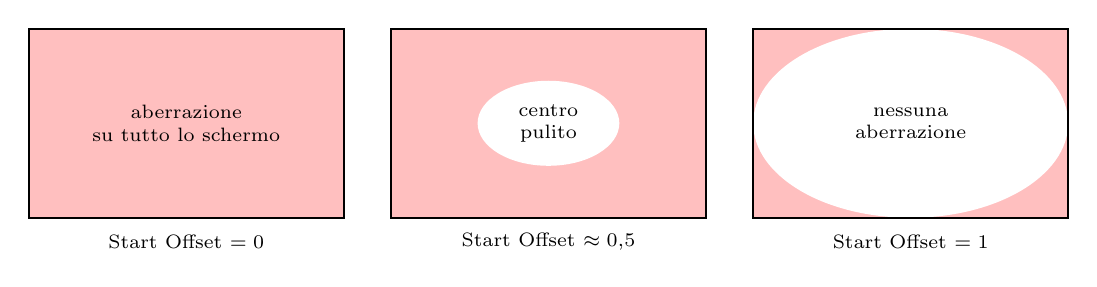
\begin{tikzpicture}[font=\scriptsize, x=1cm, y=1cm]
  \foreach \xs/\r/\lab in {0/0.0/{Start Offset $=0$}, 4.6/0.9/{Start Offset $\approx 0{,}5$}, 9.2/2.0/{Start Offset $=1$}} {
    \begin{scope}[xshift=\xs cm]
      \begin{scope}
        \clip (0,0) rectangle (4,2.4);
        \fill[red!25] (0,0) rectangle (4,2.4);
        \fill[white] (2,1.2) ellipse ({\r} and {\r*0.6});
      \end{scope}
      \draw[thick] (0,0) rectangle (4,2.4);
      \node at (2,-0.3) {\lab};
    \end{scope}
  }
  \node[align=center] at (2,1.2) {aberrazione\\su tutto lo schermo};
  \node[align=center] at (6.6,1.2) {centro\\pulito};
  \node[align=center] at (11.2,1.2) {nessuna\\aberrazione};
\end{tikzpicture}
\caption{Lo Start Offset della Chromatic Aberration: dal centro dello schermo fino al valore
impostato l'immagine resta pulita, oltre compare la separazione dei canali. A 1 l'effetto
sparisce. Ricostruzione schematica.}
\label{ue16:fig:chromatic}
\end{figure}

\paragraph{Approfondimento: aberrazione e accessibilità.} L'aberrazione cromatica imita un
difetto degli obiettivi reali, che non fanno convergere nello stesso punto le diverse
lunghezze d'onda: per questo è più forte ai bordi. Il consiglio del docente coincide con una
pratica diffusa dell'accessibilità: effetti come aberrazione, motion blur, vignettatura forte e
\emph{film grain} affaticano la vista o danno nausea a una parte dei giocatori, e molti giochi
offrono un'opzione per disattivarli. In Unreal si può farlo modificando a runtime le proprietà
del post process (per esempio il \emph{Post Process Settings} di una camera o di un volume da
Blueprint) oppure, per un picco di breve durata come la flashbang, animando l'intensità con una
\emph{Timeline}, lo strumento visto nelle prime lezioni del corso (funzionamento generale
dell'engine). Totten, nel capitolo 5, ricorda che l'horror lavora sull'incertezza percettiva
(l'ombra, la nebbia): l'aberrazione dell'esempio lovecraftiano è la versione
``sullo schermo'' della stessa strategia.

% ---------------------------------------------------------------------
\section{Il Lens Flare}
\label{ue16:sec:flare}

\paragraph{Che cos'è.} ``Questa è un'altra molto comune, molto vista'': ``forse è il tipo di
post-process con cui siamo più familiari'', perché si vede spesso anche nelle immagini delle
fotocamere. È la ``scomposizione dello spettro della luce'': dentro il volume la luce viene
scomposta, e si vedono ``gli esagoni che si creano''. Si può usare ``per diecimila motivi'':
per esempio quando il personaggio è appena uscito all'aperto dopo essere stato al chiuso, e la
scomposizione ``ci accoglie e ci dà un'idea di quanto effettivamente il sole sia forte'', o una
luce in generale.

\paragraph{I parametri.}
\begin{itemize}
  \item \textbf{Intensity}: quanto è forte. ``Se non ricordo male'' è influenzato anche dal
        \textbf{bloom}: ed ``esatto'', aumentando l'intensità del bloom il lens flare diventa
        più sfumato.
  \item \textbf{Tint}: il colore del flare, ``magari prendiamo questo flare violaceo''; si
        può anche modificare a mano il riferimento dei canali RGB.
  \item \textbf{Bokeh Size} (``poke size'': ``sono ignorante su come si pronuncia''): la
        grandezza di ``non lo so neanche come chiamarli, dei cristalli, degli esagoni della
        scomposizione della luce'', per un effetto più o meno scomposto (il docente toglie il
        blu per farlo vedere meglio).
  \item \textbf{Threshold}: ``funziona sempre nello stesso modo'', la soglia minima di
        luminosità per avere l'effetto.
  \item \textbf{Bokeh Shape}: ``devo essere onesto, non ho mai trovato un'utilità a questa
        cosa'', ma si può cambiare la forma dei cristalli con una \textbf{texture}. Quella di
        default si chiama, nella trascrizione, ``Presize default all''; cambiandola si hanno
        cerchi, pentagoni, ``qualsiasi texture abbiamo'': l'icona di un bersaglio, ``un'immaginina
        con delle stelline''. Le texture troppo dettagliate non rendono (``non si nota
        effettivamente il dettaglio''), ma per una questione di forma funzionano; la texture
        porta con sé anche il colore.
  \item \textbf{Tints}: per personalizzare ``al 100\%'' il flare, si può modificare ``ogni
        singolo cristallino'': ce n'è uno viola, uno blu, uno verde, e si decide quali colori
        dello spettro ``risultano maggiormente''. Sono numerati da 0 a 7 (la trascrizione elenca
        ``0, 1, 2, 3, 4, 5, 7'').
\end{itemize}
``Il lens flare lo teniamo, che insomma è piacevole averlo.''

\paragraph{Approfondimento: un difetto che diventa linguaggio.} Il lens flare è un riflesso
interno fra le lenti di un obiettivo, e i suoi esagoni hanno la forma del diaframma; in
Unreal Engine~5 il lens flare del post process è un effetto \emph{image-based}, calcolato a
partire dalle zone più brillanti dell'immagine (per questo dipende dal bloom e dalla soglia),
e la \emph{Bokeh Shape} è appunto la sagoma del diaframma simulato. Nel cinema e nei giochi il
flare comunica ``guardi verso una luce forte'' e, spesso, ``stai guardando attraverso una
camera'': usato ovunque, indebolisce l'idea di una visione in prima persona; usato al momento
giusto, come l'uscita all'aperto del docente, è un segnale di passaggio. Funzionamento generale
dell'engine.

% ---------------------------------------------------------------------
\section{La Depth of Field}
\label{ue16:sec:dof}

\paragraph{Mettere a fuoco.} ``Un'altra cosa molto importante che possiamo utilizzare nel
momento in cui andiamo a fare un render di un'immagine, ma anche quando dobbiamo gestire le
distanze'', è la \textbf{Depth of Field} (la profondità di campo). Permette ``una serie di
modifiche di messa a fuoco'': si modifica la \textbf{distanza focale}, cioè a quale distanza si
mette a fuoco. Nella prova c'è ``una leggera sfocatura'', e più in là ``qualcosa di meno messo a
fuoco, ma comunque non visibilissimo'': ``mettiamo che il nostro personaggio sia vagamente
miope, insomma, vedrà in questo modo qui''.

\paragraph{Gli altri parametri.} Il docente ricorda altri parametri che permettono di
determinare ``la distanza a cui vediamo il blur e l'intensità del blur'': ``quale sia la forza
della sfocatura e da quale distanza venga effettivamente attivata''. Ma ``ricordo funzionasse
in maniera diversa'': ``credo che sulla 4 funzioni in maniera diversa''. Promette di
controllare durante la pausa e di riferire le eventuali modifiche; dopo la pausa, però, la
trascrizione non riporta più nulla sulla depth of field.

\paragraph{Approfondimento: la profondità di campo in Unreal Engine~5.} La differenza che il
docente ricorda c'è davvero. In Unreal Engine~4 esistevano più metodi (\emph{Gaussian},
\emph{Bokeh}, \emph{Circle}), ciascuno con parametri propri come le regioni di transizione
vicina e lontana; in Unreal Engine~5 su PC e console resta di fatto un solo metodo, il
\emph{Cinematic} DOF, i cui parametri principali sono la \emph{Focal Distance} (la distanza
di messa a fuoco, in centimetri), l'\emph{Aperture} o \emph{f-stop} della camera (più è basso,
più la profondità di campo è stretta) e la dimensione del sensore; sono presenti anche
\emph{Depth Blur km for 50\%} e \emph{Depth Blur Radius}, che aggiungono una sfocatura di
distanza indipendente dalla messa a fuoco. Il \emph{Mobile Depth of Field} che il docente vede
nella lista della Camera Actor è la versione semplificata per dispositivi mobili, con distanze
di transizione esplicite, ed è probabilmente il modello di funzionamento che ricordava. Sulla
Camera Actor (\emph{Cine Camera Actor}) la messa a fuoco si regola dalle \emph{Focus Settings},
anche in modo automatico seguendo un actor (funzionamento generale dell'engine). In un gioco
la profondità di campo è utile soprattutto per i menu, i dialoghi e le schermate, dove guida lo
sguardo verso il soggetto: è la stessa funzione che Totten, nel capitolo 7, attribuisce alla
cinematografia, ``attirare l'attenzione del giocatore'' sugli elementi che il designer vuole
fargli vedere.

% ---------------------------------------------------------------------
\section{Il Color Grading}
\label{ue16:sec:grading}

\paragraph{La cosa più famosa.} ``Forse la cosa più famosa per cui è conosciuta e utilizzata
la post-produzione'' è la \textbf{color correction}: applicare all'immagine ``un nuovo stile, un
nuovo tipo di colore'' con una serie di parametri. Il docente richiude tutte le sezioni per
vederle una per una.

\paragraph{Temperature.} ``Di base, il color grading parte dalla \textbf{temperatura}'': una
scena più calda o più fredda, da un estremo all'altro, con ``questa renderizzazione più
giallastra'' o ``completamente sbiancata e bluastra''. Poi la \textbf{tinta} (\emph{Tint}), per
spingere la scena verso il magenta o verso il verde.

\paragraph{Global, Shadows, Midtones, Highlights.} Oltre alla temperatura ci sono i parametri
``che ci permettono di fare una customizzazione più completa'': \textbf{Global},
\textbf{Shadows}, \textbf{Midtones} (``mittons'') e \textbf{Highlights}. Sono la possibilità
di fare color correction su tutta la scena (Global), solo sugli scuri, ``nelle parti più buie,
nelle ombre'' (Shadows), ``nei grigi, nei medi'' (Midtones) e ``nelle luci, nelle parti più
illuminate'' (Highlights) (figura~\ref{ue16:fig:grading}).

\paragraph{Cinque sottoparametri.} ``Funzionano tutti allo stesso modo'': ognuno ha la stessa
lista di \textbf{Saturation}, \textbf{Contrast}, \textbf{Gamma}, \textbf{Gain} e
\textbf{Offset}, da attivare con la spunta ed espandere con la freccia. Con la saturazione si
decide quanto la scena sia satura o desaturata, con lo slider sotto. (A questo punto la
trascrizione si perde per diverse righe in un blocco ripetuto senza senso; quando riprende, il
docente sta parlando del \textbf{contrasto}.) Con il contrasto si gioca sulla differenza ``fra
le luci e le ombre'': la si può accentuare o appiattire, ``una sorta di maschera di contrasto
del colore''. ``Stessa cosa gamma e gain'': moltiplicano la color correction della scena, e si
alzano o abbassano per modificare il colore.

\begin{figure}[htbp]
\centering
\begin{tikzpicture}[font=\scriptsize, x=1cm, y=1cm]
  \shade[left color=black, right color=white] (0,0) rectangle (12,0.7);
  \draw[thick] (0,0) rectangle (12,0.7);
  \draw[thick] (0,1.0) -- (4,1.0);
  \node at (2,1.3) {\textbf{Shadows}: ombre};
  \node at (6,1.3) {\textbf{Midtones}: grigi, medi};
  \node at (10,1.3) {\textbf{Highlights}: luci};
  \draw[thick] (4,0) -- (4,1.1); \draw[thick] (8,0) -- (8,1.1);
  \draw[thick, {Stealth[length=1.6mm]}-{Stealth[length=1.6mm]}] (0,1.8) -- (12,1.8) node[midway, above] {\textbf{Global}: tutta la scena};
  \node[align=center, draw, rounded corners=2pt, fill=gray!10, inner sep=4pt] at (6,-0.9)
    {in ognuna: Saturation $\cdot$ Contrast $\cdot$ Gamma $\cdot$ Gain $\cdot$ Offset};
  \node[align=center, draw, rounded corners=2pt, fill=orange!10, inner sep=4pt] at (6,-1.8)
    {prima, per tutta l'immagine: Temperature (caldo / freddo) e Tint (magenta / verde)};
\end{tikzpicture}
\caption{Le zone del Color Grading. Global agisce su tutta l'immagine, Shadows, Midtones e
Highlights sulle zone scure, medie e chiare; ciascuna ha gli stessi cinque sottoparametri.
I confini fra le zone sono sfumati e regolabili. Ricostruzione schematica.}
\label{ue16:fig:grading}
\end{figure}

\paragraph{Uno strumento avanzato.} ``Il post-process è un elemento molto molto avanzato'':
non perché sia difficile da usare, ``ma nel senso che è difficile ottenere esattamente il
risultato che volete''. È un oggetto con cui ``dovete sperimentare, mettervi là, fare
esperienza'' di come funziona e di quali possibilità ha. ``Se dovessimo esplorarlo al 100\%
ci vorrebbe molto di più di una lezione, e probabilmente non sarei neanche la persona adatta.''
Il docente ha mostrato le lenti ``che potreste utilizzare di più'' per creare un certo
\emph{mood} e un certo tipo di scena; si ferma qui per parlare di altre cose ``ugualmente
importanti'', ``più basilari forse, meno avanzate''. Chi vuole può partire da questa base:
mettere in scena il proprio post process e ``smontarlo un pochino''.

\paragraph{Prima le luci, poi il post process.} La post produzione ``influisce grandemente
sulla luce'': a seconda del tipo di luce in scena si avranno effetti diversi. L'ordine giusto:
prima si costruisce l'illuminazione, ``come abbiamo visto con i light actor qualche lezione
fa'', e solo quando le luci sono posizionate si fa questo lavoro. ``Capisco che è stato molto
brutale e molto rapido'', ma ``più che mostrarvi gli elementi di base e incitarvi a provare a
sperimentare'' non c'è tempo. ``Oggi purtroppo corriamo un po'.''

\paragraph{Approfondimento: colore e significato.} Il color grading di Unreal segue il
modello dei programmi di correzione colore del cinema: Saturation, Contrast, Gamma, Gain e
Offset sono i classici controlli di \emph{lift-gamma-gain} applicati per zone, e i confini
fra Shadows, Midtones e Highlights si regolano con \emph{Shadows Max} e \emph{Highlights Min};
per un controllo totale si può usare una \emph{Color Grading LUT}, una tabella di colori
preparata in un programma esterno (funzionamento generale dell'engine). Totten, nel capitolo 4
(``Basic Color Theory''), fornisce il vocabolario per scegliere: i colori \emph{analoghi}
(tre colori vicini sulla ruota, come blu, blu-viola e viola) creano un'atmosfera armonica e,
in quel caso, ``un senso cupo o freddo''; rosso, rosso-arancio e arancio danno una sensazione
calda; i \emph{complementari} (opposti sulla ruota) creano contrasto. È esattamente il
``posto lugubre'' del docente, caricato di verdi, blu e viola. L'esempio di Totten è
\emph{Bioshock Infinite}: una cappella dominata dal blu in cui le uscite sulla strada
principale sono segnate da elementi complementari, una luce arancione o un fedele in tunica
bianca, mentre i passaggi secondari restano in tinte analoghe. Il color grading regola il
colore dominante; il contrasto che guida il giocatore va poi costruito con le luci e gli
oggetti.

% ---------------------------------------------------------------------
\section{La domanda sull'effetto in due toni}
\label{ue16:sec:duetoni}

\paragraph{La domanda.} Prima di passare al packaging arriva una domanda in chat: ``si possono
applicare effetti di luce più estremi, magari su altri programmi?'' Per esempio ``rendere il
livello in due toni'', ``solo rosso e nero'', per ottenere ``un effetto tipo
\textbf{Limbo}''. ``Sì, si può fare, ma anche già soltanto all'interno di Unreal, utilizzando
un post process volume.''

\paragraph{La zanzara e il cannone.} Il docente sposta però la questione: non è tanto ``se
Unreal lo può fare oppure no'', ma ``per fare quella cosa, è davvero necessario utilizzare
Unreal?'' Se l'idea è creare qualcosa di esteticamente molto semplice, in bianco e nero, si
può forse realizzarlo con altri engine. ``Teniamo sempre a mente che Unreal è un engine pesante
che fa le cose in maniera pesante.'' Se si vuole rifare Limbo, ``che magari è anche in 2D'' e
quindi più semplice, e lo si fa in Unreal, ``stiamo sparando a una zanzara con un cannone'':
``la zanzara l'ammazziamo, però smontiamo pure quello che c'è dietro''. Quanto agli ``altri
programmi'': se si fa un'immagine in Unreal, uno screenshot di un ambiente, e la si modifica
``in post'' con un programma di fotoritocco, ``sì, lo posso fare''.

\paragraph{Mallory.} Lo studente cita un gioco, ``Mallory'' (``Mellori'' più avanti; il nome
esatto non è ricostruibile dalla trascrizione), un titolo per Switch fatto in Unreal, e
condivide dei link. Il docente non lo conosce: ``poi me lo guardo durante la pausa''. In ogni
caso, ``se è fatto in Unreal si può fare tranquillamente'': l'idea stessa del Post Process
Volume è avere un oggetto in scena che permette di passare da un tipo di post produzione a un
altro o di controllarla meglio; ``una volta che mi impratichisco con lo strumento posso fare
un po' quello che mi pare''. Serve però anche gestire bene l'illuminazione: ci si costruisce
l'illuminazione ``come è gestita in quel titolo'' e poi la si modifica a posteriori. (Il
seguito, dopo la pausa, è nella sezione~\ref{ue16:sec:pausa}.)

\paragraph{Approfondimento: scegliere l'engine.} La metafora del cannone tocca un tema di
produzione: il costo di un engine non è solo la licenza, ma il peso dei progetti, i tempi di
compilazione degli shader e del packaging (che il docente sperimenterà di lì a poco) e le
macchine richieste ai giocatori, come ha scoperto lo studente con il portatile che ``non
reggeva''. Per un gioco 2D stilizzato un engine più leggero è spesso la scelta più efficiente;
Unreal ha comunque strumenti 2D (\emph{Paper2D}, gli sprite e i flipbook citati nella lezione
precedente). Un effetto ``in due toni'' in Unreal si ottiene con un \emph{Post Process
Material}: un materiale con dominio \emph{Post Process}, assegnato nei \emph{Rendering
Features} del volume (\emph{Post Process Materials}), che legge il colore della scena e lo
riduce a due colori secondo una soglia di luminosità (funzionamento generale dell'engine).
Totten, nel capitolo 4, usa proprio \emph{Limbo} come esempio di linguaggio visivo: il gioco
gioca il suo stile a silhouette contro le convenzioni del giocatore, come nel puzzle della
pressa in cui il ``pulsante'' rialzato non è il vero meccanismo. Lo stile in due toni, lì, non
è un filtro sopra il gioco: è parte delle regole con cui il giocatore legge lo spazio.

% ---------------------------------------------------------------------
\section{Il packaging: che cos'è e dove si avvia}
\label{ue16:sec:packaging}

\paragraph{Che cos'è.} ``Il packaging è un processo che viene fatto principalmente da Unreal
Engine, in realtà, per cui noi dobbiamo andare a curare soltanto alcune impostazioni.'' È ciò
che ``ci consente di andare a creare un \textbf{eseguibile} con quello che noi abbiamo
all'interno dell'editor''.

\paragraph{Platforms.} Il packaging si avvia dal pulsante \textbf{Platforms} della barra degli
strumenti. Scendendo si vedono ``tutte le varie piattaforme per cui potremmo sviluppare
qualcosa'': \textbf{Android}, \textbf{iOS}, \textbf{Linux}, \textbf{Mac}, \textbf{Windows}.
Accanto ad alcune c'è ``sempre questo segnale di attenzione'': il docente è su Windows, e il
progetto ``non è gestito o pensato'' per funzionare anche sugli altri sistemi. Nella voce
\textbf{Windows} ci sono il \textbf{Package Project}, ``il pulsantone che io premo se voglio far
partire questo processo'', e la scelta della \textbf{configurazione}. ``Queste sono pochissime
impostazioni, e non sono neanche lontanamente tutte quelle che ci servono'': le altre sono nei
\textbf{Project Settings}, la ``macro sezione di setting e di impostazioni per tutto il nostro
progetto'' già vista con Igor (figura~\ref{ue16:fig:packaging}).

\paragraph{Il plugin di Fab.} Un'altra finestra che può servire è quella dei \textbf{Plugins},
che permette di attivare e disattivare i plugin. ``Da quello che so, il plugin di
\textbf{Fab} dà dei problemi con il packaging'': quindi, prima di impacchettare, lo si
disattiva. ``Non so se è stato risolto. Potrebbe essere stato risolto, dovrei informarmi.''

% ---------------------------------------------------------------------
\section{Le impostazioni del progetto}
\label{ue16:sec:impostazioni}

\paragraph{Maps \& Modes.} Nei Project Settings, nella pagina \textbf{Maps \& Modes}, ``oltre
alla Game Mode'', ci sono le \textbf{Default Maps}: \textbf{Editor Startup Map} e
\textbf{Game Default Map}.
\begin{itemize}
  \item L'\textbf{Editor Startup Map} è la mappa con cui si apre l'editor: se la si cambia,
        ``ogni volta che io aprirò questo progetto lui mi partirà da quell'altra mappa'', e per
        tornare al livello di prima bisognerà riaprire a mano la Third Person Map.
  \item La \textbf{Game Default Map} è ``allo stesso modo la mappa di partenza che avremo
        all'interno del nostro eseguibile''. Se il gioco ha un menu che porta alla mappa di
        gioco, non si mette la Third Person Map: ``di solito quello che si fa è mettere un
        \textbf{menu principale}'', o una schermata che, dopo aver cliccato qualche pulsante,
        porta alle mappe che si vogliono giocare.
\end{itemize}
Sono due impostazioni importanti: ``se mai vi capiterà di dire: oddio, dove è andata la mia
mappa, perché si è aperto così, dove sono finito, cosa è successo''; oppure ``per quale motivo
ho fatto il packaging e non mi fa partire da dove dico io'': è la Game Default Map da
modificare. (Il docente scorre altre voci della pagina, ``ma questa non è necessaria'', senza
nominarle.)

\paragraph{Supported Platforms.} Un'altra pagina è quella delle \textbf{Supported Platforms}.
Di default è impostata su \textbf{All Platforms}; togliendo la spunta e lasciando solo ciò che
interessa si può avere, per esempio, soltanto \textbf{Windows} come piattaforma per il
packaging, ``perché il nostro progetto magari non supporta tutti gli altri sistemi
operativi''.

\paragraph{La pagina Packaging.} ``Ultima cosa, ma la più importante'': c'è una pagina tutta
dedicata al \textbf{packaging}. ``Sono un sacco di informazioni, un sacco di parametri'', ma
``la cosa positiva è che la maggior parte di questi parametri sta bene come sta'': non servono
``modifiche assurde''. Alcune voci si vedono subito, altre solo aprendo gli
\textbf{Advanced}. Le prime: \textbf{Build}, ``va bene così'' (l'opzione ``if project has code
or running a locally built editor'', che lascia decidere all'engine se compilare); poi la
\textbf{Build Configuration}.

% ---------------------------------------------------------------------
\section{Le configurazioni di build}
\label{ue16:sec:build}

\paragraph{Cinque configurazioni, tre disponibili.} La \textbf{Build Configuration} decide
``che tipo di configurazione avrà il nostro eseguibile'': \textbf{Debug}, \textbf{DebugGame},
\textbf{Development}, \textbf{Test} e \textbf{Shipping}. ``Per la build che abbiamo scelto''
ne sono attive soltanto tre (le stesse che si ritrovano poi nel menu Platforms: DebugGame,
Development e Shipping). Le differenze (tabella~\ref{ue16:tab:build}):
\begin{itemize}
  \item \textbf{Debug} e \textbf{DebugGame} ``sono modalità di debug'': un eseguibile in cui
        c'è ancora una \textbf{console di comandi} per inserire comandi, fare aggiustamenti,
        ``vedere le linee, vedere quello che sta succedendo, vedere dei text che vengono
        printati''. ``È una versione super di test.''
  \item \textbf{Development} è ``la configurazione di default di Unreal''. Rimuove la maggior
        parte della struttura di debug, aumenta un po' l'ottimizzazione della build, ``ma
        mantiene comunque alcuni strumenti che possono essere utilizzati per il testing''. ``Se
        debug è un eseguibile che può essere di uso a un \textbf{programmatore}, development può
        essere di uso a un \textbf{designer}'': si può ancora modificare qualcosa e usare degli
        input, ma serve soprattutto per testare e poi ritoccare in engine.
  \item \textbf{Shipping} è la modalità ``per la distribuzione'': ``il progetto finito, il
        gioco che le masse giocheranno, si spera le masse''. È ``la versione più ottimizzata
        possibile della build'', ``la build da vendita, praticamente''.
\end{itemize}

\paragraph{Shipping non ottimizza da solo.} ``Aspettate: questo non vuol dire che lui vi
ottimizzi le cose in automatico.'' L'ottimizzazione ``è tutto un discorso a parte, che va fatto
separatamente'': far sì che non ci siano troppe linee di codice, che non ci siano texture a
qualità troppo alta o non utilizzate, eccetera. Shipping ``vuol dire semplicemente che lui va a
togliere tutta una serie di strumenti che non servono più''.

\begin{table}[htbp]
\centering
\small
\begin{tabular}{@{}p{2.3cm}p{5.6cm}p{3.0cm}p{3.1cm}@{}}
\toprule
\textbf{Configurazione} & \textbf{Che cosa contiene (lezione)} & \textbf{Per chi} &
\textbf{Nota} \\
\midrule
Debug & console di comandi, linee, testi stampati: ``versione super di test'' &
programmatore & richiede un progetto con codice C++ \\
DebugGame & come sopra, debug del codice di gioco & programmatore & disponibile \\
Development & default di Unreal; meno debug, un po' più ottimizzata, alcuni strumenti di test
& designer, tester & disponibile; console attiva \\
Test & vicina a Shipping, con qualche strumento di profilazione & QA & richiede codice C++ \\
Shipping & la versione finale, senza strumenti di sviluppo & i giocatori & disponibile; non
ottimizza da sola \\
\bottomrule
\end{tabular}
\caption{Le cinque configurazioni di build. Nel progetto del docente ne sono attive tre; la
colonna ``Nota'' integra con il funzionamento generale dell'engine.}
\label{ue16:tab:build}
\end{table}

\paragraph{Le lingue.} Aprendo gli Advanced si trovano le \textbf{lingue} del packaging
(\emph{Localizations to Package}): ``possiamo andare a selezionare che tipo di lingue dovranno
essere utilizzate''. ``Di default c'è solo l'inglese.'' Se si è localizzato qualcosa, per
esempio perché ci sono già impostazioni e parametri che fanno riferimento a certe lingue, qui
si scelgono quelle da includere.

\paragraph{Approfondimento: le configurazioni secondo Romero e Sewell.} Romero e Sewell, nel
capitolo 12 (``Building and Publishing''), descrivono lo stesso percorso: \emph{Platforms}
$\rightarrow$ piattaforma $\rightarrow$ \emph{Package Project}, la scelta della cartella, la
finestra che avvisa che l'engine sta impacchettando e, in caso di problemi, ``i dettagli
dell'errore nella finestra dell'output log''. Prima, nei \emph{Project Settings}: la pagina
\emph{Description} (nome, miniatura, descrizione del progetto), la pagina \emph{Maps \& Modes}
(``spesso dovrete designare una mappa dedicata al menu principale come prima mappa da
caricare'', e assicurarsi che sia lei a gestire quale mappa si carica dopo) e la pagina della
piattaforma, dove per Windows si cambiano lo \emph{splash screen} e l'\emph{icona}
dell'eseguibile. Sulle configurazioni il libro precisa che nei progetti \emph{solo
Blueprint} le opzioni principali sono \textbf{Development}, che contiene informazioni di debug
utili a trovare errori, e \textbf{Shipping}, ``più pulita'', da usare per la versione da
distribuire; Debug e Test richiedono un progetto con codice C++ (ed è per questo che nel
progetto del docente sono spente). Il libro nomina anche la \emph{Staging Directory}, la
cartella in cui viene salvata la build, l'opzione \emph{For Distribution}, richiesta per
pubblicare su App Store o Google Play, e lo \emph{Zip Project} del menu File, che comprime i
file essenziali del progetto per passarlo a un'altra persona. Una nota importante dello stesso
capitolo: Unreal Engine~5 può creare build Windows solo da Windows e build macOS solo da macOS;
è il ``segnale di attenzione'' che il docente vede accanto alle altre piattaforme.

% ---------------------------------------------------------------------
\section{Le mappe e le cartelle da cucinare}
\label{ue16:sec:cook}

\paragraph{Cook only maps.} ``Fare il packaging di base vuol dire che lui prende tutto il
progetto e lo rende pronto per essere un eseguibile'', con un certo metodo di compressione.
Spuntando \textbf{Cook only maps} (``hook only maps'' nella trascrizione), invece, il
packaging usa ``unicamente le mappe'': si può dirgli di usare soltanto la Third Person Map, e
lui ``si vede cosa c'è dentro'', mette nel pacchetto ``tutto quello che serve per far funzionare''
quella mappa ``e non mette il resto delle cose''.

\paragraph{List of maps to include.} Insieme a Cook only maps serve la voce \textbf{List of maps
to include in a packaged build}. Si aggiunge un elemento, si clicca sui tre puntini e si cerca
la mappa: ``volete level 1, level 2, menu? Magari vi serve il menu''. Nel caso della prova
serve soltanto la Third Person Map (il file \texttt{.umap}): ``non serve andare a inserire anche
il build data'' (il file \texttt{\_BuiltData}) ``o lo \texttt{.uasset}''. Si possono aggiungere
altre mappe, copiarle, eliminarle.

\paragraph{Directories to never cook.} ``Un'altra cosa che ci torna utile'' è
\textbf{Directories to never cook}: le cartelle che non devono mai finire nel pacchetto. Si
aggiunge un elemento (``un index zero'') e si sceglie la cartella. Gli esempi:
\begin{itemize}
  \item ``nulla di \emph{GameApps}'' (il nome della cartella, nella trascrizione, è ``game
        apps'') ``deve finire dentro il packaging'';
  \item una cartella con ``tutta una serie di modelli 3D molto fighi'' che non si è riusciti a
        inserire e che magari si vogliono usare in un \textbf{DLC} più avanti.
\end{itemize}
I motivi sono due. Il primo è il \textbf{data mining}, ``diventato super popolare adesso'': i
file messi nel gioco ``possono essere ritrovati da chi va a scavare''. Il secondo: sono comunque
cose ``che vanno ad essere cucinate e vengono comunque inserite all'interno della build''.
Togliere le cartelle che non servono ``ci fa risparmiare giga'': un progetto più piccolo e più
semplice da gestire (tabella~\ref{ue16:tab:packaging}).

\begin{table}[htbp]
\centering
\small
\begin{tabular}{@{}p{4.6cm}p{2.8cm}p{6.6cm}@{}}
\toprule
\textbf{Impostazione} & \textbf{Dove} & \textbf{A che cosa serve} \\
\midrule
Package Project, configurazione & Platforms $\rightarrow$ Windows & avviare il packaging;
scegliere DebugGame, Development, Shipping o le impostazioni del progetto \\
Plugin di Fab & Edit $\rightarrow$ Plugins & disattivarlo prima del packaging (problemi
noti, forse risolti) \\
Editor Startup Map & Maps \& Modes & la mappa con cui si apre l'editor \\
Game Default Map & Maps \& Modes & la prima mappa dell'eseguibile: di solito il menu \\
Supported Platforms & Project Settings & limitare le piattaforme (per esempio solo Windows) \\
Build & Packaging & lasciare il default \\
Build Configuration & Packaging & Debug, DebugGame, Development, Test, Shipping \\
Localizations to Package & Packaging (Advanced) & le lingue incluse; default inglese \\
Cook only maps & Packaging (Advanced) & impacchettare solo ciò che serve alle mappe elencate \\
List of maps to include & Packaging (Advanced) & le mappe (\texttt{.umap}) da includere \\
Directories to never cook & Packaging (Advanced) & cartelle escluse: asset scartati, DLC,
spazio \\
Show Output Log & finestra del packaging & seguire il processo e trovare gli errori in rosso \\
\bottomrule
\end{tabular}
\caption{Le impostazioni del packaging viste a lezione, nell'ordine in cui il docente le
mostra.}
\label{ue16:tab:packaging}
\end{table}

\paragraph{Approfondimento: che cosa vuol dire ``cucinare''.} Il \emph{cooking} è la fase in
cui l'engine converte gli asset dal formato dell'editor a quello ottimizzato per la
piattaforma di destinazione: compila gli shader, comprime le texture, elimina i dati che
servono solo all'editor. Il packaging vero e proprio raccoglie poi gli asset cucinati in
archivi (\emph{.pak}, o \emph{IoStore} in Unreal Engine~5) accanto all'eseguibile. Con Cook
only maps disattivato l'engine cucina di norma tutto il contenuto del progetto, compresi gli
asset mai usati; con l'opzione attiva segue le \emph{reference} a partire dalle mappe
elencate. Un'avvertenza: un asset caricato solo per nome, a runtime (per esempio con un
percorso scritto in una stringa), non è una reference visibile al cook e rischia di restare
fuori; per questi casi esistono le voci \emph{Additional Asset Directories to Cook}. Anche
\emph{Directories to never cook} va usata con attenzione: se un asset escluso è referenziato
da una mappa inclusa, il cook segnala un errore o il gioco lo perde (funzionamento generale
dell'engine). Totten, nel capitolo 2, parla di \emph{modular design} e di ``schedule'' dei
pezzi di un livello: sapere fin dalla pre-produzione quali pezzi servono rende più facile
anche sapere, alla fine, che cosa lasciare fuori.

% ---------------------------------------------------------------------
\section{L'avvio del packaging e l'Output Log}
\label{ue16:sec:avvio}

\paragraph{Dove salvare.} Per avviare si torna al menu Platforms: lì si vedono le
configurazioni (``debug'', \textbf{Development} e \textbf{Shipping}, ``perché sono le tre
possibili''), oppure \emph{Use Project Setting}, cioè quelle della pagina Packaging. Il docente
sceglie \textbf{Development}. Con \textbf{Package Project} si apre una finestra che chiede dove
creare il pacchetto; il docente sceglie il desktop, e parte il processo, accompagnato da un
``suonino''.

\paragraph{La prima volta è lenta.} ``Fare un packaging la prima volta è molto lento'', anche
se è solo di una mappa. ``Dopo il primo packaging diventa tutto molto più veloce.'' Mentre
lavora (``parte \emph{Cancel}, chiaramente'', per interromperlo) si può aprire lo
\textbf{Show Output Log}: lì si vede tutto quello che sta succedendo. Scorrendolo (``con la
rotella del mio mouse che è rotta è tremendo'') si controlla se va tutto bene, se ci sono
errori o ``piccoli problemi'', o cose che creano problemi al packaging. In quel momento
l'engine sta facendo ``la compilazione degli shader''.

\paragraph{La scritta rossa.} ``Arriverà un punto in cui magari c'è una scritta rossa.'' La
scritta rossa ``vuol dire che c'è un problema che gli impedisce di fare il packaging''. Si legge
che cosa dice, si risolve quel problema, e si riprova.

\paragraph{Che cosa esce.} Se il processo finisce, nella cartella scelta si crea una cartella
che, ``se non gli viene dato un nome'', si chiama \textbf{Windows No Editor} (in Unreal
Engine~5 è semplicemente \emph{Windows}; \emph{WindowsNoEditor} era il nome di Unreal
Engine~4). Dentro c'è l'\textbf{eseguibile}: avviandolo parte il progetto, che in questo caso
sarebbe soltanto la Third Person Map, ``perché è l'unica mappa che gli abbiamo detto di
cucinare''. Il personaggio spawna sul \textbf{Player Start} e può andare in giro: ``non c'è un
obiettivo, non c'è una fine, non c'è nulla''.

\paragraph{I confini della mappa.} ``Chiaramente, per un packaging, non dovrebbero esserci
posti in cui puoi buttarti di sotto nel nulla, come il bordo della mappa''; né posti ``in cui
io non voglio che i giocatori vadano''. Nessuna domanda sul packaging. Siccome ci vorrà ``un
po' troppo tempo'', il docente anticipa la pausa, ``in modo che forse durante la pausa lui
finisca di calcolare'' e si possa vedere che cosa genera. Dopo la pausa: ``un paio di altri
attori'' utili quando si fa un livello, il Blueprint delle \textbf{spline}, ``che potete
utilizzare per un sacco di elementi diversi'', e, ``se ci avanza un po' di tempo'', le
\textbf{decal}, ``un altro strumento di decoro, di arredo'' per aggiungere dettagli in giro per
la mappa. ``Facciamo un 15 minuti di stop. Ci rivediamo alle 5 e mezza.''

\begin{figure}[htbp]
\centering
\begin{tikzpicture}[font=\scriptsize, x=1cm, y=1cm,
  ue16step/.style={draw, thick, rounded corners=2pt, fill=white, align=center, text width=2.6cm, minimum height=1.1cm, inner sep=3pt},
  ue16arr/.style={-{Stealth[length=1.8mm]}, thick}]
  \node[ue16step, fill=gray!10] (a) at (0,0) {Plugins:\\disattivare Fab};
  \node[ue16step, fill=blue!8] (b) at (3.3,0) {Maps \& Modes:\\Game Default Map\\(il menu)};
  \node[ue16step, fill=blue!8] (c) at (6.6,0) {Packaging:\\configurazione,\\lingue, mappe,\\cartelle escluse};
  \node[ue16step, fill=orange!12] (d) at (9.9,0) {Platforms $\rightarrow$\\Windows $\rightarrow$\\Package Project};
  \node[ue16step, fill=red!8] (e) at (9.9,-2.2) {Output Log:\\shader, cook;\\scritte rosse?};
  \node[ue16step, fill=green!12] (f) at (6.6,-2.2) {cartella \emph{Windows}\\con l'eseguibile};
  \node[ue16step, fill=green!12] (g) at (3.3,-2.2) {ritestare il gioco\\impacchettato};
  \node[ue16step, fill=green!12] (h) at (0,-2.2) {caricare (itch.io,\\Drive) e link\\su Discord};
  \draw[ue16arr] (a) -- (b); \draw[ue16arr] (b) -- (c); \draw[ue16arr] (c) -- (d);
  \draw[ue16arr] (d) -- (e); \draw[ue16arr] (e) -- (f); \draw[ue16arr] (f) -- (g);
  \draw[ue16arr] (g) -- (h);
  \draw[ue16arr, red!70!black] (e.east) -- ++(0.6,0) |- node[pos=0.25, right, align=left] {errore:\\risolvere\\e ripartire} (d.east);
\end{tikzpicture}
\caption{Il percorso del packaging come emerge dalla lezione, fino al consiglio finale di
ritestare il gioco impacchettato e condividerlo. Ricostruzione schematica.}
\label{ue16:fig:packaging}
\end{figure}

% ---------------------------------------------------------------------
\section{La pausa e Mallory}
\label{ue16:sec:pausa}

\paragraph{Il packaging non finisce.} Durante la pausa la trascrizione contiene soltanto il
blocco ripetuto già visto, che non appartiene alla lezione. Alla ripresa: ``purtroppo noi ci
siamo, ma Unreal ancora no, ancora non ho finito col packaging''. Il docente lo interrompe,
``perché sennò mi impedisce di fare altre robe'': ``non pensavo ci volesse così tanto tempo''.
Il risultato del packaging, quindi, non viene mostrato.

\paragraph{Mallory, visto.} Il docente ha guardato il gioco segnalato prima. ``Sembra molto
carino'': non l'ha potuto giocare, ma dal video ``sembra un platform simpatico con un bell'ambiente''.
Non gli è sembrato che ci sia ``un eccessivo utilizzo del post-process''. Quello che fanno
``sicuramente'' è cambiare il modo in cui vengono renderizzate luci e ombre: ``ci sono delle parti
con le ombre che sono molto rossastre rispetto alla luce, che magari è una luce più neutra'',
``una piccola vignettatura'' e ``un effetto di sfocatura messa davanti alla camera''. Lo
studente ha in mente anche altri titoli; il docente osserva che il genere platform ``ora come ora
è messo in mano agli indipendenti'': ``non ci sono più grossi titoloni che fanno quel tipo di
roba''. È giusto cercare ``cose carine fatte da persone in giro'', su Twitch o fra i piccoli
titoli su Steam. ``Purtroppo non è proprio il mio genere'', a parte ``i vecchi classiconi PS1,
PS2''.

\paragraph{Come rifare quell'effetto.} Le indicazioni del docente:
\begin{itemize}
  \item una \textbf{Dirt Mask}, come effetto di camera: una texture sovrapposta alla lente. Fra
        le texture del progetto non ce n'è una adatta; una ``un po' più fitta'' dà già ``questa
        specie di effetto statico, tra virgolette, sulla camera'', da gestire poi con i colori
        corretti (quella provata rende la Dirt Mask rossa: ``se riesci a fartela di effetto
        statico perfetto, potrebbe non essere male'');
  \item negli \textbf{Image Effects}, una piccola \textbf{vignettatura} (\emph{Vignette
        Intensity}), che ``va a scurire lo schermo'' nelle parti esterne e dà ``già di base'' un
        mood un po' più scuro;
  \item il resto ``è tutta \textbf{color correction}'': modificare i colori delle ombre per
        avvicinarli a quelli delle luci, desaturare un po' la scena (``c'è fondamentalmente una
        scala di grigio e in più c'è il rosso, barra rosa'') e mettere ``un accento sul rosso''
        dove c'è il rosso.
\end{itemize}

\paragraph{Monument Valley.} Mallory ricorda al docente, per la struttura dei livelli ``molto
geometrici, molto quadratosi'', i \textbf{Monument Valley}: ``non sono dei platform, sono dei
puzzle game misto opera estetica''. Si basano sull'\textbf{illusione ottica}: il personaggio
``cammina su un corridoio e poi improvvisamente inizia a camminare sulla parete e poi passa
dietro la scena'', e bisogna ruotare il livello per capire dove sta andando. ``Faccio fatica a
descriverli, però cercali, sono molto carini.'' Poi si torna al programma: ``post process,
rapidamente e bruttamente, ma lo abbiamo visto''.

\paragraph{Approfondimento: accentare un colore.} L'``accento sul rosso'' in una scena
desaturata è un'applicazione diretta del contrasto di Totten (capitolo 4): un elemento di un
colore diverso dal dominante attira l'attenzione, e se il colore è sempre lo stesso diventa un
segnale che il giocatore impara a leggere. In Unreal non c'è un controllo per ``desaturare
tutto tranne il rosso'' nel color grading standard: lo si ottiene con un Post Process Material
o, più semplicemente, desaturando con il post process e dando agli oggetti rossi materiali con
un po' di \emph{emissive}, così che restino saturi anche dopo la correzione. La vignettatura si
regola con \emph{Vignette Intensity} negli \emph{Image Effects}; la Dirt Mask nella sezione
\emph{Lens}, con \emph{Dirt Mask Texture}, \emph{Intensity} e \emph{Tint}, ed è visibile solo
dove c'è bloom (funzionamento generale dell'engine). Totten, nel capitolo 4, nota anche come
le associazioni dei colori passino nei giochi: rosso e verde per la salute, blu per la magia.

% ---------------------------------------------------------------------
\section{Le spline: che cosa sono}
\label{ue16:sec:spline}

\paragraph{Una linea.} Il docente ha preparato due Blueprint ``al volo prima di cominciare la
lezione''. Prima, però, ``che cos'è una spline?'' È un \textbf{component} che si può aggiungere
ai Blueprint, ma ``in realtà è proprio un tipo di oggetto'' con una funzione ben specifica, che
si usa anche per modificare il funzionamento del \textbf{landscape} (le \emph{landscape
spline}). Il docente crea un Blueprint di prova con un \textbf{Spline Component}; il tooltip
dice che è ``una spline shape che può essere usata per altri scopi, tipo animare oggetti''.
``È una linea, fondamentalmente.''

\paragraph{Punti e tangenti.} Messa in scena, la spline ``non è nient'altro che una linea'' che
si può allungare, curvare e arricchire di punti (figura~\ref{ue16:fig:spline}):
\begin{itemize}
  \item all'inizio ha \textbf{due punti}, l'inizio e la fine;
  \item cliccando sul punto finale compaiono altri due punti, la \textbf{tangente}; spostandola,
        la spline si curva;
  \item per creare \textbf{nuovi punti} si fa come quando si copia un oggetto: sulla freccia
        del gizmo, \textbf{Alt} premuto, si trascina, ``e ho fatto una copia''; ogni punto
        nuovo curva la linea, si può alzare, spostare, fino a costruire ``una figura, una
        struttura'';
  \item con il tasto destro, \textbf{Delete Spline Point} elimina un punto (la spline si
        riempie da sola fra i punti rimasti, ``lui autofilla'') e \textbf{Add Spline Point
        Here} ne aggiunge uno.
\end{itemize}

\begin{figure}[htbp]
\centering
\begin{tikzpicture}[font=\scriptsize, x=1cm, y=1cm]
  \draw[very thick, blue!70!black] (0,0) .. controls (2,0) and (2.5,2) .. (4.5,2)
                                   .. controls (6.5,2) and (6.5,0) .. (8.5,0.3)
                                   .. controls (10,0.5) and (10.5,1.6) .. (11.5,1.8);
  \foreach \p/\n in {(0,0)/0, (4.5,2)/1, (8.5,0.3)/2, (11.5,1.8)/3} {
    \fill[white, draw=black, thick] \p circle (3pt);
    \node[below=4pt] at \p {punto \n};
  }
  % tangente sul punto 1
  \draw[thick, red!70!black, {Stealth[length=1.5mm]}-{Stealth[length=1.5mm]}] (2.9,2) -- (6.1,2);
  \fill[red!70!black] (2.9,2) circle (2pt); \fill[red!70!black] (6.1,2) circle (2pt);
  \node[above, red!70!black] at (4.5,2.1) {tangente: lunghezza e verso curvano la linea};
  \node[align=left, anchor=west] at (0,-1.1) {Alt + trascinamento su un punto: nuovo punto \quad
    tasto destro: Add Spline Point Here, Delete Spline Point};
  \node[align=left, anchor=west] at (0,-1.6) {segmenti = punti $-$ 1 (qui 4 punti, 3 segmenti: indici da 0 a 2)};
\end{tikzpicture}
\caption{Una spline con quattro punti. Ogni punto ha una posizione e una tangente; i segmenti
sono uno in meno dei punti. Ricostruzione schematica.}
\label{ue16:fig:spline}
\end{figure}

% ---------------------------------------------------------------------
\section{A che cosa servono le spline}
\label{ue16:sec:usi}

\paragraph{Il muro di spine.} ``Immaginate di poter piazzare un oggetto lungo questa linea, o
di poter modellare un oggetto lungo questa linea.'' La storia che il docente racconta gli è
successa ``quando stavo in Accademia'', quando aveva cominciato a ``smanettare con questo
strumentino''. Bisogna creare un \textbf{muro di spine}, come nella \emph{Bella addormentata
nel bosco}, ``tutte le spine attorno al castello''. Due strade:
\begin{itemize}
  \item andare dall'``amico grafico'' e chiedergli ``un muro di spine fatto così, così e così'':
        una mesh ``non particolarmente impegnativa'', ma che richiede tempo e che, se va
        modificata, deve tornare in un software di modellazione come \textbf{Blender} o
        \textbf{Maya};
  \item ``una roba un po' più intelligente'': farsi creare soltanto un \textbf{cilindro di
        spine} e \emph{replicarlo} lungo una spline, così che la mesh ``viene ricreata e viene
        modificata sulla base della spline'', seguendone l'andamento.
\end{itemize}

\paragraph{Altri usi.} ``Al di là di questa cosa'', la struttura serve per molte cose: una
\textbf{pista} per un gioco di macchine (``vi create un blueprint di spline con la strada''); un
\textbf{muro} più stondato nel blockout o nella gym, per esempio ``che sale a spirale verso
l'alto'', quando ``non avete nulla che ve lo fa fare in maniera comoda''. Il docente lo mostra
``in due forme, in due versioni'': una ``più semplice e più brutta'', l'altra ``un po' più
funzionale''. I Blueprint si chiamano \textbf{Spline by Length} e \textbf{Spline by Point}.

\paragraph{La mesh del tubo.} Per la prova usa un tubo, ``un oggetto molto semplice'' che è
anche nel progetto degli studenti: \textbf{SM\_PipeSplineBody} (``Sm pipe spline body''). Il
docente prima dice che ``non è fatto benissimo per essere un oggetto da spline'', poi si
corregge: ``ho detto una cazzata, l'avevo vista in maniera veloce prima''. Funziona bene
perché è \textbf{segmentato}: ha i suoi triangoli e ``questa spezzatura in orizzontale'', è
\textbf{modulare} (``cilindro, cilindro, cilindro''). Questo permette al Blueprint di
replicarlo ``senza andarlo a spezzare'', perché la struttura del tubo viene replicata cilindro
per cilindro. Nella prima versione, allungando la spline il cilindro si allunga; piegandola,
si piega ``però si spezza'', perché è fatta ``in una maniera meno ottimale''; nella seconda ``si
spacca'' ancora, ma ``dovrebbe notarsi di meno''. La differenza (figura~\ref{ue16:fig:pointlength}):
``il primo blueprint, by point, \emph{stretcha} l'oggetto; questo invece ricrea l'oggetto per
lunghezza, quindi è un pochino più fedele''.

\begin{figure}[htbp]
\centering
\begin{tikzpicture}[font=\scriptsize, x=1cm, y=1cm]
  % by point
  \node[anchor=west] at (0,2.9) {\textbf{Spline by Point}: una mesh per ogni segmento, stirata fino al punto successivo};
  \foreach \a/\b/\c in {0/4.2/blue!20, 4.2/6.2/green!20, 6.2/12/orange!20} {
    \draw[thick, fill=\c] (\a,1.6) rectangle (\b,2.4);
  }
  \foreach \x in {0,4.2,6.2,12} \fill[black] (\x,2.0) circle (2.2pt);
  \node at (2.1,2.0) {stirata}; \node at (5.2,2.0) {schiacciata}; \node at (9.1,2.0) {molto stirata};
  % by length
  \node[anchor=west] at (0,1.0) {\textbf{Spline by Length}: una mesh ogni \emph{Mesh Length}, sempre proporzionata};
  \foreach \i in {0,...,5} {
    \draw[thick, fill=blue!20] ({\i*2},-0.2) rectangle ({\i*2+2},0.6);
  }
  \foreach \x in {0,12} \fill[black] (\x,0.2) circle (2.2pt);
  \draw[{Stealth[length=1.4mm]}-{Stealth[length=1.4mm]}] (0,-0.45) -- (2,-0.45) node[midway, below] {Mesh Length (250)};
  \node[align=center] at (9,-0.7) {anche con due soli punti: tanti pezzi quanti\\ne stanno nella lunghezza della spline};
\end{tikzpicture}
\caption{Le due versioni del Blueprint su una spline dritta. Per punto, il numero di mesh è
uno in meno dei punti e ciascuna si deforma fino al punto successivo; per lunghezza, il numero
di mesh dipende dalla lunghezza della spline divisa per quella della mesh. Ricostruzione
schematica.}
\label{ue16:fig:pointlength}
\end{figure}

% ---------------------------------------------------------------------
\section{Il Blueprint per punto}
\label{ue16:sec:bypoint}

\paragraph{La struttura.} Nel \textbf{Spline by Point} la viewport contiene la spline e
``un oggetto che poi gli abbiamo attaccato con un nodo''; l'Event Graph è vuoto, e tutto è nel
\textbf{Construction Script}. ``È una struttura abbastanza semplice'', usabile ``tranquillamente''
per un lavoro di blockout, ``di prototipazione''. Alcune cose il docente le fa ``un po' più
veloce, perché probabilmente le avete già viste anche con Igor''. Il grafo
(figura~\ref{ue16:fig:grafopoint}):
\begin{enumerate}
  \item un \textbf{For Loop}, ``perché dobbiamo loopare un oggetto''. Il \emph{First Index} è
        \textbf{0}, ``la base dell'indice''. Il \emph{Last Index} viene dal numero di punti della
        spline, preso trascinando la spline nel grafo e usando \textbf{Get Number of Spline
        Points}; al numero si \textbf{sottrae 2}. Il motivo detto a lezione: ``sono i due punti
        che abbiamo già di base, l'inizio e la fine'', che ``non ci interessano per il
        calcolo'' (vedi l'approfondimento più sotto per la ragione esatta);
  \item dal corpo del loop, \textbf{Add Spline Mesh Component}, con ``tutta una serie di
        parametri'': soprattutto la \textbf{Static Mesh} da usare (qui SM\_PipeSplineBody), i
        materiali, \emph{Start Position}, \emph{Start Tangent}, \emph{End Position}, \emph{End
        Tangent} e il \textbf{Forward Axis};
  \item \textbf{Set Start and End}, che dà al componente l'inizio e la fine come punti di
        riferimento;
  \item \textbf{Attach Component to Component}, che attacca il componente creato al Blueprint,
        con il \textbf{Default Scene Root} come \emph{parent};
  \item due nodi \textbf{Get Location and Tangent at Spline Point}, con la spline come target:
        il primo con l'indice del loop (posizione e tangente di partenza), il secondo con
        l'indice \textbf{più 1} (``il punto successivo''), per la fine. ``In questo modo lui, fra
        punti, va a creare una replica del nostro oggetto.''
\end{enumerate}

\begin{figure}[htbp]
\centering
\begin{tikzpicture}[font=\scriptsize, x=1cm, y=1cm,
  ue16node/.style={draw, thick, rounded corners=2pt, fill=white, align=center, minimum height=0.6cm, inner sep=3pt},
  ue16fn/.style={ue16node, fill=yellow!15},
  ue16ex/.style={ue16node, fill=blue!10},
  ue16arr/.style={-{Stealth[length=1.6mm]}, thick},
  ue16data/.style={-{Stealth[length=1.4mm]}, thin, dashed}]
  \node[ue16ex] (cs) at (0,0) {Construction\\Script};
  \node[ue16ex] (loop) at (2.6,0) {For Loop\\First 0};
  \node[ue16fn] (num) at (2.6,-1.8) {Get Number of\\Spline Points $-$ 2};
  \node[ue16ex] (add) at (5.6,0) {Add Spline Mesh\\Component\\(Mesh, Forward Axis)};
  \node[ue16ex] (sse) at (8.9,0) {Set Start\\and End};
  \node[ue16ex] (att) at (11.8,0) {Attach Component\\to Component\\(parent: Root)};
  \node[ue16fn] (g1) at (6.2,-2.0) {Get Location and Tangent\\at Spline Point (Index)};
  \node[ue16fn] (g2) at (9.9,-2.0) {Get Location and Tangent\\at Spline Point (Index + 1)};
  \draw[ue16arr] (cs) -- (loop); \draw[ue16arr] (loop) -- node[above] {Body} (add);
  \draw[ue16arr] (add) -- (sse); \draw[ue16arr] (sse) -- (att);
  \draw[ue16data] (num) -- node[left] {Last Index} (loop);
  \draw[ue16data] (loop.south east) -- (g1.north west);
  \draw[ue16data] (g1.north) -- node[left, pos=0.4] {Start Pos., Tangent} (sse.south west);
  \draw[ue16data] (g2.north) -- node[right, pos=0.4] {End Pos., Tangent} (sse.south east);
\end{tikzpicture}
\caption{Il Construction Script del Blueprint \emph{Spline by Point}. Le frecce continue
sono il flusso di esecuzione, quelle tratteggiate i dati. Ricostruzione dai nodi nominati a
lezione.}
\label{ue16:fig:grafopoint}
\end{figure}

\paragraph{Il Forward Axis.} Il docente cambia la mesh con un muro modulare (cerca
``modulare'' nel Content), compila, salva, e il risultato non è quello voluto: ``lo sta
replicando'', ma non come si vorrebbe. Il motivo è il \textbf{Forward Axis}: ``qual è l'asse
frontale dell'oggetto, qual è l'asse allineato con la spline''. Per il tubo era rimasto su
\textbf{X}, ed era giusto: aprendo la mesh, il gizmo mostra che il tubo è allineato con l'asse
X (``Z sono verticali, l'asse delle Y va in questa direzione''), e il tubo deve allungarsi
proprio lungo X. Per il muro il docente prova \textbf{Y} (``presumo''), ottiene un muro da
abbassare e si confonde (``aspetta, la stessa Y, sono confuso''); alla fine il muro funziona con
l'asse \textbf{Z}, ``forse per come era stato costruito''. ``Questo è probabilmente anche il fatto
che lui non è fatto per fare questa roba.''

\paragraph{Lo stretch.} Con il muro si possono fare ``le pareti di una stanza'', ruotare,
modificare; ``tuttavia, ogni volta che io lo modifico, il muro si \emph{stretcha}''. Il muro
``non la sta prendendo benissimo'', perché non è pensato per essere modellato così: servono
mesh adatte. Il docente prova con un \textbf{cubo}: ``l'effetto non è gradevolissimo perché viene
stretchato'', ma permette già ``una specie di blockout più o meno preciso''. ``Chiaro questo
discorso?'' Nessuna domanda. Il Blueprint costruisce la spline ``sulla base del numero di punti''
e la si rialza perché i pezzi siano tutti allo stesso livello.

% ---------------------------------------------------------------------
\section{Il Blueprint per lunghezza}
\label{ue16:sec:bylength}

\paragraph{La differenza, vista.} ``Cosa succede se andiamo invece a strutturare questa cosa
per lunghezza, per segmenti?'' In teoria si ha ``un po' più di controllo''. Il docente mette le
due versioni una accanto all'altra con il muro di prima (asse Z), ``soltanto dritte per dritte
avanti'', senza curve. Nella versione \textbf{by point} ogni nuovo punto genera una nuova mesh,
ma ``questa mesh può anche essere stretchata'': allungando, si allunga. Nella versione
\textbf{by length} ``la mesh sarà sempre proporzionata'': tirando la spline, ``anche se abbiamo
soltanto due punti, il muro rimane replicato in maniera corretta''. Il muro ``si spacca'' nelle
curve, ``perché non è pensato per fare le curve in questo modo''.

\paragraph{Attenzione ai poligoni.} ``State attenti a come utilizzate questa cosa, perché state
andando a generare un sacco di mesh'': ``state aggiungendo un sacco di poligoni''.

\paragraph{Il grafo.} ``La struttura finale è la stessa dello spline by point'': For Loop,
Add Spline Mesh Component, Set Start and End, Attach Component to Component. Cambia come si
calcolano l'indice e i punti (figura~\ref{ue16:fig:grafolength}):
\begin{enumerate}
  \item una variabile \textbf{float} con la lunghezza su cui replicare l'oggetto: ``ogni tot di
        quella lunghezza, replica l'oggetto''. Il docente l'aveva chiamata \emph{SplineLength},
        e durante la spiegazione la rinomina \textbf{MeshLength}, ``che ha più senso''. Il suo
        valore deve essere uguale al lato della mesh che si ``stretcha''. Era a 186, e il muro
        risultava ``più piccolo di come dovrebbe essere''; la mesh del muro ha una
        \emph{Approx Size} di \textbf{71 $\times$ 250 $\times$ 250}, ``quindi, essendo un
        quadrato, a noi serve 250''. Con 250 il muro torna proporzionato. (Il docente toglie
        anche tre nodi rimasti dalla versione precedente, ``che non ci servono più'');
  \item \textbf{Get Spline Length} dalla spline: la lunghezza della linea, $x$. La si
        \textbf{divide} per MeshLength: ``in quante componenti verrebbe suddivisa la spline per
        mesh''. ``Sappiamo che la nostra mesh è lunga 10, la nostra spline è lunga 100: ci saranno
        10 pezzi.'' Il risultato va nel \emph{Last Index} del loop, passando per un
        \textbf{Truncate}, ``messo come nodo automatico'' per convertire da float a integer;
  \item al posto di Get Location and Tangent at Spline Point, due coppie di nodi:
        \textbf{Get Location at Distance Along Spline} e \textbf{Get Tangent at Distance Along
        Spline} (``a noi serve la location o la tangente a un punto di distanza lungo la
        spline''). La \textbf{distanza} di partenza è l'indice moltiplicato per MeshLength; quella
        di arrivo è l'indice \textbf{più 1}, moltiplicato per MeshLength;
  \item un \textbf{Clamp} sulla tangente, con massimo la lunghezza della mesh. La tangente
        ``cresce sulla base della distanza dal punto successivo'' e ``ruota la struttura'':
        senza clamp, ``per questo calcolo cresce all'infinito'';
  \item tutto si ricollega a Set Start and End: \emph{Start Position}, \emph{Start Tangent},
        \emph{End Position}, \emph{End Tangent}. ``Questo ci permette di aggiornare e
        modificare la mesh sulla base della distanza, quindi sulla base di quanto è lunga la
        spline.''
\end{enumerate}

\begin{figure}[htbp]
\centering
\begin{tikzpicture}[font=\scriptsize, x=1cm, y=1cm,
  ue16node/.style={draw, thick, rounded corners=2pt, fill=white, align=center, minimum height=0.6cm, inner sep=3pt},
  ue16fn/.style={ue16node, fill=yellow!15},
  ue16par/.style={ue16node, fill=green!10},
  ue16ex/.style={ue16node, fill=blue!10},
  ue16data/.style={-{Stealth[length=1.4mm]}, thin}]
  \node[ue16fn] (len) at (0,0.7) {Get Spline\\Length};
  \node[ue16par] (ml) at (0,-0.7) {MeshLength\\(float, 250)};
  \node[ue16node] (div) at (2.5,0) {Divide};
  \node[ue16node] (tr) at (4.3,0) {Truncate};
  \node[ue16ex] (loop) at (6.5,0) {For Loop\\0 -- Last Index};
  \node[ue16node] (m1) at (9.4,1.2) {Index $\times$ MeshLength};
  \node[ue16node] (m2) at (9.4,-1.2) {(Index + 1) $\times$ MeshLength};
  \node[ue16fn] (gs) at (9.4,2.9) {Get Location / Tangent at Distance Along Spline\\(inizio del pezzo)};
  \node[ue16fn] (ge) at (8.6,-2.9) {Get Location / Tangent at Distance Along Spline\\(fine del pezzo)};
  \node[ue16node] (cl) at (13.6,0) {Clamp delle\\tangenti\\(max MeshLength)};
  \node[ue16ex] (sse) at (13.6,-2.9) {Set Start\\and End};
  \draw[ue16data] (len) -- (div); \draw[ue16data] (ml) -- (div);
  \draw[ue16data] (div) -- (tr); \draw[ue16data] (tr) -- (loop);
  \draw[ue16data] (loop) |- (m1); \draw[ue16data] (loop) |- (m2);
  \draw[ue16data] (m1) -- node[right] {distanza} (gs); \draw[ue16data] (m2.south) -- node[right] {distanza} (m2.south |- ge.north);
  \draw[ue16data] (gs.east) -| node[pos=0.75, right, align=left] {posizione\\e tangente} (cl.north);
  \draw[ue16data] (ge.east) -- node[above, align=center] {posizione,\\tangente} (sse.west);
  \draw[ue16data] (cl.south) -- node[right, align=left] {Start Position,\\Start/End Tangent} (sse.north);
\end{tikzpicture}
\caption{La parte di calcolo del Blueprint \emph{Spline by Length}. Il numero di ripetizioni
è la lunghezza della spline divisa per quella della mesh; ogni pezzo va dalla distanza
$i \cdot L$ alla distanza $(i+1) \cdot L$ lungo la spline, con le tangenti (di inizio e di
fine) limitate dal Clamp; lo schema semplifica i fili. Add Spline Mesh Component e Attach Component to Component restano come nella
figura~\ref{ue16:fig:grafopoint}. Ricostruzione dai nodi nominati a lezione.}
\label{ue16:fig:grafolength}
\end{figure}

\paragraph{World e Local.} ``Un'altra cosa'': come è messo il gizmo. Tirando un punto ``in
avanti'' se ne crea un altro, ma magari si vorrebbe continuare nella direzione della spline e
non si può, ``perché siamo allineati col mondo''. Passando all'allineamento \textbf{locale}, al
punto, ``posso tranquillamente prendere e tirare dritto''. ``Potete alternare fra utilizzare
l'allineamento al mondo e l'allineamento all'oggetto.''

\paragraph{Che cosa ci si costruisce.} ``Un'infinità di cose'': qualcosa che va in salita e
poi in discesa, una \textbf{duna} (``luna'' nella trascrizione), delle curve; una
\textbf{strada}, usando ``non un muro ma un piano'' come mesh. Torna molto utile per il blockout
e, in generale, ``come asset per costruire tutta una serie di cose''. Eliminando dei punti, la
spline si aggiorna in automatico.

\paragraph{Approfondimento: la versione di Romero e Sewell.} Romero e Sewell, nel capitolo 19
(``Procedural Generation''), costruiscono un Blueprint quasi identico, \emph{BP\_SplinePlacement},
con due differenze istruttive. La prima: non deformano mesh, ma aggiungono istanze di un
\emph{Instanced Static Mesh Component} lungo la spline, con \emph{Get Location at Distance Along
Spline} e \emph{Get Rotation at Distance Along Spline} (coordinate \emph{Local}); il numero di
istanze è calcolato in una macro, \emph{CalculateNumberOfInstances}, dividendo la lunghezza
della spline per la variabile \emph{SpaceBetweenInstances} e arrotondando per difetto con
\emph{Floor} (per numeri positivi è lo stesso risultato del Truncate del docente). Il libro
avverte che una divisione per zero dà errore e suggerisce \emph{Safe Divide}: vale anche per
MeshLength, se qualcuno la lascia a 0. La seconda: nella sezione successiva presentano lo
\emph{Spline Mesh Component}, che ``deforma una Static Mesh lungo una spline di due punti'' con
\emph{Set Start and End}, e osservano che si potrebbe modificare l'esempio per creare ``tubi
curvi nel livello'', ma che ``il calcolo delle tangenti per le istanze della spline richiederebbe
concetti matematici che vanno oltre lo scopo del libro''. È proprio il passo che il docente fa con
il Clamp. Due precisazioni tecniche, dal funzionamento generale dell'engine. Nella versione per
punto, il ``meno 2'' è corretto per una ragione leggermente diversa da quella detta: con $n$
punti ci sono $n-1$ segmenti, e poiché il For Loop include l'ultimo indice e ogni iterazione usa
anche il punto $i+1$, l'ultimo indice valido è $n-2$. Nella versione per lunghezza, invece, il
risultato del Truncate andrebbe a sua volta diminuito di 1 (o il loop fermato a
$\lfloor\text{lunghezza}/L\rfloor - 1$): così com'è, l'ultima iterazione chiede una distanza oltre
la fine della spline, che i nodi \emph{at Distance} riportano all'ultimo punto, generando un pezzo
schiacciato o di troppo. Infine, la tangente ``che cresce'' non cresce davvero all'infinito: la
tangente di una spline in un punto è proporzionale alla distanza dal punto vicino, e su segmenti
lunghi diventa molto più lunga della mesh, che si torce; il Clamp (in pratica un \emph{Clamp
Vector Size}) la riporta a una scala coerente con il pezzo.

% ---------------------------------------------------------------------
\section{Le domande: ottimizzazione e amico grafico}
\label{ue16:sec:domandespline}

\paragraph{Quanto pesa?} ``Quanto impatta sull'ottimizzazione del gioco fare questa cosa,
piuttosto che usare ogni volta la mesh?'' ``È pesantino, ma dipende da quello che state
facendo.'' Lo si usa perché la mesh da sola ``non si curva'': la spline la si modella sul
momento. Ma ``se dovete fare un muro dritto, tanto vale che mettete più volte la mesh'', si fa
molto prima (e una mesh si può comunque allungare). La differenza sta nelle chiamate: con il
muro dritto ``abbiamo una singola mesh che viene spawnata una singola volta'', o tre o quattro
mesh piazzate; con la spline ``un grosso numero di mesh che vengono spawnate tutte in un unico
actor'', un oggetto ``molto denso di poligoni''. Il consiglio: usarla ``soltanto in momenti
speciali'', e in modo molto comodo per la \textbf{prototipazione}, soprattutto con un cubo o un
oggetto ``che non ha tanti dettagli''.

\paragraph{Ciò che pesa davvero: i ricalcoli e i cavi.} ``Una volta che è piazzato, è pesante,
ma fino a un certo punto.'' Quello che pesa tanto è ``il fatto di dover calcolare le
modifiche''. L'esperienza del docente: le prime volte l'aveva usata per i \textbf{cavi}, ``molto
comodi per guidare il giocatore in una direzione''. Si immagini una \textbf{pedana} collegata a
una \textbf{luce} che si accende. Se la luce è davanti, lo si vede subito; se si accende
nell'altra stanza, il giocatore non lo sa. ``Ma se ho un cavo che da qui è collegato e fa tutto
il giro e arriva fino all'altra stanza, io posso seguire il cavo per capire logicamente dove si
accenderà la luce.'' Il cavo ``non serve a niente a livello funzionale'': serve a dare
\textbf{guidance} al giocatore. Ma il docente si era ``fatto un po' prendere la mano'', e al
momento di calcolare le luci, con tantissimi punti sulla spline, era diventato problematico.
Cinque punti, come nella prova, ``non pesano granché''; ``se voi ne fate trenta, diventa un
problema'': ``difficile e faticoso per lui andare a calcolare''. Con oggetti pensati per la
spline, come il muro di spine, ``mi è convenuto farlo in quel modo piuttosto che farlo come
oggetto fisico'': ``un piccolo sacrificio di ottimizzazione per una comodità''. ``Scegliete voi
come, quando e dove usarlo.''

\paragraph{L'amico grafico.} Arriva un altro messaggio, da uno studente che si presenta come
``quel famoso amico grafico'': conviene fare i rovi sempre con una mesh diversa? ``Dipende molto
dalle esigenze.'' Se servono rovi da mettere in giro ogni tanto, anche come foliage, ``come cosa
principalmente estetica'', ci si fanno tre o quattro tipi di rovi e li si piazza: ``a te converrà
sempre fare le mesh''. Le spline ``sono più \emph{tips and tricks} da designer che cose da
grafico''.

\paragraph{Il torrente.} Un motivo per cui un grafico potrebbe usare una spline: concentrarsi
sulla creazione di \textbf{ambienti}, livelli ``esteticamente belli''. ``In questo livello mi
servirebbe un fiume, un torrente.'' Serve un piano e un \textbf{materiale d'acqua}; se il
torrente deve cambiare intensità più volte, il modo più comodo è una spline. Il docente lo mostra
con il muro: un punto in alto, uno un po' più in basso, ``immagina che sopra questo muro ci sia un
piano d'acqua''. Ci si può creare in Unreal un materiale ``che si calcola la \textbf{pendenza} in
tempo reale e cambia la texture'' di conseguenza: dove scende l'acqua scorre rapida, dove è in
piano scorre placida. ``Ti sei creato una struttura modulare'' che si riusa per tante cose.
Finché si lavora come grafico in Blender, Maya o ZBrush, ``fuori dallo sviluppo in engine'', si
farà sempre tutta la mesh; ``questo tipo di modularizzazione diventa utile nel momento in cui si
passa in engine'': ``mi posso fare una regola che funziona un po' per tutto, e la uso dove mi
serve, piuttosto che dover andare a correggere tutto quanto manualmente''. (``Scusatemi: se mi
fate una domanda divento prolisso, però voglio essere chiaro.'')

\paragraph{La pista.} La pista, al grafico, conviene farla in Blender, ``una pista precisa in
cui sai già quale sarà il percorso della macchina''. Ma poi in engine il designer scopre che una
curva non funziona: ``ti schianti sempre, non riesci mai ad andare abbastanza veloce''; la si
vorrebbe fare in \textbf{derapata}, ma è troppo stretta. Se la pista è un pezzo unico, bisogna
ritrovare il file, modificarlo, riesportarlo e reimportarlo. Se invece è fatta di \emph{tiling},
di curve e rettilinei specifici, la si piazza e la si modifica in engine con una spline, senza
tutto quel processo. ``È più una roba da designer, da ottimizzatore, che da grafico.'' C'è anche
un rovescio: con un oggetto fatto così il grafico ``inizia ad avere un po' meno potere su come
uscirà fuori'', perché sta creando uno \textbf{strumento} che altri useranno ``per creare quello
che gli va''. Nessun'altra domanda. Le spline servono ``per i tubi, per un percorso, per dei
muri'', e anche nel landscape.

\paragraph{Approfondimento: guidare con le linee, costruire con i moduli.} Il cavo che porta
alla luce dell'altra stanza è un esempio da manuale di quello che Totten chiama comunicazione
visiva. Nel capitolo 3 riprende da Kevin Lynch i \emph{paths}, le linee lungo cui le persone si
muovono e che organizzano la mappa mentale di uno spazio; nel capitolo 4 osserva che nei giochi
in prima persona si attira lo sguardo del giocatore con elementi visivi come ``linee, colori in
contrasto o illuminazione'', e nel capitolo 7, a proposito della cinematografia, ripete che è
fondamentale portare l'attenzione del giocatore sugli elementi che il designer vuole che veda.
Un cavo che collega causa ed effetto insegna anche una regola del mondo (``le pedane alimentano
qualcosa''), che il giocatore riutilizzerà. Quanto ai moduli: nel capitolo 2 Totten descrive il
\emph{modular design} dell'architettura (componenti prefabbricati come finestre, porte, impianti)
e il suo equivalente nei livelli, un metodo di costruzione ``tipo LEGO'' invece di costruire su
misura ogni ambiente; l'esempio è il gioco mobile \emph{SWARM!}, i cui livelli non organici erano
fatti di tessere modulari elencate in una tabella dei pezzi. La pista ``a tessere più spline'' del
docente è la stessa idea applicata in engine. Infine, il peso: ogni Spline Mesh Component è un
componente a sé, con il proprio costo di rendering, e la deformazione si ricalcola nel
Construction Script a ogni modifica in editor; con molti punti, o con luci da ricostruire, il
costo si sente. Per elementi ripetuti senza deformazione, l'alternativa leggera è quella di
Romero e Sewell, le \emph{Instanced Static Mesh} (funzionamento generale dell'engine).

% ---------------------------------------------------------------------
\section{Le decal: che cosa sono}
\label{ue16:sec:decal}

\paragraph{Un actor estetico.} ``Un'ultima cosa che andiamo a vedere, e torniamo più sulla parte
estetica, sono le \textbf{decal}.'' ``È un tipo di actor estetico'' (il docente all'inizio non lo
trova, poi sì): lo si applica sulle cose, e una texture appare sulle superfici che ci entrano in
contatto. Gli usi:
\begin{itemize}
  \item dei \textbf{graffiti} in una scena;
  \item delle \textbf{crepe} sui muri;
  \item delle \textbf{impronte} sulla sabbia (``magari invece di essere così, ce l'abbiamo
        così'');
  \item le \textbf{linee a terra}, ``quelle di quando ci sono gli omicidi'';
  \item chiamate da un \textbf{Blueprint}, per dipingere \textbf{fori di proiettile} sui muri:
        se il \emph{line trace} non colpisce un nemico ma un muro, genera una decal a forma di
        foro;
  \item gli \textbf{schizzi di sangue} su un muro dopo che un nemico è stato colpito.
\end{itemize}
``Anche qui, se ci sono domande, in qualsiasi momento fermatevi.''

\paragraph{Dove si trova e i parametri.} Il \textbf{Decal Actor} è nel Place Actors, sotto
\textbf{Visual Effects}, ``giù in fondo''. Nei Details (tabella~\ref{ue16:tab:decal}):
\begin{itemize}
  \item il \textbf{Decal Material};
  \item un \textbf{ordine} (\emph{Sort Order}), perché si possono mettere più decal una sopra
        l'altra e bisogna decidere quale sta sopra;
  \item diversi parametri per decidere ``se e quando la decal dovrà andare in \textbf{fade}'':
        ``posiziono qualcosa che piano piano scompare, tipo una macchia di sangue sul muro che
        piano piano viene lavata'';
  \item la \textbf{dimensione} (\emph{Decal Size}), che si può cambiare anche con la scala
        dell'actor;
  \item il \textbf{Decal Color}, che ``dovrebbe permetterci di modificare'' il colore, ma qui non
        fa nulla: ``si basa su un nodo presente all'interno del materiale'';
  \item le solite opzioni di visibilità, come \emph{Visible} e \emph{Actor Hidden in Game}.
\end{itemize}
``Faremo delle decal molto semplici, giusto per vedere un po' come funzionano.''

% ---------------------------------------------------------------------
\section{L'area di proiezione e Receives Decals}
\label{ue16:sec:proiezione}

\paragraph{Il box.} ``Potreste aver notato un piccolo problema della decal'': l'area del suo
box ``indica tutto ciò su cui questa decal verrà applicata''. La decal va proiettata in una
direzione, ``verso il muro''; il docente vuole applicarla ``su questo muro, solo sul muro''. Ma,
``diciamo che sono una persona disattenta'', il box tocca anche le pareti vicine: ``così è
presente su tutti e tre i muri''. ``La decal va a proiettare il proprio materiale su tutte le
facce che ci sono all'interno della sua area''; se fosse più larga, finirebbe anche sul
pavimento (figura~\ref{ue16:fig:decal}). Bisogna stare attenti a dove compenetra. (Nel mostrarlo
il docente imposta un parametro a ``0:50'' e lo descrive come ``il parametro per determinare
quanto fada a distanza dal centro della decal'': il nome non è ricostruibile dalla
trascrizione.)

\paragraph{Receives Decals.} Il modo per evitarlo: ``in \textbf{Rendering} ogni mesh ha
\textbf{Receives Decals}''. Si decide così quali oggetti ricevono le decal e quali no:
togliendo la spunta a un muro, lì la decal non viene stampata; rimettendola, ritorna.

\paragraph{Il robottino.} ``A che problema può portare, secondo me? Vediamo se qualcuno ci
arriva.'' Nessuno risponde, e il docente lo mostra: passando dentro il box, anche il
\textbf{personaggio}, ``il nostro robottino'', si ritrova la decal addosso. ``Scegliete voi a
vostra discrezione se volete che il robottino diventi così oppure no. È una cosa tremenda,
orribile.'' Per evitarlo, come per le mesh, si apre il \textbf{character} e nelle impostazioni
di Rendering si toglie \textbf{Receives Decals}. Secondo il docente la cosa ``si può modificare
anche dai materiali'' degli oggetti su cui le decal vengono applicate (la lezione non lo
mostra). E un box ``un po' più piccolo'' limita già di per sé i problemi.

\begin{figure}[htbp]
\centering
\begin{tikzpicture}[font=\scriptsize, x=1cm, y=1cm]
  % pianta: muri a U
  \fill[gray!35] (0,0) rectangle (0.4,4); \fill[gray!35] (0,3.6) rectangle (6,4); \fill[gray!35] (5.6,0) rectangle (6,4);
  \node[rotate=90] at (-0.3,2) {muro sinistro};
  \node at (3,4.3) {muro di fondo};
  \node[rotate=-90] at (6.3,2) {muro destro};
  % box della decal grande
  \draw[thick, dashed, red!70!black] (0.1,2.6) rectangle (5.9,3.9);
  \fill[red!40, opacity=0.7] (0.4,2.6) rectangle (0.55,3.6);
  \fill[red!40, opacity=0.7] (0.4,3.45) rectangle (5.6,3.6);
  \fill[red!40, opacity=0.7] (5.45,2.6) rectangle (5.6,3.6);
  \node[align=center, red!70!black] at (3,2.2) {box troppo largo:\\la decal finisce su tre muri};
  \draw[-{Stealth[length=1.5mm]}, thick, red!70!black] (3,2.75) -- (3,3.4);
  % personaggio
  \draw[thick, fill=blue!20] (4.4,3.0) circle (0.22);
  \node[anchor=west, align=left] at (6.6,3.1) {anche il personaggio dentro il box la riceve:\\togliere \emph{Receives Decals} nel suo Rendering};
  % box corretto
  \begin{scope}[xshift=9.0cm, yshift=-0.2cm]
    \fill[gray!35] (0,0.2) rectangle (0.4,2.2); \fill[gray!35] (0,1.8) rectangle (4,2.2); \fill[gray!35] (3.6,0.2) rectangle (4,2.2);
    \draw[thick, dashed, green!50!black] (1.2,1.4) rectangle (2.8,2.1);
    \fill[green!50!black, opacity=0.6] (1.2,1.65) rectangle (2.8,1.8);
    \node[align=center, green!40!black] at (2,0.8) {box piccolo e allineato:\\solo il muro di fondo};
  \end{scope}
\end{tikzpicture}
\caption{L'area di proiezione di una decal, vista dall'alto. Tutto ciò che sta dentro il box
riceve il materiale, comprese le pareti laterali e il personaggio; un box più piccolo e la
casella Receives Decals risolvono il problema. Ricostruzione schematica.}
\label{ue16:fig:decal}
\end{figure}

% ---------------------------------------------------------------------
\section{Il materiale di una decal}
\label{ue16:sec:materialedecal}

\paragraph{Un materiale normale non entra.} Nella prova c'è ``questo libro graffito'' (forse un
graffito già pronto), ma una decal ``non sarà sempre un muro di mattoni'': dipende dal materiale.
Per creare un materiale da decal serve qualcosa di specifico: prendendo un materiale normale e
mettendolo nel Decal Material, ``questa cosa non è compatibile''. Aprendo il materiale si capisce
perché: nel \textbf{Material Domain} è impostata una superficie (\emph{Surface}), ``ma noi non
stiamo creando una superficie, stiamo creando una decal'' (``una decalculina'').

\paragraph{Deferred Decal e Translucent.} Si imposta il dominio a \textbf{Deferred Decal}:
``gli attributi del materiale descriveranno una deferred decal e saranno mappati sul decal
buffer'' (il tooltip). Subito il materiale dà un \textbf{errore}: con Deferred Decal il
\textbf{Blend Mode} può essere soltanto \textbf{Translucent}, \textbf{Alpha Composite} o
\textbf{Modulate}; e non ci sono più pin ``oltre al World Position Offset''. Nel Blend Mode si
mette uno di quelli: ``quello che utilizzeremo sempre sarà il Translucent''. L'errore sparisce e
tornano i pin.

\paragraph{La texture e l'opacità.} Si può collegare un colore, o una \textbf{texture}. Il
docente prova un paio di texture (``stavolta non gli piace granché''), poi una che funziona:
``eccoci qua! Abbiamo il nostro robottino''. È una decal a forma di robot, messa ``al
contrario'' e poi raddrizzata; si sistemano le proporzioni (un valore a 1) e la
\textbf{size}. ``Qui non abbiamo fatto niente, abbiamo semplicemente collegato la texture.''
Domanda agli studenti: ``perché abbiamo collegato l'\textbf{alfa} all'\textbf{opacity}? Cos'è
cambiato?'' La risposta: l'opacity serve a determinare ``dove sono i punti di trasparenza''. Un
graffito ``non sarà mica tutto il quadrato della texture'': ha dei punti trasparenti, e
l'alfa li indica (figura~\ref{ue16:fig:materialedecal}).

\paragraph{Metallic, Specular, Roughness.} Modificando \textbf{Metallic}, \textbf{Specular} e
\textbf{Roughness}, il robottino ``percepisce la luce'' in modo diverso dal resto della parete.
Molto metallico, moderatamente speculare e poco rough: ``il robottino è diventato uno
\textbf{specchio} a forma di robot'', che riflette tutto ciò che c'è dall'altro lato; conserva
un accenno del blu che aveva, ma i parametri hanno reso la trasparenza ``molto più forte rispetto
al colore''. Con la roughness a 1 si ha invece un robottino ``più compatto, molto ruvido'', che
non riflette la luce. Volendo, si può \textbf{moltiplicare} il colore per renderlo diverso o più
brillante. ``Ci possiamo fare un po' quello che vogliamo.'' Poi si torna al robottino vecchio,
``perché non mi dispiace, era simpatico''.

\paragraph{La Normal.} Aggiunta in coda alla lezione: se si collega una \textbf{normal}, la decal
``sovrascrive la normal che c'è sull'oggetto'' su cui è posizionata. ``Se prima era piatto,
adesso il robottino diventa un robottino di roccia'', che riflette la luce in quel modo perché lo
si è reso anche molto metallico. Il docente prova anche a ridurne l'effetto con dei valori
(``0,0'', ``0,444'', ``0,333''), che la trascrizione non permette di ricostruire.

\begin{figure}[htbp]
\centering
\begin{tikzpicture}[font=\scriptsize, x=1cm, y=1cm,
  ue16node/.style={draw, thick, rounded corners=2pt, fill=white, align=center, minimum height=0.6cm, inner sep=3pt},
  ue16data/.style={-{Stealth[length=1.4mm]}, thin}]
  \node[ue16node, fill=yellow!15] (rgb) at (0,1.2) {Texture Sample (robottino): RGB};
  \node[ue16node, fill=yellow!15] (a) at (0,-0.6) {Texture Sample (robottino): A};
  \node[ue16node, fill=green!10] (met) at (0,0.3) {costanti: Metallic, Specular, Roughness};
  \node[ue16node, fill=green!10] (nor) at (0,-1.5) {normal map (facoltativa)};
  \node[ue16node, fill=gray!15, minimum width=3.2cm, minimum height=3.9cm] (mat) at (6.2,-0.15) {};
  \node[anchor=north, align=center] at (mat.north) {\textbf{M\_Decal}};
  \node[ue16node] (pbc) at (6.2,1.2) {Base Color};
  \node[ue16node] (pm) at (6.2,0.3) {Metallic / Specular / Roughness};
  \node[ue16node] (po) at (6.2,-0.6) {Opacity};
  \node[ue16node] (pn) at (6.2,-1.5) {Normal};
  \draw[ue16data] (rgb) -- (pbc); \draw[ue16data] (met) -- (pm);
  \draw[ue16data] (a) -- (po); \draw[ue16data] (nor) -- (pn);
  \node[anchor=west, align=left, draw, rounded corners=2pt, fill=white, inner sep=4pt] at (8.3,-0.15)
    {Material Domain: \textbf{Deferred Decal}\\Blend Mode: \textbf{Translucent}\\(ammessi anche Alpha Composite\\e Modulate)\\[3pt]A $\rightarrow$ Opacity: dove la\\decal è trasparente};
\end{tikzpicture}
\caption{Il materiale di decal costruito a lezione: dominio Deferred Decal, Blend Mode
Translucent, colore della texture nel Base Color e alfa nell'Opacity; Metallic, Specular,
Roughness e Normal cambiano come la decal riceve la luce. Ricostruzione schematica.}
\label{ue16:fig:materialedecal}
\end{figure}

% ---------------------------------------------------------------------
\section{I nodi delle decal e il fade}
\label{ue16:sec:nodidecal}

\paragraph{I nodi dedicati.} ``Queste decal avranno dei nodi per loro'': cercando \emph{decal}
nel materiale compaiono voci come \emph{Decals}, \emph{DBuffer Texture}, \emph{Static Mesh} e
funzioni dedicate. Il \textbf{DBuffer} ``è una roba un po' più avanzata che non vorrei toccare
oggi, onestamente'': ``se vi interessa, la approfondite per conto vostro''. I nodi che il docente
usa:
\begin{itemize}
  \item \textbf{Decal Color}: ``è l'altro nodo che vi dicevo'', quello che permette di cambiare il
        colore della decal dai Details dell'actor. Va collegato da qualche parte nel materiale.
        Serve anche per \textbf{passare informazioni}, per esempio fra le decal e il
        \textbf{Niagara}: colpisco un nemico con la spada, genero un effetto Niagara, uno
        spruzzo di sangue fatto di particelle; se una particella colpisce un oggetto, su
        quell'oggetto genero una decal, e voglio ``mantenere lo stesso esatto colore del sangue''
        fra la decal e il VFX;
  \item \textbf{Decal Lifetime Opacity}: permette di gestire ``l'opacità \emph{over time}''.
        Dopo qualche tentativo (``aspetta, se non sbaglio era così''), il docente imposta
        nell'actor una durata (``10'') e la decal, ``piano piano, svanisce'': ``abbiamo settato
        praticamente un counter''. Per il robottino serve a poco, ma con questo nodo si gestisce
        ``quanto cambia over time l'opacità dell'oggetto''.
\end{itemize}

\paragraph{Una macchia che si allarga.} ``Invece di fare queste cose stupide'', un'idea più
interessante: ``vi ricordate il discorso del bianco e del nero, l'uno e lo zero?'' Si prende una
mappa in bianco e nero, per esempio un \textbf{noise}, la si usa come alfa, le si dà un colore
(``tipo un sangue'') e un fade gestito nel tempo: ``in questo modo possiamo dare alla decal un
colore, un posto in cui viene applicata e un fade''. Con un \textbf{parametro} si potrebbe
regolare la velocità, e far crescere o ridurre la macchia in base al \emph{lifetime}, ``più o
meno grande, o più o meno dettagliata''. Qui la prova non riesce (``non mi ricordo benissimo come
si fa'', ``la chiudiamo con un fail''), e la trascrizione di questo passaggio è in buona parte
illeggibile. Il principio, però, resta: ``c'è un modo per cui io posso impostare una texture che
funga da alfa e, con un parametro, modificare la grandezza dell'opacità sulla base del lifetime''.
(Il docente si accorge poi di aver salvato il materiale nel posto sbagliato: ``ho sperato fosse
un mio fail per questa cosa, era per altro''.)

\begin{table}[htbp]
\centering
\small
\begin{tabular}{@{}p{4.4cm}p{9.6cm}@{}}
\toprule
\textbf{Parametro o nodo} & \textbf{Che cosa fa} \\
\midrule
Decal Material & il materiale proiettato; deve avere dominio Deferred Decal \\
Sort Order & l'ordine fra decal sovrapposte \\
Fade (Fade Start Delay, Fade Duration, Fade Screen Size) & scomparsa nel tempo o con la
distanza (nomi dall'engine; a lezione ``i parametri del fade'') \\
Decal Size, scala & le dimensioni del box di proiezione \\
Decal Color & colore dall'actor; funziona solo con il nodo Decal Color nel materiale \\
Visible, Actor Hidden in Game & visibilità in editor e in gioco \\
Receives Decals (Rendering delle mesh) & se un oggetto riceve le decal; da togliere al
personaggio \\
Material Domain: Deferred Decal & trasforma il materiale in materiale da decal \\
Blend Mode: Translucent & obbligatorio fra Translucent, Alpha Composite, Modulate \\
Alfa della texture $\rightarrow$ Opacity & le parti trasparenti della decal \\
Metallic, Specular, Roughness, Normal & come la decal riceve la luce; la normal sovrascrive
quella della superficie \\
Decal Lifetime Opacity & opacità che cala durante il fade \\
DBuffer & tecnica avanzata, non trattata \\
\bottomrule
\end{tabular}
\caption{I parametri del Decal Actor e del materiale da decal visti a lezione.}
\label{ue16:tab:decal}
\end{table}

\paragraph{Approfondimento: decal da Blueprint e narrazione ambientale.} I fori di proiettile
del docente si fanno con i nodi \emph{Spawn Decal at Location} o \emph{Spawn Decal Attached}:
si passa il materiale, la dimensione, la posizione e una rotazione ricavata dalla normale della
superficie colpita, e una \emph{Life Span} dopo cui la decal sparisce. Posizione e normale
arrivano dalla \emph{Hit Result} di un line trace: Romero e Sewell, nel capitolo 14 (``Math and
Trace Nodes''), elencano fra le sue variabili proprio l'\emph{Impact Point} e l'\emph{Impact
Normal}, ``il vettore normale perpendicolare alla superficie colpita''. Le decal \emph{deferred}
non si proiettano sulle superfici traslucide, e le \emph{DBuffer decal} (da attivare nei
Project Settings) sono la variante che si applica prima dell'illuminazione e funziona meglio con
le luci statiche; il colore e la durata si possono passare anche a runtime con un
\emph{Dynamic Material Instance} (funzionamento generale dell'engine). Sul piano del design,
Totten, nel capitolo 7 (``Storytelling in Gamespace''), descrive gli \emph{embedded narrative
spaces}: spazi che raccontano lasciando ``tracce dell'uso da parte di personaggi o di eventi
accaduti in precedenza''. In \emph{Portal} il personaggio del Rat Man lascia contenitori di cibo
e graffiti fuori dalle camere di test; in \emph{Left 4 Dead} i rifugi sono coperti dalle scritte
dei sopravvissuti passati prima. Graffiti, crepe, impronte, sangue e le linee a terra
``degli omicidi'' sono esattamente queste tracce: le decal sono lo strumento più economico per
scriverle sui muri.

% ---------------------------------------------------------------------
\section{Il progetto estivo e i saluti}
\label{ue16:sec:chiusura}

\paragraph{Delle linee guida?} ``Ci sono delle domande?'' Il docente propone una ``cosina'' da
fare ``quando avete tempo libero, quando volete'': servono delle linee guida, o ognuno preferisce
sperimentare? In chat: ``qualche linea guida aiuterebbe, almeno per me, giusto per essere sicuri
di implementare tutto quello che abbiamo fatto nel corso''. ``Tutto quello che abbiamo fatto nel
corso non vi so dire'', ma ecco le indicazioni (``io dico quello che sarebbe figo avere; poi voi
fate quello che riuscite'', a seconda del tempo e di quanto ci si ``intoppa''):
\begin{itemize}
  \item \textbf{un livello}, ``più che un gioco'': un \textbf{puzzle platform};
  \item dentro, \textbf{gli oggetti fatti con Igor}: le piattaforme, i collezionabili, ``magari
        le torrette come nemici'', le porte, ``eccetera''; ``almeno un oggetto'' di ciascuno, e
        ``un unico livello'', non diversi livelli ognuno con una meccanica;
  \item un \textbf{menu}, visto che si è visto ``un minimo la UI'', e il \textbf{packaging} che
        parte dal \textbf{main menu}; dal menu si va in \textbf{due livelli}: il livello giocabile
        e la \textbf{gym}, quella vista ``qualche lezione fa con me'', in cui si testa il
        character e si annota ``quanto salta, quanto corre, la velocità di movimento'', magari con
        degli esperimenti di salti;
  \item il livello vero e proprio può essere in \textbf{blockout}, o con ``un minimo di
        customizzazione'': l'estetica prende tanto tempo, quindi anche solo un blockout con uno
        sfondo e un landscape un po' più curato va bene.
\end{itemize}

\paragraph{Gli asset a disposizione.} Chi vuole curare l'estetica ha, nel progetto, la parte
\textbf{StackOBot} (``StackObot''): \textbf{Foliage}, con le mesh viste nella lezione del
foliage; \textbf{Landscape}, con il landscape abbozzato; \textbf{Modular}, \textbf{Props} e
\textbf{Rocks}, con oggetti da piazzare. Con i pezzi modulari si possono costruire ``le zone con
una muratura che effettivamente abbia un senso''. Le \textbf{spline} servono per fare in fretta
``zone morbide, bombate, non spigolose'', con i tubi, i muri, le travi, o per fare percorsi con
oggetti come le ventole del pacchetto. ``L'estetico è un \textbf{plus}'': luci, messa in scena e
post process sono stati ``piccoli accenni''. Il consiglio: riguardare le lezioni perse, usare
``quello che attira la vostra attenzione'' e non per forza tutto; ma gli oggetti fatti con Igor
vanno messi, ``perché sono componenti di gameplay, che quindi costituiscono il livello''.

\paragraph{Prima di condividere.} Quando si è soddisfatti: ``buildatevi le \textbf{luci}, fate
il \textbf{packaging}, ve lo caricate da qualche parte e poi ci mandate il link sul
\textbf{Discord}'', così che i docenti e gli altri ragazzi possano provarlo. E ``provatelo, il
packaging'': a volte impacchettando cambia qualcosa, ``non come funziona il gioco, però ci sono
magari delle \textbf{collisioni} che prima funzionavano bene e adesso non funzionano granché''.
Quindi si ritesta il gioco dopo averlo impacchettato. ``Non mi aspetto un gioco di un'ora'': ``un
livello di 5 minuti va benissimo'', purché ``molto carino, molto ispirato, molto simpatico'' e
che metta in mostra ciò che si è fatto. Per qualsiasi aiuto, Discord.

\paragraph{Una scadenza?} ``Posso chiedere entro quanto dobbiamo consegnare il progetto?''
``Realisticamente parlando, io non ho il potere per dirti consegnamelo entro tot'': c'è agosto,
ognuno va in vacanza in periodi diversi, una scadenza che va bene a uno non va bene a Giulia. Il
suggerimento: farlo ``prima che cominci l'anno'' in accademia (``con AIP'', ``di Ive'' nella
trascrizione; con ogni probabilità la sigla dell'accademia, non ricostruibile con certezza),
perché poi bisogna concentrarsi sulle lezioni: ``noi siamo un corso estivo''. E soprattutto:
``\textbf{non è un compito}. Io non vi sto chiedendo di fare questa cosa: vi sto dicendo, se
volete farlo''. Lo scopo è ricevere \textbf{feedback}: ``dare e ricevere feedback è una delle
parti fondamentali di chi lavora in questo ambiente''.

\paragraph{I saluti.} ``Spero sia sicuro, in realtà, che da diverse persone di voi usciranno
delle cose carine. Vediamo quante cose carine escono fuori.'' ``Buon proseguimento d'estate e buon
inizio di corsi, poi, quando cominceranno. Ciao a tutti. Buona serata.''

\paragraph{Approfondimento: la gym, il livello e il ciclo di test.} Il progetto proposto
ripercorre in piccolo le fasi dell'inizio della lezione: la gym è la pre-produzione (le misure
del personaggio, che determinano distanze e altezze del livello), il blockout con le meccaniche
di Igor è la produzione, luci e post process sono la post-produzione, e il packaging con il
nuovo test è la consegna. Totten, nel capitolo 2, insiste sul \emph{whiteblocking} e sul
\emph{playtesting} iterativo: costruire con forme semplici, far giocare, correggere, e solo poi
vestire il livello. Già nell'introduzione definisce il playtesting come la valutazione di un
livello ``facendolo giocare molte volte per verificarne il funzionamento esperienziale e
tecnico'': il controllo tecnico vale anche per la build impacchettata, che non è identica alla
sessione in editor. Fra le
differenze tipiche, oltre alle collisioni citate dal docente: asset caricati per nome e lasciati
fuori dal cook, la mappa di partenza sbagliata (la Game Default Map) e l'illuminazione non
ricostruita, se il progetto usa luci statiche (funzionamento generale dell'engine). Romero e
Sewell chiudono il capitolo 12 con un invito simile a quello del docente: aprire la cartella,
lanciare l'eseguibile e giocare al proprio gioco ``nella sua forma finale'', perché ``fare anche
giochi semplici non è un'impresa facile''.

% ---------------------------------------------------------------------
\begin{table}[htbp]
\centering
\small
\begin{tabular}{@{}p{3.0cm}p{6.0cm}p{5.0cm}@{}}
\toprule
\textbf{Lente} & \textbf{Parametri visti} & \textbf{Uso suggerito a lezione} \\
\midrule
Bloom & Intensity; Threshold ($-1$ = nessuna soglia); Method Standard o Convolution
(pesante) & luce afosa, estiva; riflessi; bloom solo dalle luci forti \\
Exposure & compensazione, minimo e massimo, velocità & leggibilità delle zone buie (hangar
PvP); abbagliamento entrando e uscendo \\
Chromatic Aberration & Intensity; Start Offset (1 = nessun effetto) & momenti narrativi:
flashbang, follia lovecraftiana; mai a lungo \\
Lens Flare & Intensity (legata al bloom), Tint, Bokeh Size, Threshold, Bokeh Shape
(texture), Tints 0--7 & sole forte all'uscita all'aperto \\
Depth of Field & distanza focale; distanza e intensità del blur & render, schermate,
personaggio ``miope'' \\
Color Grading & Temperature, Tint; Global, Shadows, Midtones, Highlights con Saturation,
Contrast, Gamma, Gain, Offset & stile e mood: toni freddi per un posto lugubre \\
Dirt Mask, Vignette & texture sulla lente; vignettatura negli Image Effects & effetto
``statico'' e mood più scuro (Mallory) \\
\bottomrule
\end{tabular}
\caption{Le lenti del post process mostrate a lezione.}
\label{ue16:tab:lenti}
\end{table}

\begin{table}[htbp]
\centering
\small
\begin{tabular}{@{}p{5.0cm}p{3.6cm}p{5.4cm}@{}}
\toprule
\textbf{Nodo o elemento} & \textbf{Versione} & \textbf{Ruolo} \\
\midrule
Spline Component & entrambe & la linea: punti, tangenti \\
For Loop & entrambe & una iterazione per pezzo \\
Get Number of Spline Points $-$ 2 & per punto & ultimo indice del loop \\
Get Spline Length / MeshLength, Truncate & per lunghezza & quanti pezzi ci stanno \\
MeshLength (float, 250) & per lunghezza & lato della mesh lungo la spline \\
Add Spline Mesh Component & entrambe & crea il pezzo; Static Mesh e Forward Axis \\
Forward Axis & entrambe & X per il tubo, Z per il muro di prova \\
Get Location and Tangent at Spline Point & per punto & inizio (indice) e fine
(indice + 1) \\
Get Location / Tangent at Distance Along Spline & per lunghezza & inizio a
$i \cdot L$, fine a $(i+1) \cdot L$ \\
Clamp della tangente & per lunghezza & impedisce torsioni con tangenti troppo lunghe \\
Set Start and End & entrambe & deforma il pezzo fra i due estremi \\
Attach Component to Component & entrambe & attacca il pezzo al Default Scene Root \\
Alt + trascinamento, Add / Delete Spline Point & editor & aggiungere e togliere punti \\
Gizmo World / Local & editor & continuare dritto lungo la spline \\
\bottomrule
\end{tabular}
\caption{I nodi e i comandi dei due Blueprint delle spline.}
\label{ue16:tab:spline}
\end{table}

\begin{table}[htbp]
\centering
\small
\begin{tabular}{@{}p{5.4cm}p{8.6cm}@{}}
\toprule
\textbf{Sintomo} & \textbf{Causa e rimedio} \\
\midrule
Effetti del post process confusi & due volumi attivi si sommano: tenere neutro quello della
scena di default, una cosa alla volta \\
Il post process non si vede & la camera è fuori dal volume: entrarci, o Infinite Extent
(Unbound) \\
Bloom ovunque & Threshold a $-1$: alzare la soglia \\
Zone troppo buie in una mappa PvP & Exposure: compensazione e limiti; la leggibilità prima
dell'estetica \\
Aberrazione fastidiosa & usarla a picchi, nei momenti narrativi; Start Offset per pulire il
centro \\
Texture della Bokeh Shape senza dettaglio & le texture dettagliate non rendono: usare forme
semplici \\
Depth of Field diversa da Unreal~4 & in Unreal~5 il metodo è cambiato (Cinematic DOF) \\
Il gioco impacchettato parte dalla mappa sbagliata & Game Default Map in Maps \& Modes \\
L'editor si apre su un'altra mappa & Editor Startup Map \\
Problemi di packaging con il plugin di Fab & disattivarlo prima di impacchettare \\
Piattaforme con il segnale di attenzione & progetto non pensato per quei sistemi: Supported
Platforms \\
Pacchetto troppo grande, asset scartati inclusi & Cook only maps, List of maps to include,
Directories to never cook \\
Scritta rossa nell'Output Log & errore che blocca il packaging: leggerlo, risolverlo,
ripartire \\
Il primo packaging non finisce & la prima volta è molto lenta (shader): lasciarlo lavorare \\
Il giocatore cade dal bordo della mappa & chiudere i confini prima di distribuire \\
Collisioni diverse dopo il packaging & ritestare il gioco impacchettato \\
Mesh sulla spline stretchata & usare la versione per lunghezza \\
Mesh orientata male sulla spline & cambiare il Forward Axis (X, Y o Z secondo la mesh) \\
Pezzi della spline troppo piccoli o grandi & MeshLength diverso dal lato della mesh (186
invece di 250) \\
Mesh che si torce nelle curve & Clamp della tangente; mesh segmentate e modulari \\
Non si riesce a tirare dritto un punto & gizmo allineato al mondo: passare al locale \\
Spline pesante & troppi punti o troppe mesh: usarla per blockout e casi speciali \\
Decal su più muri & box troppo grande: ridurlo, togliere Receives Decals \\
Decal sul personaggio & Receives Decals spento nel Rendering del character \\
Materiale non accettato dalla decal & Material Domain: Deferred Decal \\
Errore del Blend Mode nella decal & Translucent (o Alpha Composite, Modulate) \\
Decal quadrata e opaca & collegare l'alfa all'Opacity \\
Decal Color non ha effetto & manca il nodo Decal Color nel materiale \\
\bottomrule
\end{tabular}
\caption{I problemi incontrati o anticipati durante la lezione, con la causa e il rimedio.}
\label{ue16:tab:errori}
\end{table}

\begin{table}[htbp]
\centering
\small
\begin{tabular}{@{}p{4.8cm}p{9.2cm}@{}}
\toprule
\textbf{Punto} & \textbf{Che cosa dice la lezione, e la precisazione} \\
\midrule
I post process ``si sommano'' & si mescolano per priorità e Blend Weight, proprietà per
proprietà \\
Post Process Volume in Visual Effects & a UE15 era in Volumes: in Unreal~5 è in entrambe le
categorie \\
Threshold come ``intensità della luce'' & confronta la luminosità dei pixel dopo
l'esposizione, non l'intensità della sorgente \\
Exposure ``visibilità delle ombre'' & è l'esposizione automatica della scena; per le sole
ombre c'è la Local Exposure \\
``Un antico turiano'' & frase storpiata; con ogni probabilità un Grande Antico lovecraftiano \\
``Presize default all'' & nome della texture di default della Bokeh Shape, non ricostruibile \\
Tints ``0, 1, 2, 3, 4, 5, 7'' & con ogni probabilità da 0 a 7, otto elementi \\
Depth of Field ``diversa sulla 4'' & vero: in Unreal~5 resta il Cinematic DOF; il seguito
promesso non c'è nella trascrizione \\
Color Grading, Saturation e Contrast & un tratto della trascrizione è illeggibile \\
``Mallory'', ``Mellori'' & titolo non ricostruibile con certezza \\
Cartella ``Windows No Editor'' & nome di Unreal~4; in Unreal~5 la cartella è \emph{Windows} \\
Debug con la console, Development ``per designer'' & anche Development ha la console; Debug e
Test richiedono codice C++ \\
``Nulla di game apps'' & nome della cartella non ricostruibile \\
Plugin di Fab e packaging & detto ``da quello che so'': forse risolto \\
Il packaging finito & interrotto dopo la pausa: il risultato non viene mostrato \\
``Meno 2'' perché inizio e fine ``non interessano'' & il motivo vero: $n$ punti danno $n-1$
segmenti, e il loop usa $i$ e $i+1$ \\
Truncate come ultimo indice & andrebbe diminuito di 1, o genera un pezzo in più \\
Tangente che ``cresce all'infinito'' & cresce con la distanza dal punto successivo \\
Forward Axis del muro: Y, poi Z & dipende da come è modellata la mesh \\
SplineLength rinominata MeshLength & è la lunghezza della mesh, non della spline \\
``Luna'' & con ogni probabilità ``duna'' \\
Parametro della decal a ``0:50'' & nome non ricostruibile \\
Receives Decals ``anche dai materiali'' & non mostrato; il controllo certo è sul componente \\
``Libro graffito'' & con ogni probabilità un graffito già presente nel progetto \\
La macchia che si allarga & prova non riuscita, passaggio in gran parte illeggibile \\
``ICE'' & con ogni probabilità itch.io \\
``L'anno con AIP'', ``di Ive'' & sigla dell'accademia, non ricostruibile con certezza \\
\bottomrule
\end{tabular}
\caption{Le imprecisioni e i punti incerti della lezione, raccolti in un'unica tabella.}
\label{ue16:tab:imprecisioni}
\end{table}

\begin{table}[htbp]
\centering
\footnotesize
\begin{tabular}{@{}p{5.8cm}p{8.2cm}@{}}
\toprule
\textbf{Strumento, nodo o impostazione} & \textbf{Che cosa fa} \\
\midrule
Post Process Volume & lenti della camera applicate dentro il volume \\
Infinite Extent (Unbound) & il volume vale in tutto il livello \\
Camera Actor, lenti della camera & post process solo per ciò che la camera inquadra \\
Bloom, Exposure, Chromatic Aberration, Lens Flare, Depth of Field, Color Grading & le lenti
principali (tabella~\ref{ue16:tab:lenti}) \\
Dirt Mask, Vignette & sporco sulla lente, bordi scuri \\
Platforms, Package Project & avviare il packaging \\
Plugins & attivare e disattivare plugin (Fab) \\
Project Settings: Maps \& Modes, Supported Platforms, Packaging & le impostazioni del
packaging (tabella~\ref{ue16:tab:packaging}) \\
Build Configuration & Debug, DebugGame, Development, Test, Shipping
(tabella~\ref{ue16:tab:build}) \\
Cook only maps, List of maps to include, Directories to never cook & che cosa finisce nel
pacchetto \\
Show Output Log & seguire il packaging e trovarne gli errori \\
Spline Component, punti e tangenti & una linea modificabile in editor \\
Spline by Point, Spline by Length & due Blueprint per deformare o replicare mesh lungo una
spline (tabella~\ref{ue16:tab:spline}) \\
Spline Mesh Component, Set Start and End & mesh deformata fra due estremi \\
Decal Actor & proietta un materiale sulle superfici del suo box \\
Receives Decals & se una mesh riceve le decal \\
Material Domain Deferred Decal, Blend Mode Translucent & il materiale da decal \\
Decal Color, Decal Lifetime Opacity, DBuffer & i nodi delle decal
(tabella~\ref{ue16:tab:decal}) \\
StackOBot: Foliage, Landscape, Modular, Props, Rocks & gli asset per il progetto estivo \\
\bottomrule
\end{tabular}
\caption{Gli strumenti, i nodi e le impostazioni della sedicesima lezione.}
\label{ue16:tab:strumenti}
\end{table}

% ---------------------------------------------------------------------
\section*{Punti chiave del capitolo}
\addcontentsline{toc}{section}{Punti chiave del capitolo}

\begin{itemize}
  \item Il \textbf{post process} appartiene alla \textbf{post-produzione}, con musica,
        doppiaggio, effetti speciali e juiciness: si applica a una scena già costruita e
        \textbf{già illuminata}. Prima le luci, poi il post process.
  \item Il \textbf{Post Process Volume} cambia come la camera vede la scena solo quando la
        camera è \textbf{dentro}; con \textbf{Infinite Extent (Unbound)} vale ovunque. I
        volumi attivi si combinano: quello della scena di default va lasciato neutro.
  \item Una \textbf{Camera Actor} ha le stesse lenti, ma le applica solo a ciò che inquadra:
        utile per inquadrature e speed level design.
  \item I volumi servono per le \textbf{transizioni}: entrando in un edificio meno luce, meno
        bloom, un'altra tinta; più volumi in fila rendono il passaggio morbido (Rainbow Six
        Siege).
  \item \textbf{Bloom}: Intensity per la luminosità, \textbf{Threshold} per limitarlo alle
        luci più forti ($-1$ = nessuna soglia), Method \textbf{Standard} (Convolution è troppo
        pesante per un gioco).
  \item \textbf{Exposure}: rende visibili le zone in ombra; costa in estetica, ma la
        \textbf{leggibilità} viene prima della bellezza.
  \item \textbf{Chromatic Aberration}: separa i canali, soprattutto ai bordi; affatica la vista,
        quindi solo a picchi e nei \textbf{momenti narrativi}. Lo \textbf{Start Offset} pulisce
        il centro (1 = nessun effetto).
  \item \textbf{Lens Flare}: la scomposizione della luce, legata al bloom; Tint, Bokeh Size,
        Threshold, Bokeh Shape con una texture, Tints per ogni elemento.
  \item \textbf{Depth of Field}: distanza di messa a fuoco e sfocatura; in Unreal~5 funziona
        diversamente da Unreal~4.
  \item \textbf{Color Grading}: Temperature e Tint, poi Global, Shadows, Midtones e
        Highlights, ognuno con Saturation, Contrast, Gamma, Gain e Offset. Si impara solo
        sperimentando.
  \item Unreal è un engine pesante: per un gioco 2D in due toni si spara ``a una zanzara con un
        cannone''. Quel tipo di effetto si fa comunque con il post process.
  \item Il \textbf{packaging} trasforma il progetto in un \textbf{eseguibile}: Platforms
        $\rightarrow$ Windows $\rightarrow$ Package Project, dopo aver sistemato i Project
        Settings e, forse, disattivato il plugin di Fab.
  \item La \textbf{Game Default Map} è la prima mappa del gioco impacchettato (di solito il
        menu); l'\textbf{Editor Startup Map} quella con cui si apre l'editor.
  \item Configurazioni: \textbf{Debug}/\textbf{DebugGame} per i programmatori,
        \textbf{Development} (default) per testare, \textbf{Shipping} per distribuire.
        Shipping toglie gli strumenti, \textbf{non ottimizza} da sola.
  \item \textbf{Cook only maps} con la \textbf{List of maps to include} impacchetta solo ciò che
        serve; \textbf{Directories to never cook} esclude le cartelle inutili, contro il data
        mining e per risparmiare spazio.
  \item Il primo packaging è lento; nell'\textbf{Output Log} le scritte rosse sono gli errori da
        risolvere. Poi si ritesta il gioco impacchettato.
  \item Una \textbf{spline} è una linea di punti e tangenti; Alt per aggiungere punti, tasto
        destro per aggiungerli o toglierli.
  \item Con \textbf{Add Spline Mesh Component}, \textbf{Set Start and End} e \textbf{Attach
        Component to Component} si deformano mesh lungo la spline: \textbf{per punto} (un pezzo
        per segmento, stretchato) o \textbf{per lunghezza} (un pezzo ogni MeshLength, sempre
        proporzionato, con la tangente limitata da un Clamp). Il \textbf{Forward Axis} dipende
        dalla mesh.
  \item Le spline servono per blockout, piste, strade, muri curvi, tubi, cavi che
        \textbf{guidano} il giocatore, torrenti; ma generano molte mesh e pesano con molti punti.
        Sono strumenti da designer: il grafico, di norma, fa le mesh.
  \item Una \textbf{decal} proietta un materiale su tutto ciò che sta nel suo box: graffiti,
        crepe, impronte, fori di proiettile, sangue. \textbf{Receives Decals} decide chi la
        riceve (va tolto al personaggio).
  \item Il materiale da decal ha dominio \textbf{Deferred Decal} e Blend Mode
        \textbf{Translucent}; l'alfa nell'\textbf{Opacity}; Metallic, Specular, Roughness e
        Normal cambiano la luce. \textbf{Decal Color} e \textbf{Decal Lifetime Opacity} portano
        colore e fade dall'actor.
  \item Progetto estivo facoltativo: un livello puzzle platform con gli oggetti fatti con Igor,
        un menu, la gym, packaging, ritest e link su Discord. ``Non è un compito'': è un modo per
        ricevere feedback.
\end{itemize}
